\documentclass{beamer}

\mode<presentation>
{
  \usetheme{default}
  \usecolortheme{default}
  \usetheme{Boadilla}
  \setbeamertemplate{navigation symbols}{}
  \setbeamertemplate{caption}[numbered]
  \setbeamerfont{frametitle}{size=\large}
}

\usepackage[spanish]{babel}
\usepackage[utf8]{inputenc}
\usepackage[T1]{fontenc}
\usepackage{lmodern}
\usepackage{booktabs}
\usepackage{graphicx}
\usepackage{amsmath}
\usepackage{tabularx}
\usepackage{appendix}

% section and subsection divider pages (not counted in frame numbers)
\AtBeginSection[]{
  \begin{frame}[plain,noframenumbering]
    \vfill
    \centering
    \begin{beamercolorbox}[sep=12pt,center,rounded=true,shadow=true]{palette tertiary}
      \usebeamerfont{title}\insertsectionhead\par
    \end{beamercolorbox}
    \vfill
  \end{frame}
}

\AtBeginSubsection[]{
  \begin{frame}[plain,noframenumbering]
    \vfill
    \centering
    {\usebeamerfont{subtitle}\usebeamercolor[fg]{title}\insertsectionhead\par}
    \vspace{0.4cm}
    \begin{beamercolorbox}[sep=10pt,center,rounded=true,shadow=true]{palette tertiary}
      \usebeamerfont{title}\insertsubsectionhead\par
    \end{beamercolorbox}
    \vfill
  \end{frame}
}

% significance stars from esttab tables
\newcommand{\sym}[1]{\ensuremath{^{#1}}}

\title[Admission Cutoffs and HE Outcomes]{Effects of expanding higher education vacancies: effects on marginal and infra-marginal students}
\subtitle{Preliminary Results}
\author{}
\date{\today}

\begin{document}

%------------------------------------------------
\begin{frame}
  \titlepage
\end{frame}

\begin{frame}{Outline}
\tableofcontents
\end{frame}

%------------------------------------------------
\section{Data and Sample}

\begin{frame}{Data and sample}

\small

\begin{itemize}

\item We combine DEMRE and MINEDUC administrative records for admission cohorts 2007--2016.

\item The resulting database links applications, enrollment outcomes, graduation outcomes, and PSU scores at the applicant level.

\item The main analysis focuses on applicants within 25 points of the regular admission cutoff.

\end{itemize}

\vspace{0.15cm}

\centering
\scriptsize

\begin{tabular}{lccc}
\toprule
Statistic & Sample & N & Mean \\
\midrule

Applications & Full sample & 4,434,346 & -- \\
Unique students & Full sample & 786,071 & -- \\
Program-years & Full sample & 11,789 & -- \\

\midrule

Running variable & BW25 & 839,108 & -2.326 \\
Above cutoff & BW25 & 839,108 & 0.433 \\
Enrolls target & BW25 & 839,108 & 0.369 \\
Enrolls university & BW25 & 839,108 & 0.833 \\
Enrolls HE & BW25 & 839,108 & 0.870 \\

\midrule

Graduates target (8y) & Grad. sample & 838,307 & 0.140 \\
Graduates university (8y) & Grad. sample & 838,307 & 0.402 \\
Graduates HE (8y) & Grad. sample & 838,307 & 0.423 \\

\bottomrule
\end{tabular}

\end{frame}



\section{RDD: Threshold crossing effects}

\begin{frame}{RDD around admission cutoffs}

\begin{itemize}
    \item Running variable: application score centered around the regular admission cutoff,
    \[
    r_{ipt}=score_{ipt}-cutoff_{pt}.
    \]

    \item Treatment indicator:
    \[
    A_{ipt}=1(r_{ipt}\geq 0).
    \]

    \item We compare applicants marginally above and below the cutoff within the same program-year.

    \item Main specification:
\end{itemize}

\vspace{-0.2cm}

\[
Y_{ipt}
=
\beta A_{ipt}
+
f(r_{ipt})
+
\mu_{pt}
+
\varepsilon_{ipt}
\]

\vspace{0.15cm}

\footnotesize
Main bandwidth: $|r_{ipt}| \leq 25$. Standard errors are clustered at the program-year level.

\end{frame}

\subsection{Main Results}
\begin{frame}{Enrollment in the Target Program}

\begin{columns}

\column{0.75\textwidth}

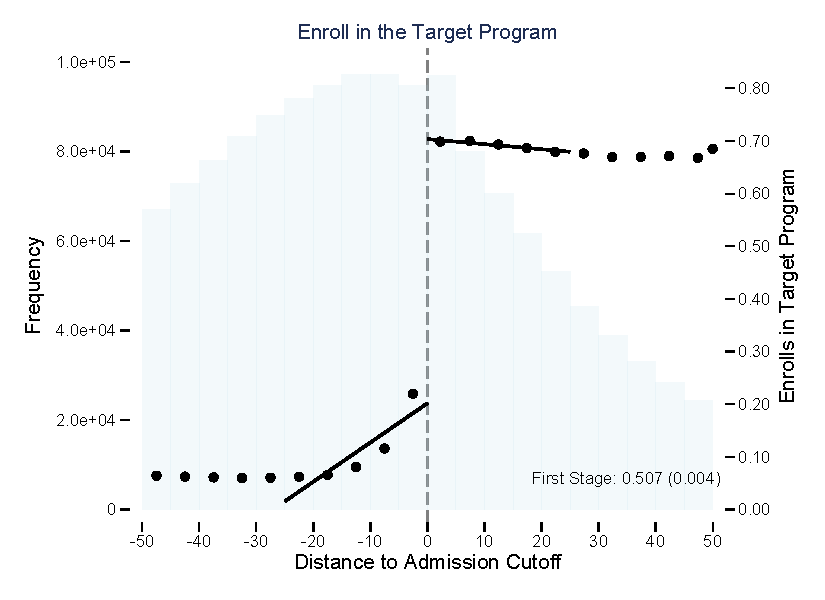
\includegraphics[width=\linewidth]{../../output/figures/Enrolls/rd_enrolls_target.pdf}

\column{0.25\textwidth}

\small

\textbf{RDD estimate}
{\small 0.507}
{\small (0.004)}

\vspace{0.3cm}

Crossing the cutoff increases target-program enrollment by approximately 51 percentage points.



\end{columns}

\end{frame}


\begin{frame}{Enrollment on University and HE Program}
\begin{columns}

\column{0.48\textwidth}

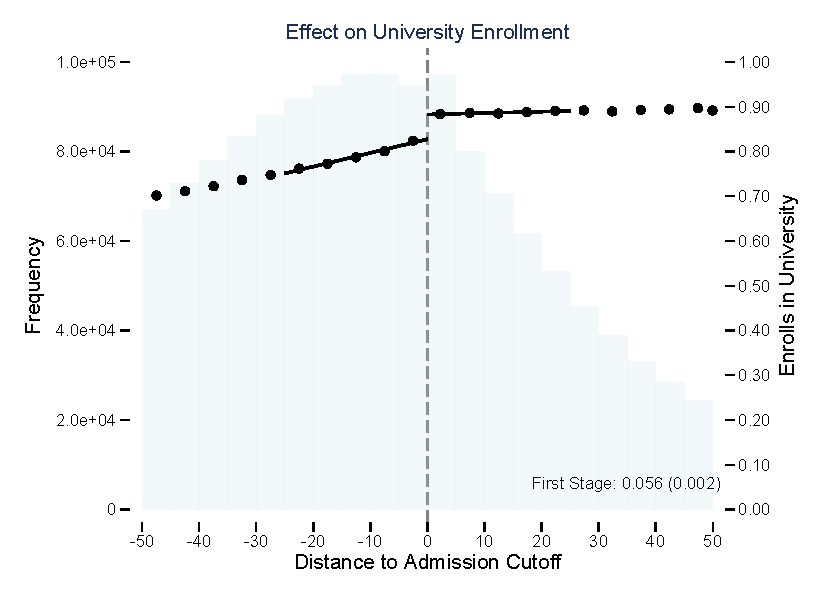
\includegraphics[width=\linewidth]{../../output/figures/Enrolls/rd_enrolls_uni.pdf}


\column{0.48\textwidth}

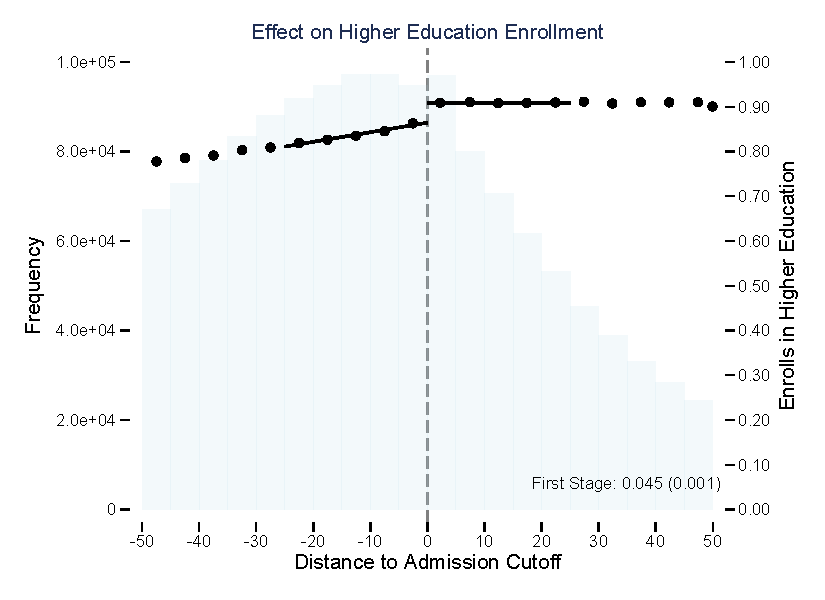
\includegraphics[width=\linewidth]{../../output/figures/Enrolls/rd_enrolls_he.pdf}

\end{columns}

\vspace{0.25cm}

\small

\begin{itemize}
\item Most applicants below the cutoff still access university or higher education through alternative options.
\item Crossing the cutoff mainly changes \textbf{where students enroll}, rather than \textbf{whether they enroll}.
\end{itemize}

\end{frame}
%---------------------------------------------------
%----------------------------------------------------
\begin{frame}{Target Enrollment Within Three Years}

\begin{columns}

\column{0.75\textwidth}

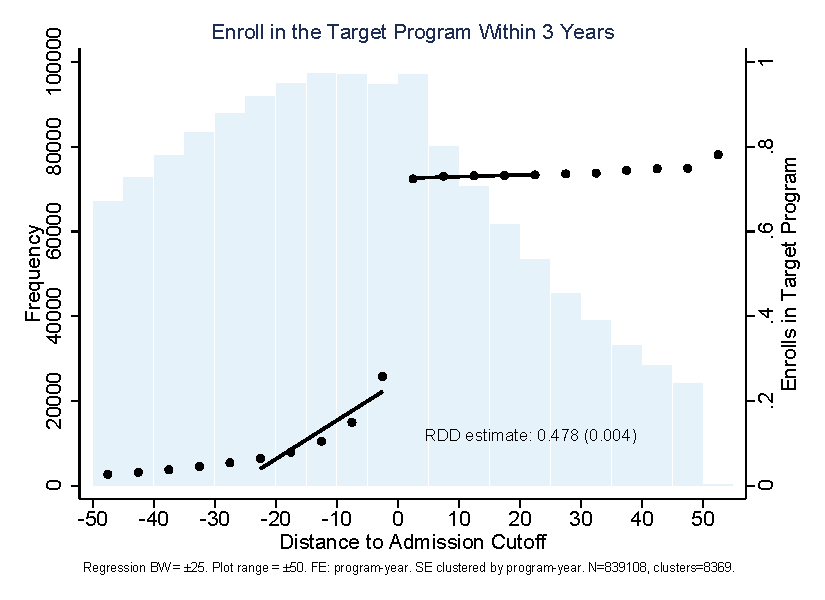
\includegraphics[width=\linewidth]{../../output/figures/enrollment_3y/rdd_enrolls_target_3y.pdf}

\column{0.25\textwidth}

\small

\textbf{RDD estimate}

{\small 0.478}

{\small (0.004)}

\vspace{0.3cm}

Crossing the cutoff increases target-program enrollment within three years by approximately 48 percentage points.

\end{columns}

\end{frame}
%---------------------------------------------------
%----------------------------------------------------
\begin{frame}{Broader Enrollment Outcomes Within Three Years}

\begin{columns}

\column{0.48\textwidth}

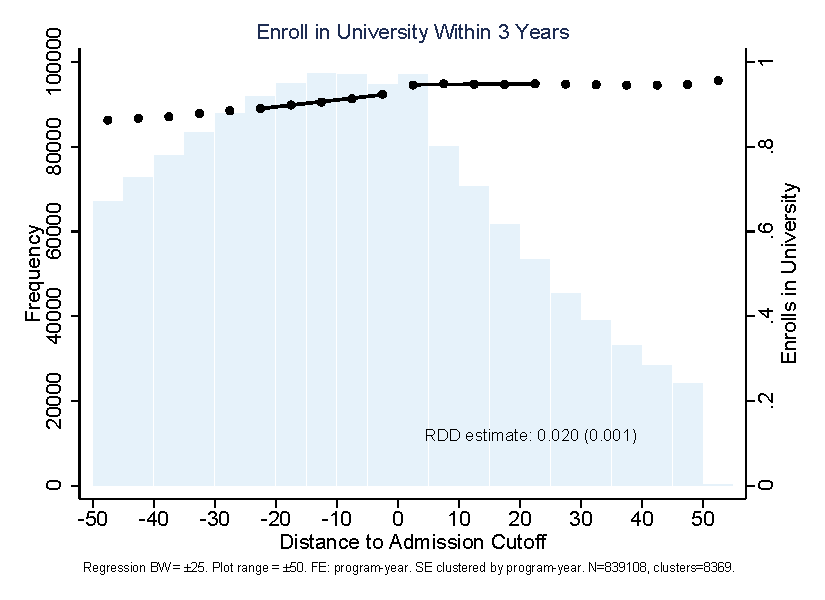
\includegraphics[width=\linewidth]{../../output/figures/enrollment_3y/rdd_enrolls_uni_3y.pdf}

\column{0.48\textwidth}

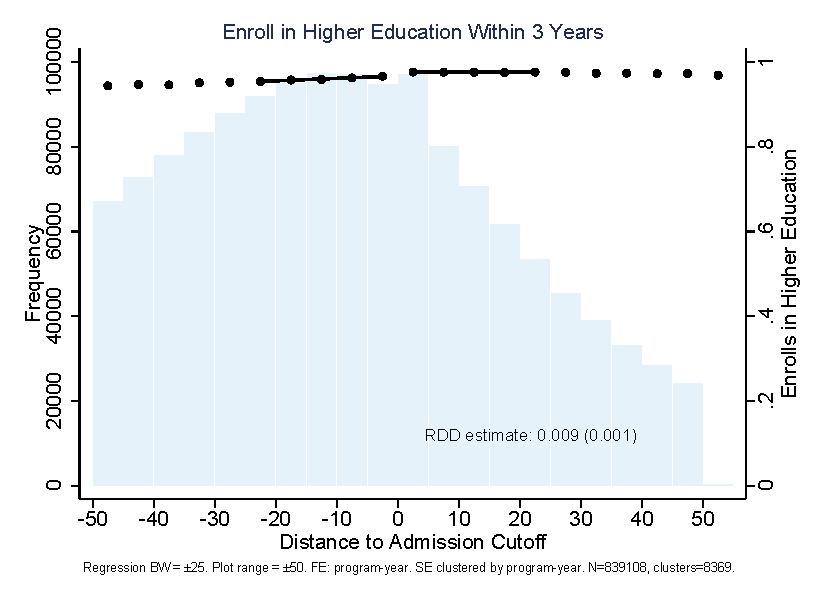
\includegraphics[width=\linewidth]{../../output/figures/enrollment_3y/rdd_enrolls_he_3y.pdf}

\end{columns}

\vspace{0.25cm}

\small

\begin{itemize}
\item Most applicants below the cutoff still access university or higher education through alternative options.

\item The effect on overall higher-education participation remains small.

\item The main effect continues to operate through the specific program attended.
\end{itemize}

\end{frame}
%---------------------------------------------------

\begin{frame}{PSU Retaking Within Two Years}

\centering

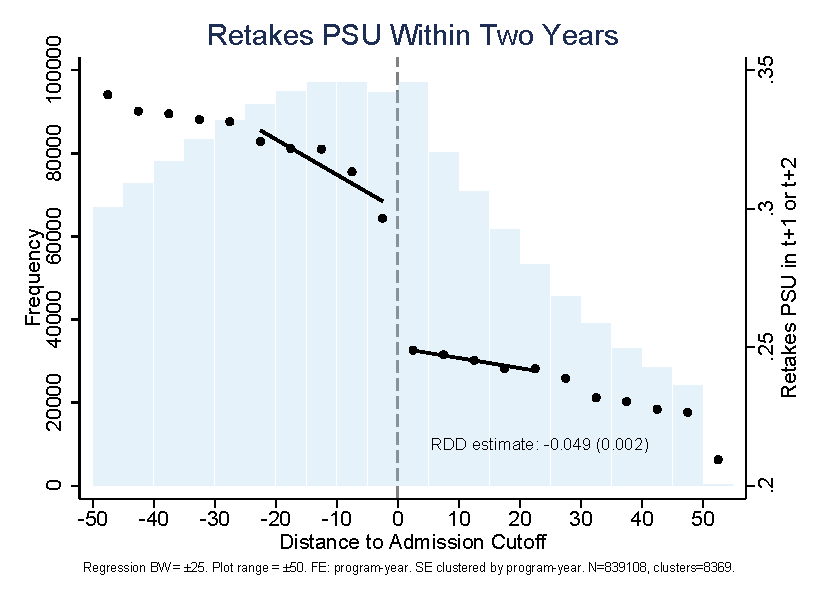
\includegraphics[width=0.7\textwidth]{../../output/figures/retakes_psu/rdd_retakes_psu_2y.pdf}

\small

\begin{itemize}
\item Crossing the cutoff reduces PSU retaking within the next two years.

\item Applicants above the cutoff are less likely to re-enter the admission process.

\item Admission eligibility lowers incentives to improve future admission outcomes.
\end{itemize}

\end{frame}

%====================================================
%----------------------------------------------------
\begin{frame}{Target Graduation Within Eight Years}

\begin{columns}

\column{0.75\textwidth}

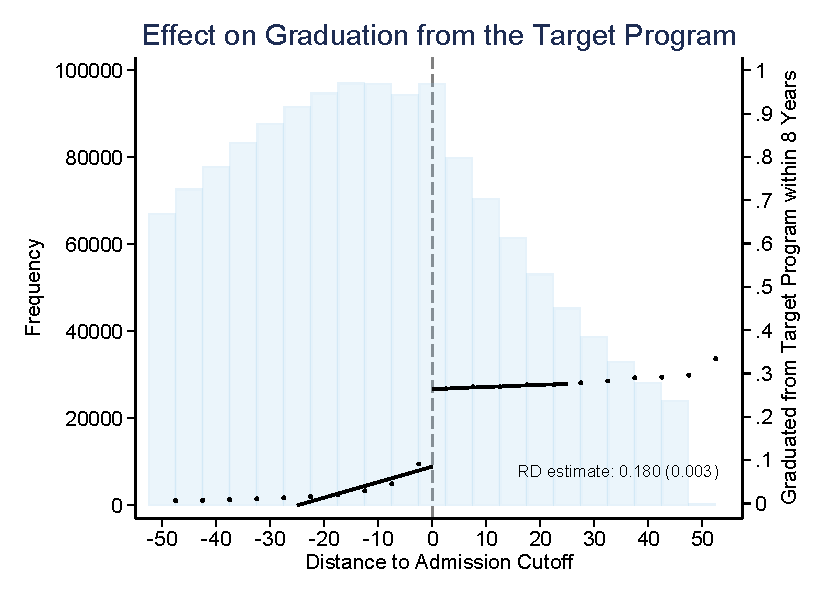
\includegraphics[width=\linewidth]{../../output/figures/Graduates/graduation_8y/rd_graduates_target_8y.pdf}

\column{0.25\textwidth}

\small

\textbf{RDD estimate}

{\small 0.180}

{\small (0.003)}

\vspace{0.3cm}

Crossing the cutoff increases graduation from the target program by approximately 18 percentage points.

\end{columns}

\vspace{0.2cm}

\footnotesize
Graduation is measured within eight years of the application year.

\end{frame}
%----------------------------------------------------
%----------------------------------------------------
\begin{frame}{Broader Graduation Outcomes Within Eight Years}

\begin{columns}

\column{0.48\textwidth}

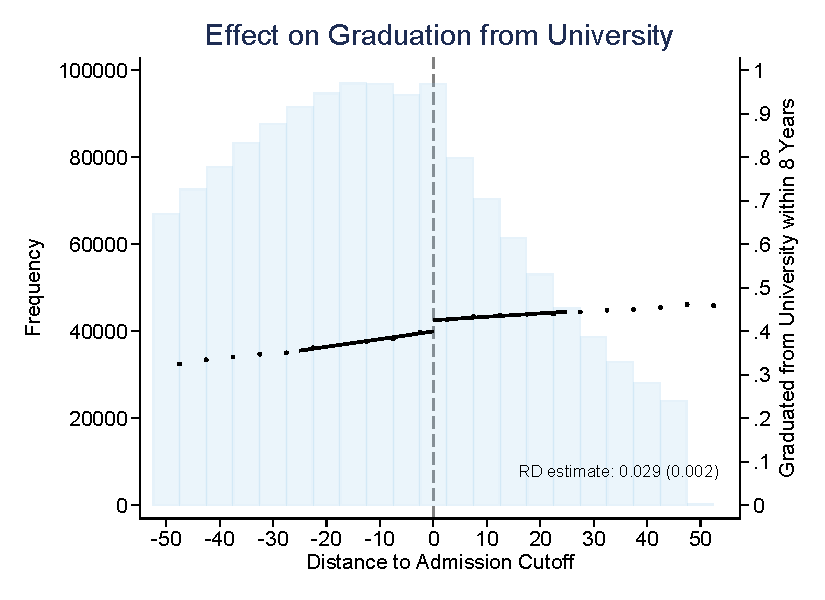
\includegraphics[width=\linewidth]{../../output/figures/Graduates/graduation_8y/rd_graduates_uni_8y.pdf}

\column{0.48\textwidth}

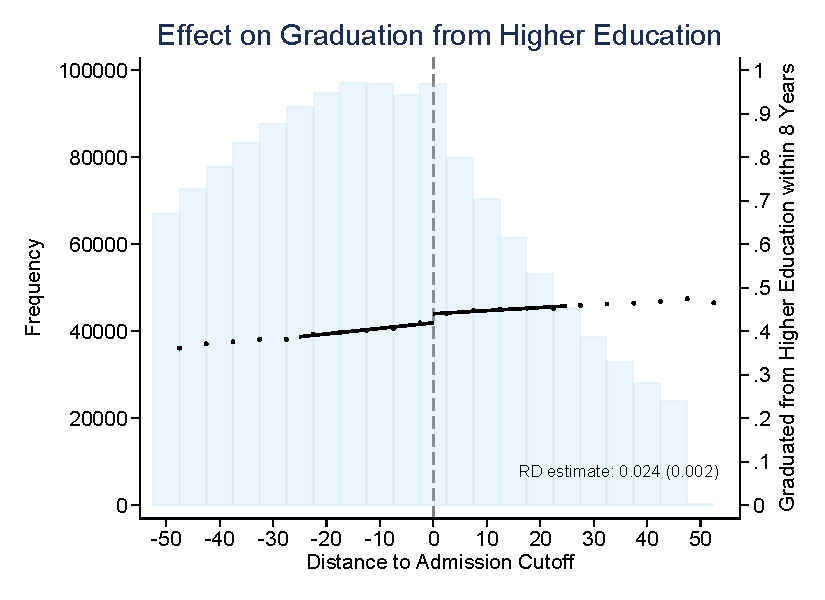
\includegraphics[width=\linewidth]{../../output/figures/Graduates/graduation_8y/rd_graduates_he_8y.pdf}

\end{columns}

\vspace{0.25cm}

\small

\begin{itemize}
\item Broader graduation effects are positive but much smaller than the target-program effect.

\item Crossing the cutoff mainly changes where students graduate, rather than whether they complete higher education.

\end{itemize}

\end{frame}
%----------------------------------------------------

\subsection{Heterogeneity}
%----------------------------------------------------
\begin{frame}{Target Enrollment Effects by Field}

\centering

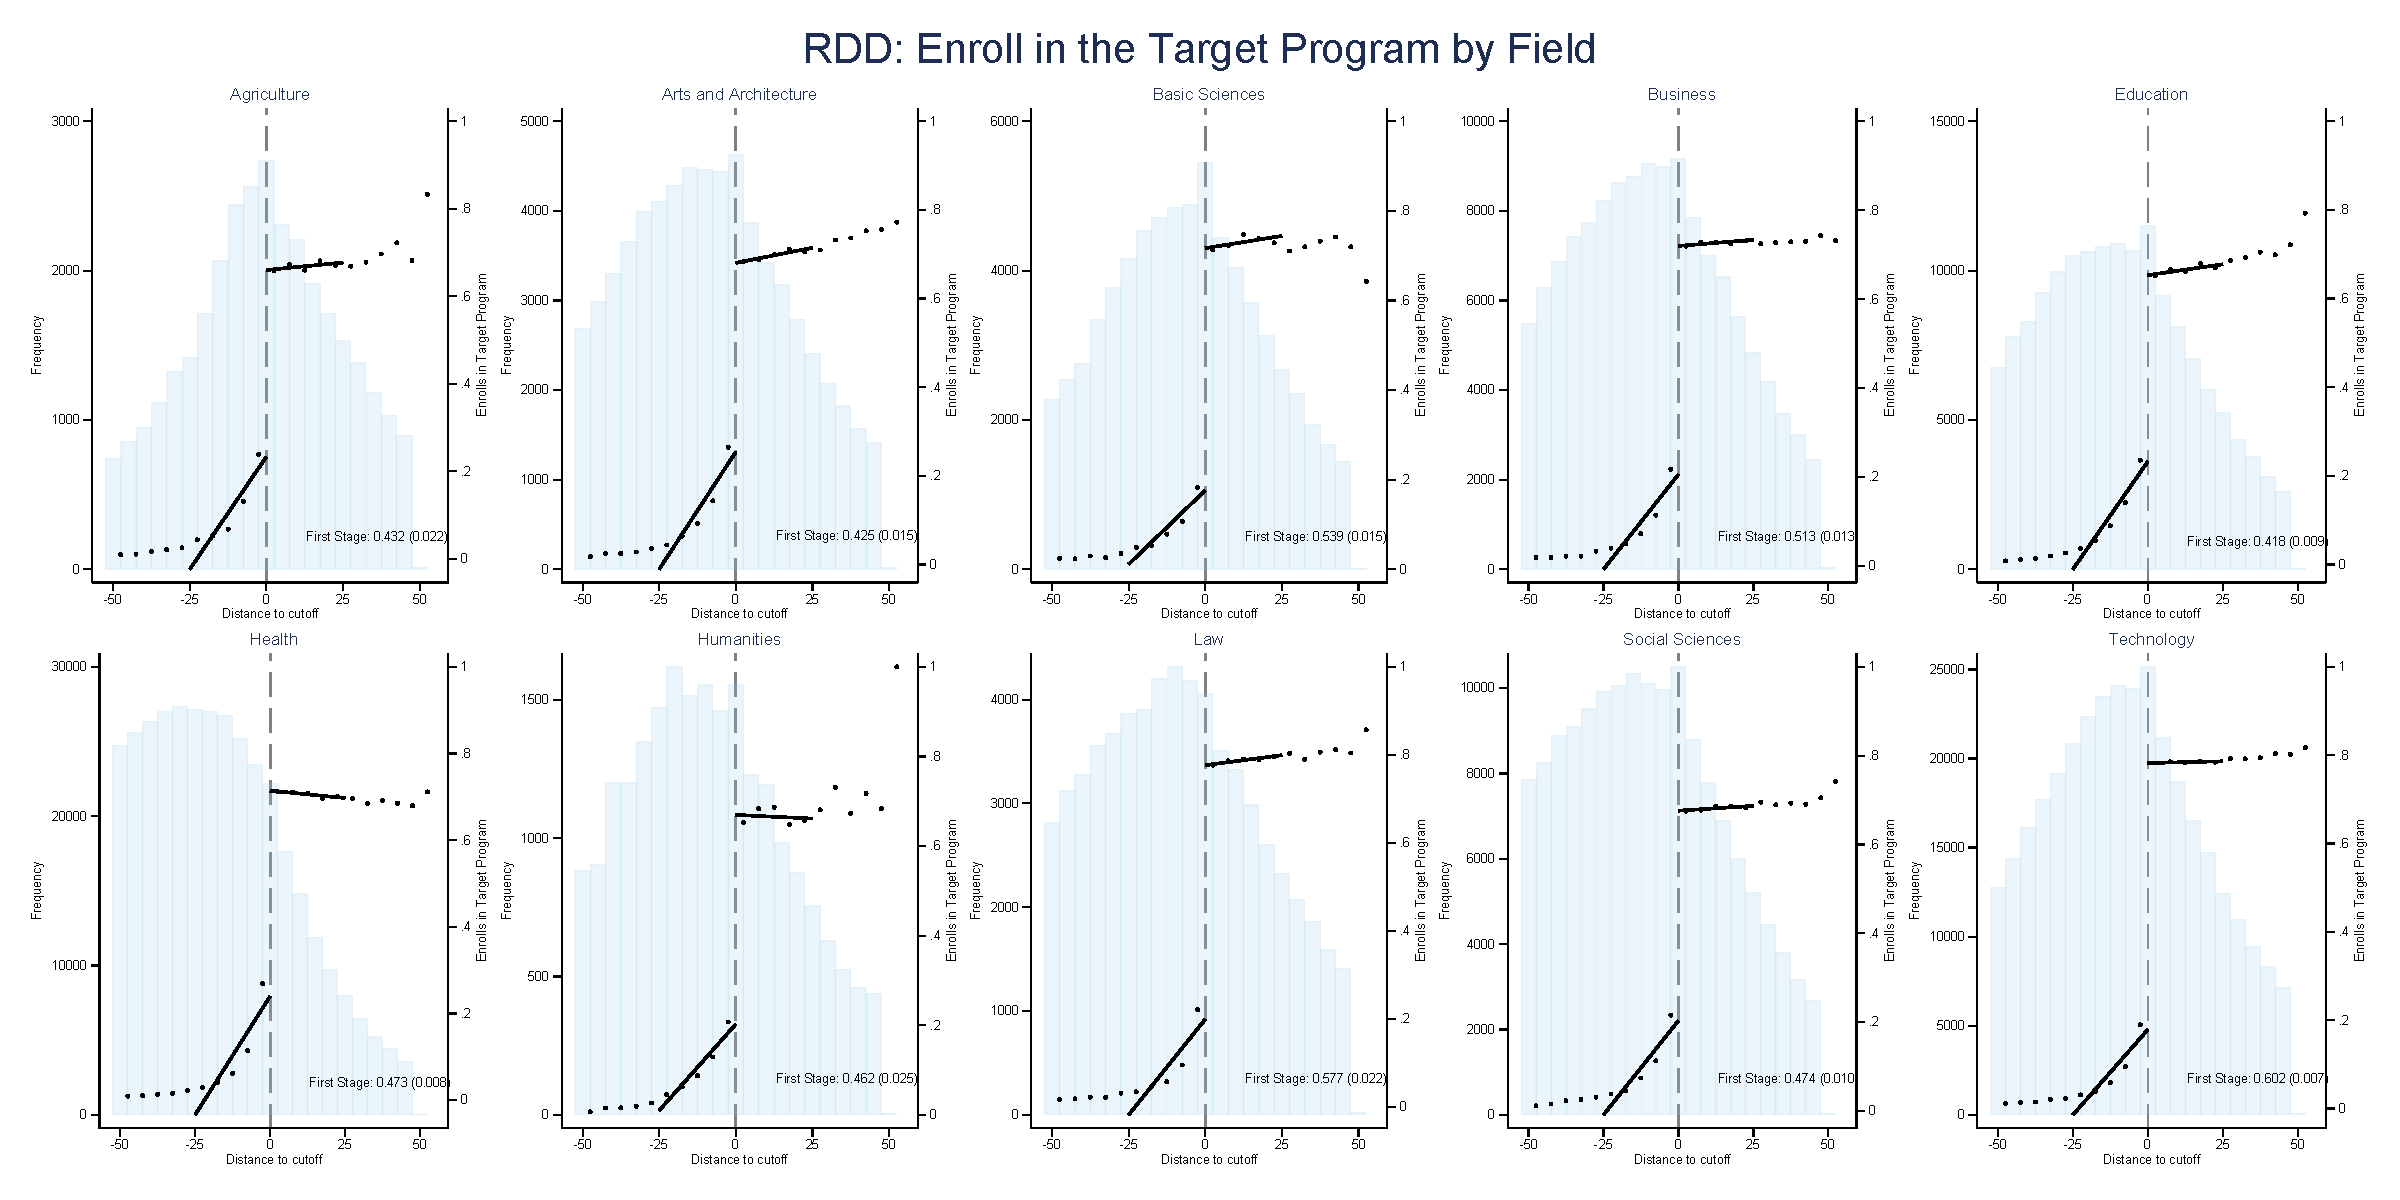
\includegraphics[width=0.90\textwidth]{../../output/figures/Enrolls/by_field/combined/combined_rd_enrolls_target_by_field.pdf}

\vspace{0.15cm}

\small

\begin{itemize}
    \item Crossing the cutoff increases target-program enrollment in every field.
    \item Effects are largest in Technology, Law, Basic Sciences, and Business.
\end{itemize}

\end{frame}
%----------------------------------------------------
%----------------------------------------------------
\begin{frame}{Target Enrollment Effects by Field}

\centering
\scriptsize
\begin{tabular}{lcccc}
\toprule
Field & Target & University & HE & N \\
\midrule
Agriculture & 0.432 & 0.083 & 0.065 & 21,102 \\
Arts \& Architecture & 0.425 & 0.041 & 0.034 & 39,715 \\
Basic Sciences & 0.539 & 0.072 & 0.063 & 43,849 \\
Business & 0.513 & 0.051 & 0.034 & 79,964 \\
Education & 0.418 & 0.057 & 0.044 & 95,508 \\
Health & 0.473 & 0.043 & 0.039 & 206,050 \\
Humanities & 0.462 & 0.092 & 0.084 & 13,470 \\
Law & 0.577 & 0.054 & 0.054 & 37,000 \\
Social Sciences & 0.474 & 0.057 & 0.049 & 90,504 \\
Technology & 0.602 & 0.063 & 0.047 & 211,145 \\
\bottomrule
\end{tabular}
\end{frame}
%----------------------------------------------------

\begin{frame}{University enrollment effects by field.}

\centering
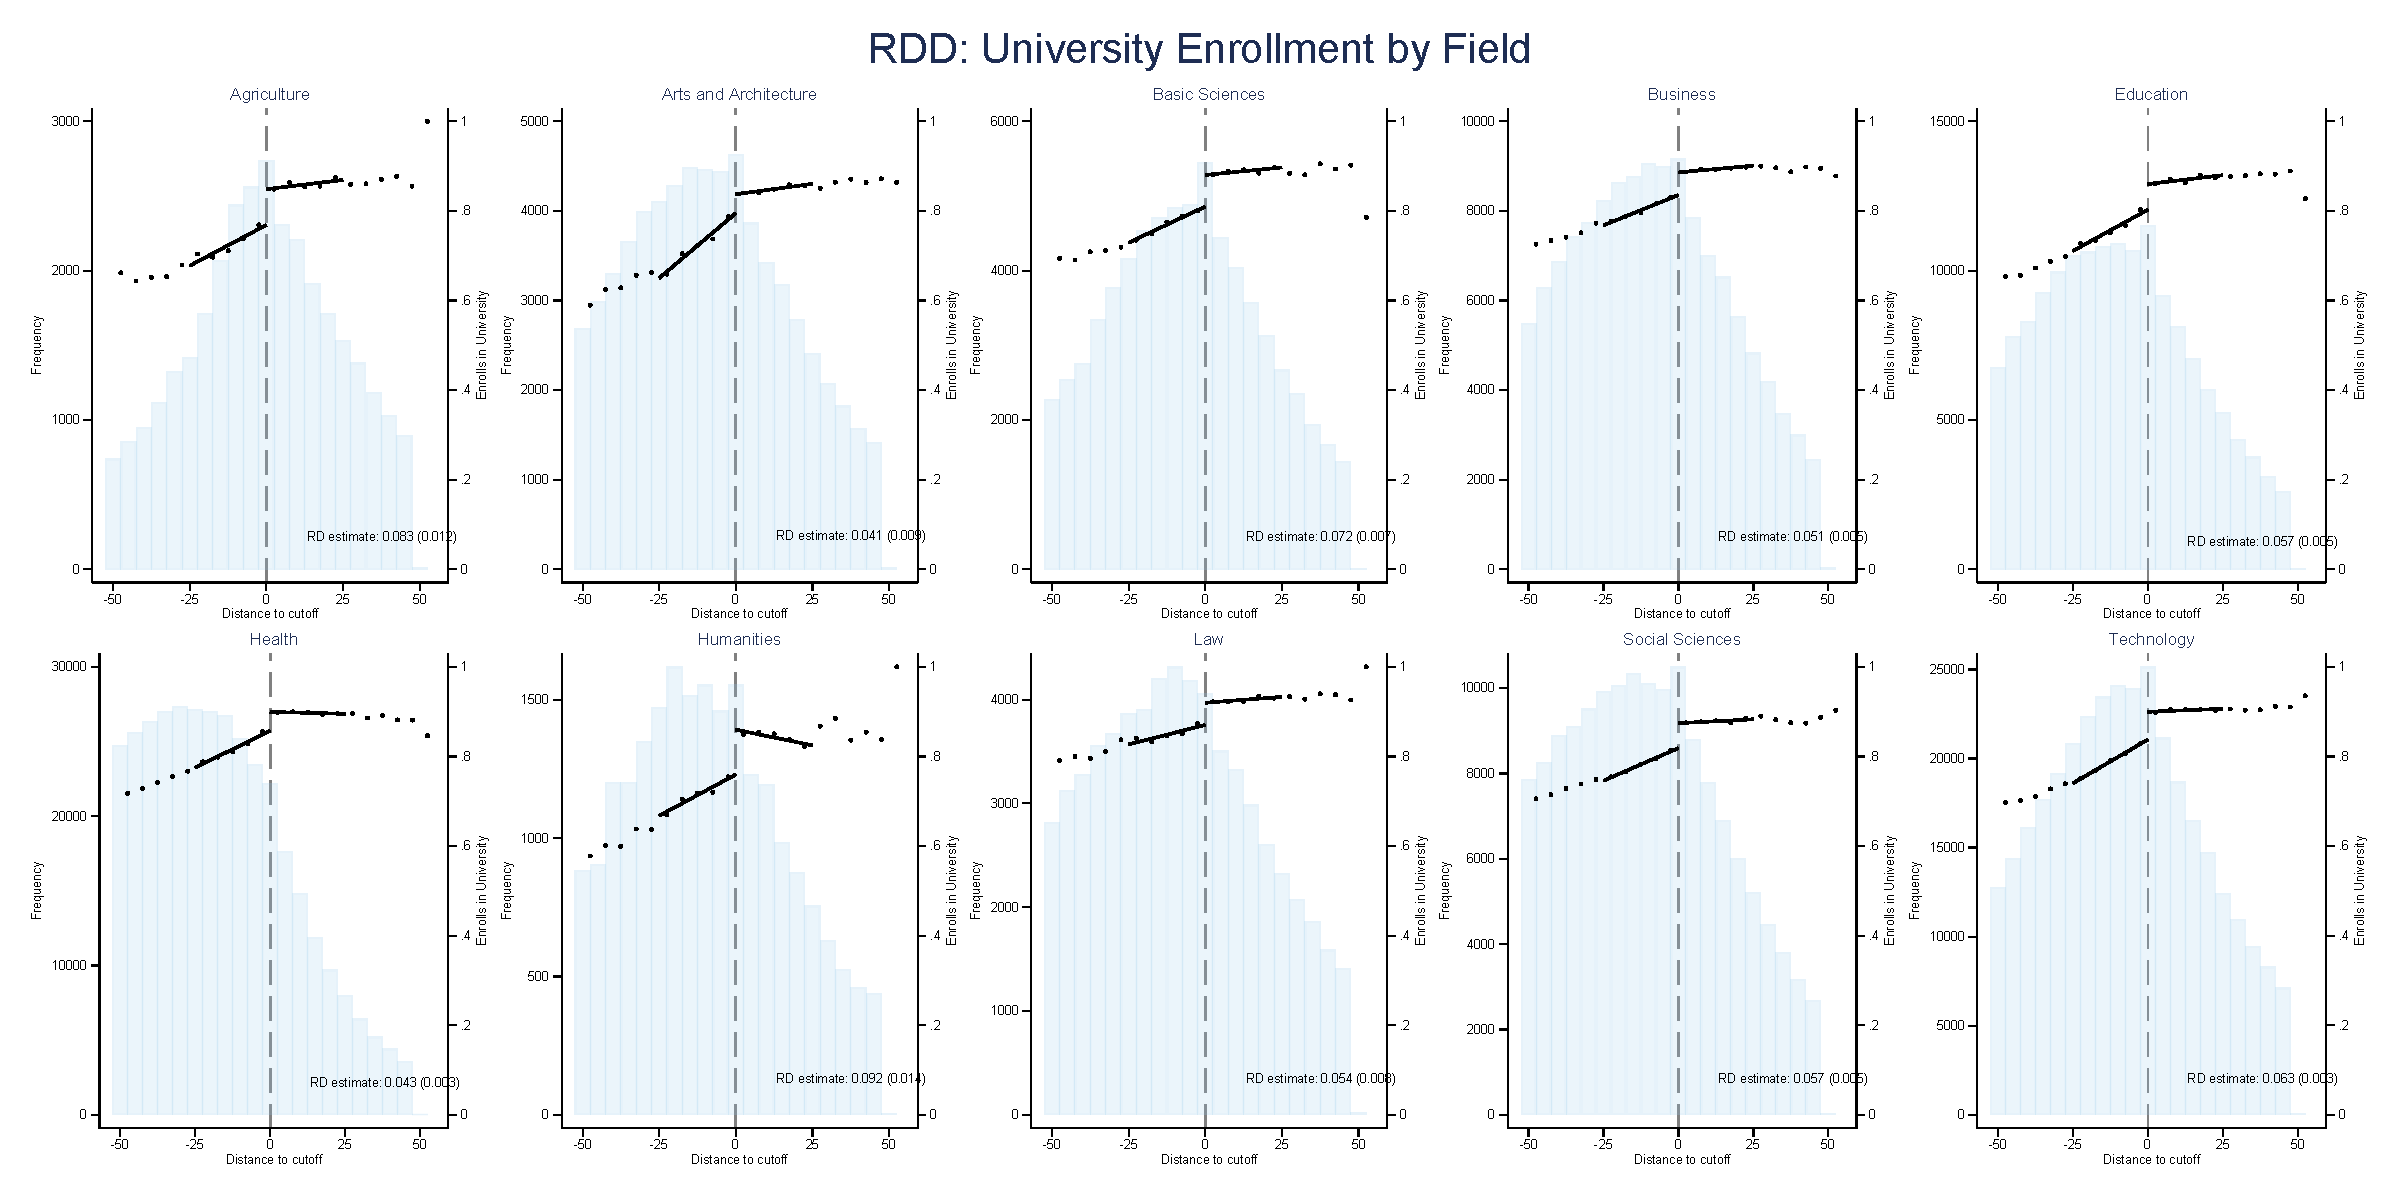
\includegraphics[width=0.95\textwidth]{../../output/figures/Enrolls/by_field/combined/combined_rd_enrolls_uni_by_field.pdf}

\end{frame}

\begin{frame}{Higher-education enrollment effects by field}

\centering
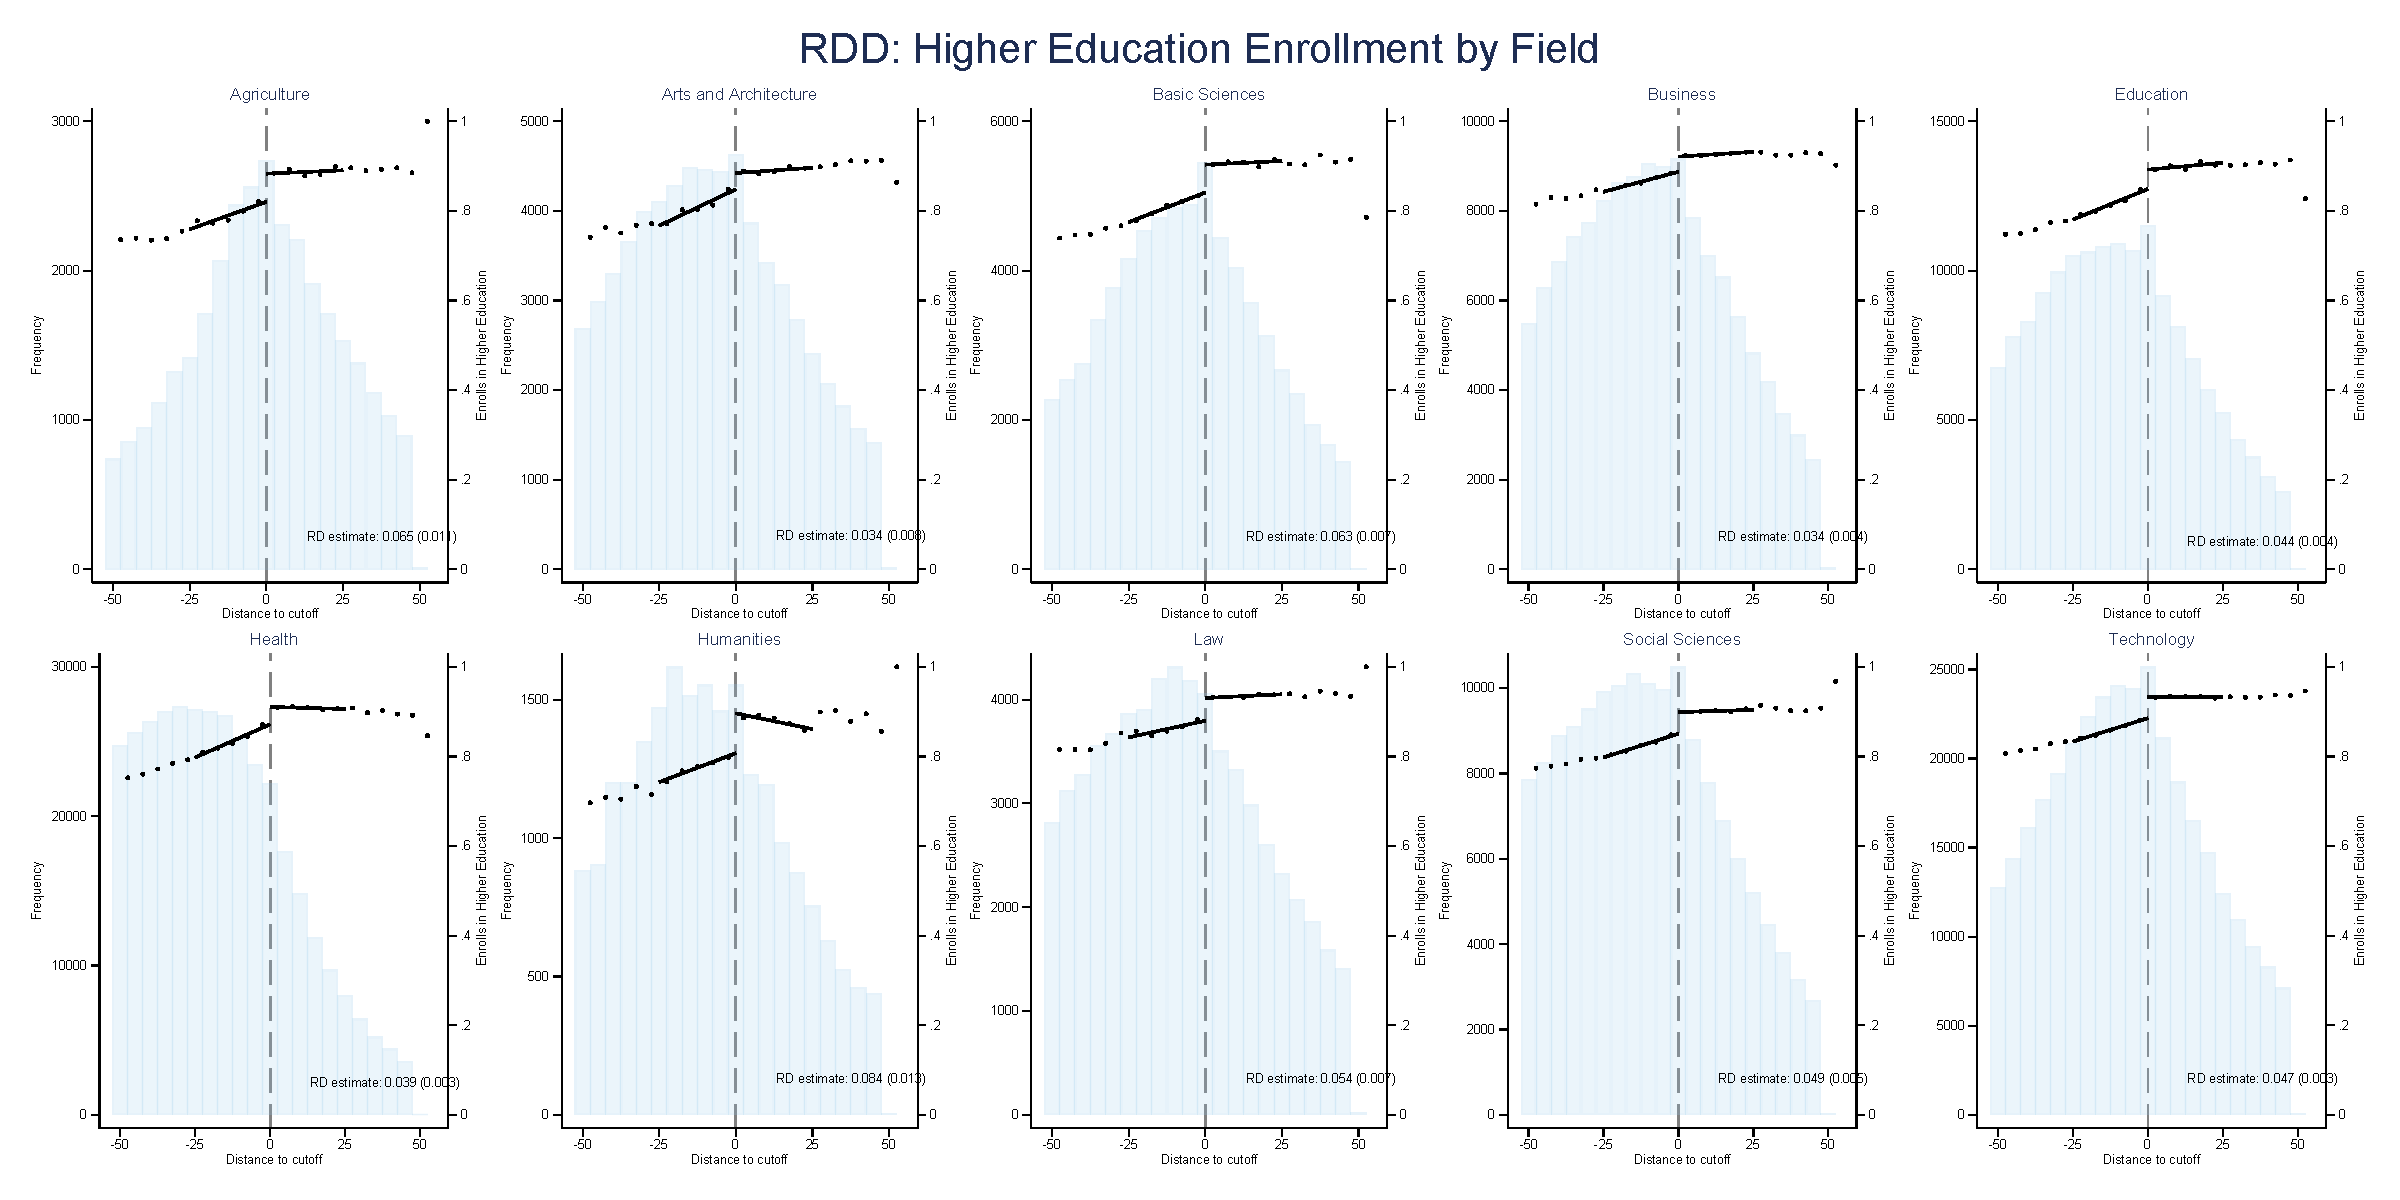
\includegraphics[width=0.95\textwidth]{../../output/figures/Enrolls/by_field/combined/combined_rd_enrolls_he_by_field.pdf}
\end{frame}


%----------------------------------------------------
\begin{frame}{RDD estimates by field: university and HE enrollment}

\centering
\tiny

\begin{tabular}{llcccc}
\toprule
Field & Outcome & Estimate & SE & N & Baseline \\
\midrule
Agriculture & University & 0.083 & 0.012 & 21,102 & 0.729 \\
            & HE         & 0.065 & 0.011 & 21,102 & 0.793 \\
\midrule
Arts \& Architecture & University & 0.041 & 0.009 & 39,715 & 0.723 \\
                     & HE         & 0.034 & 0.008 & 39,715 & 0.808 \\
\midrule
Basic Sciences & University & 0.072 & 0.007 & 43,849 & 0.771 \\
               & HE         & 0.063 & 0.007 & 43,849 & 0.809 \\
\midrule
Business & University & 0.051 & 0.005 & 79,964 & 0.802 \\
         & HE         & 0.034 & 0.004 & 79,964 & 0.865 \\
\midrule
Education & University & 0.057 & 0.005 & 95,508 & 0.757 \\
          & HE         & 0.044 & 0.004 & 95,508 & 0.815 \\
\midrule
Health & University & 0.043 & 0.003 & 206,050 & 0.815 \\
       & HE         & 0.039 & 0.003 & 206,050 & 0.834 \\
\midrule
Humanities & University & 0.092 & 0.014 & 13,470 & 0.713 \\
           & HE         & 0.084 & 0.013 & 13,470 & 0.775 \\
\midrule
Law & University & 0.054 & 0.008 & 37,000 & 0.849 \\
    & HE         & 0.054 & 0.007 & 37,000 & 0.862 \\
\midrule
Social Sciences & University & 0.057 & 0.005 & 90,504 & 0.782 \\
                & HE         & 0.049 & 0.005 & 90,504 & 0.824 \\
\midrule
Technology & University & 0.063 & 0.003 & 211,145 & 0.790 \\
           & HE         & 0.047 & 0.003 & 211,145 & 0.860 \\
\bottomrule
\end{tabular}

\end{frame}
%----------------------------------------------------

%----------------------------------------------------
\begin{frame}{Target Graduation Effects by Field}

\centering

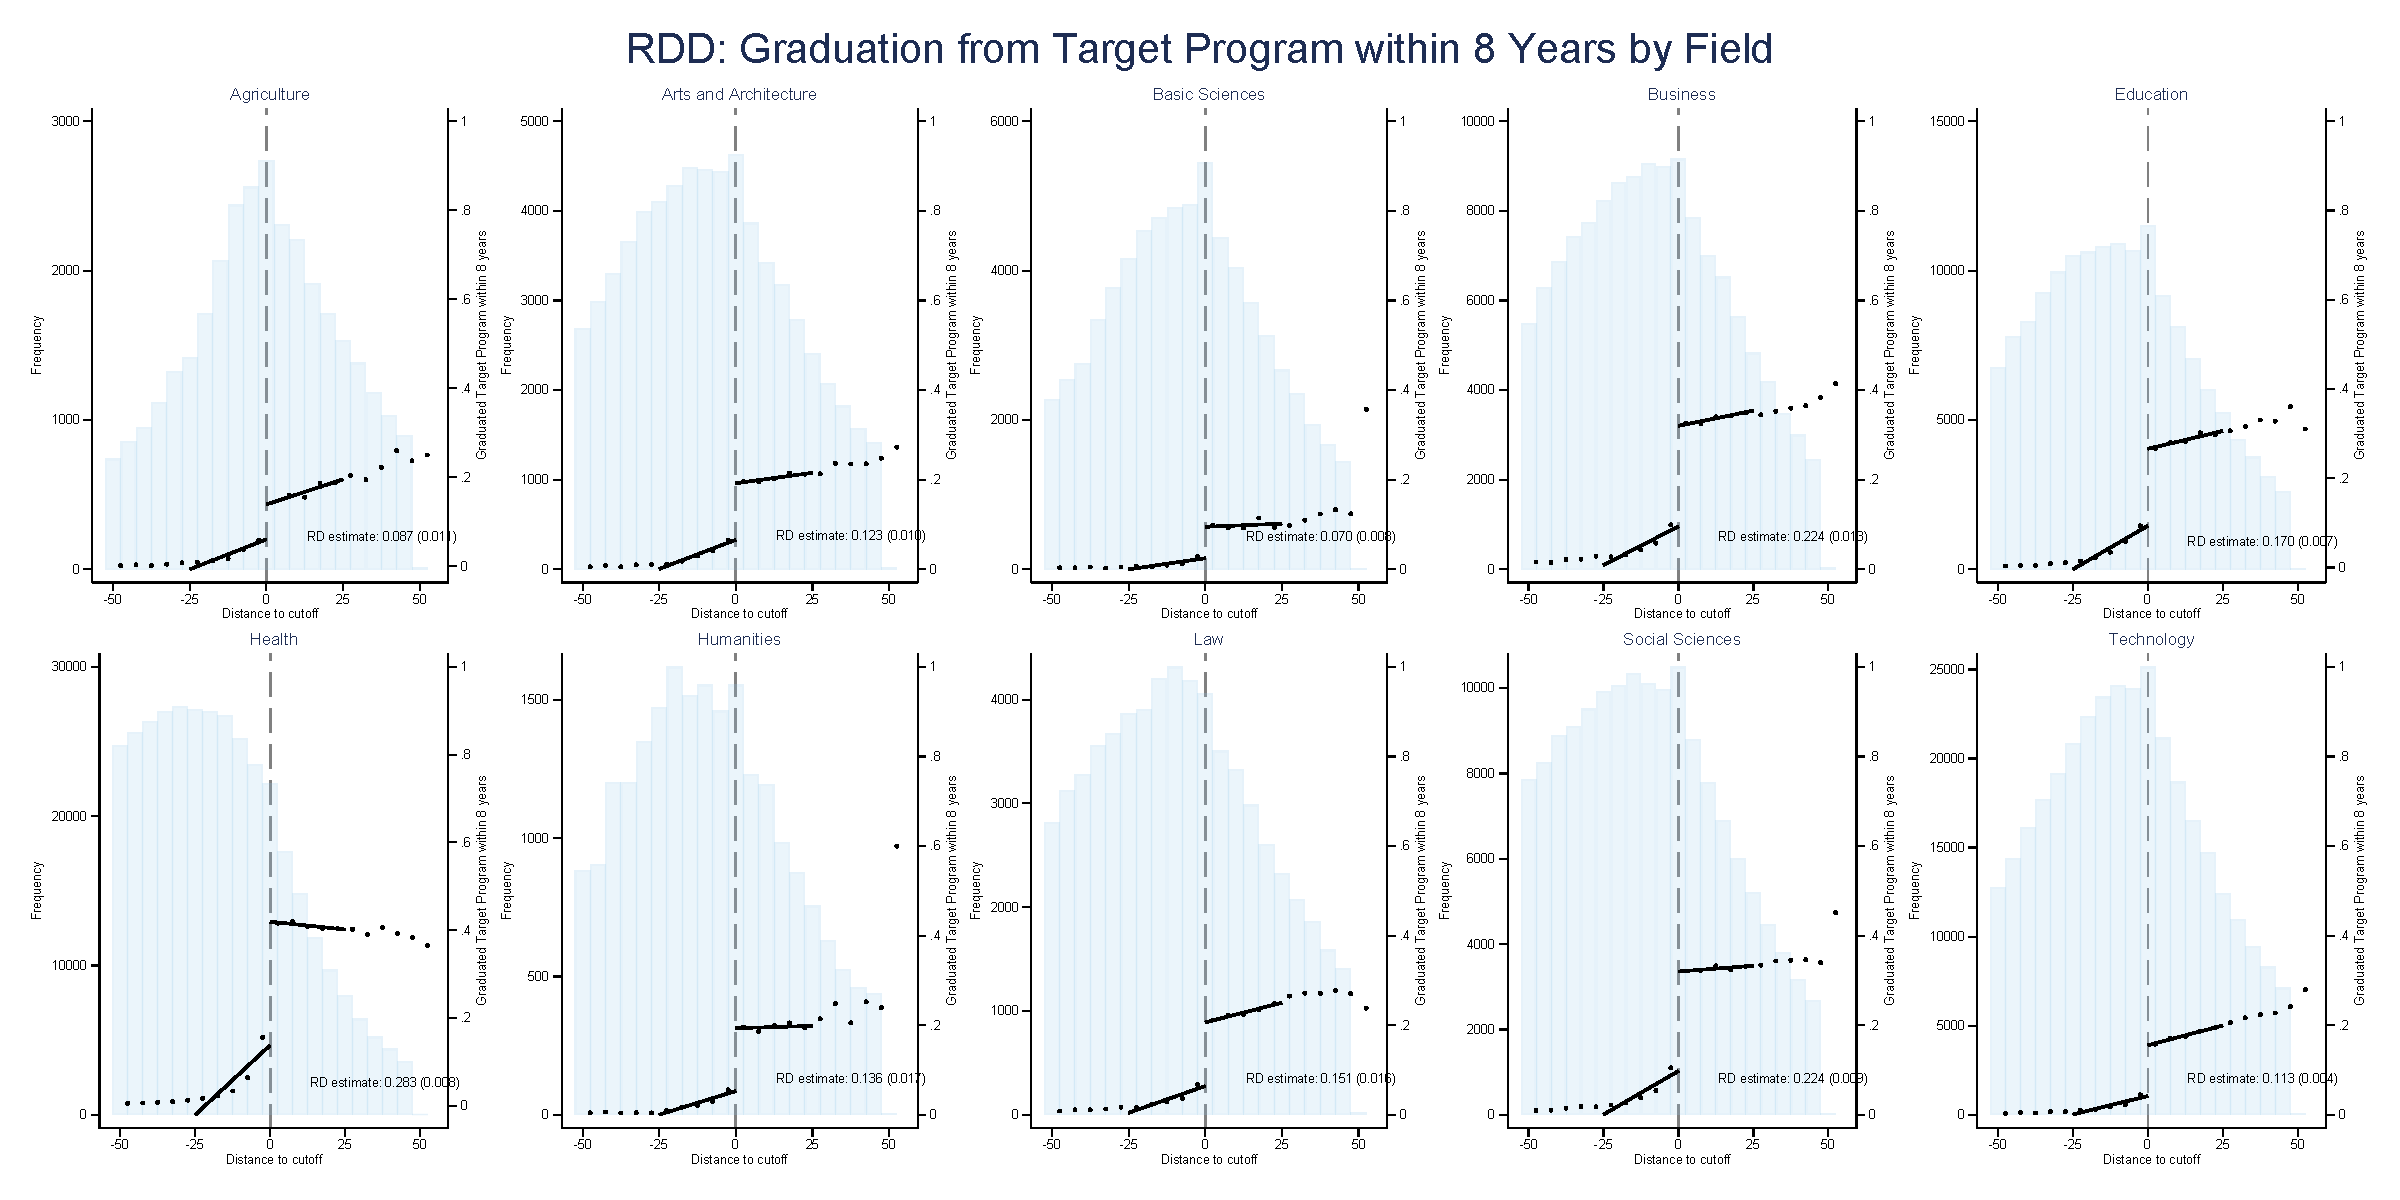
\includegraphics[width=0.90\textwidth]{../../output/figures/Graduates/graduation_8y/combined_by_field/combined_rd_graduates_target_8y_by_field.pdf}

\vspace{0.15cm}

\small

\begin{itemize}
    \item Crossing the cutoff increases target-program graduation across all fields.
    \item The largest effects appear in Health, Business, Social Sciences, Education, and Law.
\end{itemize}
\end{frame}
%----------------------------------------------------
\begin{frame}{RDD estimates by field: target graduation}

\begin{table}
\centering
\scriptsize
\begin{tabular}{lcc}
\toprule
Field & Estimate & SE \\
\midrule
Agriculture & 0.087 & 0.011 \\
Arts \& Architecture & 0.123 & 0.010 \\
Basic Sciences & 0.070 & 0.008 \\
Business & 0.224 & 0.013 \\
Education & 0.170 & 0.007 \\
Health & 0.283 & 0.008 \\
Humanities & 0.136 & 0.017 \\
Law & 0.151 & 0.016 \\
Social Sciences & 0.224 & 0.009 \\
Technology & 0.113 & 0.004 \\
\bottomrule
\end{tabular}
\end{table}


\end{frame}

%====================================================

\begin{frame}{Graduation effects by field: university}

\centering
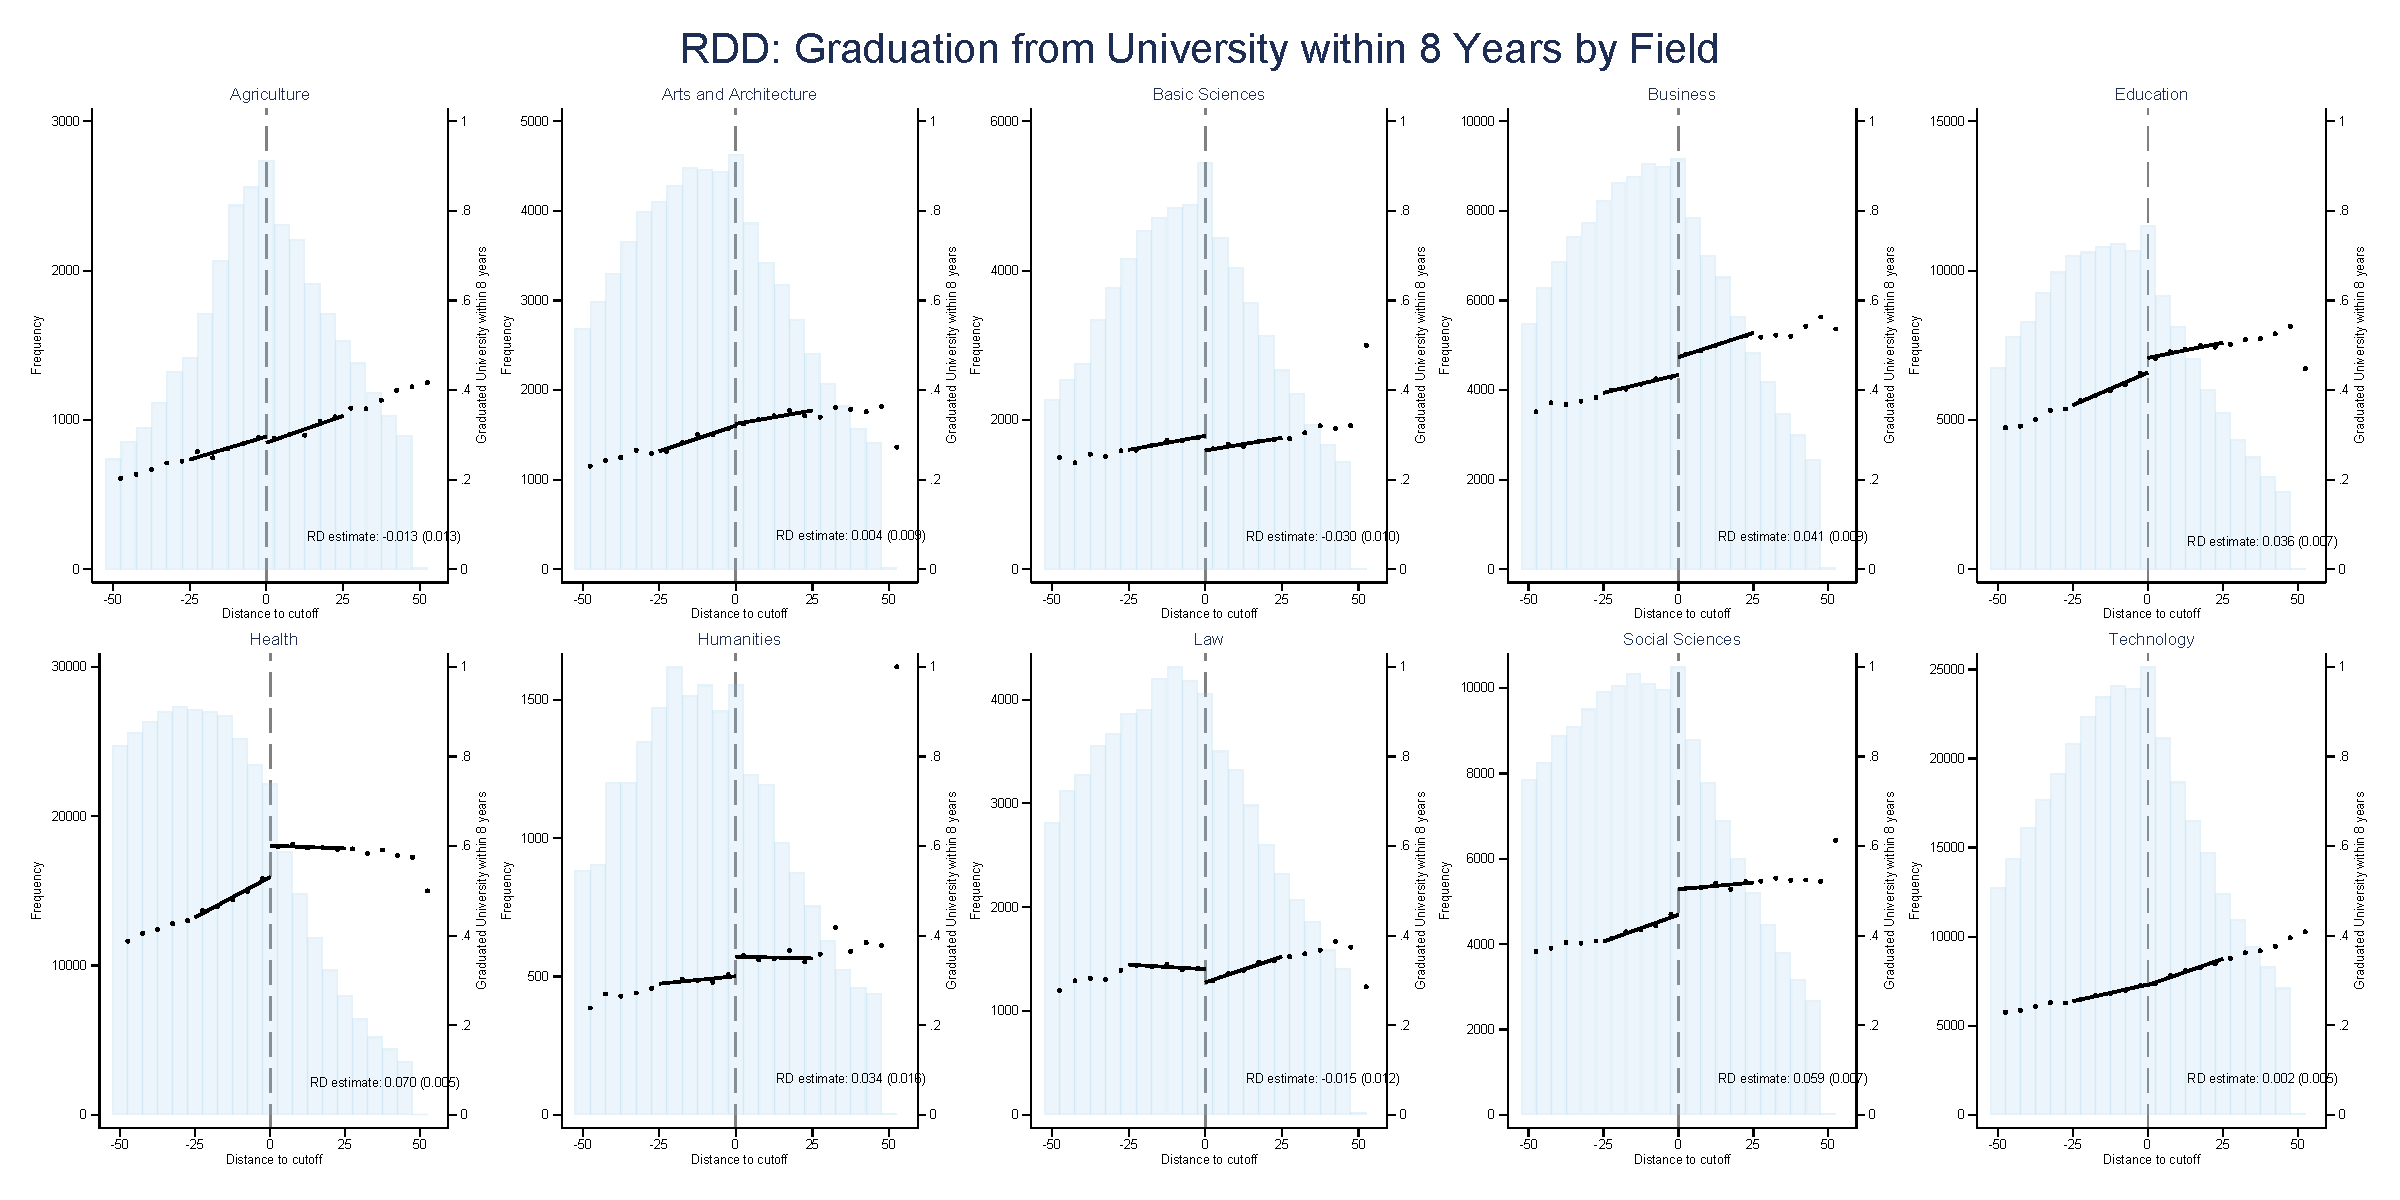
\includegraphics[width=0.95\textwidth]{../../output/figures/Graduates/graduation_8y/combined_by_field/combined_rd_graduates_uni_8y_by_field.pdf}

\end{frame}


\begin{frame}{Graduation effects by field: any higher education}

\centering
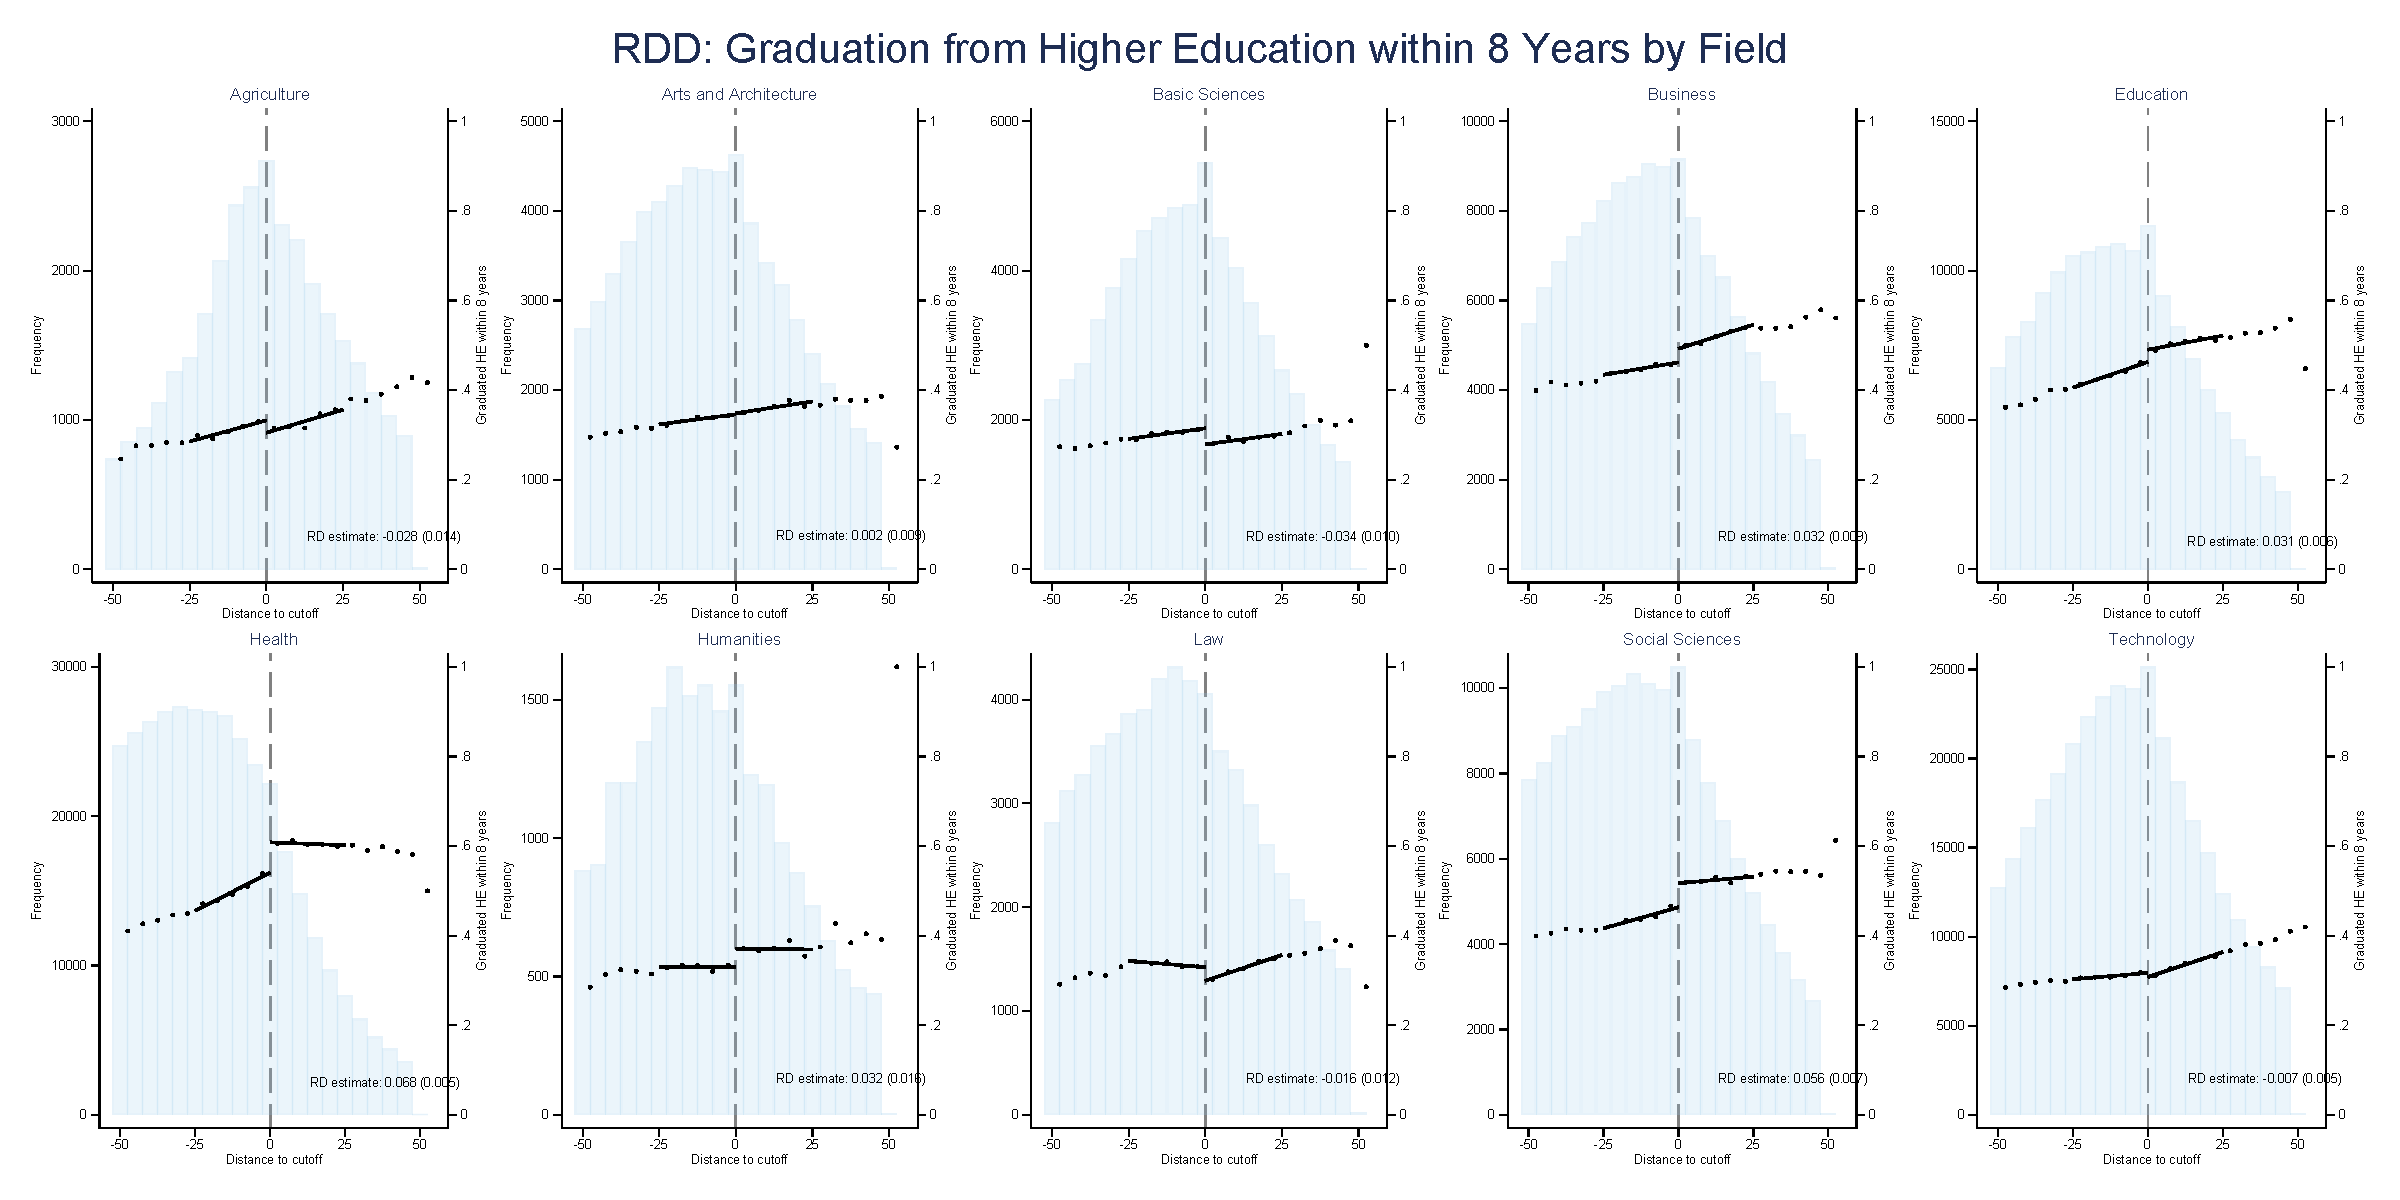
\includegraphics[width=0.95\textwidth]{../../output/figures/Graduates/graduation_8y/combined_by_field/combined_rd_graduates_he_8y_by_field.pdf}

\end{frame}

\begin{frame}{RDD estimates by field: university and HE graduation}

\centering
\tiny

\begin{tabular}{llcccc}
\toprule
Field & Outcome & Estimate & SE & N & Baseline \\
\midrule
Agriculture & University & -0.013 & 0.013 & 21,102 & 0.274 \\
            & HE         & -0.028 & 0.014 & 21,102 & 0.312 \\
\midrule
Arts \& Architecture & University & 0.004 & 0.009 & 39,715 & 0.292 \\
                     & HE         & 0.002 & 0.009 & 39,715 & 0.335 \\
\midrule
Basic Sciences & University & -0.030 & 0.010 & 43,849 & 0.283 \\
               & HE         & -0.034 & 0.010 & 43,849 & 0.303 \\
\midrule
Business & University & 0.041 & 0.009 & 79,964 & 0.414 \\
         & HE         & 0.032 & 0.009 & 79,964 & 0.448 \\
\midrule
Education & University & 0.036 & 0.007 & 95,508 & 0.403 \\
          & HE         & 0.031 & 0.006 & 95,508 & 0.434 \\
\midrule
Health & University & 0.070 & 0.005 & 206,050 & 0.484 \\
       & HE         & 0.068 & 0.005 & 206,050 & 0.497 \\
\midrule
Humanities & University & 0.034 & 0.016 & 13,470 & 0.301 \\
           & HE         & 0.032 & 0.016 & 13,470 & 0.330 \\
\midrule
Law & University & -0.015 & 0.012 & 37,000 & 0.330 \\
    & HE         & -0.016 & 0.012 & 37,000 & 0.337 \\
\midrule
Social Sciences & University & 0.059 & 0.007 & 90,504 & 0.417 \\
                & HE         & 0.056 & 0.007 & 90,504 & 0.440 \\
\midrule
Technology & University & 0.002 & 0.005 & 211,145 & 0.273 \\
           & HE         & -0.007 & 0.005 & 211,145 & 0.310 \\
\bottomrule
\end{tabular}

\end{frame}



\subsection{Selective Program-Years}
%----------------------------------------------------
\begin{frame}{Selective Programs: Target Enrollment}

\begin{columns}

\column{0.65\textwidth}

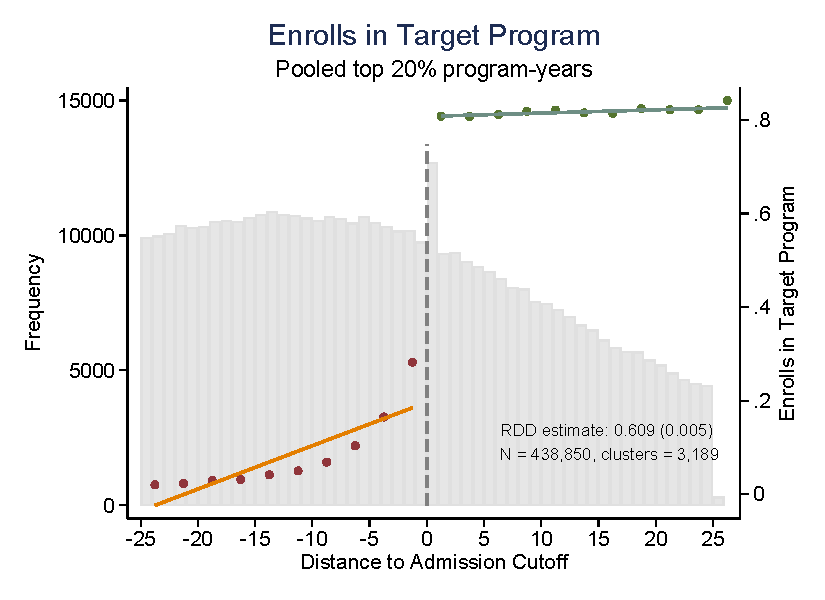
\includegraphics[width=\linewidth]{../../output/figures/Selective/rd_hist_enrolls_target_selective_pooled_top20.pdf}

\column{0.35\textwidth}

\small

\textbf{Selective programs}

\vspace{0.1cm}

\begin{itemize}
    \item Selectivity is based on the Language--Math score distribution of admitted students.

    \item Programs are classified as selective if they appear at least once in the top 20\% of the pooled post-2012 selectivity ranking.
\end{itemize}

\end{columns}

\vspace{0.15cm}

\small
Crossing the cutoff in selective programs increases target-program enrollment by approximately 61 percentage points.

\end{frame}
%----------------------------------------------------
%----------------------------------------------------
\begin{frame}{Selective Programs: Broader Enrollment Outcomes}

\begin{columns}

\column{0.48\textwidth}

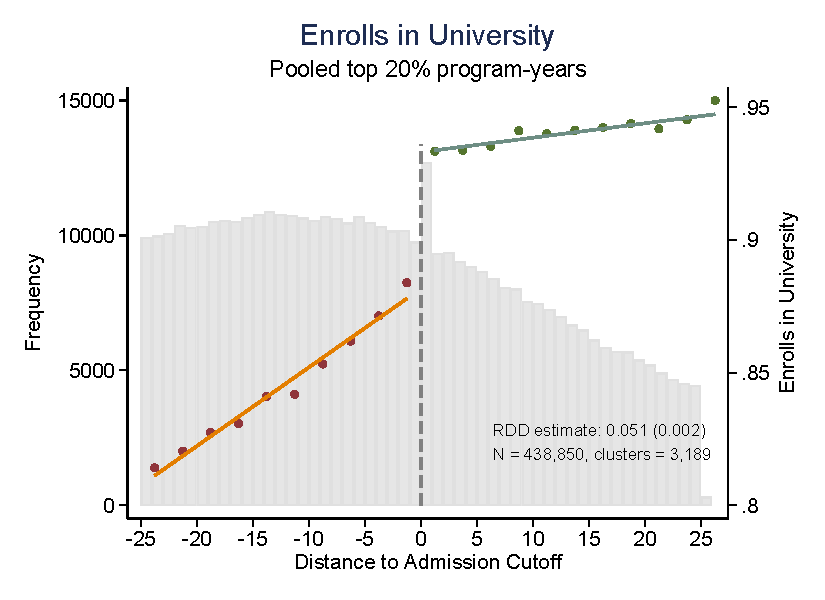
\includegraphics[width=\linewidth]{../../output/figures/Selective/rd_hist_enrolls_uni_selective_pooled_top20.pdf}

\column{0.48\textwidth}

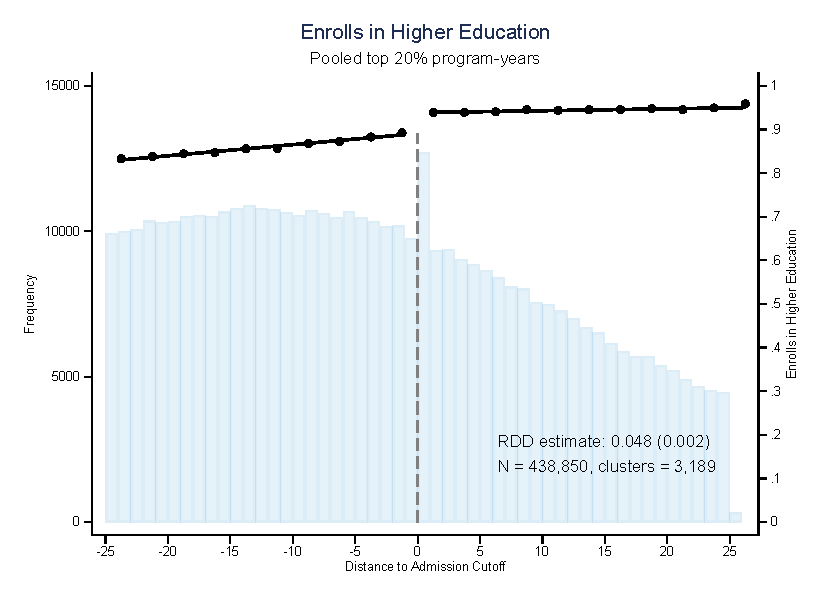
\includegraphics[width=\linewidth]{../../output/figures/Selective/rd_hist_enrolls_he_selective_pooled_top20.pdf}

\end{columns}

\vspace{0.25cm}

\small

\begin{itemize}
    \item Effects on university and higher-education enrollment remain much smaller than target-program enrollment.

    \item Even among selective programs, cutoff crossing mainly changes \textbf{where students enroll}, not overall higher-education participation.
\end{itemize}

\end{frame}
%----------------------------------------------------





%====================================================
\subsection{Selectivity Gaps and Next-Best Alternatives}
%====================================================
\begin{frame}{Construction of Delta Selectivity}

\small

\begin{itemize}
    \item For each target application, we identify the student's next-best feasible alternative.

    \item Program selectivity is measured by the average Language--Math score among regularly admitted students.

    \item We define:
    \[
    \Delta Selectivity =
    Selectivity_{target} - Selectivity_{nextbest}.
    \]

    \item Positive values indicate that the target program is more selective than the next-best alternative.
\end{itemize}

\vspace{-0.1cm}

\begin{table}
\centering
\scriptsize
\begin{tabular}{ll}
\toprule
Group & Definition \\
\midrule
d1 & $\Delta < -10$ \\
d2 & $[-10,10)$ \\
d3 & $[10,30)$ \\
d4 & $[30,50)$ \\
d5 & $\geq 50$ \\
\bottomrule
\end{tabular}
\end{table}

\end{frame}

\begin{frame}{Target Enrollment by Selectivity Gap}

\centering

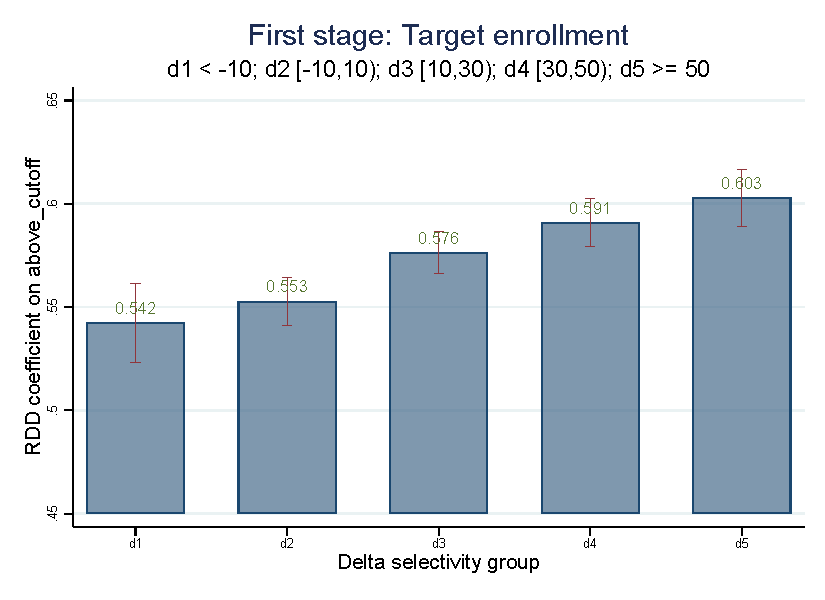
\includegraphics[width=0.6\textwidth]{../../output/figures/delta_groups/fs_target.pdf}


\small

\begin{itemize}
\item Crossing the cutoff increases target-program enrollment across all groups.

\item Effects are strongest when the target program is substantially more selective than the next-best alternative.

\item Admission matters most when students face large differences in program selectivity.
\end{itemize}

\end{frame}


\begin{frame}{Broader Enrollment Outcomes by Selectivity Gap}

\begin{columns}

\column{0.48\textwidth}

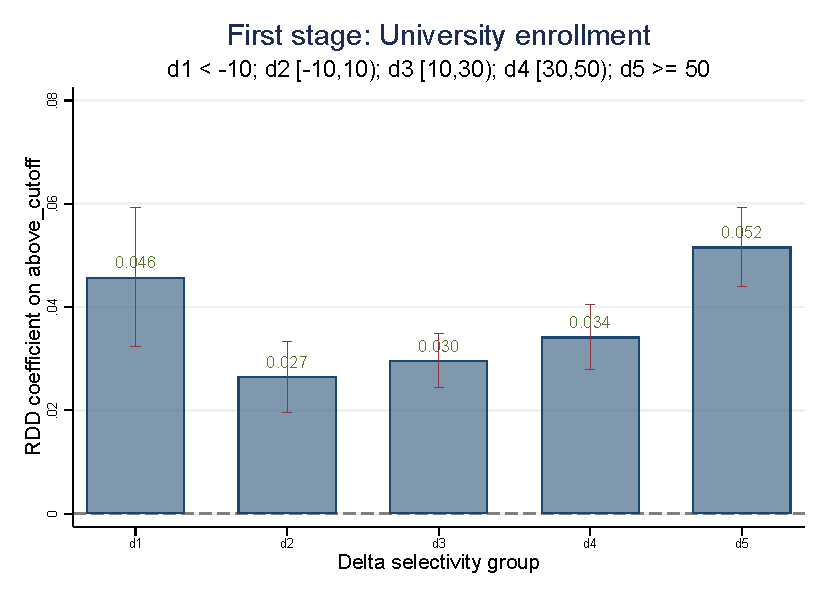
\includegraphics[width=\linewidth]{../../output/figures/delta_groups/fs_uni.pdf}

\column{0.48\textwidth}

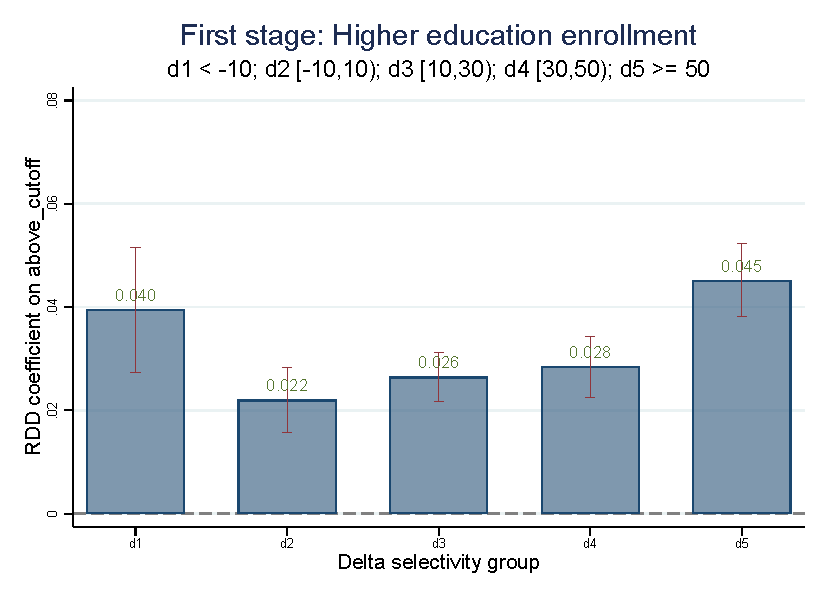
\includegraphics[width=\linewidth]{../../output/figures/delta_groups/fs_he.pdf}

\end{columns}

\vspace{0.25cm}

\small

\begin{itemize}
\item Effects on university and higher-education enrollment remain relatively small across groups.

\item Differences across selectivity-gap groups are much less pronounced than for target-program enrollment.

\item The main response margin remains the specific program attended rather than overall higher-education participation.
\end{itemize}

\end{frame}

%----------------------------------------------------
\begin{frame}{Target Graduation by Selectivity Gap}

\centering

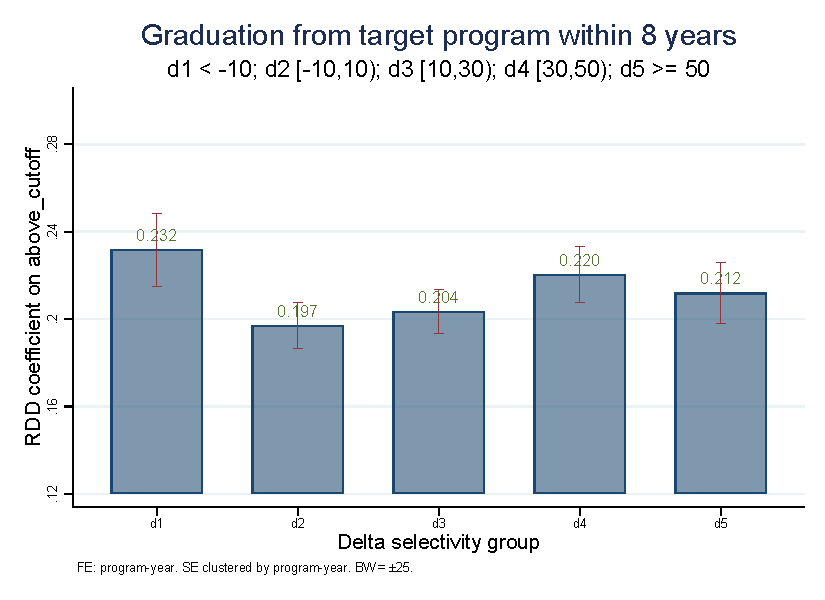
\includegraphics[width=0.6\textwidth]{../../output/figures/delta_groups/rdd_grad_target8y.pdf}

\vspace{0.2cm}

\small

\begin{itemize}
\item Crossing the cutoff increases target-program graduation across all selectivity-gap groups.

\item Target-graduation effects remain large across the distribution of target versus next-best selectivity.


\end{itemize}

\end{frame}
%----------------------------------------------------
%----------------------------------------------------
\begin{frame}{Broader Graduation Outcomes by Selectivity Gap}

\begin{columns}

\column{0.48\textwidth}

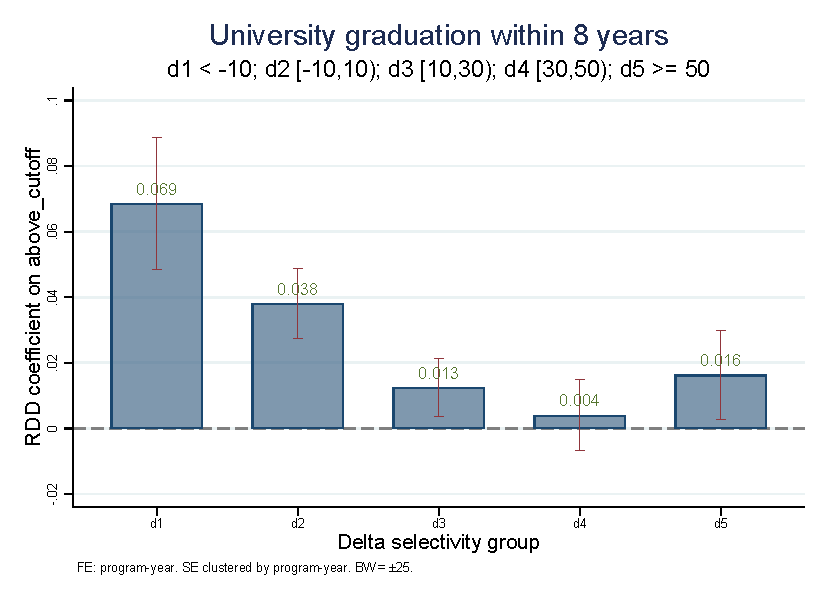
\includegraphics[width=\linewidth]{../../output/figures/delta_groups/rdd_grad_uni8y.pdf}

\column{0.48\textwidth}

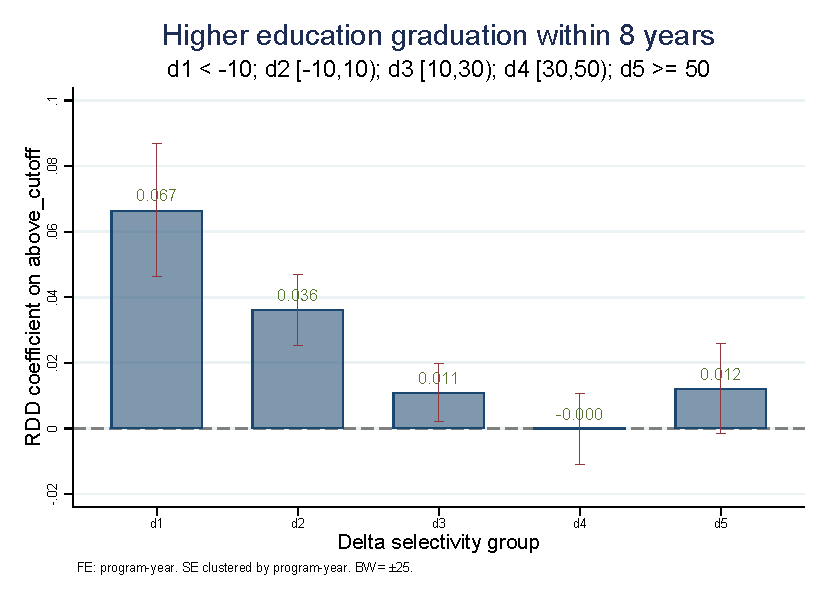
\includegraphics[width=\linewidth]{../../output/figures/delta_groups/rdd_grad_he8y.pdf}

\end{columns}

\vspace{0.25cm}

\small

\begin{itemize}
\item Effects on university and higher-education graduation are smaller than target-program graduation effects.

\item Broader graduation effects are more heterogeneous across selectivity-gap groups.

\item Crossing the cutoff mainly changes where students graduate, rather than whether they complete higher education.
\end{itemize}

\end{frame}
%----------------------------------------------------

\subsection{Same-field vs Different-field Alternatives}

%-------------------------------------------------



\begin{frame}{RDD around cutoff: same field}

\centering
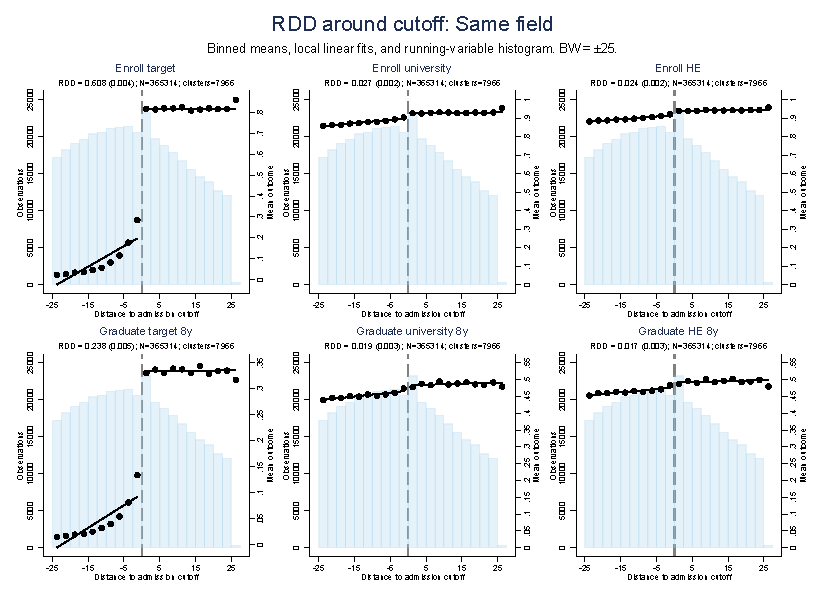
\includegraphics[width=0.7\textwidth]{../../output/figures/same_field_nextbest/rdd_cutoff_same_field_8y.pdf}

\vskip 0.1cm

\tiny
\begin{itemize}
\item Crossing the cutoff generates large increases in target-program enrollment and graduation when the next-best alternative belongs to the same field.

\item Effects on broader university and higher-education outcomes remain small, suggesting that admission mainly affects program choice within a field.
\end{itemize}
\end{frame}

%----------------------------------------------------
\begin{frame}{RDD around cutoff: different field}

\centering
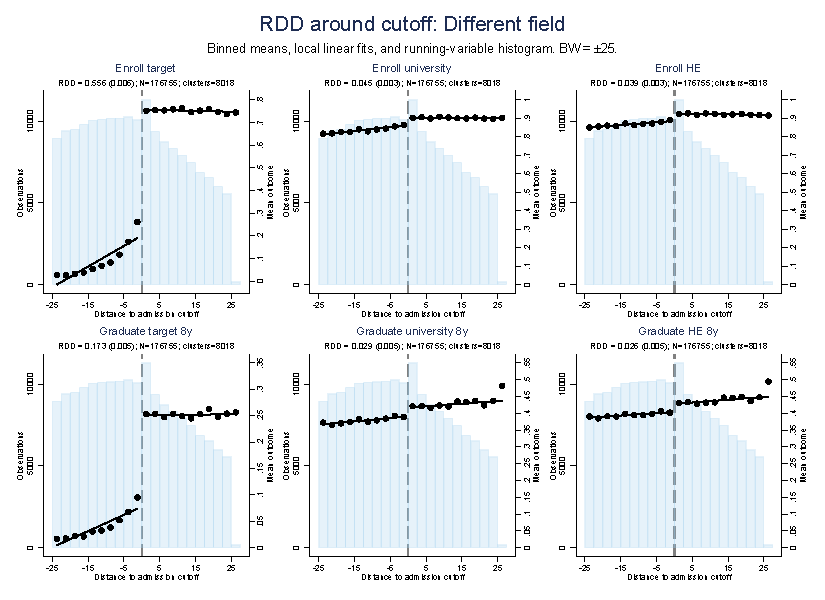
\includegraphics[width=0.7\textwidth]{../../output/figures/same_field_nextbest/rdd_cutoff_different_field_8y.pdf}

\vskip 0.1cm

\tiny
\begin{itemize}
\item Target-program enrollment and graduation effects remain large when the next-best alternative belongs to a different field.
\item Effects on broader university and higher-education outcomes are somewhat larger than in the same-field sample, consistent with admission affecting both program and field choice.
\end{itemize}
\end{frame}

%----------------------------------------------------
\begin{frame}{RDD by selectivity gap: same field}

\centering
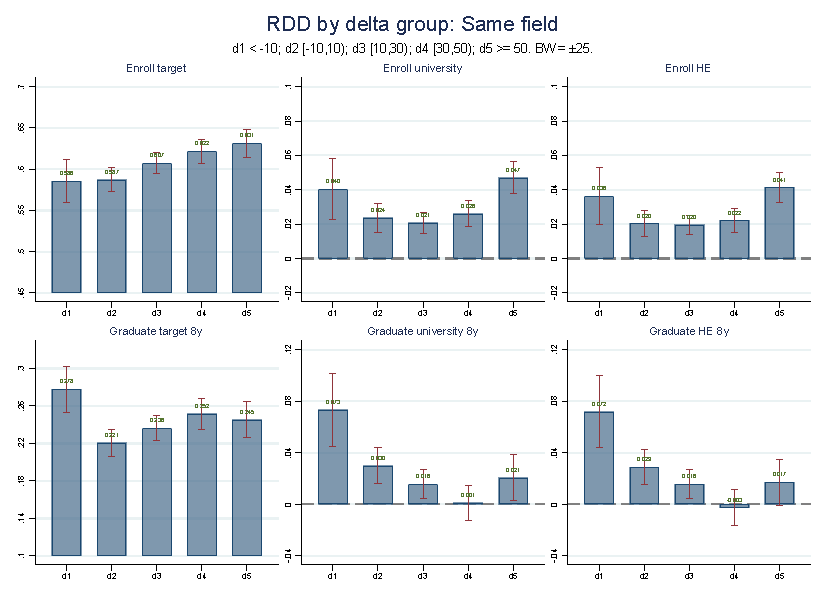
\includegraphics[width=0.7\textwidth]{../../output/figures/same_field_nextbest/rdd_delta_same_field_8y.pdf}

\vskip 0.1cm

\tiny
\begin{itemize}
\item Within same-field alternatives, target-enrollment effects increase with the selectivity gap between the target and next-best program.

\item Broader university and higher-education graduation effects remain comparatively small across groups.
\end{itemize}

\end{frame}

%----------------------------------------------------
\begin{frame}{RDD by selectivity gap: different field}

\centering
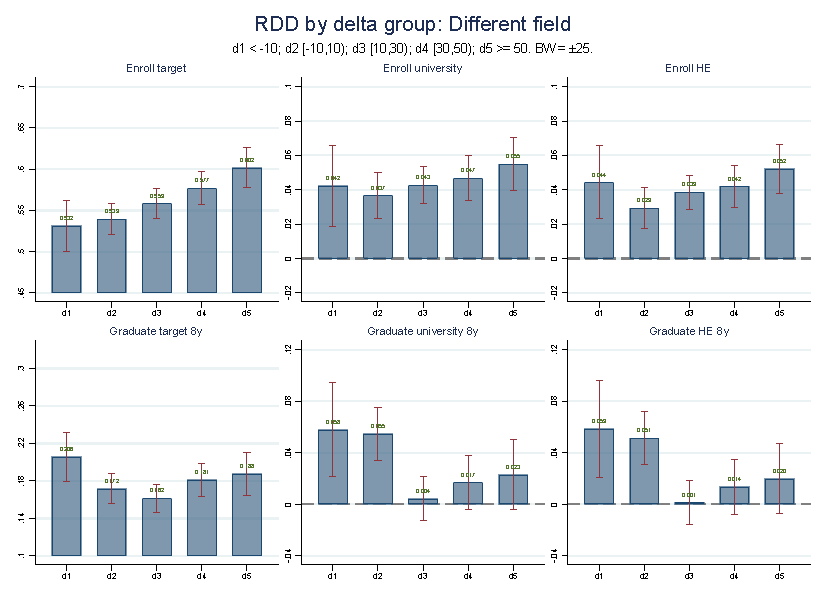
\includegraphics[width=0.7\textwidth]{../../output/figures/same_field_nextbest/rdd_delta_different_field_8y.pdf}

\vskip 0.1cm

\tiny
\begin{itemize}
\item Within different-field alternatives, target-enrollment effects also increase with the selectivity gap.

\item Broader graduation effects are less stable across groups, suggesting more heterogeneous substitution patterns when the fallback option is in another field.
\end{itemize}
\end{frame}


%====================================================
\section{Inframarginal Program-Year Analysis}
%====================================================
\begin{frame}{From Marginal to Inframarginal Students}

\small

\begin{itemize}

\item The previous analysis focused on applicants located around admission cutoffs.

\item We now study \textbf{inframarginal students}: applicants who would have been admitted to their target program in every year of the relevant period.

\item To identify them, we reconstruct each student's application score using the admission weights from each year and compare it with the corresponding admission cutoff.

\item The objective is to estimate whether changes in program capacity affect the outcomes of these inframarginal cohorts.

\end{itemize}
\end{frame}

%----------------------------------------------------
\subsection{Inframarginal Design No. 1}
\begin{frame}{Inframarginal Design}


\textbf{Specification}

\begin{itemize}
    \item Following the model notes, program size should be measured using \emph{total enrollment}:
    \[
    \Delta N^{total}_{pt}
    =
    \pi \Delta Z_{pt}
    +
    \alpha_t
    +
    \nu_{pt}.
    \]

    \item Outcomes continue to be computed using inframarginal students:
    \[
    \Delta y^{infra}_{pt}
    =
    \beta \widehat{\Delta N}^{total}_{pt}
    +
    \alpha_t
    +
    \varepsilon_{pt}.
    \]
\end{itemize} 

\vspace{0.15cm}
\begin{itemize}
    \item $N_{pt}^{total}$: total enrollment in program $p$ and year $t$.
    \item $Z_{pt}$: total vacancies/cupos.
    \item $y_{pt}^{infra}$: graduation rate among inframarginal students.
\end{itemize}



\end{frame}




\begin{frame}{Corrected Inframarginal IV Results}

\centering
\tiny

\begin{tabular}{lllcccc}
\toprule
Period & Instrument & Outcome & First stage & F-stat & Reduced form & 2SLS \\
\midrule

2007--2012 & $\Delta$ Total Cupos & Target grad. 8y
& 0.816 & 482.57 & -0.00038 & -0.00048 \\
& & 
& (0.037) &  & (0.00024) & (0.00030) \\

2007--2012 & $\Delta$ Total Cupos & Univ. grad. 8y
& 0.816 & 482.57 & 0.00063 & 0.00079** \\
& &
& (0.037) &  & (0.00030) & (0.00035) \\

2007--2012 & $\Delta$ Total Cupos & HE grad. 8y
& 0.816 & 482.57 & 0.00063 & 0.00079** \\
& &
& (0.037) &  & (0.00030) & (0.00035) \\

\midrule


2013--2016 & $\Delta$ Total Cupos & Target grad. 8y
& 0.543 & 96.11 & -0.00011 & -0.00020 \\
& &
& (0.054) &  & (0.00034) & (0.00064) \\

2013--2016 & $\Delta$ Total Cupos & Univ. grad. 8y
& 0.543 & 96.11 & 0.00048* & 0.00088** \\
& &
& (0.054) &  & (0.00025) & (0.00039) \\

2013--2016 & $\Delta$ Total Cupos & HE grad. 8y
& 0.543 & 96.11 & 0.00048* & 0.00088** \\
& &
& (0.054) &  & (0.00025) & (0.00039) \\

\bottomrule
\end{tabular}

\vspace{0.08cm}

\tiny
Standard errors in parentheses. First stage: $\Delta N^{total}_{pt}$ on $\Delta Z_{pt}$.
Reduced form: $\Delta y^{infra}_{pt}$ on $\Delta Z_{pt}$.
2SLS: $\Delta y^{infra}_{pt}$ on predicted $\Delta N^{total}_{pt}$.
$^{*}p<0.10$, $^{**}p<0.05$, $^{***}p<0.01$.

\end{frame}




\begin{frame}{First Stage Robustness and Residual Variation}

\centering
\tiny 
\textbf{Panel A. Sequential first-stage specifications}

\vspace{0.05cm}



\begin{tabular}{lcc}
\toprule
Specification & 2007--2012 & 2013--2016 \\
\midrule
Differences, no FE & 0.817 & 0.543 \\
Differences + year FE & 0.816 & 0.543 \\
Differences + program FE & 0.816 & 0.637 \\
Differences + program + year FE & 0.813 & 0.638 \\
Levels + program + year FE & 0.824 & 0.525 \\
\bottomrule
\end{tabular}

\vspace{0.25cm}

\textbf{Panel B. Residual variation after program and year FE}

\vspace{0.05cm}

\begin{tabular}{lcccc}
\toprule
Period 
& Enrollment SD
& Residual enrollment SD
& Cupos SD
& Residual Cupos SD \\
\midrule
2007--2012 & 45.5 & 31.8 & 49.6 & 33.5 \\
2013--2016 & 62.4 & 37.9 & 67.7 & 40.0 \\
\bottomrule
\end{tabular}

\vspace{0.2cm}

\scriptsize
\begin{itemize}
\item Adding fixed effects does not eliminate the first stage.
\item Residual variation remains substantial in both periods.
\item The weaker 2013--2016 first stage does not appear to be driven by a lack of within-program variation.
\end{itemize}

\end{frame}


%------------------------------------------------
\begin{frame}{Inframarginal Student Definitions}

Identify students who would have enrolled in the target program regardless of small changes in annual admission capacity.


\textbf{Construction}

\begin{itemize}
    \item For each program, compute the annual number of students who actually enrolled.
    \item Define an enrollment threshold using one of two alternative rules:
    \begin{itemize}
        \item \textbf{First Cohort:} size of the first observed enrolled cohort.
        \item \textbf{Minimum Cohort:} minimum enrolled cohort observed over the sample period.
    \end{itemize}
    \item An applicant is classified as inframarginal if their admission rank is at or above the threshold defined for that program.
\end{itemize}

\[
\text{Inframarginal}_{ipt}=1
\quad \Longleftrightarrow \quad
Rank_{ipt}\leq T_p,
\]

where $T_p$ is either the first enrolled cohort size or the minimum enrolled cohort size for program $p$.
\end{frame}


\begin{frame}{Results}

\scriptsize
\centering

\begin{tabular}{lcccc}
\toprule
& \shortstack{First\\Cohort}
& \shortstack{80\% First\\Cohort}
& \shortstack{Minimum\\Cohort}
& \shortstack{80\% Minimum\\Cohort} \\
\midrule

Infra students (N)
& 388,867
& 314,482
& 354,631
& 284,126 \\

Share ranked infra (\%)
& 72.90 & 58.96 & 66.48 & 53.27 \\

FD observations
& 6,523 & 6,523 & 6,521 & 6,519 \\

Programs
& 1,257 & 1,257 & 1,257 & 1,257 \\

First stage
& 0.7317*** & 0.7317*** & 0.7317*** & 0.7317*** \\
& (0.0504) & (0.0504) & (0.0504) & (0.0504) \\

F-stat
& 210.7 & 210.7 & 210.6 & 210.6 \\

2SLS Program
& 0.00009 & 0.00011 & 0.00018 & 0.00019 \\
& (0.00022) & (0.00023) & (0.00027) & (0.00029) \\

\bottomrule
\end{tabular}

\vspace{0.15cm}

\raggedright
\tiny
\textit{Notes:} Columns differ only in the definition of inframarginal students. In all columns, the threshold used to define inframarginal status is based on effective enrollment. \textbf{First Cohort} defines inframarginal students as applicants whose admission rank is weakly below the number of students effectively enrolled in the first observed cohort of each program. \textbf{80\% First Cohort} restricts this threshold to 80 percent of the first enrolled cohort. \textbf{Minimum Cohort} uses the minimum annual effective enrollment observed for each program over the sample period. \textbf{80\% Minimum Cohort} restricts this minimum threshold to 80 percent. The first stage instruments annual changes in total program enrollment with annual changes in total vacancies. The outcome is graduation from the program in which the student initially enrolled within eight years. Robust standard errors clustered at the program level are reported in parentheses.

\end{frame}


\begin{frame}{Alternative inframarginal}

\tiny
\centering

\begin{tabular}{lcccccc}
\toprule
Definition & N & Share (\%) & FD Obs. & First stage & F-stat & 2SLS \\
\midrule

\multicolumn{7}{l}{\textit{First Cohort}} \\

100\% & 388,867 & 70.59 & 6,523 & 0.7317*** & 210.7 & 0.00009 \\
      &         &       &       & (0.0504) &       & (0.00022) \\

90\% & 350,913 & 63.70 & 6,523 & 0.7317*** & 210.7 & 0.00011 \\
     &         &       &       & (0.0504) &       & (0.00023) \\

80\% & 314,482 & 57.09 & 6,523 & 0.7317*** & 210.7 & 0.00011 \\
     &         &       &       & (0.0504) &       & (0.00023) \\

70\% & 276,422 & 50.18 & 6,521 & 0.7317*** & 210.7 & 0.00009 \\
     &         &       &       & (0.0504) &       & (0.00023) \\

60\% & 238,522 & 43.30 & 6,519 & 0.7317*** & 210.7 & 0.00009 \\
     &         &       &       & (0.0504) &       & (0.00024) \\

\midrule

\multicolumn{7}{l}{\textit{Minimum Cohort}} \\

100\% & 354,631 & 64.37 & 6,521 & 0.7317*** & 210.6 & 0.00018 \\
      &         &       &       & (0.0504) &       & (0.00027) \\

90\% & 318,091 & 57.74 & 6,519 & 0.7317*** & 210.6 & 0.00021 \\
     &         &       &       & (0.0504) &       & (0.00028) \\

80\% & 284,126 & 51.58 & 6,519 & 0.7317*** & 210.6 & 0.00019 \\
     &         &       &       & (0.0504) &       & (0.00029) \\

70\% & 249,085 & 45.21 & 6,513 & 0.7317*** & 210.6 & 0.00014 \\
     &         &       &       & (0.0504) &       & (0.00029) \\

60\% & 214,682 & 38.97 & 6,511 & 0.7317*** & 210.6 & 0.00020 \\
     &         &       &       & (0.0504) &       & (0.00030) \\

\bottomrule
\end{tabular}

\vspace{0.12cm}

\raggedright
\tiny
\textit{Notes:} The table reports robustness checks using progressively more conservative definitions of inframarginal students. For each program, the baseline definition uses either the size of the first enrolled cohort (\textit{First Cohort}) or the minimum enrolled cohort observed over 2007--2016 (\textit{Minimum Cohort}). Alternative definitions restrict the inframarginal sample to the top 90\%, 80\%, 70\%, and 60\% of each baseline cohort size. All thresholds are based on effective enrollment and then applied to applicants according to their admission ranking. The first stage instruments annual changes in total enrollment with annual changes in total vacancies. The outcome is graduation from the initially enrolled program within eight years. Robust standard errors clustered at the program level are reported in parentheses.

\end{frame}


\begin{frame}{Heterogeneity by University Selectivity: First Cohort}

\scriptsize
\centering

\begin{tabular}{lcccc}
\toprule
University
& Mean PSU
& First stage
& F-stat
& 2SLS \\
\midrule

\multicolumn{5}{l}{\textit{More selective universities}} \\

Univ. Católica
& 685.8
& 0.9925***
& 1,284.7
& -0.00023 \\
&
&
(0.0277)
&
&
(0.00036) \\[0.06cm]

Univ. de Chile
& 675.7
& 0.8039***
& 322.6
& -0.00003 \\
&
&
(0.0448)
&
&
(0.00031) \\[0.06cm]

Univ. de Santiago
& 616.7
& 0.8508***
& 728.1
& 0.00113** \\
&
&
(0.0315)
&
&
(0.00053) \\

\midrule

\multicolumn{5}{l}{\textit{Less selective universities}} \\

Univ. Playa Ancha
& 548.4
& 0.6235***
& 131.1
& -0.01385*** \\
&
&
(0.0545)
&
&
(0.00282) \\[0.06cm]

Univ. Católica de Concepción
& 558.0
& 0.4448***
& 74.3
& 0.00005 \\
&
&
(0.0516)
&
&
(0.00260) \\[0.06cm]

Univ. del Bío-Bío
& 560.5
& 0.6681***
& 12.2
& -0.01598** \\
&
&
(0.1913)
&
&
(0.00797) \\

\bottomrule
\end{tabular}

\vspace{0.18cm}

\raggedright
\tiny
\textit{Notes:} Results use the 2007--2016 panel and the \textit{First Cohort}
definition of inframarginal students. Mean PSU is the average
Language--Mathematics PSU score of students enrolled in their target program.
The first stage estimates the effect of annual changes in total vacancies on
annual changes in total program enrollment. The 2SLS coefficient estimates the
effect of one additional enrolled student induced by changes in vacancies on
the eight-year graduation rate from the initially enrolled program among
inframarginal students. Robust standard errors clustered at the program level
are reported in parentheses. $^{*}p<0.10$, $^{**}p<0.05$,
$^{***}p<0.01$.

\end{frame}

\begin{frame}{Heterogeneity by University Selectivity: Minimum Cohort}

\scriptsize
\centering

\begin{tabular}{lcccc}
\toprule
University
& Mean PSU
& First stage
& F-stat
& 2SLS \\
\midrule

\multicolumn{5}{l}{\textit{More selective universities}} \\

Univ. Católica
& 685.8
& 0.9925***
& 1,284.7
& -0.00023 \\
&
&
(0.0277)
&
&
(0.00037) \\[0.06cm]

Univ. de Chile
& 675.7
& 0.8039***
& 322.6
& -0.00008 \\
&
&
(0.0448)
&
&
(0.00031) \\[0.06cm]

Univ. de Santiago
& 616.7
& 0.8508***
& 728.1
& 0.00113** \\
&
&
(0.0315)
&
&
(0.00053) \\

\midrule

\multicolumn{5}{l}{\textit{Less selective universities}} \\

Univ. Playa Ancha
& 548.4
& 0.6235***
& 131.1
& -0.01447*** \\
&
&
(0.0545)
&
&
(0.00293) \\[0.06cm]

Univ. Católica de Concepción
& 558.0
& 0.4448***
& 74.3
& 0.00007 \\
&
&
(0.0516)
&
&
(0.00285) \\[0.06cm]

Univ. del Bío-Bío
& 560.5
& 0.6681***
& 12.2
& -0.01756** \\
&
&
(0.1913)
&
&
(0.00837) \\

\bottomrule
\end{tabular}

\vspace{0.18cm}

\raggedright
\tiny
\textit{Notes:} Results use the 2007--2016 panel and the \textit{Minimum Cohort}
definition of inframarginal students. Mean PSU is the average
Language--Mathematics PSU score of students enrolled in their target program.
The first stage estimates the effect of annual changes in total vacancies on
annual changes in total program enrollment. The 2SLS coefficient estimates the
effect of one additional enrolled student induced by changes in vacancies on
the eight-year graduation rate from the initially enrolled program among
inframarginal students. Robust standard errors clustered at the program level
are reported in parentheses. $^{*}p<0.10$, $^{**}p<0.05$,
$^{***}p<0.01$.

\end{frame}

\begin{frame}{Program selectivity and graduation effects}

\tiny
\centering

\textbf{Panel A. First Cohort}

\vspace{0.05cm}

\begin{tabular}{lccccc}
\toprule
Program selectivity & Programs & FD obs. & First Stage & F-stat & 2SLS \\
\midrule
PSU $<550$
    & 410 & 1,400 & 0.4356*** & 217.0 & 0.00125 \\
    &&& (0.0296) && (0.00112) \\

PSU 550--600
    & 467 & 2,563 & 0.5165*** & 196.3 & 0.00036 \\
    &&& (0.0369) && (0.00071) \\

PSU 600--650
    & 249 & 1,665 & 0.7510*** & 238.9 & -0.00032 \\
    &&& (0.0486) && (0.00053) \\

PSU $\geq650$
    & 131 & 895 & 0.9229*** & 802.3 & -0.00009 \\
    &&& (0.0326) && (0.00018) \\
\bottomrule
\end{tabular}

\vspace{0.35cm}

\textbf{Panel B. Minimum Cohort}

\vspace{0.05cm}

\begin{tabular}{lccccc}
\toprule
Program selectivity & Programs & FD obs. & First Stage & F-stat & 2SLS \\
\midrule
PSU $<550$
    & 410 & 1,400 & 0.4356*** & 217.0 & 0.00140 \\
    &&& (0.0296) && (0.00117) \\

PSU 550--600
    & 467 & 2,561 & 0.5162*** & 196.0 & 0.00048 \\
    &&& (0.0369) && (0.00077) \\

PSU 600--650
    & 249 & 1,665 & 0.7510*** & 238.9 & -0.00023 \\
    &&& (0.0486) && (0.00052) \\

PSU $\geq650$
    & 131 & 895 & 0.9229*** & 802.3 & -0.00004 \\
    &&& (0.0326) && (0.00025) \\
\bottomrule
\end{tabular}

\vspace{0.15cm}

\raggedright
\tiny
Notes: Programs are classified according to the average Language--Mathematics PSU score of enrolled students over 2007--2016:
PSU $<550$, 550--600, 600--650, and PSU $\geq650$.
Standard errors clustered at the program level are reported in parentheses.
Outcomes correspond to graduation from the initially enrolled program within eight years.

\end{frame}



\begin{frame}{Heterogeneity by Field of Study}

\tiny
\centering

\begin{tabular}{lccccc}
\toprule
Field group & Programs & FD obs. & First stage & F-stat & 2SLS \\
\midrule

\multicolumn{6}{l}{\textbf{Panel A. First Cohort}} \\

Business and Law
& 130 & 651 & 0.6305*** & 93.0 & 0.00179** \\
&&& (0.0654) && (0.00084) \\

Health
& 221 & 1,290 & 0.4074*** & 142.1 & -0.00013 \\
&&& (0.0342) && (0.00082) \\

STEM
& 432 & 2,162 & 0.8502*** & 320.7 & -0.00015 \\
&&& (0.0475) && (0.00010) \\

Education and Humanities
& 372 & 1,913 & 0.7158*** & 51.9 & -0.00060 \\
&&& (0.0994) && (0.00061) \\

Arts, Architecture and Agriculture
& 102 & 507 & 0.6541*** & 138.0 & 0.00070 \\
&&& (0.0557) && (0.00120) \\

\midrule

\multicolumn{6}{l}{\textbf{Panel B. Minimum Cohort}} \\

Business and Law
& 130 & 651 & 0.6305*** & 93.0 & 0.00189** \\
&&& (0.0654) && (0.00084) \\

Health
& 221 & 1,288 & 0.4069*** & 141.9 & 0.00013 \\
&&& (0.0342) && (0.00084) \\

STEM
& 432 & 2,162 & 0.8502*** & 320.7 & -0.00014 \\
&&& (0.0475) && (0.00012) \\

Education and Humanities
& 372 & 1,913 & 0.7158*** & 51.9 & -0.00062 \\
&&& (0.0994) && (0.00064) \\

Arts, Architecture and Agriculture
& 102 & 507 & 0.6541*** & 138.0 & 0.00073 \\
&&& (0.0557) && (0.00117) \\

\bottomrule
\end{tabular}

\vspace{0.10cm}

\raggedright
\tiny
\textit{Notes:} Results use the 2007--2016 panel. Fields are grouped using the target program's field of study and fixed at the program level. The first stage estimates the effect of annual changes in vacancies on annual changes in total enrollment. The 2SLS coefficient estimates the effect of one additional enrolled student, induced by changes in vacancies, on the eight-year graduation rate from the initially enrolled program among inframarginal students. Robust standard errors clustered at the program level are reported in parentheses. $^{*}p<0.10$, $^{**}p<0.05$, $^{***}p<0.01$.

\end{frame}



\begin{frame}{Inframarginal Students: Graduation at 8 vs. 10 Years}

\scriptsize
\centering

\begin{tabular}{lccccc}
\toprule
Definition & Horizon & Programs & FD obs. & First stage & 2SLS \\
\midrule

First Cohort
& 8 years
& 1,092
& 4,881
& 0.7413***
& 0.00002 \\
&&&& (0.0579) & (0.00021) \\[0.05cm]

First Cohort
& 10 years
& 1,092
& 4,881
& 0.7413***
& 0.00031 \\
&&&& (0.0579) & (0.00034) \\[0.05cm]

Minimum Cohort
& 8 years
& 1,092
& 4,881
& 0.7413***
& 0.00010 \\
&&&& (0.0579) & (0.00027) \\[0.05cm]

Minimum Cohort
& 10 years
& 1,092
& 4,881
& 0.7413***
& 0.00048 \\
&&&& (0.0579) & (0.00043) \\

\bottomrule
\end{tabular}

\vspace{0.15cm}

\raggedright
\tiny
\textit{Notes:} The table compares graduation outcomes measured within eight and ten years using the same 2007--2014 sample. The outcome is graduation from the program in which the student initially enrolled. Each estimate uses 1,092 programs and 4,881 first-difference observations. The first stage instruments annual changes in total program enrollment with annual changes in total vacancies; the first-stage coefficient implies that 10 additional vacancies increase enrollment by approximately 7.4 students. Robust standard errors clustered at the program level are reported in parentheses. $^{*}p<0.10$, $^{**}p<0.05$, $^{***}p<0.01$.
\end{frame}

%------------------------------------------------
\begin{frame}{Inframarginal IV results}

\scriptsize

\begin{center}
\begin{tabular}{lcccc}
\toprule
Outcome & First stage & F-stat & Reduced form & 2SLS \\
\midrule

Target graduation, 8y
& 0.732
& 210.7
& 0.00013
& 0.00019 \\
&
(0.050)
&
&
(0.00020)
&
(0.00028) \\

University graduation, 8y
& 0.732
& 210.7
& 0.00005
& 0.00007 \\
&
(0.050)
&
&
(0.00012)
&
(0.00016) \\

Higher education graduation, 8y
& 0.732
& 210.7
& 0.00005
& 0.00007 \\
&
(0.050)
&
&
(0.00012)
&
(0.00016) \\

\bottomrule
\end{tabular}
\end{center}

\vspace{0.2cm}

\begin{itemize}
    \item 494,675 inframarginal students (90.6\% of enrollment).
\end{itemize}

\end{frame}

%------------------------------------------------
\begin{frame}{Heterogeneity by university selectivity}

\scriptsize

\begin{center}
\begin{tabular}{lccccc}
\toprule
University &
Mean PSU &
First stage &
F-stat &
Reduced form &
2SLS \\
\midrule

\multicolumn{6}{l}{\textit{Highly selective universities}} \\

UC
& 693.1
& 0.993
& 903.9
& 0.00024
& 0.00024 \\
&
&
(0.028)
&
&
(0.00028)
&
(0.00028) \\

UCH
& 686.1
& 0.804
& 390.5
& 0.00096***
& 0.00119*** \\
&
&
(0.045)
&
&
(0.00026)
&
(0.00036) \\

\midrule

\multicolumn{6}{l}{\textit{Less selective universities}} \\

UNAB
& 559.2
& 0.380
& 90.8
& -0.00029
& -0.00076 \\
&
&
(0.040)
&
&
(0.00022)
&
(0.00060) \\

UCSC
& 563.5
& 0.445
& 75.4
& -0.00174**
& -0.00385** \\
&
&
(0.052)
&
&
(0.00076)
&
(0.00157) \\

UBB
& 567.5
& 0.668
& 14.1
& -0.00464**
& -0.00673* \\
&
&
(0.191)
&
&
(0.00206)
&
(0.00366) \\

\bottomrule
\end{tabular}
\end{center}

\vspace{0.15cm}

\tiny
\begin{itemize}
    \item Mean PSU is based on target-program selectivity.
    \item Outcome: university graduation among inframarginal students.
    \item Negative effects emerge mainly among less selective institutions.
\end{itemize}

\end{frame}


\subsection{Inframarginal Design No. 2}
%=========================================================
% DESIGN II: OWN SUDDEN VACANCY EXPANSIONS (issue #3)
%=========================================================
\begin{frame}{Design II: what happens when a selective program expands its seats?}
\scriptsize
\textbf{Research question}

When a selective program suddenly increases its regular-admission vacancies, what happens to
(a) its own first-year enrollment, (b) the composition of its entering cohort, and
(c) the outcomes of its inframarginal students?

\vspace{0.10cm}
\textbf{Approach}
\begin{itemize}
    \item A simple DiD built on Design I, but with a \emph{binary} treatment: a large, sudden own expansion.
    \item Design I uses every year-to-year change in vacancies, most of which are small and routine.
    Here, identification comes from discrete capacity decisions, and the event study makes pre-trends testable.
    \item The shock is the program's own decision, so it is not exogenous to its demand. Leads in the event study are the main diagnostic.
\end{itemize}

\vspace{0.06cm}
\textbf{Sample}
\begin{itemize}
    \item Incumbent program $\times$ admission-year panel, 2007--2016 (programs with 2007--2009 entrants; SUA entrants excluded): 796 programs.
    \item \textbf{Selective programs}: top 20\% of 2007--2009 mean entrant PSU (predetermined; cutoff 633.6 points). 169 programs.
\end{itemize}
\end{frame}

%--------------------------------------------------------
\begin{frame}{Design II: distribution of vacancy changes, selective programs}
\centering
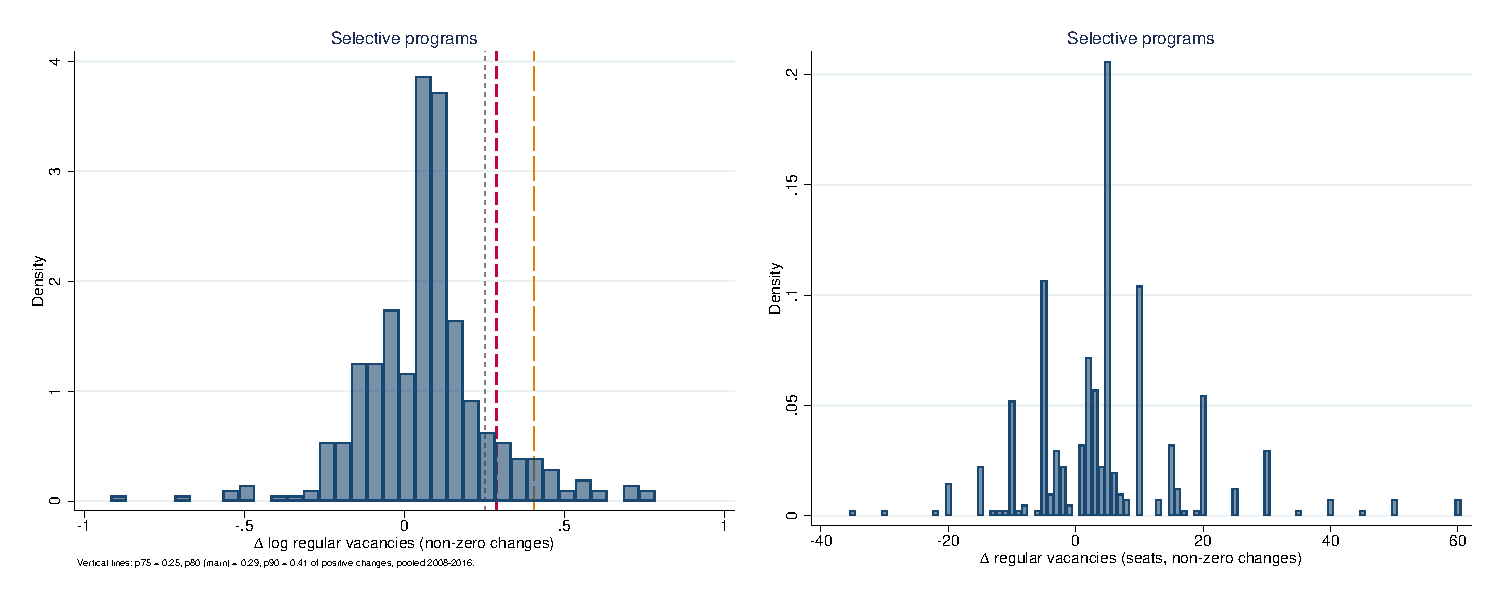
\includegraphics[width=0.85\textwidth, height=0.36\textheight, keepaspectratio]{../../output/own_expansion/figures/oe_dV_hist_sel.pdf}

\vspace{0.05cm}
\tiny
\resizebox{0.78\textwidth}{!}{\begin{tabular}{lcccccc}
\toprule
 & & & \multicolumn{2}{c}{Shocks, 2010--2016} & \multicolumn{2}{c}{Programs ever treated} \\
\cmidrule(lr){4-5}\cmidrule(lr){6-7}
Definition & \(\Delta\log V\) threshold & Increase & All & Selective & All & Selective \\
\midrule
Top 25\% & 0.251 & + 29\% &  183 &   41 &  141 &   27 \\
Top 20\% (main) & 0.288 & + 33\% &  159 &   33 &  119 &   20 \\
Top 10\% & 0.405 & + 50\% &   73 &   16 &   58 &   10 \\
\midrule
Programs in sample & & & & &  796 &  169 \\
\bottomrule
\end{tabular}
}

\vspace{0.05cm}
\begin{itemize}\scriptsize
    \setlength{\itemsep}{0pt}
    \item \textbf{Large change} = Design IV shock: top 20\% of positive $\Delta\log V$ ($\ge +33\%$; many increases sit exactly there) and sudden.
    \item Only 20 selective programs are ever treated. The top 25\% and top 10\% thresholds serve as robustness checks.
\end{itemize}
\end{frame}

%--------------------------------------------------------
\begin{frame}{Design II: construction of variables and models}
\scriptsize
\setlength{\abovedisplayskip}{2pt}
\setlength{\belowdisplayskip}{2pt}
\textbf{Treatment}
\begin{itemize}
    \item $\text{shock}_{pt}=1$ if $\Delta\log V_{pt}$ is in the top 20\% of positive changes, $V_{p,t-2}$ is observed, $p$ was not shocked in $t-1$,
    and the increase is not reversed in $t+1$. Shocks are dated 2010--2016 (identical to Design IV's source shocks).
    \item $g_p$: first shock year (staggered). $\text{Post}_{pt}=\mathbf 1\{t\ge g_p\}$, absorbing.
\end{itemize}

\textbf{Outcomes}: regular vacancies $V_{pt}$ (mechanical check), first-year enrollment $N_{pt}$ (Formulario D), and composition of entrants.

\vspace{0.08cm}
\textbf{(1) TWFE}
\[
y_{pt}=\beta\,\text{Post}_{pt}+\mu_p+\alpha_{f(p),t}+\gamma_{r(p),t}+\varepsilon_{pt}
\]
\textbf{(2) Event study}
\[
y_{pt}=\sum_{\ell\neq-1}b_\ell\,\mathbf 1\{t-g_p=\ell\}+\mu_p+\alpha_{f(p),t}+\gamma_{r(p),t}+e_{pt},\qquad \ell\in\{\le-5,\dots,\ge4\}
\]
\textbf{(3) Callaway \& Sant'Anna}: never treated only, and not yet treated plus never treated. Balanced panel.

\vspace{0.05cm}
\begin{itemize}
    \item SE clustered by program. Specification (1) in the tables also includes a version with program and year FE only.
    \item Inframarginal outcome (graduation of inframarginal students): \textbf{pending}. The Design I rank file
    (\texttt{admission\_rank\_inframarginal\_2007\_2016.dta}) has no builder in the repository.
\end{itemize}
\end{frame}

%--------------------------------------------------------
\begin{frame}{Design II: results, own enrollment}
\centering
\tiny
\resizebox{0.80\textwidth}{!}{\begin{tabular}{lcccccc}
\toprule
 & \multicolumn{4}{c}{Selective programs} & \multicolumn{2}{c}{All programs} \\
\cmidrule(lr){2-5}\cmidrule(lr){6-7}
 & TWFE & TWFE & CS & CS & TWFE & TWFE \\
 & (1) & (2) & never & not yet & (1) & (2) \\
\midrule
Regular vacancies &  24.237\sym{***} &  20.766\sym{***} &  22.784\sym{***} &  22.818\sym{***} &  18.196\sym{***} &  16.911\sym{***} \\
 & ( 4.337) & ( 4.138) & ( 4.219) & ( 4.217) & ( 1.573) & ( 1.593) \\
\quad \textit{Pre-mean treated; N} & \multicolumn{4}{c}{\scriptsize  49.87; 1,883} & \multicolumn{2}{c}{\scriptsize  40.37; 8,915} \\
\addlinespace
First-year enrollment (Formulario D) &  22.215\sym{***} &  18.069\sym{***} &  19.541\sym{***} &  19.592\sym{***} &  14.565\sym{***} &  13.668\sym{***} \\
 & ( 4.422) & ( 4.180) & ( 4.792) & ( 4.829) & ( 1.767) & ( 1.691) \\
\quad \textit{Pre-mean treated; N} & \multicolumn{4}{c}{\scriptsize  54.54; 1,883} & \multicolumn{2}{c}{\scriptsize  42.55; 8,915} \\
\addlinespace
Log first-year enrollment &   0.370\sym{***} &   0.342\sym{***} &   0.276\sym{***} &   0.275\sym{***} &   0.275\sym{***} &   0.256\sym{***} \\
 & ( 0.049) & ( 0.050) & ( 0.039) & ( 0.039) & ( 0.040) & ( 0.037) \\
\quad \textit{Pre-mean treated; N} & \multicolumn{4}{c}{\scriptsize   3.91; 1,882} & \multicolumn{2}{c}{\scriptsize   3.54; 8,865} \\
\addlinespace
\bottomrule
\end{tabular}
}

\vspace{0.05cm}
\begin{columns}[T,onlytextwidth]
\begin{column}{0.48\textwidth}
\centering
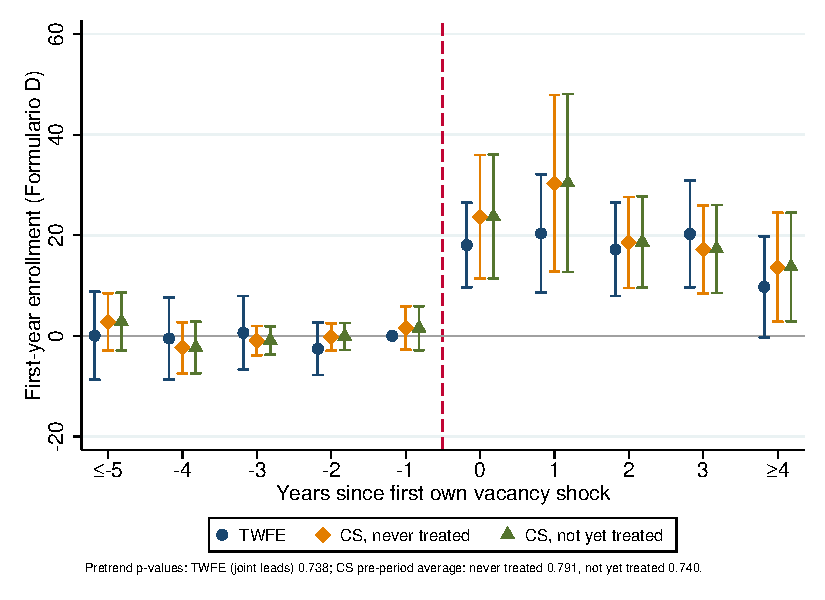
\includegraphics[width=\linewidth, height=0.36\textheight, keepaspectratio]{../../output/own_expansion/figures/oe_es_N_first_sel.pdf}
\end{column}
\begin{column}{0.48\textwidth}
\centering
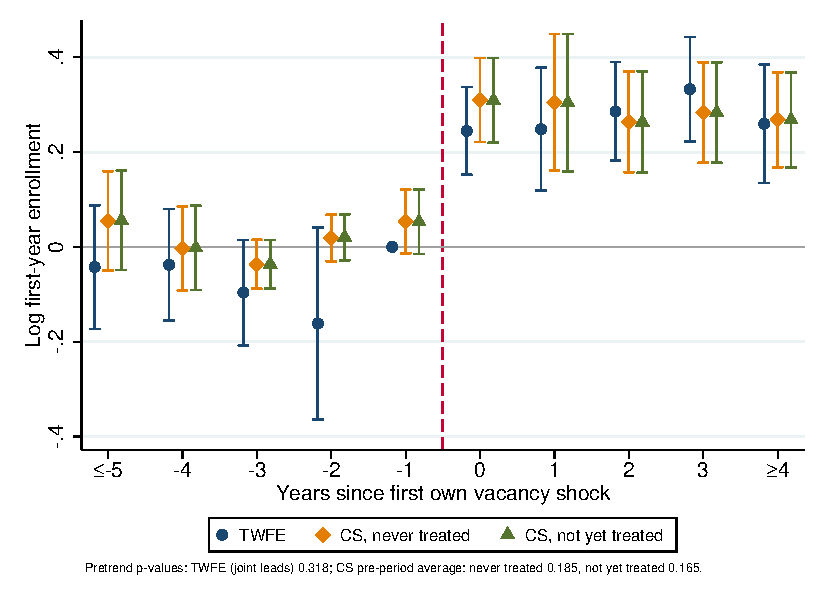
\includegraphics[width=\linewidth, height=0.36\textheight, keepaspectratio]{../../output/own_expansion/figures/oe_es_lnN_sel.pdf}
\end{column}
\end{columns}

\parbox{0.97\textwidth}{\tiny
\textit{Notes:} TWFE (1): program and year FE. TWFE (2): program, field $\times$ year and region $\times$ year FE.
CS: Callaway--Sant'Anna simple ATT. SE clustered by program. Event studies: selective programs.
\sym{***}~$p<0.01$, \sym{**}~$p<0.05$, \sym{*}~$p<0.10$.
After a sudden expansion, selective programs add about 21 seats and 18 entrants (pass-through $\approx 0.87$, $+34$ log points),
with flat leads (TWFE joint-leads $p=0.74$).}
\end{frame}

%--------------------------------------------------------
\begin{frame}{Design II: composition of the entering cohort}
\centering
\tiny
\resizebox{0.90\textwidth}{!}{\begin{tabular}{lcc}
\toprule
 & TWFE (1) & TWFE (2) \\
\midrule
Mean LM PSU, entrants &  -5.071\sym{***} &  -4.284\sym{***} \\
 & ( 1.424) & ( 1.256) \\
\quad \textit{Pre-mean treated; N} & \multicolumn{2}{c}{\scriptsize 584.11; 8,865} \\
\addlinespace
SD of LM PSU, entrants &  -0.103 &  -0.476 \\
 & ( 0.621) & ( 0.633) \\
\quad \textit{Pre-mean treated; N} & \multicolumn{2}{c}{\scriptsize  34.03; 8,726} \\
\addlinespace
Mean NEM, entrants &  -7.695\sym{***} &  -7.514\sym{***} \\
 & ( 2.175) & ( 2.252) \\
\quad \textit{Pre-mean treated; N} & \multicolumn{2}{c}{\scriptsize 598.05; 8,865} \\
\addlinespace
Female, entrants, pct. &  -0.510 &  -0.404 \\
 & ( 0.752) & ( 0.808) \\
\quad \textit{Pre-mean treated; N} & \multicolumn{2}{c}{\scriptsize  50.29; 8,865} \\
\addlinespace
Private-paid school, entrants, pct. &  -0.383 &  -0.072 \\
 & ( 0.385) & ( 0.411) \\
\quad \textit{Pre-mean treated; N} & \multicolumn{2}{c}{\scriptsize  10.97; 8,865} \\
\addlinespace
Municipal school, entrants, pct. &   1.584\sym{**} &   1.636\sym{**} \\
 & ( 0.731) & ( 0.719) \\
\quad \textit{Pre-mean treated; N} & \multicolumn{2}{c}{\scriptsize  31.12; 8,865} \\
\addlinespace
Private-paid school, last admitted, pct. &   3.453\sym{**} &   4.494\sym{**} \\
 & ( 1.628) & ( 1.774) \\
\quad \textit{Pre-mean treated; N} & \multicolumn{2}{c}{\scriptsize   9.07; 8,847} \\
\addlinespace
\bottomrule
\end{tabular}
}

\vspace{0.05cm}
\parbox{0.97\textwidth}{\tiny
\textit{Notes:} As in the previous table. Shares are in percentage points. Last admitted = lowest application score among regular admits.
Income is not available in the data (Formulario A has no income; the socioeconomic questionnaire is not in \texttt{data/}),
so school dependency is the SES proxy.}
\end{frame}

%--------------------------------------------------------
\begin{frame}{Design II: composition event studies and threshold robustness}
\begin{columns}[T,onlytextwidth]
\begin{column}{0.50\textwidth}
\centering
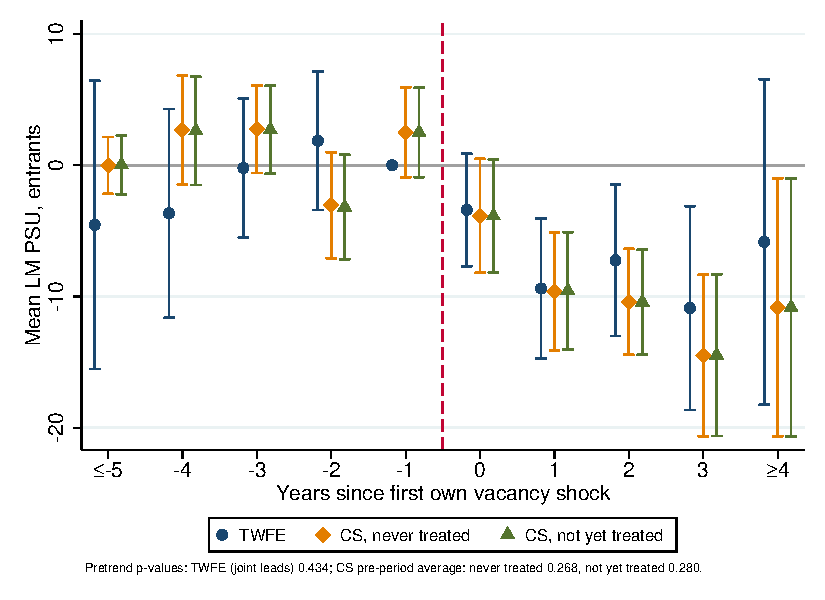
\includegraphics[width=\linewidth, height=0.40\textheight, keepaspectratio]{../../output/own_expansion/figures/oe_es_c_psu_mean_sel.pdf}

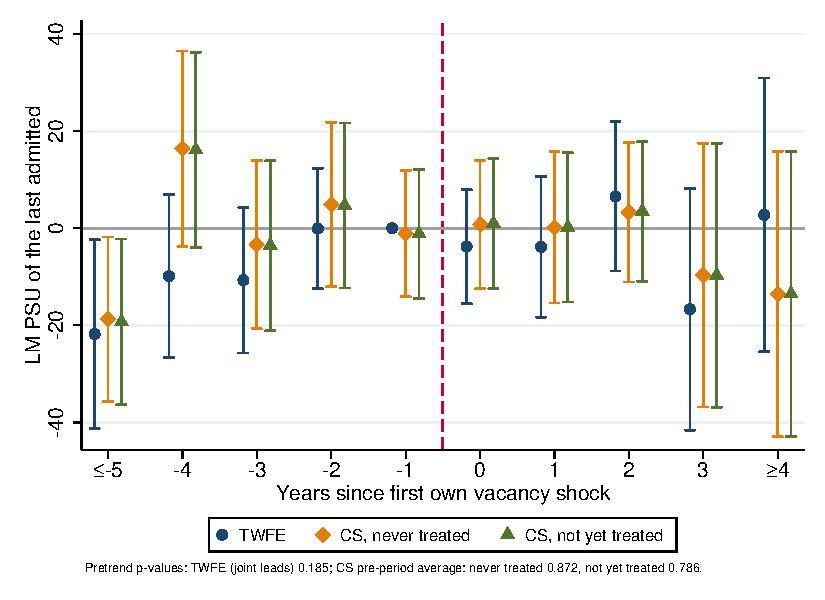
\includegraphics[width=\linewidth, height=0.40\textheight, keepaspectratio]{../../output/own_expansion/figures/oe_es_c_psu_last_sel.pdf}
\end{column}
\begin{column}{0.48\textwidth}
\centering
\tiny
\resizebox{\linewidth}{!}{\begin{tabular}{lccc}
\toprule
Outcome & Top 25\% & Top 20\% (main) & Top 10\% \\
\midrule
Regular vacancies &  29.059\sym{***} &  20.766\sym{***} &  26.995\sym{***} \\
 & ( 7.058) & ( 4.138) & ( 5.199) \\
First-year enrollment (Formulario D) &  26.414\sym{***} &  18.069\sym{***} &  22.470\sym{***} \\
 & ( 7.196) & ( 4.180) & ( 5.113) \\
Log first-year enrollment &   0.316\sym{***} &   0.342\sym{***} &   0.420\sym{***} \\
 & ( 0.041) & ( 0.050) & ( 0.077) \\
Mean LM PSU, entrants &  -8.147\sym{***} &  -6.116\sym{**} & -12.290\sym{***} \\
 & ( 2.454) & ( 2.841) & ( 3.398) \\
Private-paid school, entrants, pct. &  -0.013 &   0.338 &  -2.414 \\
 & ( 1.145) & ( 1.385) & ( 1.856) \\
\bottomrule
\end{tabular}
}

\vspace{0.2cm}
\begin{itemize}\scriptsize
    \setlength{\itemsep}{2pt}
    \item Mean entrant PSU falls by 6--9 points (about 0.15 SD of program-year means), with flat leads.
    \item The PSU of the last admitted shows no significant change, but the estimate is imprecise (SE $\approx 6$ points), so a fall of the size of the mean effect cannot be ruled out.
    \item Results are robust to the top 25\% and top 10\% shock definitions.
    \item The table uses full FE (program, field $\times$ year, region $\times$ year).
\end{itemize}
\end{column}
\end{columns}
\end{frame}

\subsection{Inframarginal Design No. 3}
%=========================================================
% SUA: ENTRY OF PRIVATE UNIVERSITIES
%========================================================
%---------------------------------------------------------
\begin{frame}{Entry of private universities into the SUA}

\footnotesize

\textbf{Research question}

Did first-year enrollment in incumbent CRUCH programs change after eight
private universities entered the SUA in 2012, particularly in programs with
greater pre-existing exposure to these entrants?

\vspace{0.10cm}

\textbf{Sample}

\begin{itemize}
    \item Incumbent CRUCH program $\times$ admission-year panel, 2007--2016.
    \item Outcome: number of students entering the first year of program $p$
    in year $t$.
\end{itemize}

\vspace{0.06cm}

\textbf{Exposure design}

\begin{itemize}
    \item Markets are defined by pre-treatment region $\times$ academic field.
    \item Exposure measures the 2009--2011 enrollment presence of the future
    entrant universities in the incumbent program's market.
    \item Total exposure uses the entrant enrollment share; Triangular and
    Gaussian measures additionally weight entrants by PSU-score proximity.
    \item Exposure is fixed over time and interacted with the post-entry
    period, 2012--2016.
\end{itemize}

\vspace{0.05cm}

\scriptsize
The design compares pre/post-2012 enrollment changes across incumbent programs
with different levels of exposure to the future entrants.

\end{frame}


%--------------------------------------------------------
%---------------------------------------------------------
%---------------------------------------------------------
\begin{frame}{Evolution of the number of SUA programs}

\begin{columns}[T,onlytextwidth]

\begin{column}{0.49\textwidth}
\centering

\textbf{\scriptsize Programs by university status}

\vspace{0.04cm}

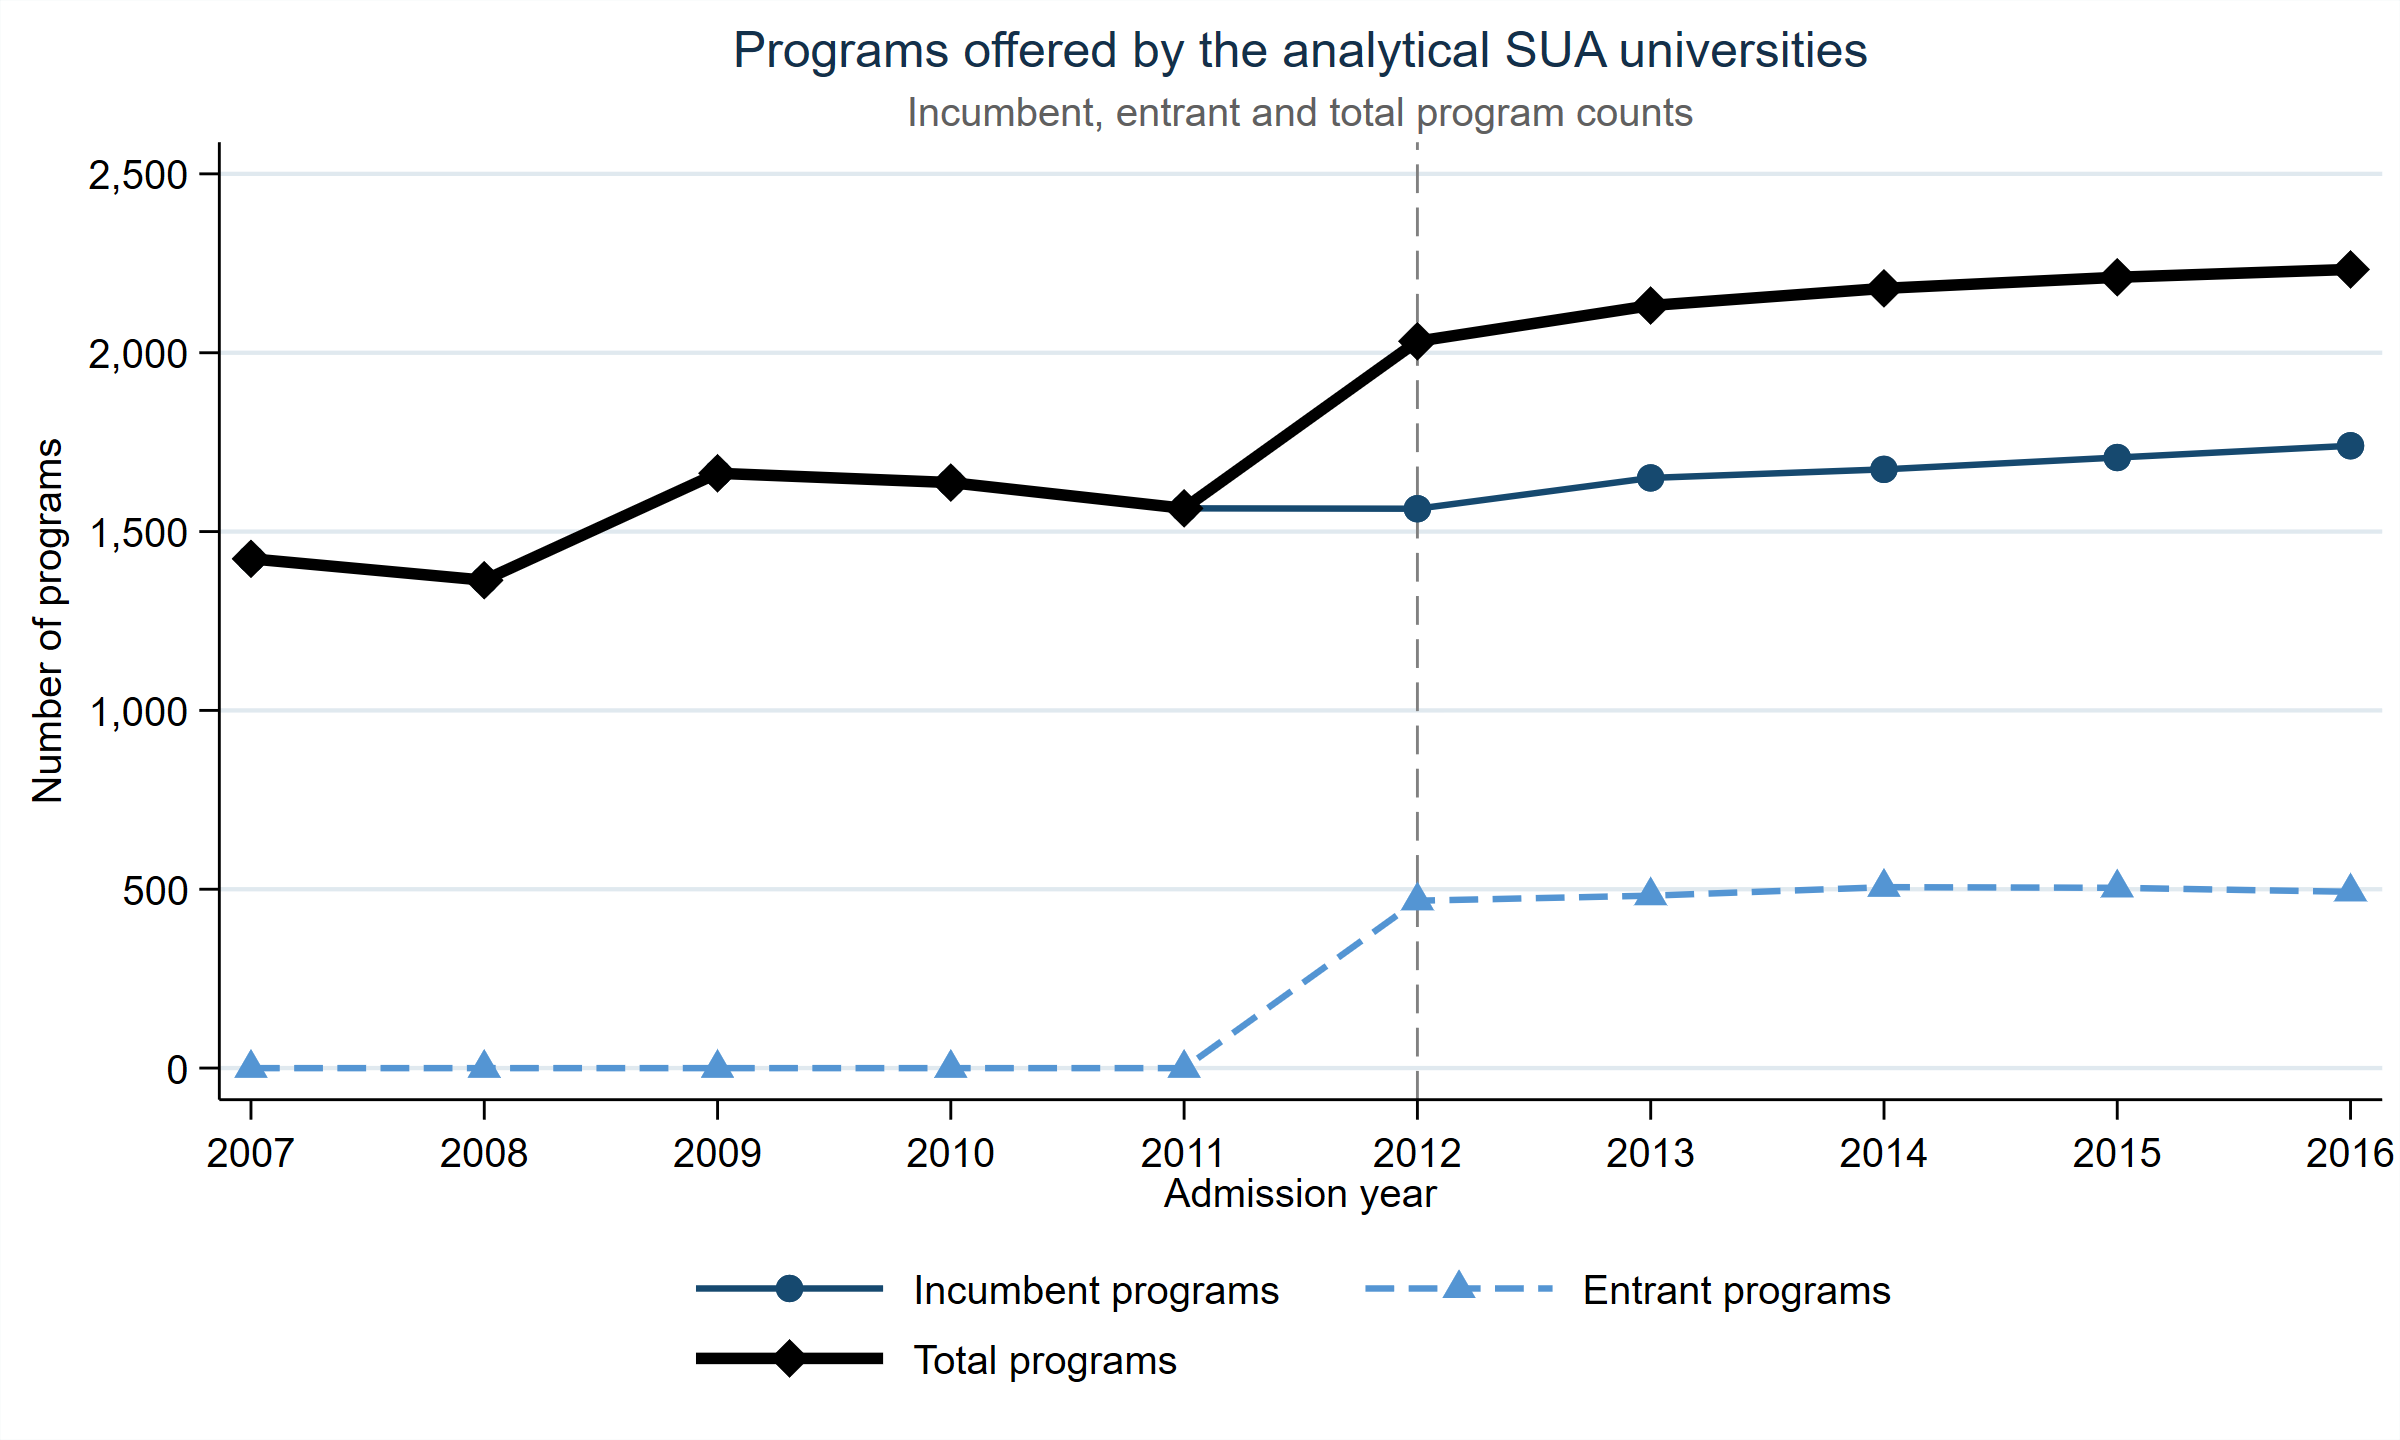
\includegraphics[ width=\linewidth ]{../../output/sua_programs_over_time_by_status.png}

\end{column}

\begin{column}{0.49\textwidth}
\centering

\textbf{\scriptsize Programs by Broad field}

\vspace{0.04cm}

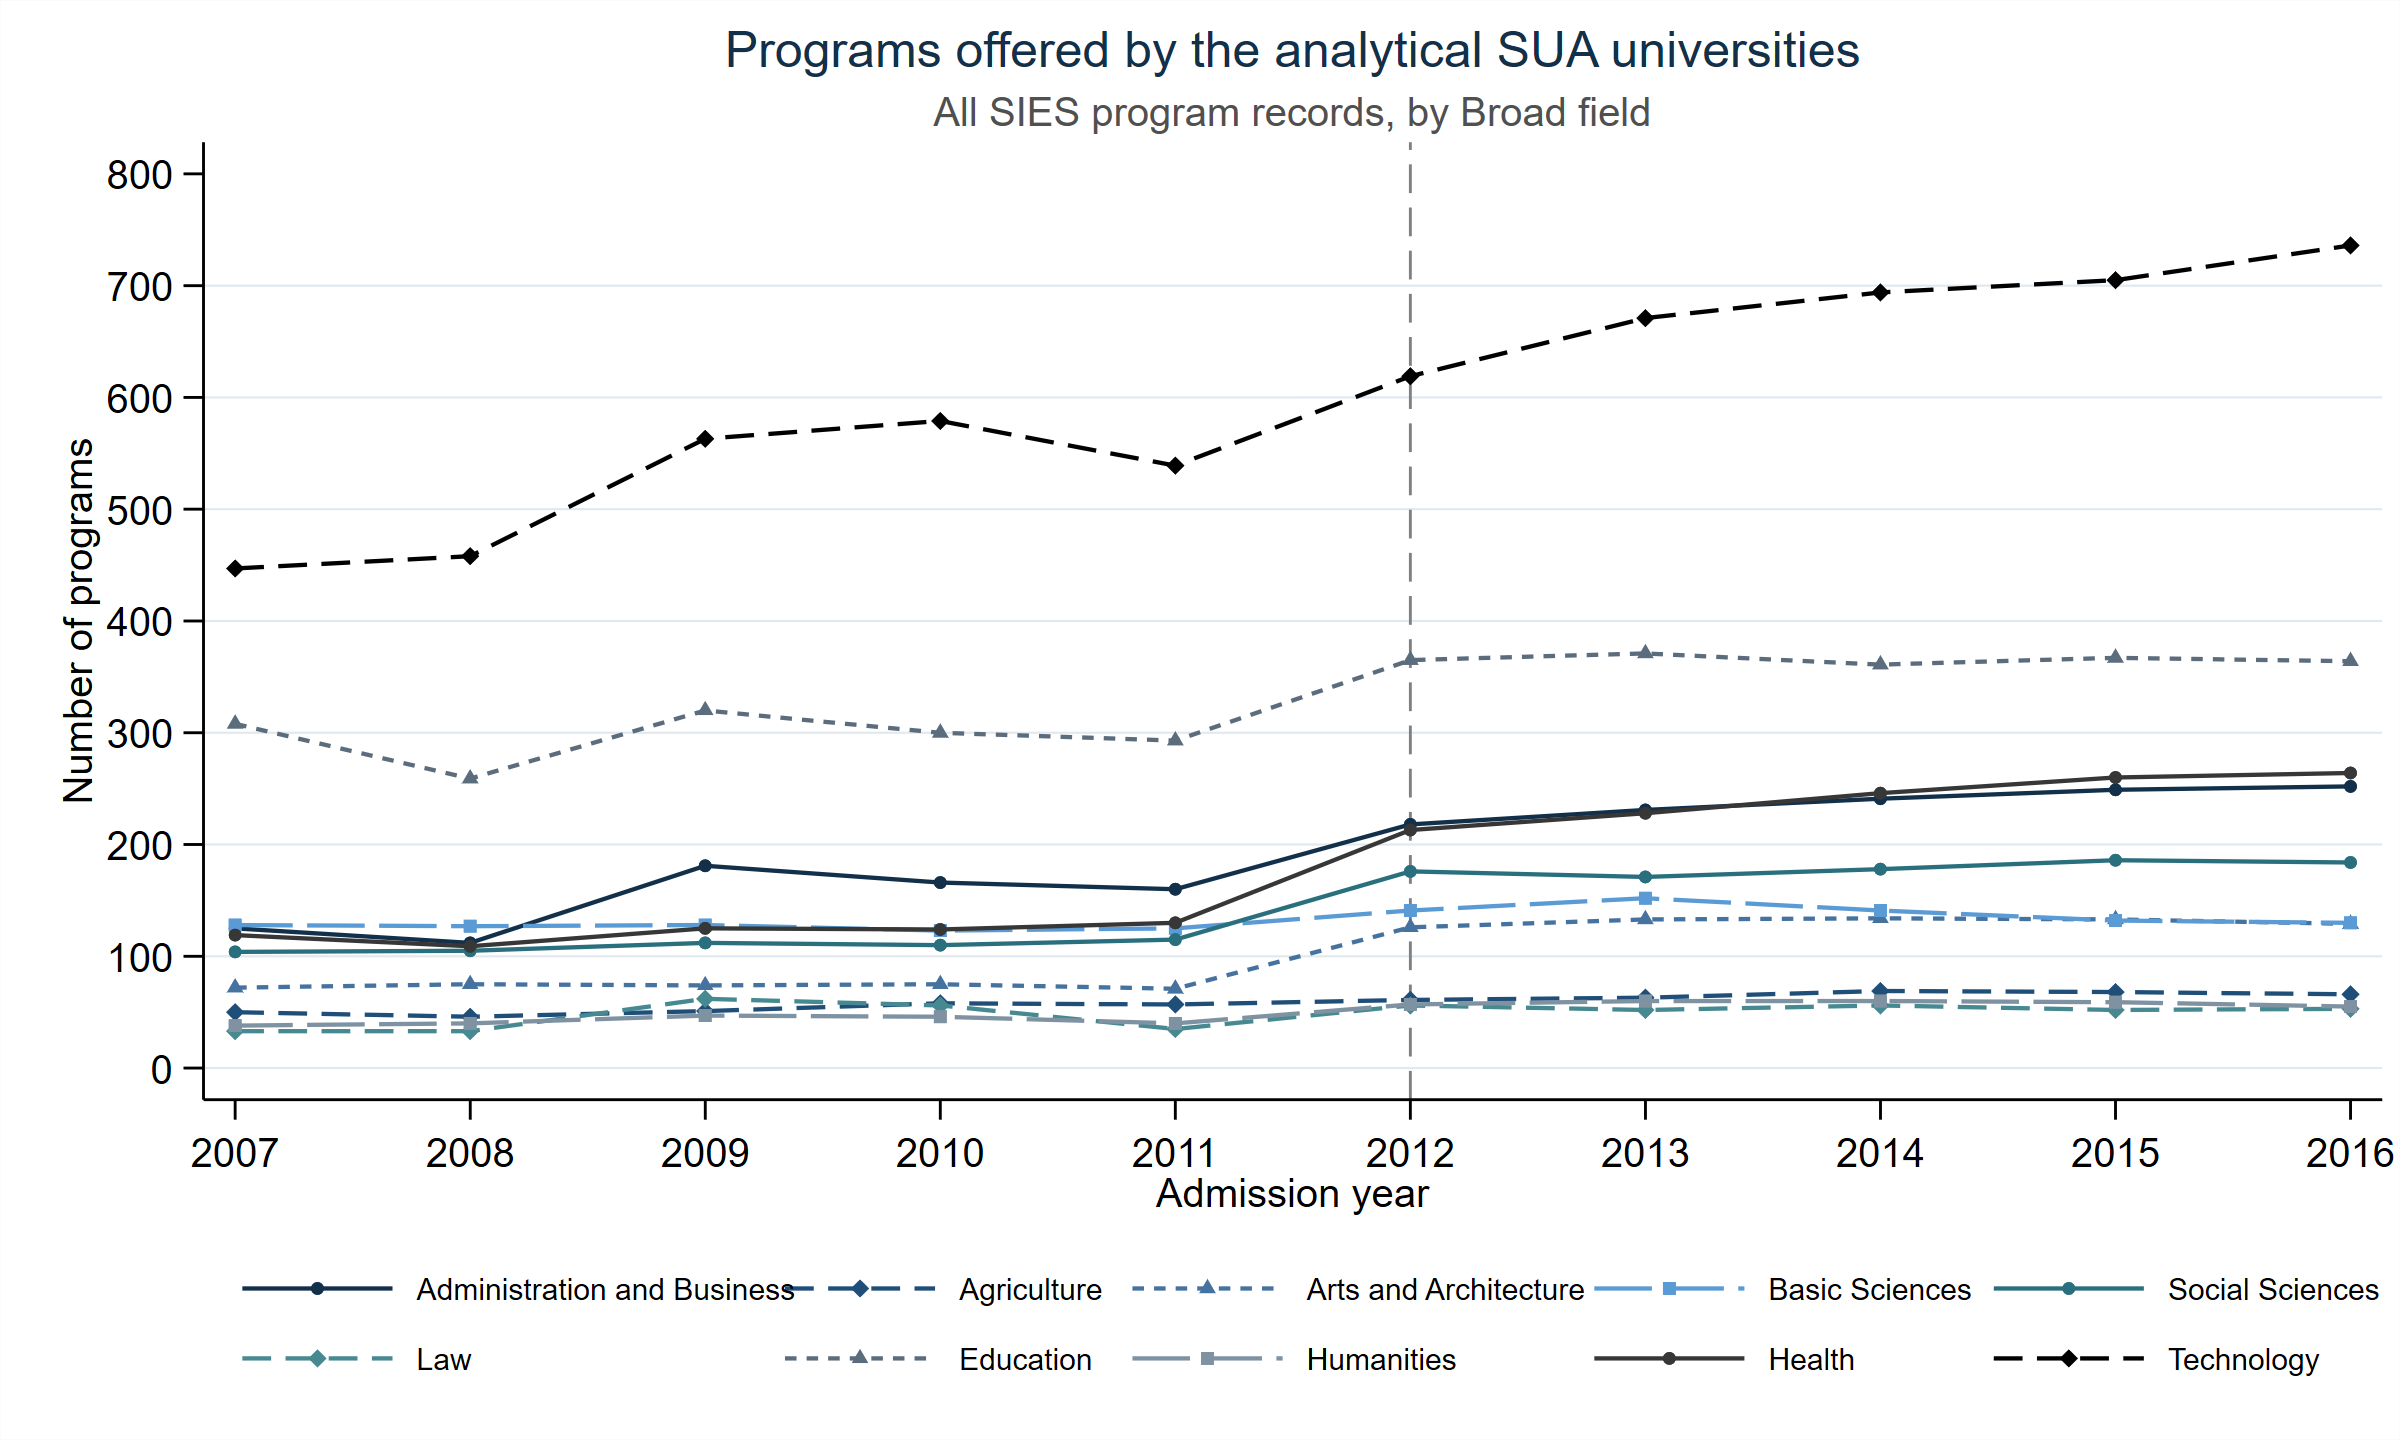
\includegraphics[ width=\linewidth ]{../../output/sua_programs_over_time_by_field.png}

\end{column}

\end{columns}

\vspace{0.08cm}

\begin{itemize}
    \scriptsize
    \setlength{\itemsep}{2pt}

    \item The incorporation of the eight entrant universities adds roughly
    470 programs in 2012. Their program supply remains relatively stable
    afterward, while incumbents account for most subsequent growth.

    \item Technology represents the largest field and an important share of
    program expansion. 
\end{itemize}

\end{frame}

\begin{frame}{Construction of the exposure measures}

\scriptsize
\setlength{\abovedisplayskip}{3pt}
\setlength{\belowdisplayskip}{3pt}

%------------------------------------------------
\begin{columns}[T,onlytextwidth]

\begin{column}{0.49\textwidth}
\textbf{1. Pre-reform enrollment in market $m$}

\begin{center}
\resizebox{0.92\linewidth}{!}{
$\displaystyle
A_m
=
\sum_{\substack{q\in\mathcal E\\ m(q)=m}}
\overline{N}^{\mathrm{first}}_{q,2009\text{--}2011},
\qquad
T_m
=
\sum_{\substack{q\\ m(q)=m}}
\overline{N}^{\mathrm{first}}_{q,2009\text{--}2011}
$
}
\end{center}

\vspace{-0.1cm}

\begin{itemize}
\tiny
\setlength{\itemsep}{0pt}

\item $\mathcal E$ is the set of entrant programs and $m(q)$ is program
$q$'s pre-treatment region $\times$ field market.

\item $\overline{N}^{\mathrm{first}}_{q,2009\text{--}2011}$ is average
first-year enrollment: $A_m$ is entrant and $T_m$ total enrollment in $m$.

\end{itemize}
\end{column}

\begin{column}{0.49\textwidth}
\textbf{2. Total exposure}

\begin{center}
\resizebox{0.26\linewidth}{!}{
$\displaystyle
E_p
=
\frac{A_{m(p)}}{T_{m(p)}}
$
}
\end{center}

\vspace{-0.1cm}

\begin{itemize}
\tiny
\setlength{\itemsep}{0pt}

\item Entrant share of pre-reform first-year enrollment in the market of
incumbent program $p$.

\item Incumbents in the same region $\times$ field market share the
same $E_p$.

\end{itemize}
\end{column}

\end{columns}

\vspace{0.35cm}

%------------------------------------------------
\begin{columns}[T,onlytextwidth]

\begin{column}{0.49\textwidth}
\textbf{3. Selectivity-weighted exposure}

\begin{center}
\resizebox{0.92\linewidth}{!}{
$\displaystyle
E_p^{k}
=
\frac{
\sum_{\substack{q\in\mathcal E\\ m(q)=m(p)}}
k\!\left(|S_p-S_q|\right)
\overline{N}^{\mathrm{first}}_{q,2009\text{--}2011}
}{
T_{m(p)}
}
$
}
\end{center}

\vspace{-0.1cm}

\begin{itemize}
\tiny
\setlength{\itemsep}{0pt}

\item $S_p$, $S_q$: pre-reform mean PSU scores of incumbent $p$ and
entrant $q$; $|S_p-S_q|$ is their selectivity distance.

\item $k\in\{\mathrm{Triangular},\mathrm{Gaussian}\}$ gives greater weight
to closer entrants, so $E_p^k$ varies within a market.

\end{itemize}
\end{column}

\begin{column}{0.49\textwidth}
\textbf{4. Kernel-weighted denominator}

\begin{center}
\resizebox{0.92\linewidth}{!}{
$\displaystyle
E_p^{k,\mathrm{KD}}
=
\frac{
\sum_{\substack{q\in\mathcal E\\ m(q)=m(p)}}
k\!\left(|S_p-S_q|\right)
\overline{N}^{\mathrm{first}}_{q,2009\text{--}2011}
}{
\sum_{\substack{\ell\\ m(\ell)=m(p)}}
k\!\left(|S_p-S_\ell|\right)
\overline{N}^{\mathrm{first}}_{\ell,2009\text{--}2011}
}
$
}
\end{center}

\vspace{-0.1cm}

\begin{itemize}
\tiny
\setlength{\itemsep}{0pt}

\item Same numerator as in 3; the denominator weights every program $\ell$
in the market (incumbents, including $p$, and entrants) by its
selectivity distance to $p$.

\item $E_p^{k,\mathrm{KD}}\in[0,1]$ is the entrant share of the enrollment
that is close to $p$ in selectivity.

\end{itemize}
\end{column}

\end{columns}

\end{frame}

%---------------------------------------------------------
\begin{frame}{SUA exposure: samples and descriptive statistics}

\begin{table}
\centering
\tiny

\renewcommand{\arraystretch}{0.95}

\textit{Panel A: Analytical samples}

\vspace{0.02cm}

\resizebox{0.70\textwidth}{!}{
\begin{tabular}{lrrr}
\toprule
Variable
    & Broad
    & ISCED-97
    & Generic \\
\midrule

Programs
    & 949
    & 949
    & 945 \\

Program-year observations
    & 8,041
    & 8,030
    & 8,002 \\

Incumbent universities
    & 25
    & 25
    & 25 \\

Pre-treatment markets
    & 130
    & 215
    & 638 \\

Mean annual enrollment, 2009--2011
    & 53.2
    & 53.2
    & 53.2 \\

Mean PSU score, 2009--2011
    & 588.8
    & 588.8
    & 589.0 \\

\bottomrule
\end{tabular}
}

\vspace{0.08cm}

\textbf{Panel B. Exposure by academic-field definition}

\vspace{0.03cm}

\resizebox{0.70\textwidth}{!}{
\begin{tabular}{llrrr}
\toprule
Field definition
    & Exposure measure
    & Mean
    & Std. dev.
    & Share zero \\
\midrule

Broad
    & Total
    & 18.53 & 22.21 & 37.7\% \\

    & Triangular
    & 3.48 & 5.57 & 46.8\% \\

    & Gaussian
    & 8.58 & 11.26 & 37.7\% \\

\addlinespace[0.05cm]

ISCED-97
    & Total
    & 17.88 & 22.96 & 43.0\% \\

    & Triangular
    & 3.16 & 5.79 & 56.9\% \\

    & Gaussian
    & 8.20 & 11.70 & 43.0\% \\

\addlinespace[0.05cm]

Generic
    & Total
    & 13.27 & 23.40 & 66.2\% \\

    & Triangular
    & 1.83 & 6.13 & 83.4\% \\

    & Gaussian
    & 5.83 & 11.90 & 67.4\% \\

\bottomrule
\end{tabular}
}

\vspace{0.06cm}

\parbox{0.94\textwidth}{
\tiny
\textit{Notes:}
Panel A reports the analytical sample under each field definition.
Enrollment is the unweighted mean across programs of average annual
first-year enrollment in 2009--2011; PSU is the program's mean score over
the same period. Panel B reports unweighted exposure moments in percentage
points, including zero-exposure programs. Total is the entrant share of
market enrollment; Triangular and Gaussian additionally weight entrant
enrollment by PSU proximity using a 50-point bandwidth. Markets combine
pre-treatment region with the corresponding field definition.
}

\end{table}

\end{frame}

%---------------------------------------------------------
%---------------------------------------------------------
\begin{frame}[label=sua-exposure-main]

\frametitle{
    Distribution of SUA exposure measures
    \hfill
    \hyperlink{sua-exposure-appendix}{
        \scriptsize\color{blue}Alternative fields $\rightarrow$
    }
}

\centering

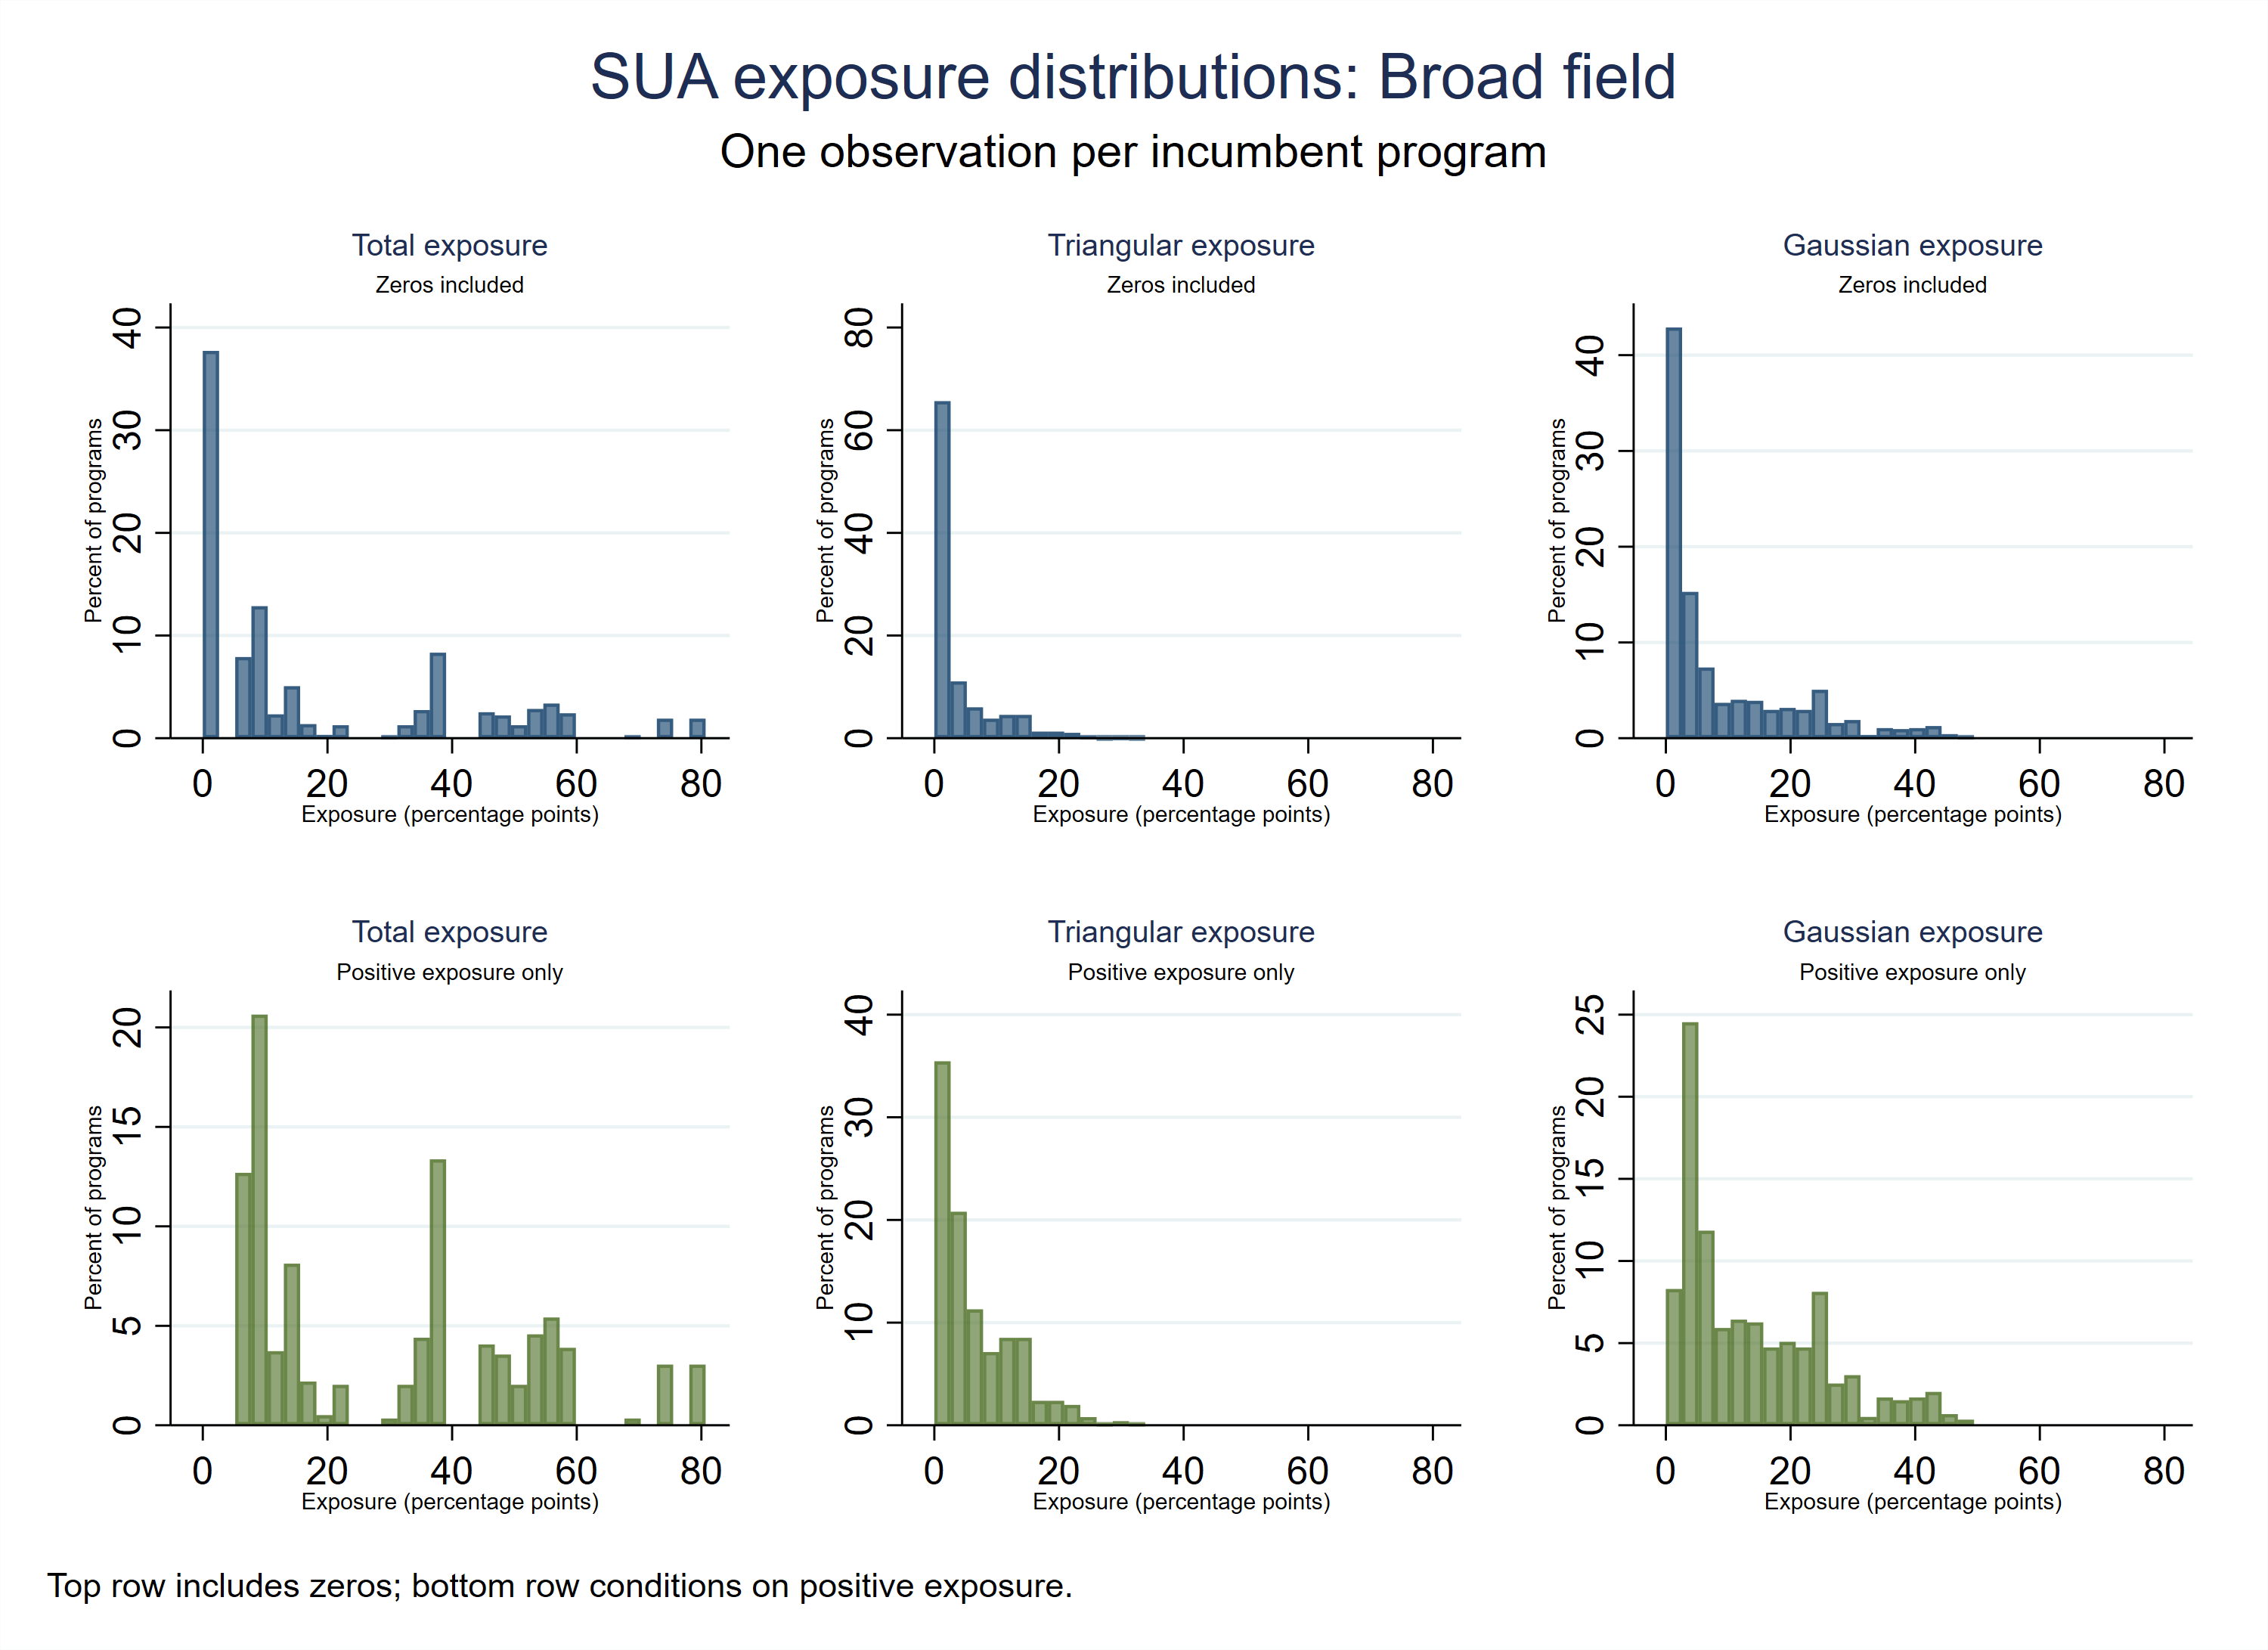
\includegraphics[ width=0.82\textwidth, height=0.64\textheight, keepaspectratio ]{../../output/sua_exposure_distributions_broad.png}

\vspace{-0.10cm}

\begin{itemize}
    \scriptsize
    \setlength{\itemsep}{2pt}

    \item Each incumbent program appears once. The horizontal axis reports
    exposure in percentage points and the vertical axis the share of programs.

    \item The upper row includes all programs; the lower row excludes zeros
    and shows the distribution conditional on positive exposure.

    \item Total exposure has the largest values. Triangular weighting is the
    most restrictive, while Gaussian weighting produces an intermediate
    distribution.
\end{itemize}

\end{frame}


%------------------------------------------------

\begin{frame}{First-stage specification}

\footnotesize

\[
N^{\mathrm{first}}_{pt}
=
\pi_k\left(E_p^k\times Post_t\right)
+\mu_p+\alpha_{f(p),t}
+\gamma_{r(p),t}+\nu_{pt}.
\]

\begin{itemize}
\setlength{\itemsep}{3pt}

\item $p$ indexes incumbent programs and $t$ years.
$N^{\mathrm{first}}_{pt}$ is first-year enrollment of program $p$ in year $t$,
while $E_p^k$ is its pre-reform exposure and $Post_t=1$ in 2012--2016.

\item $f(p)$ denotes the pre-treatment field of program $p$ and $r(p)$ its
pre-treatment region. Accordingly, $\alpha_{f(p),t}$ are field $\times$ year
fixed effects and $\gamma_{r(p),t}$ are region $\times$ year fixed effects.

\item $\mu_p$ denotes program fixed effects, and $\pi_k$ is the post-2012
enrollment difference associated with a 10 percentage-point increase in
exposure measure $k$.

\end{itemize}

\vspace{0.08cm}
\textbf{Exposure is positive in only four regions}

\begin{itemize}
\setlength{\itemsep}{3pt}

\item In the 2009--2011 analytical sample, entrant universities offered
regular undergraduate programs only in Metropolitana, Valparaíso,
Biobío and La Araucanía.

\item Thus, these are the only regions containing entrant programs and
positive entrant enrollment before integration into the SUA.

\item In every other region, the entrant-enrollment numerator is zero:
$A_m=0$, and therefore $E_p=A_{m(p)}/T_{m(p)}=0$.

\end{itemize}

\end{frame}

%---------------------------------------------------------
\begin{frame}[label=sua-first-stage]

\frametitle{
    First stage: exposure to entrant universities
    \hfill
    \hyperlink{sua-event-studies}{
        \scriptsize\color{blue}
        Event studies $\rightarrow$
    }
}

\centering

\begin{equation*}
N^{\mathrm{first}}_{pt}
=
\pi
\left(
E^{k,m}_{p}\times Post_t
\right)
+\mu_p
+\alpha_{f_m(p),t}
+\gamma_{r(p),t}
+\nu_{pt}.
\end{equation*}

\vspace{-0.15cm}

\scriptsize

\resizebox{0.7\textwidth}{!}{%
\begin{tabular}{lcccccc}
\toprule
&
\multicolumn{3}{c}{Field $\times$ year FE}
&
\multicolumn{3}{c}{$+$ Region $\times$ year FE}
\\
\cmidrule(lr){2-4}
\cmidrule(lr){5-7}

Exposure measure
&
Broad
&
ISCED-97
&
Generic
&
Broad
&
ISCED-97
&
Generic
\\
\midrule

\textit{Total}
    & 1.967$^{***}$
    & 1.893$^{***}$
    & 1.872$^{***}$
    & 0.798
    & 0.904$^{*}$
    & 0.324
\\

    & (0.336)
    & (0.335)
    & (0.289)
    & (0.662)
    & (0.510)
    & (0.338)
\\

\quad Wald $F$
    & 34.36
    & 31.92
    & 41.90
    & 1.45
    & 3.14
    & 0.92
\\

\addlinespace[0.08cm]

\textit{Triangular}
    & 0.935
    & 1.392
    & 2.185$^{**}$
    & $-$5.252$^{**}$
    & $-$3.415$^{***}$
    & $-$0.975
\\

    & (0.972)
    & (0.934)
    & (0.927)
    & (2.115)
    & (1.310)
    & (0.829)
\\

\quad Wald $F$
    & 0.93
    & 2.22
    & 5.56
    & 6.17
    & 6.80
    & 1.39
\\

\addlinespace[0.08cm]

\textit{Gaussian}
    & 1.775$^{***}$
    & 1.939$^{***}$
    & 2.342$^{***}$
    & $-$2.767$^{*}$
    & $-$1.447$^{*}$
    & $-$0.558
\\

    & (0.439)
    & (0.450)
    & (0.533)
    & (1.401)
    & (0.832)
    & (0.571)
\\

\quad Wald $F$
    & 16.36
    & 18.60
    & 19.33
    & 3.90
    & 3.03
    & 0.96
\\

\midrule

Observations
    & 8,041
    & 8,030
    & 7,756
    & 8,038
    & 8,027
    & 7,753
\\

Programs
    & 949
    & 949
    & 922
    & 948
    & 948
    & 921
\\

Markets
    & 130
    & 215
    & 615
    & 129
    & 214
    & 614
\\

Program FE
    & Yes & Yes & Yes
    & Yes & Yes & Yes
\\

Field $\times$ year FE
    & Yes & Yes & Yes
    & Yes & Yes & Yes
\\

Region $\times$ year FE
    & No & No & No
    & Yes & Yes & Yes
\\

\bottomrule
\end{tabular}%
}

\vspace{0.08cm}

\parbox{0.97\textwidth}{%
\tiny
\textit{Notes:}
The dependent variable is first-year enrollment in incumbent CRUCH programs.
Total exposure is entrants' pre-treatment enrollment share; Triangular and
Gaussian additionally weight entrant enrollment by PSU-score proximity using
a 50-point bandwidth. Markets combine pre-treatment region with the indicated
field definition. Exposure is interacted with $Post_t$, equal to one in
2012--2016, and measured in 10 percentage-point units. All regressions absorb
program and corresponding field $\times$ year fixed effects; the last three
columns additionally absorb region $\times$ year fixed effects. Standard
errors are clustered by the corresponding pre-treatment market and reported
in parentheses. Wald $F$ statistics test the exposure coefficient. Sample
differences reflect singleton removal by \texttt{reghdfe}.
$^{***}p<0.01$, $^{**}p<0.05$, $^{*}p<0.10$.
Robustness: \hyperlink{sua-fs-lvl-entrant}{\color{blue}regions with entrant
universities only $\rightarrow$} \quad
\hyperlink{sua-fs-lvl-positive}{\color{blue}positive exposure only $\rightarrow$}
}

\end{frame}


%---------------------------------------------------------
\begin{frame}[label=sua-log-first-stage]

\frametitle{
SUA exposure: log-log first stages
\hfill
\hyperlink{sua-log-event-studies}{
\scriptsize\color{blue}
Event studies $\rightarrow$
}
}

\centering
\scriptsize

%---------------------------------------------------------
% SPECIFICATION
%---------------------------------------------------------

\begin{center}
\resizebox{0.87\textwidth}{!}{
$
\begin{gathered}
\log N^{\mathrm{first}}_{pt}
=
\beta_k
\left[
\widetilde{\log E_p^k}\times Post_t
\right]
+
\theta_k
\left[
D_p^k\times Post_t
\right]
+
\mu_p+\alpha_{f(p),t}
+\gamma_{r(p),t}
+\varepsilon_{pt},
\\[0.12cm]
\widetilde{\log E_p^k}
=
\begin{cases}
\log(E_p^k), & E_p^k>0,\\
0, & E_p^k=0,
\end{cases}
\qquad
D_p^k=\mathbf{1}\{E_p^k>0\}.
\end{gathered}
$
}
\end{center}

\vspace{0.06cm}

%---------------------------------------------------------
% RESULTS
%---------------------------------------------------------

\resizebox{0.95\textwidth}{!}{
\begin{tabular}{lcccccc}
\toprule
&
\multicolumn{3}{c}{Field $\times$ year FE}
&
\multicolumn{3}{c}{$+$ Region $\times$ year FE}
\\
\cmidrule(lr){2-4}
\cmidrule(lr){5-7}

Exposure measure
& Broad
& ISCED-97
& Generic
& Broad
& ISCED-97
& Generic
\\
\midrule

\textit{Total}
& 0.100$^{***}$ (0.034)
& 0.072$^{**}$ (0.035)
& 0.021 (0.030)
& $-$0.005 (0.039)
& $-$0.024 (0.032)
& $-$0.022 (0.027)
\\

\quad $F$
& 8.84 & 4.24 & 0.48
& 0.01 & 0.55 & 0.69
\\

\addlinespace[0.07cm]

\textit{Triangular}
& $-$0.013 (0.015)
& 0.004 (0.016)
& 0.016 (0.021)
& $-$0.050$^{***}$ (0.017)
& $-$0.024 (0.016)
& $-$0.005 (0.017)
\\

\quad $F$
& 0.81 & 0.07 & 0.59
& 8.95 & 2.37 & 0.07
\\

\addlinespace[0.07cm]

\textit{Gaussian}
& $-$0.026 (0.032)
& $-$0.024 (0.030)
& 0.001 (0.018)
& $-$0.107$^{***}$ (0.030)
& $-$0.079$^{***}$ (0.026)
& $-$0.025 (0.017)
\\

\quad $F$
& 0.68 & 0.64 & 0.01
& 12.72 & 9.35 & 2.19
\\

\midrule

Observations
& 8,041 & 8,030 & 7,756
& 8,038 & 8,027 & 7,753
\\

Programs
& 949 & 949 & 922
& 948 & 948 & 921
\\

\bottomrule
\end{tabular}
}

\vspace{0.10cm}

%---------------------------------------------------------
% NOTES
%---------------------------------------------------------

\parbox{0.94\textwidth}{
\tiny
\textit{Notes:}
Each coefficient reports $\beta_k$, the post-2012 elasticity with respect
to exposure intensity. Zero-exposure programs are retained by setting
$\widetilde{\log E_p^k}=0$ when $E_p^k=0$ and including
$D_p^k\times Post_t$ separately; the coefficient on this indicator is not
reported. Thus, $\beta_k$ captures variation in exposure intensity among
positively exposed programs while allowing zero-exposure programs to remain
in the estimation sample. All specifications absorb program and corresponding
field $\times$ year fixed effects; the last three columns additionally absorb
pre-treatment region $\times$ year fixed effects. Standard errors are clustered
at the pre-treatment market level. Observations with zero first-year enrollment
are excluded because the dependent variable is in logs.
$^{*}p<0.10$, $^{**}p<0.05$, $^{***}p<0.01$.
Robustness: \hyperlink{sua-fs-log-entrant}{\color{blue}regions with entrant
universities only $\rightarrow$} \quad
\hyperlink{sua-fs-log-positive}{\color{blue}positive exposure only $\rightarrow$}
}

\end{frame}

%---------------------------------------------------------
\begin{frame}[label=sua-kd-first-stage]

\frametitle{
    First stage: kernel-weighted denominator
    \hfill
    \hyperlink{sua-kd-event-studies}{\scriptsize\color{blue}Event studies $\rightarrow$}
}

\centering

{\small
\begin{equation*}
N^{\mathrm{first}}_{pt}
=
\pi
\left(
E^{k,\mathrm{KD}}_{p}\times Post_t
\right)
+\mu_p
+\alpha_{f_m(p),t}
+\gamma_{r(p),t}
+\nu_{pt}.
\end{equation*}
}

\vspace{-0.2cm}

\resizebox{0.66\textwidth}{!}{\begin{tabular}{lcccccc}
\toprule
 & \multicolumn{3}{c}{Field \(\times\) year FE} & \multicolumn{3}{c}{\(+\) Region \(\times\) year FE} \\
\cmidrule(lr){2-4}\cmidrule(lr){5-7}
Exposure measure & Broad & ISCED-97 & Generic & Broad & ISCED-97 & Generic \\
\midrule
\textit{Triangular KD} &  0.659\sym{**} &  0.717\sym{**} &  1.371\sym{***} & -1.726\sym{**} & -1.286\sym{***} & -0.208 \\
 & (0.299) & (0.292) & (0.481) & (0.737) & (0.427) & (0.470) \\
\quad Wald \(F\) &  4.86 &  6.03 &  8.13 &  5.48 &  9.08 &  0.20 \\
\quad Programs with zero exposure &       444 &       540 &       767 &       443 &       539 &       766 \\
\addlinespace
\textit{Gaussian KD} &  1.326\sym{***} &  1.420\sym{***} &  1.913\sym{***} & -1.919\sym{*} & -1.049\sym{*} & -0.218 \\
 & (0.346) & (0.350) & (0.394) & (1.051) & (0.600) & (0.472) \\
\quad Wald \(F\) & 14.70 & 16.42 & 23.56 &  3.33 &  3.06 &  0.21 \\
\quad Programs with zero exposure &       358 &       408 &       616 &       357 &       407 &       615 \\
\midrule
Observations &     8,041 &     8,030 &     7,756 &     8,038 &     8,027 &     7,753 \\
Programs &       949 &       949 &       922 &       948 &       948 &       921 \\
Markets &       130 &       215 &       615 &       129 &       214 &       614 \\
Program FE & Yes & Yes & Yes & Yes & Yes & Yes \\
Field \(\times\) year FE & Yes & Yes & Yes & Yes & Yes & Yes \\
Region \(\times\) year FE & No & No & No & Yes & Yes & Yes \\
\bottomrule
\end{tabular}
}

\vspace{0.08cm}

\parbox{0.97\textwidth}{%
\tiny
\textit{Notes:}
Exposure uses the kernel-weighted denominator (point 4 of the exposure construction): the denominator weights every program in the market by its selectivity distance to $p$, with the same 50-point Triangular and Gaussian kernels as the numerator. Sample and fixed effects as in the main first stage; SE clustered by pre-treatment market.
Exposure in 10 percentage-point units. As in the
\hyperlink{sua-first-stage}{\color{blue}main first stage}, coefficients are
positive with field $\times$ year FE and negative with region $\times$ year FE.
Magnitudes are smaller because KD exposure takes larger values (Broad, 2011
mean: 0.11 for Triangular KD vs.\ 0.03 for Triangular).
$^{***}p<0.01$, $^{**}p<0.05$, $^{*}p<0.10$.
}

\end{frame}

%---------------------------------------------------------
\begin{frame}[label=sua-kd-log-first-stage]

\frametitle{
    Log first stage: kernel-weighted denominator
    \hfill
    \hyperlink{sua-kd-log-event-studies}{\scriptsize\color{blue}Event studies $\rightarrow$}
}

\centering

\vspace{0.2cm}

\resizebox{0.85\textwidth}{!}{%
$\log N^{\mathrm{first}}_{pt}
=
\beta_k\left[\widetilde{\log E_p^{k,\mathrm{KD}}}\times Post_t\right]
+\theta_k\left[D_p^k\times Post_t\right]
+\mu_p+\alpha_{f(p),t}+\gamma_{r(p),t}+\varepsilon_{pt}.$}

\vspace{0.3cm}

\vspace{-0.2cm}

\resizebox{0.66\textwidth}{!}{\begin{tabular}{lcccccc}
\toprule
 & \multicolumn{3}{c}{Field \(\times\) year FE} & \multicolumn{3}{c}{\(+\) Region \(\times\) year FE} \\
\cmidrule(lr){2-4}\cmidrule(lr){5-7}
Exposure measure & Broad & ISCED-97 & Generic & Broad & ISCED-97 & Generic \\
\midrule
\textit{Triangular KD} & -0.001 &  0.014 &  0.022 & -0.052\sym{***} & -0.032\sym{*} & -0.014 \\
 & (0.014) & (0.018) & (0.023) & (0.018) & (0.017) & (0.018) \\
\quad Wald \(F\) &  0.00 &  0.60 &  0.96 &  8.86 &  3.83 &  0.60 \\
\quad Programs with zero exposure &       444 &       540 &       767 &       443 &       539 &       766 \\
\addlinespace
\textit{Gaussian KD} & -0.012 & -0.018 &  0.009 & -0.138\sym{***} & -0.095\sym{***} & -0.030\sym{*} \\
 & (0.036) & (0.032) & (0.019) & (0.037) & (0.028) & (0.018) \\
\quad Wald \(F\) &  0.12 &  0.32 &  0.24 & 13.59 & 11.31 &  3.01 \\
\quad Programs with zero exposure &       358 &       408 &       616 &       357 &       407 &       615 \\
\midrule
Observations &     8,041 &     8,030 &     7,756 &     8,038 &     8,027 &     7,753 \\
Programs &       949 &       949 &       922 &       948 &       948 &       921 \\
Markets &       130 &       215 &       615 &       129 &       214 &       614 \\
Program FE & Yes & Yes & Yes & Yes & Yes & Yes \\
Field \(\times\) year FE & Yes & Yes & Yes & Yes & Yes & Yes \\
Region \(\times\) year FE & No & No & No & Yes & Yes & Yes \\
\bottomrule
\end{tabular}
}

\vspace{0.08cm}

\parbox{0.97\textwidth}{%
\tiny
\textit{Notes:}
Exposure uses the kernel-weighted denominator (point 4 of the exposure construction): the denominator weights every program in the market by its selectivity distance to $p$, with the same 50-point Triangular and Gaussian kernels as the numerator. Sample and fixed effects as in the main first stage; SE clustered by pre-treatment market.
$\widetilde{\log E}=\log E$ if $E>0$ and 0 otherwise; $D_p^k=\mathbf{1}\{E_p^{k,\mathrm{KD}}>0\}$.
Observations with zero first-year enrollment are excluded. Compare with the
\hyperlink{sua-log-first-stage}{\color{blue}main log first stage}.
$^{***}p<0.01$, $^{**}p<0.05$, $^{*}p<0.10$.
}

\end{frame}
%---------------------------------------------------------


%---------------------------------------------------------
%---------------------------------------------------------



%---------------------------------------------------------



%---------------------------------------------------------
\begin{frame}[label=sua-selectivity-heterogeneity]

\frametitle{First-stage heterogeneity by incumbent selectivity}

\centering

\begin{table}
\centering
\tiny
\setlength{\tabcolsep}{4.5pt}
\renewcommand{\arraystretch}{0.95}

\begin{tabular}{lcccccc}
\toprule
& \multicolumn{2}{c}{PSU $<550$}
& \multicolumn{2}{c}{PSU $550$--$649$}
& \multicolumn{2}{c}{PSU $\geq650$} \\
\cmidrule(lr){2-3}
\cmidrule(lr){4-5}
\cmidrule(lr){6-7}
& Tri.
& Gau.
& Tri.
& Gau.
& Tri.
& Gau. \\
\midrule

\multicolumn{7}{l}{\textit{SUA exposure}} \\[2pt]

Coefficient
& $-1.61$
& $-0.54$
& $-3.17^{**}$
& $-0.98$
& $-15.75^{*}$
& $-5.01$ \\

& $(2.78)$
& $(2.10)$
& $(1.54)$
& $(0.83)$
& $(8.25)$
& $(4.38)$ \\

$F$-statistic
& 0.34
& 0.07
& 4.26
& 1.41
& 3.65
& 1.31 \\


Observations
& \multicolumn{2}{c}{2,215}
& \multicolumn{2}{c}{4,609}
& \multicolumn{2}{c}{1,188} \\

Programs
& \multicolumn{2}{c}{272}
& \multicolumn{2}{c}{531}
& \multicolumn{2}{c}{143} \\

Clusters
& \multicolumn{2}{c}{89}
& \multicolumn{2}{c}{100}
& \multicolumn{2}{c}{25} \\

\bottomrule
\end{tabular}
\end{table}

\vspace{-0.05cm}


\parbox{0.95\textwidth}{
\tiny
\textit{Notes:}
Standard errors clustered by pre-treatment market in parentheses.
All regressions include program, Broad-field$\times$year, and region$\times$year FE.
Coefficients correspond to a 10 percentage-point increase in exposure.
The same split for conditional similarity is in the
\hyperlink{sua-q-heterogeneity}{\color{blue}appendix}.
$^{*}p<0.10$, $^{**}p<0.05$, $^{***}p<0.01$.
}

\end{frame}

% COSINE EXPOSURE
%=========================================================

%---------------------------------------------------------
\begin{frame}{Cosine exposure}

\scriptsize
\setlength{\abovedisplayskip}{2pt}
\setlength{\belowdisplayskip}{2pt}

\tiny
Each program is represented by a vector describing the distribution of its
2011 first-year students. Each coordinate counts students with a particular
PSU profile and, depending on the definition, campus region and Broad field.
Programs are more similar when their students are distributed across the same
vector cells.

\vspace{0.06cm}

\textbf{1. Program vectors}

\begin{center}
\resizebox{0.82\textwidth}{!}{
\(
\displaystyle
\mathbf v_p^{PSU}
=
(v_{p,b})_{b\in\mathcal B},
\qquad
\mathbf v_p^{PSU\times R}
=
(v_{p,rb})_{\substack{r\in\mathcal R\\b\in\mathcal B}},
\qquad
\mathbf v_p^{PSU\times R\times F}
=
(v_{p,rfb})_{\substack{r\in\mathcal R,\;f\in\mathcal F\\b\in\mathcal B}}.
\)
}
\end{center}

\vspace{-0.10cm}

Here, \(b\) denotes a 25-point PSU bin, \(r\) campus region, and \(f\) Broad
field. Each vector cell contains the number of first-year students in that
combination. Entrant-program vectors are constructed analogously.

\vspace{0.05cm}

\textbf{2. Similarity between incumbent \(p\) and entrant \(j\)}

\begin{center}
\resizebox{0.56\textwidth}{!}{
\(
\displaystyle
\cos\theta^{d}_{j,p}
=
\frac{
\mathbf v_j^{d}\cdot\mathbf v_p^{d}
}{
\lVert\mathbf v_j^{d}\rVert
\lVert\mathbf v_p^{d}\rVert
},
\qquad
d\in
\left\{
PSU,\,
PSU\times R,\,
PSU\times R\times F
\right\}.
\)
}
\end{center}

\vspace{-0.10cm}

The cosine compares the \textbf{shape of the student distributions}, rather
than program size. Under interaction-cell definitions, similarity is zero
when programs do not share the indicated region or field.

\vspace{0.05cm}

\textbf{3. Additive similarity measures}

\begin{center}
\resizebox{0.80\textwidth}{!}{
\(
\displaystyle
\cos\theta^{PSU+R}_{j,p}
=
\frac{
\cos\theta^{PSU}_{j,p}
+
\mathbf 1\{r_j=r_p\}
}{2},
\qquad
\cos\theta^{PSU+R+F}_{j,p}
=
\frac{
\cos\theta^{PSU}_{j,p}
+
\mathbf 1\{r_j=r_p\}
+
\mathbf 1\{f_j=f_p\}
}{3}.
\)
}
\end{center}

\vspace{-0.10cm}

These measures give equal weight to PSU-profile similarity and coincidence
in campus region and, where applicable, Broad field.

\vspace{0.05cm}

\textbf{4. Exposure of incumbent program \(p\)}

\begin{center}
\resizebox{0.42\textwidth}{!}{
\(
\displaystyle
E_p^{d}
=
\sum_{j\in\mathcal J}
w_j\cos\theta^{d}_{j,p},
\qquad
w_j
=
\frac{
N^{\mathrm{first}}_{j,2011}
}{
\sum_{\ell\in\mathcal J}
N^{\mathrm{first}}_{\ell,2011}
}.
\)
}
\end{center}

\vspace{-0.10cm}

Exposure is higher when incumbent \(p\) resembles entrant programs that
account for a larger share of entrant enrollment.

\vspace{0.03cm}

\tiny
\textit{Notes:}
\(\mathcal J\) contains programs from the eight entrant universities.
Campus region is the university program's location in 2011. Student school
region and SES are not used.

\end{frame}
   
%---------------------------------------------------------
\begin{frame}{Cosine exposure: samples and descriptive statistics}

\begin{table}
\centering
\tiny

\renewcommand{\arraystretch}{0.95}

\textit{Panel A: Analytical samples}

\vspace{0.02cm}

\resizebox{0.62\textwidth}{!}{
\begin{tabular}{lrr}
\toprule
Variable
    & Full sample
    & $N^{\mathrm{first}}_{p,2011}\geq10$ \\
\midrule

Programs
    & 996 & 939 \\

Program-year observations
    & 9,105 & 8,618 \\

Incumbent universities
    & 25 & 25 \\

Total first-year enrollment, 2011
    & 54,659 & 54,303 \\

Mean enrollment per program, 2011
    & 54.9 & 57.8 \\

Mean annual enrollment, 2007--2011
    & 54.8 & 57.3 \\

Mean PSU score, 2011
    & 578.0 & 580.9 \\

\bottomrule
\end{tabular}
}

\vspace{0.08cm}

\textit{Panel B: Distribution of raw cosine exposure}

\vspace{0.02cm}

\resizebox{0.95\textwidth}{!}{
\begin{tabular}{lrrrrrr}
\toprule
&
\multicolumn{3}{c}{Full sample}
&
\multicolumn{3}{c}{$N^{\mathrm{first}}_{p,2011}\geq10$}
\\
\cmidrule(lr){2-4}
\cmidrule(lr){5-7}

Exposure measure
    & Mean
    & Std. dev.
    & Share zero
    & Mean
    & Std. dev.
    & Share zero
\\
\midrule

PSU bins
    & 0.4762
    & 0.1559
    & 0.0\%
    & 0.4842
    & 0.1540
    & 0.0\%
\\

PSU bins $\times$ campus region
    & 0.0977
    & 0.1495
    & 37.0\%
    & 0.1024
    & 0.1521
    & 34.7\%
\\

PSU bins $+$ campus region
    & 0.3405
    & 0.1614
    & 0.0\%
    & 0.3490
    & 0.1604
    & 0.0\%
\\

\addlinespace[0.04cm]

PSU bins $\times$ campus region $\times$ Broad field
    & 0.0113
    & 0.0196
    & 38.3\%
    & 0.0119
    & 0.0200
    & 35.8\%
\\

PSU bins $+$ campus region $+$ Broad field
    & 0.2681
    & 0.1078
    & 0.0\%
    & 0.2745
    & 0.1064
    & 0.0\%
\\

\bottomrule
\end{tabular}
}

\vspace{0.06cm}

\parbox{0.95\textwidth}{
\tiny
\textit{Notes:}
The unit is an incumbent SUA program and exposure moments are unweighted
across programs. The restricted sample excludes 57 programs with fewer than
10 first-year students in 2011. Multiplicative measures require coincidence
in the indicated dimensions; additive measures assign equal weight to PSU
similarity, campus-region coincidence and, where applicable, Broad-field
coincidence. The restriction is applied after exposure construction, so
entrant profiles, weights, and exposure scaling remain unchanged. Campus
region is the university program's location; student school region and SES
are not used.
}

\end{table}

\end{frame}

%---------------------------------------------------------

%---------------------------------------------------------
% COSINE EXPOSURE DISTRIBUTIONS
%---------------------------------------------------------
\begin{frame}[label=cosine-exposure-main]

\frametitle{
Distribution of cosine exposure measures
\hfill
\hyperlink{cosine-exposure-positive}{
\scriptsize\color{blue}Positive exposure only $\rightarrow$
}
}

\centering

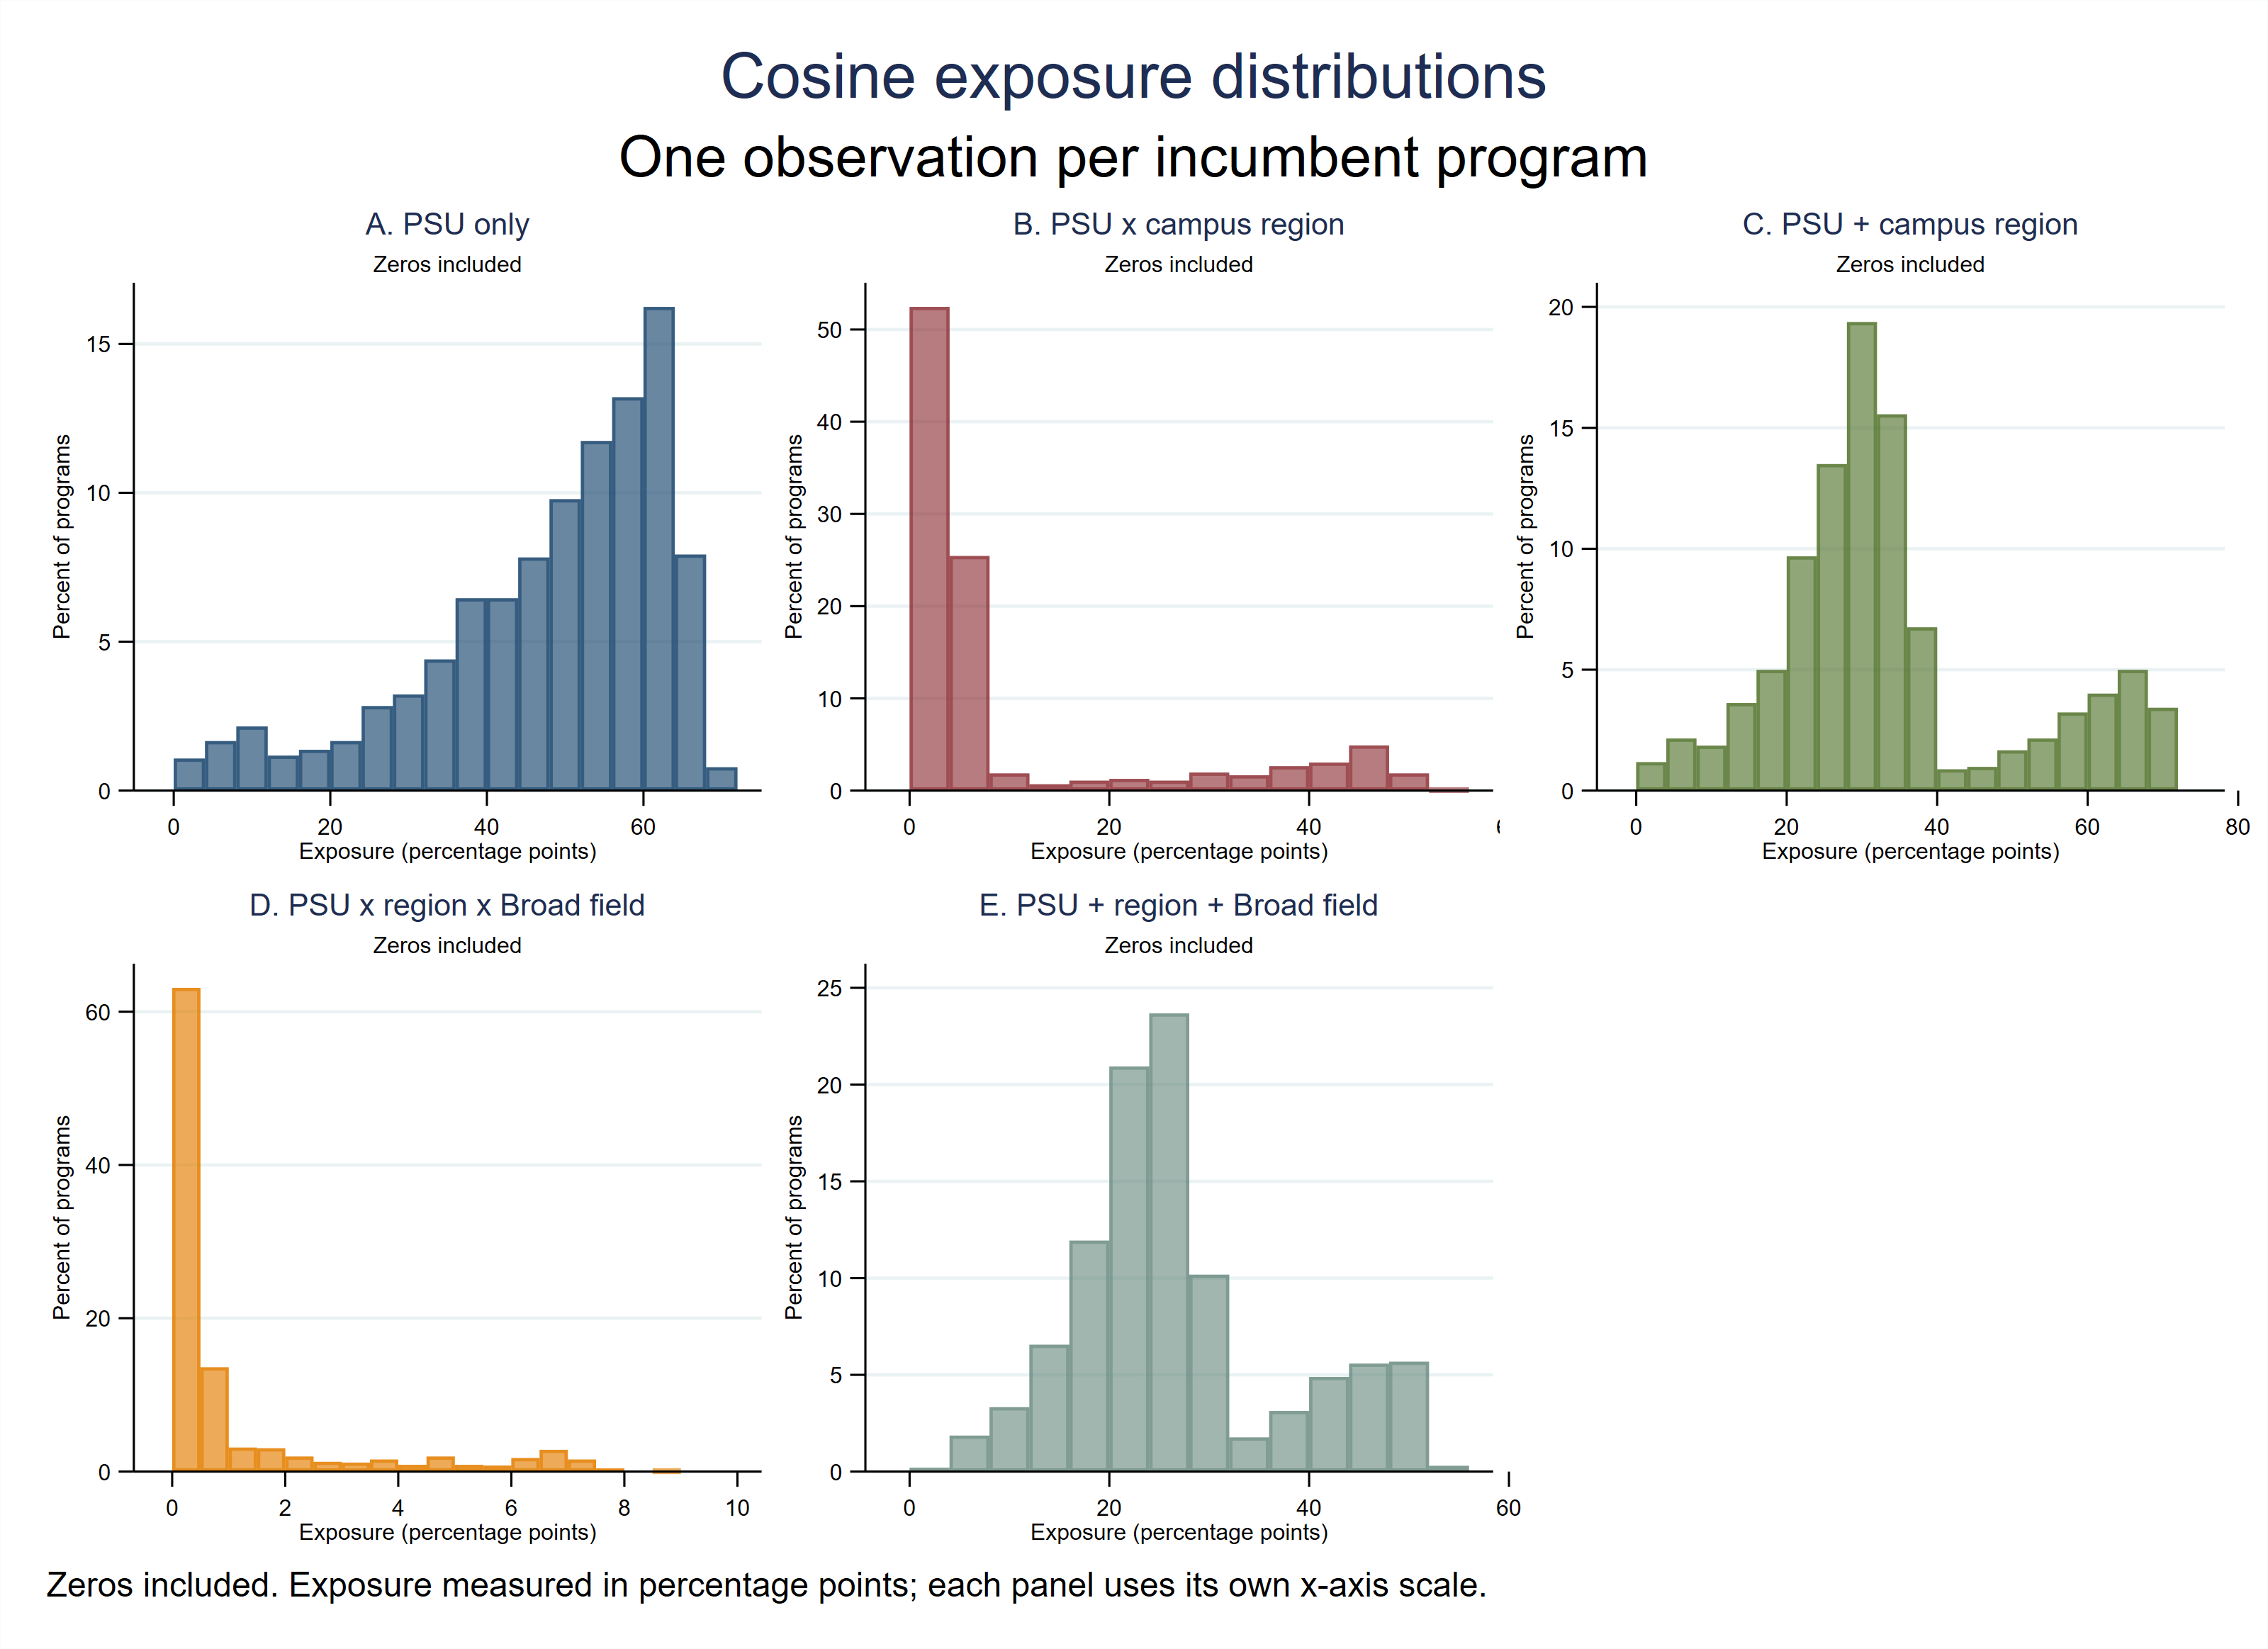
\includegraphics[ width=0.84\textwidth, height=0.64\textheight, keepaspectratio ]{../../output/cosine_exposure_distributions_zero_included.png}

\vspace{-0.10cm}

\tiny
\begin{itemize}
\scriptsize
\setlength{\itemsep}{2pt}

\item Each incumbent program appears once. The horizontal axis reports
cosine exposure in percentage points and the vertical axis the share of
programs.



\item Multiplicative definitions are more restrictive. In particular,
PSU $\times$ campus region $\times$ Broad field places substantial mass at
zero and has a much smaller support than the PSU-only and additive measures.

\end{itemize}

\end{frame}

%---------------------------------------------------------
\begin{frame}
\hypertarget{cosine-first-stage}{}
\frametitle{
    Cosine exposure: first-stage results
    \hfill
    \hyperlink{cosine-event-studies}{
        \scriptsize\color{blue}
        Event studies $\rightarrow$
    }
}

\begin{center}
\resizebox{0.56\textwidth}{!}{
$
\displaystyle
N^{\mathrm{first}}_{pt}
=
\beta_k(E_p^k\times Post_t)
+\mu_p+\alpha_{f(p),t}
+\gamma_{r(p),t}+\varepsilon_{pt}.
$
}
\end{center}

\vspace{-0.14cm}

\begin{table}
\centering
\tiny

\setlength{\tabcolsep}{3.3pt}
\renewcommand{\arraystretch}{0.92}

\resizebox{0.8\textwidth}{!}{
\begin{tabular}{lcccccc}
\toprule
&
\multicolumn{3}{c}{Full sample}
&
\multicolumn{3}{c}{$N^{\mathrm{first}}_{p,2011}\geq10$}
\\
\cmidrule(lr){2-4}
\cmidrule(lr){5-7}

Exposure measure
&
\shortstack{(1)\\$+$ year}
&
\shortstack{(2)\\$+$ field$\times$year}
&
\shortstack{(3)\\$+$ region$\times$year}
&
\shortstack{(4)\\$+$ year}
&
\shortstack{(5)\\$+$ field$\times$year}
&
\shortstack{(6)\\$+$ region$\times$year}
\\
\midrule

%---------------------------------------------------------
% PSU ONLY
%---------------------------------------------------------



PSU bins
    & $-1.811^{*}$
    & $-1.403$
    & $-0.716$
    & $-2.116^{**}$
    & $-1.597$
    & $-0.630$
\\

    & $(0.948)$
    & $(1.018)$
    & $(1.002)$
    & $(1.017)$
    & $(1.098)$
    & $(1.075)$
\\

\quad Wald $F$
    & $3.65$
    & $1.90$
    & $0.51$
    & $4.33$
    & $2.11$
    & $0.34$
\\

\addlinespace[0.06cm]

%---------------------------------------------------------
% MULTIPLICATIVE MEASURES
%---------------------------------------------------------



PSU bins $\times$ region
    & $3.976^{***}$
    & $4.126^{***}$
    & $-5.174$
    & $3.903^{***}$
    & $4.119^{***}$
    & $-5.267$
\\

    & $(0.601)$
    & $(0.598)$
    & $(3.736)$
    & $(0.611)$
    & $(0.611)$
    & $(3.797)$
\\

\quad Wald $F$
    & $43.82$
    & $47.55$
    & $1.92$
    & $40.82$
    & $45.41$
    & $1.92$
\\[0.03cm]

PSU bins $\times$ region $\times$ field
    & $3.680^{***}$
    & $3.624^{***}$
    & $-3.922^{*}$
    & $3.590^{***}$
    & $3.612^{***}$
    & $-4.023^{*}$
\\

    & $(0.658)$
    & $(0.647)$
    & $(2.075)$
    & $(0.666)$
    & $(0.655)$
    & $(2.140)$
\\

\quad Wald $F$
    & $31.33$
    & $31.36$
    & $3.57$
    & $29.09$
    & $30.44$
    & $3.53$
\\

\addlinespace[0.06cm]

%---------------------------------------------------------
% ADDITIVE MEASURES
%---------------------------------------------------------


PSU bins $+$ region
    & $4.299^{***}$
    & $4.416^{***}$
    & $-1.476$
    & $4.344^{***}$
    & $4.577^{***}$
    & $-1.298$
\\

    & $(0.643)$
    & $(0.641)$
    & $(2.066)$
    & $(0.667)$
    & $(0.668)$
    & $(2.217)$
\\

\quad Wald $F$
    & $44.76$
    & $47.54$
    & $0.51$
    & $42.36$
    & $47.02$
    & $0.34$
\\[0.03cm]

PSU bins $+$ region $+$ field
    & $4.639^{***}$
    & $4.429^{***}$
    & $-1.480$
    & $4.728^{***}$
    & $4.590^{***}$
    & $-1.302$
\\

    & $(0.656)$
    & $(0.642)$
    & $(2.071)$
    & $(0.690)$
    & $(0.669)$
    & $(2.224)$
\\

\quad Wald $F$
    & $50.07$
    & $47.54$
    & $0.51$
    & $46.97$
    & $47.02$
    & $0.34$
\\

\midrule

Observations
    & 9,105 & 9,105 & 9,103
    & 8,618 & 8,618 & 8,610
\\

Programs
    & 996 & 996 & 996
    & 939 & 939 & 938
\\

\bottomrule
\end{tabular}
}

\vspace{0.04cm}

\parbox{0.97\textwidth}{
\tiny
\textit{Notes:}
The dependent variable is incumbent-program first-year enrollment.
Coefficients are reported first, program-clustered standard errors are in
parentheses, and Wald $F$ statistics appear in the corresponding labeled
row. Exposure is measured in SD units and $Post_t=1$ in 2012--2016.
Columns (1) and (4) include program and year FE; Columns (2) and (5) use
Broad-field $\times$ year FE; Columns (3) and (6) add campus-region
$\times$ year FE. Multiplicative measures require coincidence in the
indicated dimensions; additive measures combine them with equal weights.
Columns (4)--(6) exclude programs with fewer than 10 first-year students
in 2011. $^{***}p<0.01$, $^{**}p<0.05$, $^{*}p<0.10$.
}

\end{table}

\end{frame}


%--------------------------------------------------------
\subsection{Inframarginal Design No. 4}
%--------------------------------------------------------
\begin{frame}{Design IV: sudden vacancy expansions at competing programs}
\scriptsize
\textbf{Research question}

Does first-year enrollment in an incumbent program $k$ change when competing
programs $j$ suddenly expand their regular-admission vacancies, and more so
when those programs are closer competitors of $k$?

\vspace{0.10cm}
\textbf{Sample}
\begin{itemize}
    \item Incumbent program $\times$ admission-year panel, 2007--2016 (programs with 2007--2009 entrants).
    \item Outcome: first-year enrollment $N^{\mathrm{first}}_{kt}$ (Formulario D).
\end{itemize}

\vspace{0.06cm}
\textbf{Shock at program $j$}
\begin{itemize}
    \item Regular vacancies $V_{jt}$ from DEMRE Oferta Acad\'emica.
    \item $\Delta\log V_{jt}$ in the top 20\% of positive changes (pooled 2008--2016) and \emph{sudden}:
    $j$ existed two years before, was not a top-20\% change in $t-1$, and the increase is not reversed in $t+1$.
    \item Shocks dated 2010--2016; SUA entrants are never shock sources. 179 shocks.
\end{itemize}

\vspace{0.06cm}
\textbf{Exposure design}
\begin{itemize}
    \item Same similarity measures as Design III: region $\times$ field markets (Broad, ISCED-97, Generic),
    Total, Triangular and Gaussian PSU kernels, and cosine similarity of PSU distributions.
    \item Unlike Design III, exposure varies over time: it accumulates the seats added by competitor shocks since 2010.
\end{itemize}
\end{frame}

%--------------------------------------------------------
\begin{frame}{Design IV: distribution of vacancy changes}
\centering
\begin{columns}[T,onlytextwidth]
\begin{column}{0.52\textwidth}
\centering
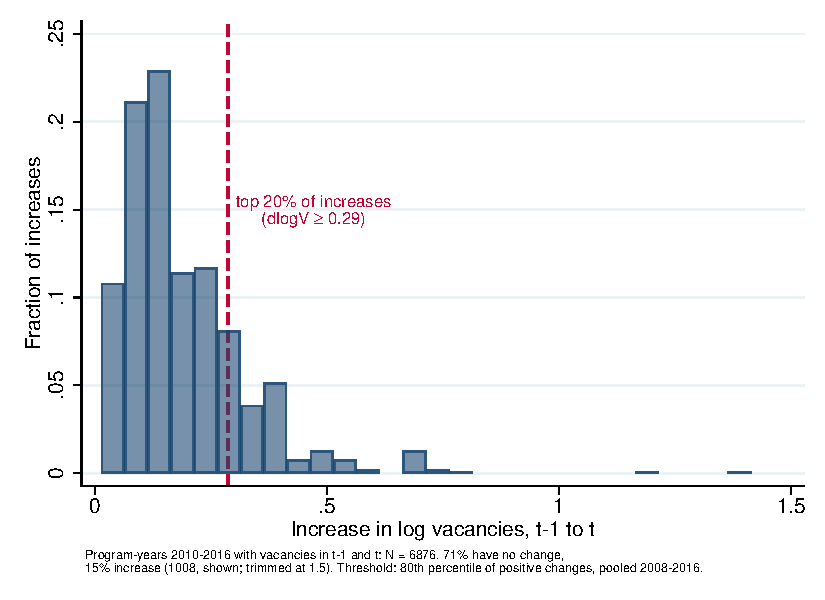
\includegraphics[width=\linewidth]{../../output/vacancy_shocks/figures/vs_dlogV_hist.pdf}
\end{column}
\begin{column}{0.46\textwidth}
\centering
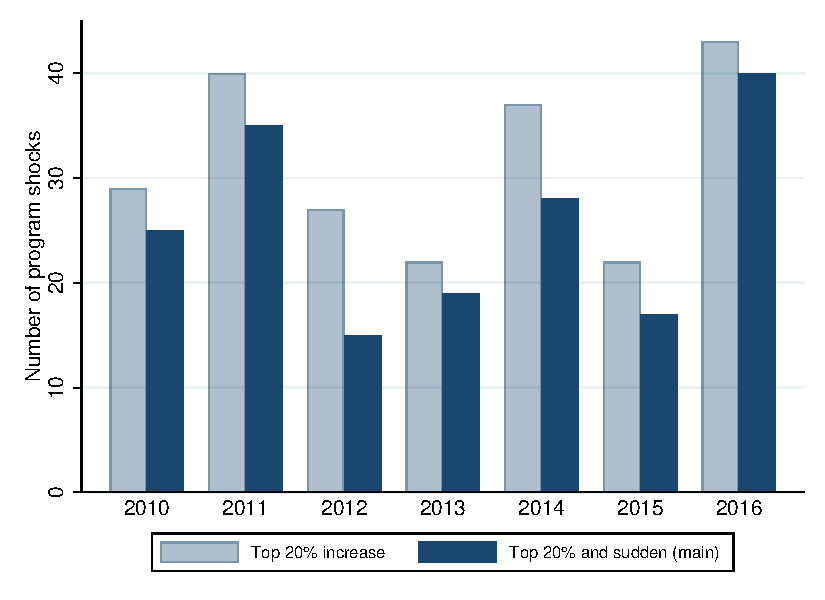
\includegraphics[width=\linewidth]{../../output/vacancy_shocks/figures/vs_shocks_by_year.pdf}
\end{column}
\end{columns}
\vspace{0.1cm}
\begin{itemize}\scriptsize
    \item 71\% of program-years have no change in regular vacancies and 15\% increase. The top-20\% threshold
    is $\Delta\log V \ge 0.29 = \log(4/3)$: vacancies are round numbers, so many increases are exactly $+33\%$.
    \item The sudden conditions remove about a fifth of top-20\% increases. Shocks are spread over 2010--2016.
\end{itemize}
\end{frame}

%--------------------------------------------------------
\begin{frame}{Design IV: where are the shocks?}
\centering
\begin{columns}[T,onlytextwidth]
\begin{column}{0.62\textwidth}
\centering
\tiny
\resizebox{\linewidth}{!}{\begin{tabular}{lrrrr}
\toprule
 & Program-years & Shocks & Shock rate (\%) & Share of shocks (\%) \\
\midrule
\multicolumn{5}{l}{\textit{Pre-period selectivity (entrant PSU quintile)}} \\
\quad No PSU data &       809 &        20 &   2.5 &  11.2 \\
\quad Q1 (least selective) &       976 &        31 &   3.2 &  17.3 \\
\quad Q2 &     1,150 &        26 &   2.3 &  14.5 \\
\quad Q3 &     1,288 &        29 &   2.3 &  16.2 \\
\quad Q4 &     1,331 &        40 &   3.0 &  22.3 \\
\quad Q5 (most selective) &     1,322 &        33 &   2.5 &  18.4 \\
\addlinespace
\multicolumn{5}{l}{\textit{Field of study}} \\
\quad Tecnología &     2,015 &        55 &   2.7 &  30.7 \\
\quad Educación &     1,441 &        36 &   2.5 &  20.1 \\
\quad Administración y Comercio &       509 &        19 &   3.7 &  10.6 \\
\quad Salud &       886 &        19 &   2.1 &  10.6 \\
\quad Ciencias Básicas &       565 &        14 &   2.5 &   7.8 \\
\quad Arte y Arquitectura &       347 &        13 &   3.7 &   7.3 \\
\quad Ciencias Sociales &       625 &        12 &   1.9 &   6.7 \\
\quad Humanidades &       157 &        10 &   6.4 &   5.6 \\
\quad Derecho &       142 &         1 &   0.7 &   0.6 \\
\quad Agropecuaria &       189 &         0 &   0.0 &   0.0 \\
\addlinespace
\multicolumn{5}{l}{\textit{University}} \\
\quad Private (CRUCH) &     2,563 &        59 &   2.3 &  33.0 \\
\quad State (CRUCH) &     4,313 &       120 &   2.8 &  67.0 \\
\addlinespace
\multicolumn{5}{l}{\textit{Year}} \\
\quad 2010 &       929 &        25 &   2.7 &  14.0 \\
\quad 2011 &       936 &        35 &   3.7 &  19.6 \\
\quad 2012 &       946 &        15 &   1.6 &   8.4 \\
\quad 2013 &       980 &        19 &   1.9 &  10.6 \\
\quad 2014 &     1,026 &        28 &   2.7 &  15.6 \\
\quad 2015 &       999 &        17 &   1.7 &   9.5 \\
\quad 2016 &     1,060 &        40 &   3.8 &  22.3 \\
\midrule
Total &     6,876 &       179 &   2.6 & 100.0 \\
\bottomrule
\end{tabular}
}
\end{column}
\begin{column}{0.36\textwidth}
\centering
\tiny
\begin{tabular}{lrr}
\toprule
Shocks per program, 2010--2016 & Programs & \% \\
\midrule
0 &     1,196 &  87.9 \\
1 &       149 &  11.0 \\
2 &        15 &   1.1 \\
\midrule
Total &     1,360 & 100.0 \\
\bottomrule
\end{tabular}


\vspace{0.3cm}
\begin{itemize}\scriptsize
    \item 88\% of programs are never shocked; shocks are almost always one-off.
    \item Shocks are spread across the selectivity distribution.
    \item More frequent at state universities and in Humanities; almost absent in Law and Agriculture.
\end{itemize}
\end{column}
\end{columns}
\end{frame}

%--------------------------------------------------------
\begin{frame}{Design IV: construction of the exposure measures}
\footnotesize
\setlength{\abovedisplayskip}{3pt}
\setlength{\belowdisplayskip}{3pt}

\textbf{1. Seats added by a shock at $j$ and pre-period market size}
\[
\text{seats}_{jt}=(V_{jt}-V_{j,t-1})\,\text{shock}_{jt},
\qquad
T_m=\sum_{\ell:\,m(\ell)=m}\overline{N}^{\mathrm{first}}_{\ell,2007\text{--}2009}.
\]
\vspace{-0.1cm}
{\scriptsize $m(\ell)$ is program $\ell$'s campus region $\times$ field market (Broad, ISCED-97 or Generic field).}

\vspace{0.10cm}
\textbf{2. Exposure of incumbent $k$ in year $t$}
\[
E^{w}_{kt}=100\times\frac{\sum_{j\in m(k),\,j\neq k} w(k,j)\,\text{seats}_{jt}}{T_{m(k)}},
\qquad
\text{cum}E^{w}_{kt}=\sum_{s=2010}^{t}E^{w}_{ks}.
\]

\vspace{-0.05cm}
\textbf{3. Weights, as in Design III ($S$ = mean entrant PSU, 2007--2009; $h=50$)}
\[
w^{\mathrm{Total}}=1,
\qquad
w^{\mathrm{Tri}}=\max\!\left(0,1-\tfrac{|S_k-S_j|}{h}\right),
\qquad
w^{\mathrm{Gau}}=\exp\!\left[-\tfrac12\left(\tfrac{|S_k-S_j|}{h}\right)^2\right].
\]

\begin{itemize}
\scriptsize
\setlength{\itemsep}{0pt}
    \item Total exposure: competitor seats added in $k$'s market, in percentage points of the market's pre-period enrollment.
    \item Kernels give more weight to shocks at programs with similar selectivity, so exposure varies within a market.
    \item $\text{cum}E_{kt}$ is the time-varying analogue of $E_p\times Post_t$ in Design III. For programs created after 2009, $S_j$ uses their first three cohorts.
\end{itemize}
\end{frame}

%--------------------------------------------------------
\begin{frame}{Design IV: samples and descriptive statistics}
\centering
\tiny
\textit{Panel A: Analytical samples}

\vspace{0.02cm}
\resizebox{0.66\textwidth}{!}{\begin{tabular}{lrrr}
\toprule
Variable & Broad & ISCED-97 & Generic \\
\midrule
Programs &       989 &       989 &       989 \\
Program-year observations &     8,925 &     8,925 &     8,925 \\
Incumbent universities &        25 &        25 &        25 \\
Markets (field \(\times\) region) &       134 &       221 &       663 \\
Markets with a shock, 2010--2016 &        46 &        61 &        70 \\
Programs exposed to a market shock &       592 &       501 &       147 \\
Mean annual enrollment, 2007--2009 &      51.7 &      51.7 &      51.7 \\
Mean PSU score, 2007--2009 &     583.9 &     583.9 &     583.9 \\
\bottomrule
\end{tabular}
}

\vspace{0.08cm}
\textit{Panel B: Cumulative exposure in 2016, by field definition}

\vspace{0.02cm}
\resizebox{0.66\textwidth}{!}{\begin{tabular}{llrrrr}
\toprule
Field definition & Exposure measure & Mean & Std. dev. & p90 & Share zero \\
\midrule
Broad & Total &   5.79 &  12.27 &  13.10 &  38.2\% \\
 & Triangular &   2.00 &   3.31 &   5.32 &  43.6\% \\
 & Gaussian &   3.90 &   6.61 &  10.46 &  38.2\% \\
\addlinespace
ISCED-97 & Total &   5.25 &   7.50 &  16.67 &  47.0\% \\
 & Triangular &   2.06 &   4.03 &   6.32 &  53.0\% \\
 & Gaussian &   3.73 &   5.90 &  11.26 &  47.0\% \\
\addlinespace
Generic & Total &   2.88 &   8.45 &  11.90 &  82.7\% \\
 & Triangular &   1.02 &   4.83 &   1.53 &  86.8\% \\
 & Gaussian &   2.07 &   6.84 &   6.99 &  82.7\% \\
\bottomrule
\end{tabular}
}

\vspace{0.06cm}
\parbox{0.94\textwidth}{\tiny
\textit{Notes:} Incumbent programs with 2007--2009 entrants and PSU data, excluding SUA entrants. Panel B reports
unweighted moments across programs of cumulative exposure in 2016, in percentage points of pre-period market
enrollment, including zero-exposure programs. Kernels use a 50-point PSU bandwidth.}
\end{frame}

%--------------------------------------------------------
\begin{frame}[label=vs-exposure-main]
\frametitle{Design IV: distribution of exposure measures
\hfill
\hyperlink{vs-exposure-appendix}{\scriptsize\color{blue}Alternative fields $\rightarrow$}}
\centering
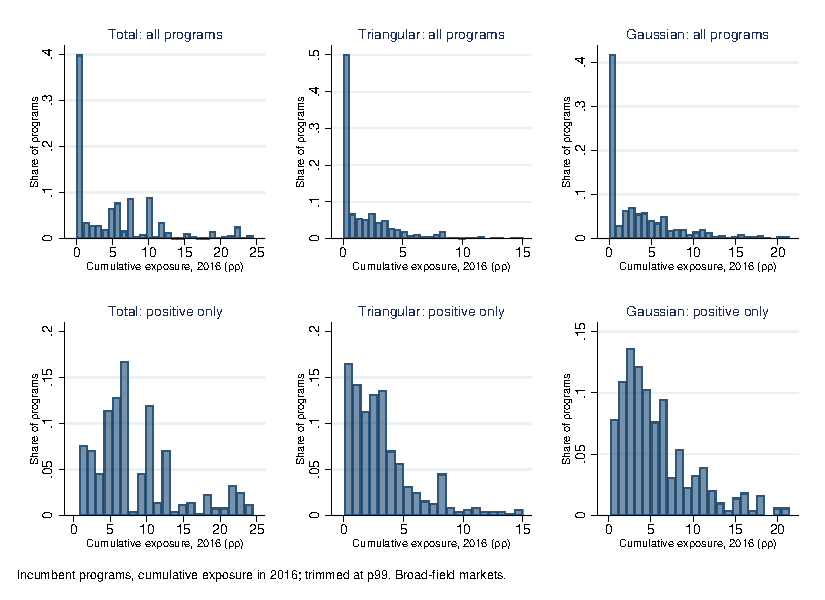
\includegraphics[width=0.80\textwidth, height=0.64\textheight, keepaspectratio]{../../output/vacancy_shocks/figures/vs_exposure_dist_broad.pdf}

\vspace{-0.10cm}
\begin{itemize}
    \scriptsize
    \setlength{\itemsep}{2pt}
    \item Each incumbent program appears once, at its cumulative exposure in 2016 (Broad-field markets).
    \item The upper row includes all programs; the lower row keeps positive exposure only.
    \item About 38\% of programs are never exposed. Triangular weighting is the most restrictive.
\end{itemize}
\end{frame}

%--------------------------------------------------------
\begin{frame}{Design IV: models to estimate}
\scriptsize
\setlength{\abovedisplayskip}{1pt}
\setlength{\belowdisplayskip}{1pt}

\textbf{(1) TWFE, levels} (mirror of the Design III first stage)

\centerline{\resizebox{0.72\textwidth}{!}{$N^{\mathrm{first}}_{kt}=\pi_w\,\text{cum}E^{w}_{kt}+\delta\,\text{Own}_{kt}+\mu_k+\alpha_{f(k),t}+\gamma_{r(k),t}+\nu_{kt}$}}

\vspace{0.06cm}
\textbf{(2) TWFE, logs}, zero exposure kept with an indicator

\centerline{\resizebox{0.92\textwidth}{!}{$\log N^{\mathrm{first}}_{kt}=\beta_w\,\widetilde{\log \text{cum}E^{w}_{kt}}+\theta_w\,\mathbf 1\{\text{cum}E^{w}_{kt}>0\}+\delta\,\text{Own}_{kt}+\mu_k+\alpha_{f(k),t}+\gamma_{r(k),t}+\varepsilon_{kt}$}}

\vspace{0.06cm}
\textbf{(3) Conditional similarity}, markets with at least one shock, using $\text{cum}E^{w}_{kt}=M_{kt}\times Q^{w}_{kt}$

\centerline{\resizebox{0.82\textwidth}{!}{$N^{\mathrm{first}}_{kt}=\beta_w\,Q^{w}_{kt}+\lambda\,\mathbf 1\{M_{kt}>0\}+\delta\,\text{Own}_{kt}+\mu_k+\alpha_{f(k),t}+\gamma_{r(k),t}+\varepsilon_{kt}$}}

\vspace{0.06cm}
\textbf{(4) Cosine exposure}: model (1) with $\text{cum}E^{d}_{kt}$, $d\in\{PSU,\ PSU\times R,\ PSU\times R\times F,\ PSU+R,\ PSU+R+F\}$.

\vspace{0.06cm}
\textbf{(5) Event studies} around $g_k$, the first year $k$ is hit (market shock; close-competitor shock; top-5 cosine shock)

\centerline{\resizebox{0.78\textwidth}{!}{$y_{kt}=\sum_{\ell\neq-1}b_\ell\,\mathbf 1\{t-g_k=\ell\}+\delta\,\text{Own}_{kt}+\mu_k+\alpha_{f(k),t}+\gamma_{r(k),t}+e_{kt}$}}

\vspace{0.06cm}
\begin{itemize}
\setlength{\itemsep}{0pt}
    \item Callaway \& Sant'Anna with two control groups: never treated only, and not-yet-treated plus never treated. Balanced panel; no field- or region-year effects.
    \item $\text{Own}_{kt}$: $k$'s own vacancy shocks to date. Market measures in 10 pp units, SE clustered by market; cosine in SD units, clustered by program.
\end{itemize}
\end{frame}

%--------------------------------------------------------
\begin{frame}[label=vs-first-stage]
\frametitle{Design IV: exposure to competitor vacancy shocks
\hfill
\hyperlink{vs-event-studies-mkt}{\scriptsize\color{blue}Event studies $\rightarrow$}}
\centering
\resizebox{0.60\textwidth}{!}{$N^{\mathrm{first}}_{kt}=\pi_w\,\text{cum}E^{w,m}_{kt}+\delta\,\text{Own}_{kt}+\mu_k+\alpha_{f_m(k),t}+\gamma_{r(k),t}+\nu_{kt}$}

\vspace{0.05cm}
\scriptsize
\resizebox{0.62\textwidth}{!}{\begin{tabular}{lcccccc}
\toprule
 & \multicolumn{3}{c}{Field \(\times\) year FE} & \multicolumn{3}{c}{\(+\) Region \(\times\) year FE} \\
\cmidrule(lr){2-4}\cmidrule(lr){5-7}
Exposure measure & Broad & ISCED-97 & Generic & Broad & ISCED-97 & Generic \\
\midrule
\textit{Total} &  0.588 &  2.413\sym{**} &  1.109 &  0.368 &  1.499\sym{*} & -0.286 \\
 & (0.677) & (0.945) & (0.874) & (0.362) & (0.786) & (0.815) \\
\quad Wald \(F\) &  0.76 &  6.51 &  1.61 &  1.03 &  3.64 &  0.12 \\
\addlinespace
\textit{Triangular} &  1.572 &  2.212 &  0.247 &  0.544 &  1.164 & -1.594 \\
 & (1.814) & (1.434) & (0.908) & (1.551) & (1.046) & (1.016) \\
\quad Wald \(F\) &  0.75 &  2.38 &  0.07 &  0.12 &  1.24 &  2.46 \\
\addlinespace
\textit{Gaussian} &  1.105 &  2.528\sym{**} &  1.064 &  0.673 &  1.536\sym{**} & -0.545 \\
 & (1.031) & (1.021) & (0.804) & (0.654) & (0.759) & (0.816) \\
\quad Wald \(F\) &  1.15 &  6.14 &  1.75 &  1.06 &  4.10 &  0.45 \\
\midrule
Observations &     8,915 &     8,913 &     8,667 &     8,915 &     8,913 &     8,667 \\
Programs &       979 &       979 &       950 &       979 &       979 &       950 \\
Markets &       134 &       221 &       631 &       134 &       221 &       631 \\
Program FE & Yes & Yes & Yes & Yes & Yes & Yes \\
Field \(\times\) year FE & Yes & Yes & Yes & Yes & Yes & Yes \\
Region \(\times\) year FE & No & No & No & Yes & Yes & Yes \\
\bottomrule
\end{tabular}
}

\vspace{0.08cm}
\parbox{0.97\textwidth}{\tiny
\textit{Notes:} The dependent variable is first-year enrollment of incumbent programs. Exposure is cumulative
competitor seats added since 2010, in 10 percentage-point units of pre-period market enrollment. All regressions
control for own shocks and absorb program and corresponding field $\times$ year fixed effects; the last three
columns add region $\times$ year fixed effects. Standard errors clustered by market.
\sym{***}~$p<0.01$, \sym{**}~$p<0.05$, \sym{*}~$p<0.10$.
Coefficients are positive and mostly insignificant: no evidence that competitor expansions take students away.}
\end{frame}

%--------------------------------------------------------
\begin{frame}[label=vs-log-first-stage]
\frametitle{Design IV: log-log specification
\hfill
\hyperlink{vs-event-studies-mkt}{\scriptsize\color{blue}Event studies $\rightarrow$}}
\centering
\scriptsize
\resizebox{0.87\textwidth}{!}{$
\log N^{\mathrm{first}}_{kt}=\beta_w\,\widetilde{\log \text{cum}E^{w}_{kt}}+\theta_w\,D^{w}_{kt}+\delta\,\text{Own}_{kt}+\mu_k+\alpha_{f(k),t}+\gamma_{r(k),t}+\varepsilon_{kt},
\quad D^{w}_{kt}=\mathbf 1\{\text{cum}E^{w}_{kt}>0\}
$}

\vspace{0.10cm}
\resizebox{0.95\textwidth}{!}{\begin{tabular}{lcccccc}
\toprule
 & \multicolumn{3}{c}{Field \(\times\) year FE} & \multicolumn{3}{c}{\(+\) Region \(\times\) year FE} \\
\cmidrule(lr){2-4}\cmidrule(lr){5-7}
Exposure measure & Broad & ISCED-97 & Generic & Broad & ISCED-97 & Generic \\
\midrule
\textit{Total} &  0.021 (0.020) &  0.026 (0.024) & -0.019 (0.030) &  0.008 (0.013) &  0.032\sym{*} (0.016) & -0.009 (0.030) \\
\quad \(F\) &  1.07 &  1.12 &  0.38 &  0.40 &  3.73 &  0.10 \\
\addlinespace
\textit{Triangular} &  0.001 (0.016) &  0.010 (0.018) & -0.013 (0.026) &  0.006 (0.017) &  0.023 (0.015) & -0.005 (0.026) \\
\quad \(F\) &  0.00 &  0.31 &  0.26 &  0.13 &  2.53 &  0.04 \\
\addlinespace
\textit{Gaussian} &  0.013 (0.014) &  0.015 (0.016) &  0.014 (0.020) &  0.009 (0.013) &  0.018 (0.016) &  0.019 (0.020) \\
\quad \(F\) &  0.87 &  0.89 &  0.48 &  0.43 &  1.30 &  0.91 \\
\midrule
Observations &     8,865 &     8,863 &     8,614 &     8,865 &     8,863 &     8,614 \\
Programs &       975 &       975 &       947 &       975 &       975 &       947 \\
\bottomrule
\end{tabular}
}

\vspace{0.10cm}
\parbox{0.94\textwidth}{\tiny
\textit{Notes:} Each coefficient is $\beta_w$, the elasticity of enrollment with respect to cumulative exposure
among exposed program-years. Zero-exposure observations are kept by setting $\widetilde{\log \text{cum}E}=0$
and including $D^{w}_{kt}$, not reported. Standard errors clustered by market. Observations with zero enrollment
are excluded. All elasticities are below 0.035 in absolute value.}
\end{frame}

%--------------------------------------------------------
\begin{frame}{Design IV: kernel-weighted denominator}
\footnotesize
\setlength{\abovedisplayskip}{3pt}
\setlength{\belowdisplayskip}{3pt}
\[
E^{w,KD}_{kt}=100\times\frac{\sum_{j\in m(k),\,j\neq k} w(k,j)\,\text{seats}_{jt}}{\sum_{\ell\in m(k)} w(k,\ell)\,\overline{N}^{\mathrm{first}}_{\ell,2007\text{--}2009}},
\qquad w\in\{\mathrm{Tri},\mathrm{Gau}\},\ \ w(k,k)=1.
\]
\vspace{-0.1cm}
\begin{itemize}
\scriptsize
\setlength{\itemsep}{1pt}
    \item Same numerator as before; the denominator is now the enrollment of programs with similar selectivity to $k$,
    not total market enrollment. As in the Design III kernel-denominator measure: for a selective $k$, the relevant
    market is the selective programs in $m(k)$.
    \item The measure keeps the scale of the shock (unlike $Q$) and lets its relevance depend on $k$'s position in the market.
\end{itemize}

\vspace{0.05cm}
\centering
\tiny
\textit{Cumulative exposure in 2016, by field definition (pp)}

\vspace{0.02cm}
\resizebox{0.78\textwidth}{!}{\begin{tabular}{llrrrrrr}
\toprule
Field definition & Exposure measure & Mean & Std. dev. & p90 & p99 & Max & Share zero \\
\midrule
Broad & Total &   5.79 &  12.27 &  13.10 &  25.54 & 298.01 &  38.2\% \\
 & Triangular KD &   4.87 &   7.11 &  12.88 &  31.24 &  67.51 &  43.6\% \\
 & Gaussian KD &   5.55 &   8.46 &  12.55 &  29.32 & 150.50 &  38.2\% \\
\addlinespace
ISCED-97 & Total &   5.25 &   7.50 &  16.67 &  31.78 &  62.50 &  47.0\% \\
 & Triangular KD &   4.55 &   7.81 &  13.43 &  32.70 &  67.51 &  53.0\% \\
 & Gaussian KD &   5.09 &   7.54 &  13.34 &  30.90 &  60.85 &  47.0\% \\
\addlinespace
Generic & Total &   2.88 &   8.45 &  11.90 &  41.47 & 100.00 &  82.7\% \\
 & Triangular KD &   1.54 &   6.13 &   3.33 &  27.10 &  96.42 &  86.8\% \\
 & Gaussian KD &   2.48 &   7.79 &   9.01 &  38.49 &  99.94 &  82.7\% \\
\bottomrule
\end{tabular}
}

\vspace{0.04cm}
\parbox{0.94\textwidth}{\tiny
\textit{Notes:} Incumbent programs, cumulative exposure in 2016, zeros included. The kernel denominator does not
generate extreme values: the maximum is below that of Total exposure in the Broad and ISCED-97 definitions.}
\end{frame}

%--------------------------------------------------------
\begin{frame}{Design IV: results with kernel-weighted denominator}
\centering
\tiny
\textit{Levels: first-year enrollment, 10 pp units}

\vspace{0.02cm}
\resizebox{0.52\textwidth}{!}{\begin{tabular}{lcccccc}
\toprule
 & \multicolumn{3}{c}{Field \(\times\) year FE} & \multicolumn{3}{c}{\(+\) Region \(\times\) year FE} \\
\cmidrule(lr){2-4}\cmidrule(lr){5-7}
Exposure measure & Broad & ISCED-97 & Generic & Broad & ISCED-97 & Generic \\
\midrule
\textit{Total} &  0.588 &  2.413\sym{**} &  1.109 &  0.368 &  1.499\sym{*} & -0.286 \\
 & (0.677) & (0.945) & (0.874) & (0.362) & (0.786) & (0.815) \\
\quad Wald \(F\) &  0.76 &  6.51 &  1.61 &  1.03 &  3.64 &  0.12 \\
\addlinespace
\textit{Triangular KD} &  1.591 &  1.359\sym{*} &  0.956 &  0.691 &  0.572 & -0.741 \\
 & (1.165) & (0.724) & (0.971) & (1.150) & (0.611) & (0.954) \\
\quad Wald \(F\) &  1.86 &  3.52 &  0.97 &  0.36 &  0.88 &  0.60 \\
\addlinespace
\textit{Gaussian KD} &  1.436 &  2.355\sym{***} &  1.367 &  0.829 &  1.425\sym{**} & -0.176 \\
 & (1.014) & (0.821) & (0.838) & (0.659) & (0.622) & (0.796) \\
\quad Wald \(F\) &  2.01 &  8.23 &  2.66 &  1.58 &  5.25 &  0.05 \\
\midrule
Observations &     8,915 &     8,913 &     8,667 &     8,915 &     8,913 &     8,667 \\
Programs &       979 &       979 &       950 &       979 &       979 &       950 \\
Markets &       134 &       221 &       631 &       134 &       221 &       631 \\
Region \(\times\) year FE & No & No & No & Yes & Yes & Yes \\
\bottomrule
\end{tabular}
}

\vspace{0.06cm}
\textit{Logs: elasticity of first-year enrollment, zero-exposure indicator included}

\vspace{0.02cm}
\resizebox{0.52\textwidth}{!}{\begin{tabular}{lcccccc}
\toprule
 & \multicolumn{3}{c}{Field \(\times\) year FE} & \multicolumn{3}{c}{\(+\) Region \(\times\) year FE} \\
\cmidrule(lr){2-4}\cmidrule(lr){5-7}
Exposure measure & Broad & ISCED-97 & Generic & Broad & ISCED-97 & Generic \\
\midrule
\textit{Total} &  0.021 &  0.026 & -0.019 &  0.008 &  0.032\sym{*} & -0.009 \\
 & (0.020) & (0.024) & (0.030) & (0.013) & (0.016) & (0.030) \\
\quad Wald \(F\) &  1.07 &  1.12 &  0.38 &  0.40 &  3.73 &  0.10 \\
\addlinespace
\textit{Triangular KD} &  0.001 &  0.007 & -0.037 & -0.004 &  0.013 & -0.028 \\
 & (0.015) & (0.017) & (0.027) & (0.016) & (0.015) & (0.028) \\
\quad Wald \(F\) &  0.01 &  0.19 &  1.88 &  0.07 &  0.80 &  1.05 \\
\addlinespace
\textit{Gaussian KD} &  0.015 &  0.015 &  0.004 &  0.005 &  0.013 &  0.008 \\
 & (0.013) & (0.016) & (0.023) & (0.011) & (0.015) & (0.023) \\
\quad Wald \(F\) &  1.36 &  0.87 &  0.03 &  0.22 &  0.75 &  0.13 \\
\midrule
Observations &     8,865 &     8,863 &     8,614 &     8,865 &     8,863 &     8,614 \\
Programs &       975 &       975 &       947 &       975 &       975 &       947 \\
Markets &       133 &       219 &       629 &       133 &       219 &       629 \\
Region \(\times\) year FE & No & No & No & Yes & Yes & Yes \\
\bottomrule
\end{tabular}
}

\vspace{0.04cm}
\parbox{0.96\textwidth}{\tiny
\textit{Notes:} Program FE, corresponding field $\times$ year FE, own shocks; region $\times$ year FE where indicated.
SE clustered by market. Total repeated for reference. Unlike Design III, where the kernel denominator turns the
weighted measures negative and significant, here they stay positive: significant only for ISCED-97 in levels
(Gaussian KD: 2.36*** and 1.43**), and all elasticities are below 0.04 in absolute value.}
\end{frame}

%--------------------------------------------------------
\begin{frame}{Design IV: kernel-weighted denominator, influence of the tail}
\centering
\scriptsize
\resizebox{0.66\textwidth}{!}{\begin{tabular}{lcccc}
\toprule
 & \multicolumn{2}{c}{Broad} & \multicolumn{2}{c}{ISCED-97} \\
\cmidrule(lr){2-3}\cmidrule(lr){4-5}
Sample & Triangular KD & Gaussian KD & Triangular KD & Gaussian KD \\
\midrule
All programs &  0.691 &  0.829 &  0.572 &  1.425\sym{**} \\
 & (1.150) & (0.659) & (0.611) & (0.622) \\
 \quad Observations &     8,915 &     8,915 &     8,913 &     8,913 \\
\addlinespace
Excluding top 1\% of exposure &  0.191 &  1.911\sym{*} &  1.043 &  2.172\sym{**} \\
 & (1.147) & (1.148) & (1.026) & (0.842) \\
 \quad Observations &     8,847 &     8,845 &     8,845 &     8,833 \\
\addlinespace
Excluding top 5\% of exposure & -2.048 &  0.688 & -0.466 &  1.937 \\
 & (1.824) & (1.597) & (1.307) & (1.353) \\
 \quad Observations &     8,530 &     8,529 &     8,516 &     8,525 \\
\bottomrule
\end{tabular}
}

\vspace{0.2cm}
\parbox{0.92\textwidth}{\tiny
\textit{Notes:} Levels, program, field $\times$ year and region $\times$ year FE, own shocks; SE clustered by market.
Programs are dropped when their cumulative KD exposure in 2016 is above the 99th or 95th percentile. Estimates move
around with the trimming, and only the Gaussian ISCED-97 estimate is significant in more than one sample; nothing
points to a negative effect.}
\end{frame}

%--------------------------------------------------------
\begin{frame}{Design IV: decomposing weighted exposure}
\scriptsize
\setlength{\abovedisplayskip}{3pt}
\setlength{\belowdisplayskip}{3pt}
\[
\text{cum}E^{w}_{kt}
=
\underbrace{\frac{\sum_{s\le t}\sum_{j\in m(k)}\text{seats}_{js}}{T_{m(k)}}}_{M_{kt}:\ \text{seats added in market}}
\times
\underbrace{\frac{\sum_{s\le t}\sum_{j\in m(k)}w(k,j)\,\text{seats}_{js}}{\sum_{s\le t}\sum_{j\in m(k)}\text{seats}_{js}}}_{Q^{w}_{kt}:\ \text{similarity with shocked programs}}
\]

\begin{columns}[T,onlytextwidth]
\begin{column}{0.47\textwidth}
\textbf{Size of competitor expansion}

\tiny
$M_{kt}$ is Total exposure: the seats added by shocks in $k$'s market up to $t$, relative to market size.
It is (almost) common to all incumbents in the market.
\end{column}
\begin{column}{0.50\textwidth}
\textbf{Conditional similarity}

\tiny
$Q^{w}_{kt}\in[0,1]$ is the seat-weighted PSU similarity between $k$ and the programs that expanded.
Conditional on the size of the expansion, it captures competitive proximity.
\end{column}
\end{columns}

\vspace{0.15cm}
\textbf{Using similarity as the independent variable}
\[
N^{\mathrm{first}}_{kt}=\beta_w\,Q^{w}_{kt}+\lambda\,\mathbf 1\{M_{kt}>0\}+\delta\,\text{Own}_{kt}+\mu_k+\alpha_{f(k),t}+\gamma_{r(k),t}+\varepsilon_{kt},
\qquad M_{k,2016}>0.
\]
\tiny
The sample is restricted to Broad-field markets with at least one shock. $Q^{w}_{kt}=0$ before the first shock in the
market, and $\mathbf 1\{M_{kt}>0\}$ absorbs the level effect of that first shock. $\beta_w$ is the enrollment change
associated with a 0.10 increase in similarity with the programs that expanded.
\end{frame}

%--------------------------------------------------------
\begin{frame}{Design IV: distribution of conditional similarity}
\centering
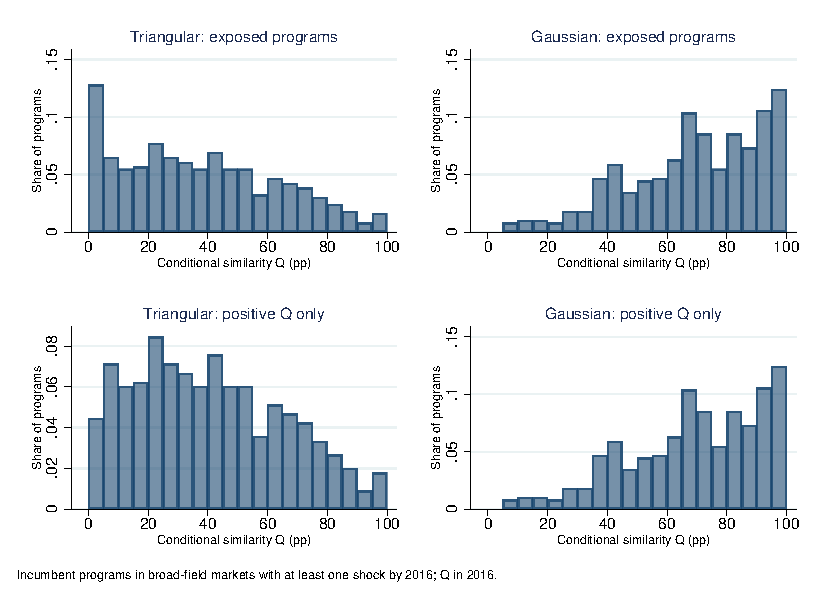
\includegraphics[width=0.74\textwidth, height=0.64\textheight, keepaspectratio]{../../output/vacancy_shocks/figures/vs_q_dist.pdf}

\vspace{-0.10cm}
\begin{itemize}
\scriptsize
\setlength{\itemsep}{2pt}
    \item Incumbent programs in Broad-field markets with at least one shock by 2016; $Q$ in 2016, in percentage points.
    \item As in Design III, the triangular measure piles up near zero and the Gaussian measure is more dispersed.
\end{itemize}
\end{frame}

%--------------------------------------------------------
\begin{frame}[label=vs-similarity-first-stage]
\frametitle{Design IV: similarity within exposed markets
\hfill
\hyperlink{vs-event-studies-close}{\scriptsize\color{blue}Event studies $\rightarrow$}}
\scriptsize
\resizebox{\textwidth}{!}{$
N^{\mathrm{first}}_{kt}=\beta_w\,Q^{w}_{kt}+\lambda\,\mathbf 1\{M_{kt}>0\}+\ldots,
\qquad
\log N^{\mathrm{first}}_{kt}=\delta_w\,\widetilde{\log Q^{w}_{kt}}+\theta_w\,\mathbf 1\{Q^{w}_{kt}>0\}+\lambda\,\mathbf 1\{M_{kt}>0\}+\ldots
$}

\vspace{0.15cm}
\centering
\resizebox{0.62\textwidth}{!}{\begin{tabular}{lcccc}
\toprule
 & \multicolumn{2}{c}{Levels} & \multicolumn{2}{c}{Logs} \\
\cmidrule(lr){2-3}\cmidrule(lr){4-5}
 & Triangular & Gaussian & Triangular & Gaussian \\
\midrule
Similarity term & -0.394 & -0.316 & -0.014 & -0.003 \\
 & (0.240) & (0.239) & (0.022) & (0.027) \\
Wald \(F\) &  2.70 &  1.74 &  0.40 &  0.01 \\
Observations &     5,576 &     5,576 &     5,562 &     5,562 \\
Programs &       592 &       592 &       592 &       592 \\
Markets &        46 &        46 &        46 &        46 \\
\bottomrule
\end{tabular}
}

\vspace{0.10cm}
\parbox{0.94\textwidth}{\tiny
\textit{Notes:} Broad-field markets with at least one shock by 2016. Levels: coefficient per 0.10 increase in $Q$.
Logs: elasticity with respect to $Q$, with zero-$Q$ observations kept through the indicator. All regressions control
for own shocks and absorb program, Broad-field $\times$ year and region $\times$ year fixed effects. Standard errors
clustered by market. The sign matches Design III (closer competitors, lower enrollment), but no estimate is significant.}
\end{frame}

%--------------------------------------------------------
\begin{frame}{Design IV: heterogeneity by incumbent selectivity}
\centering
\tiny
\begin{tabular}{lcccccc}
\toprule
 & \multicolumn{2}{c}{PSU \(<550\)} & \multicolumn{2}{c}{PSU 550--649} & \multicolumn{2}{c}{PSU \(\geq650\)} \\
\cmidrule(lr){2-3}\cmidrule(lr){4-5}\cmidrule(lr){6-7}
 & Tri. & Gau. & Tri. & Gau. & Tri. & Gau. \\
\midrule
\multicolumn{7}{l}{\textit{Vacancy-shock exposure}} \\[2pt]
Coefficient &   3.60 &   2.74 &   0.06 &  -0.01 & -23.59 & -13.51 \\
 & ( 2.73) & ( 1.92) & ( 1.23) & ( 0.42) & (28.11) & (17.80) \\
\(F\)-statistic &  1.74 &  2.03 &  0.00 &  0.00 &  0.70 &  0.58 \\
Observations & \multicolumn{2}{c}{    2,785} & \multicolumn{2}{c}{    4,783} & \multicolumn{2}{c}{    1,314} \\
Programs & \multicolumn{2}{c}{      335} & \multicolumn{2}{c}{      502} & \multicolumn{2}{c}{      139} \\
Clusters & \multicolumn{2}{c}{       95} & \multicolumn{2}{c}{       98} & \multicolumn{2}{c}{       25} \\
\midrule
\multicolumn{7}{l}{\textit{Conditional similarity \(Q\)}} \\[2pt]
Coefficient &  -0.13 &  -0.35\sym{*} &  -0.21 &  -0.05 &  -2.18 &  -4.04 \\
 & ( 0.36) & ( 0.20) & ( 0.31) & ( 0.46) & ( 2.26) & ( 3.81) \\
\(F\)-statistic &  0.13 &  2.96 &  0.44 &  0.01 &  0.94 &  1.13 \\
Observations & \multicolumn{2}{c}{    1,315} & \multicolumn{2}{c}{    3,239} & \multicolumn{2}{c}{      779} \\
Programs & \multicolumn{2}{c}{      148} & \multicolumn{2}{c}{      338} & \multicolumn{2}{c}{       83} \\
Clusters & \multicolumn{2}{c}{       24} & \multicolumn{2}{c}{       34} & \multicolumn{2}{c}{       10} \\
\bottomrule
\end{tabular}


\vspace{0.1cm}
\parbox{0.95\textwidth}{\tiny
\textit{Notes:} Incumbent PSU is the 2007--2009 mean entrant PSU. Standard errors clustered by Broad-field market.
The first panel includes program, Broad-field $\times$ year and region $\times$ year FE; the second includes program
and market $\times$ year FE and is restricted to markets with at least one shock. Coefficients correspond to a
10 percentage-point increase in exposure or a 0.10 increase in conditional similarity. Only Gaussian $Q$ among
low-PSU programs is significant (10\%); estimates for PSU $\geq650$ are very imprecise.}
\end{frame}

%--------------------------------------------------------
\begin{frame}{Design IV: cosine exposure}
\scriptsize
\setlength{\abovedisplayskip}{2pt}
\setlength{\belowdisplayskip}{2pt}
\tiny
Each program is represented by the distribution of its first-year students across 25-point PSU bins
(2007--2009 entrants; first three cohorts for later programs), as in Design III.

\vspace{0.06cm}
\textbf{1. Similarity between incumbent $k$ and source $j$}
\[
\cos\theta^{PSU}_{j,k}=\frac{\mathbf v_j\cdot\mathbf v_k}{\lVert\mathbf v_j\rVert\lVert\mathbf v_k\rVert},
\quad
\cos\theta^{PSU\times R}=\cos\theta^{PSU}\,\mathbf 1\{r_j=r_k\},
\quad
\cos\theta^{PSU\times R\times F}=\cos\theta^{PSU}\,\mathbf 1\{r_j=r_k,f_j=f_k\},
\]
\[
\cos\theta^{PSU+R}=\tfrac{\cos\theta^{PSU}+\mathbf 1\{r_j=r_k\}}{2},
\qquad
\cos\theta^{PSU+R+F}=\tfrac{\cos\theta^{PSU}+\mathbf 1\{r_j=r_k\}+\mathbf 1\{f_j=f_k\}}{3}.
\]
Each program has one campus region and one Broad field, so the interaction-cell cosines equal the PSU cosine
when programs share the region (and field), and zero otherwise.

\vspace{0.06cm}
\textbf{2. Exposure of incumbent program $k$}
\[
E^{d}_{kt}=\sum_{j\neq k} w_{jt}\cos\theta^{d}_{j,k},
\qquad
w_{jt}=\frac{\text{seats}_{jt}}{\sum_{s=2010}^{2016}\sum_{\ell}\text{seats}_{\ell s}},
\qquad
\text{cum}E^{d}_{kt}=\sum_{s=2010}^{t}E^{d}_{ks}.
\]
The weights sum to one over all 3,307 seats added by shocks in 2010--2016, as entrant enrollment weights sum to one
in Design III. In 2016, $\text{cum}E^{d}_{k}$ is $k$'s seat-weighted similarity with every program that expanded.
\end{frame}

%--------------------------------------------------------
\begin{frame}{Design IV: cosine exposure, samples and descriptive statistics}
\centering
\tiny
\textit{Panel A: Analytical samples}

\vspace{0.02cm}
\resizebox{0.60\textwidth}{!}{\begin{tabular}{lrr}
\toprule
Variable & Full sample & \(\bar N^{\mathrm{first}}_{k,2007\text{--}09}\geq10\) \\
\midrule
Programs &       989 &       943 \\
Program-year observations &     8,925 &     8,647 \\
Incumbent universities &        25 &        25 \\
Mean annual enrollment, 2007--2009 &      51.7 &      53.9 \\
Mean PSU score, 2007--2009 &     583.9 &     586.4 \\
\bottomrule
\end{tabular}
}

\vspace{0.08cm}
\textit{Panel B: Cumulative cosine exposure in 2016}

\vspace{0.02cm}
\resizebox{0.95\textwidth}{!}{\begin{tabular}{lrrrrrr}
\toprule
 & \multicolumn{3}{c}{Full sample} & \multicolumn{3}{c}{\(\bar N^{\mathrm{first}}_{k}\geq10\)} \\
\cmidrule(lr){2-4}\cmidrule(lr){5-7}
Exposure measure & Mean & Std. dev. & Share zero & Mean & Std. dev. & Share zero \\
\midrule
PSU bins & 0.4834 & 0.1203 &   0.0\% & 0.4862 & 0.1183 &   0.0\% \\
PSU bins \(\times\) campus region & 0.0858 & 0.0828 &   6.3\% & 0.0876 & 0.0829 &   6.0\% \\
PSU bins \(+\) campus region & 0.3182 & 0.0851 &   0.0\% & 0.3211 & 0.0831 &   0.0\% \\
PSU bins \(\times\) campus region \(\times\) Broad field & 0.0135 & 0.0180 &  38.2\% & 0.0137 & 0.0181 &  37.9\% \\
PSU bins \(+\) campus region \(+\) Broad field & 0.2619 & 0.0683 &   0.0\% & 0.2642 & 0.0670 &   0.0\% \\
\bottomrule
\end{tabular}
}

\vspace{0.06cm}
\parbox{0.95\textwidth}{\tiny
\textit{Notes:} The unit is an incumbent program; moments are unweighted across programs. The restricted sample
excludes programs with fewer than 10 first-year students per year in 2007--2009; the restriction is applied after
exposure construction. Multiplicative measures require coincidence in the indicated dimensions; additive measures
give equal weight to PSU similarity, campus-region coincidence and, where applicable, Broad-field coincidence.}
\end{frame}

%--------------------------------------------------------
\begin{frame}[label=vs-cosine-main]
\frametitle{Design IV: distribution of cosine exposure
\hfill
\hyperlink{vs-cosine-positive}{\scriptsize\color{blue}Positive exposure only $\rightarrow$}}
\centering
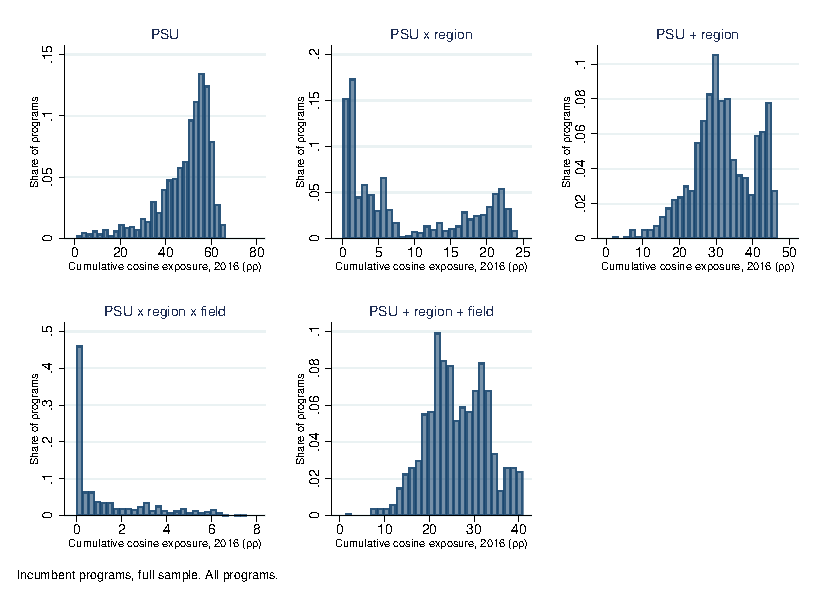
\includegraphics[width=0.82\textwidth, height=0.64\textheight, keepaspectratio]{../../output/vacancy_shocks/figures/vs_cos_dist_all.pdf}

\vspace{-0.10cm}
\begin{itemize}
\scriptsize
\setlength{\itemsep}{2pt}
    \item Each incumbent program appears once, at its cumulative cosine exposure in 2016, in percentage points.
    \item As in Design III, the multiplicative PSU $\times$ region $\times$ field measure has the most mass at zero and the smallest support.
\end{itemize}
\end{frame}

%--------------------------------------------------------
\begin{frame}[label=vs-cosine-first-stage]
\frametitle{Design IV: cosine exposure results
\hfill
\hyperlink{vs-event-studies-cos}{\scriptsize\color{blue}Event studies $\rightarrow$}}
\centering
\resizebox{0.60\textwidth}{!}{$
N^{\mathrm{first}}_{kt}=\beta_d\,\text{cum}E^{d}_{kt}+\delta\,\text{Own}_{kt}+\mu_k+\alpha_{f(k),t}+\gamma_{r(k),t}+\varepsilon_{kt}
$}

\vspace{-0.05cm}
\tiny
\resizebox{0.82\textwidth}{!}{\begin{tabular}{lcccccc}
\toprule
 & \multicolumn{3}{c}{Full sample} & \multicolumn{3}{c}{\(\bar N^{\mathrm{first}}_{k}\geq10\)} \\
\cmidrule(lr){2-4}\cmidrule(lr){5-7}
Exposure measure & \shortstack{(1)\\\(+\) year} & \shortstack{(2)\\\(+\) field\(\times\)year} & \shortstack{(3)\\\(+\) region\(\times\)year} & \shortstack{(4)\\\(+\) year} & \shortstack{(5)\\\(+\) field\(\times\)year} & \shortstack{(6)\\\(+\) region\(\times\)year} \\
\midrule
PSU bins & -3.852\sym{*} & -3.963\sym{*} & -2.447 & -4.003\sym{*} & -4.076 & -2.230 \\
 & (2.082) & (2.330) & (2.355) & (2.197) & (2.482) & (2.476) \\
\quad Wald \(F\) &  3.42 &  2.89 &  1.08 &  3.32 &  2.70 &  0.81 \\
\addlinespace
PSU bins \(\times\) region &  2.136\sym{***} &  2.305\sym{***} & -3.285 &  2.133\sym{***} &  2.344\sym{***} & -3.267 \\
 & (0.376) & (0.392) & (2.608) & (0.390) & (0.409) & (2.645) \\
\quad Wald \(F\) & 32.21 & 34.55 &  1.59 & 29.91 & 32.86 &  1.53 \\
PSU bins \(\times\) region \(\times\) field &  1.584\sym{***} &  1.969\sym{***} & -0.334 &  1.557\sym{***} &  1.965\sym{***} & -0.393 \\
 & (0.383) & (0.476) & (0.890) & (0.392) & (0.493) & (0.912) \\
\quad Wald \(F\) & 17.09 & 17.12 &  0.14 & 15.81 & 15.86 &  0.19 \\
\addlinespace
PSU bins \(+\) region &  2.629\sym{**} &  2.938\sym{**} & -3.296 &  2.701\sym{**} &  3.164\sym{**} & -3.015 \\
 & (1.139) & (1.289) & (3.048) & (1.236) & (1.417) & (3.218) \\
\quad Wald \(F\) &  5.33 &  5.20 &  1.17 &  4.77 &  4.99 &  0.88 \\
PSU bins \(+\) region \(+\) field &  2.829\sym{***} &  3.434\sym{**} & -4.000 &  2.903\sym{***} &  3.767\sym{**} & -3.673 \\
 & (0.864) & (1.524) & (3.553) & (0.923) & (1.703) & (3.812) \\
\quad Wald \(F\) & 10.72 &  5.08 &  1.27 &  9.89 &  4.89 &  0.93 \\
\midrule
Observations &     8,915 &     8,915 &     8,915 &     8,640 &     8,640 &     8,640 \\
Programs &       979 &       979 &       979 &       936 &       936 &       936 \\
\bottomrule
\end{tabular}
}

\vspace{0.04cm}
\parbox{0.97\textwidth}{\tiny
\textit{Notes:} Exposure in SD units; program-clustered standard errors. Columns (1) and (4): program and year FE;
(2) and (5): Broad-field $\times$ year FE; (3) and (6): add campus-region $\times$ year FE. Columns (4)--(6) exclude
programs with fewer than 10 first-year students per year in 2007--2009. The pattern replicates Design III: measures
that include region are positive and strongly significant until region $\times$ year FE are added, and then turn
negative and insignificant. The PSU-only measure is negative ($-3.9$, 10\%) without region $\times$ year FE.}
\end{frame}

%--------------------------------------------------------
\begin{frame}{Design IV: robustness to the shock definition}
\centering
\scriptsize
\resizebox{\textwidth}{!}{\begin{tabular}{l*{8}{c}}
\toprule
 & Main & Top 10\% & Top 25\% & Within-year & No sudden & Levels & INDICES & Admissions \\
\midrule
\textit{Total} &  0.368 &  0.269 &  0.230 &  0.440 &  0.471 &  0.352 &  0.180 &  0.964 \\
 & (0.362) & (0.289) & (0.317) & (0.414) & (0.415) & (0.387) & (0.270) & (0.989) \\
\addlinespace
\textit{Gaussian} &  0.673 &  0.657 &  0.614 &  0.866 &  0.765 &  1.069 & -0.054 & -0.774 \\
 & (0.654) & (0.710) & (0.654) & (0.725) & (0.648) & (0.814) & (0.486) & (1.348) \\
\addlinespace
\textit{Gaussian KD} &  0.829 &  1.012 &  0.832 &  1.119 &  0.855 &  1.517 &  0.189 & -0.782 \\
 & (0.659) & (0.820) & (0.673) & (0.809) & (0.634) & (0.995) & (0.447) & (1.391) \\
\midrule
Observations &     8,915 &     8,915 &     8,915 &     8,915 &     8,915 &     8,915 &     8,915 &     8,915 \\
\bottomrule
\end{tabular}
}

\vspace{0.3cm}
\resizebox{0.75\textwidth}{!}{\begin{tabular}{llrrr}
\toprule
Definition & & Shocks & Mean \(\Delta\log V\) & Mean seats added \\
\midrule
Main & top 20\%, sudden &       179 &  0.39 &   18.5 \\
Top 10\% & sudden &        79 &  0.50 &   24.4 \\
Top 25\% & sudden &       205 &  0.37 &   18.8 \\
Within-year p80 & sudden &       188 &  0.38 &   18.3 \\
No sudden conditions & top 20\% &       220 &  0.39 &   18.5 \\
Level change & top 20\% of \(\Delta V\) &       152 &  0.35 &   25.4 \\
INDICES vacancies & top 20\%, sudden &       127 &  0.40 &   21.1 \\
Admissions as vacancies & top 20\%, sudden &       319 &  0.52 &   16.8 \\
\bottomrule
\end{tabular}
}

\vspace{0.2cm}
\parbox{0.95\textwidth}{\tiny
\textit{Notes:} Specification (1), Broad-field markets, with program, field $\times$ year and region $\times$ year FE
and own shocks; standard errors clustered by market. Exposure rebuilt under each shock definition; Gaussian KD uses
the kernel-weighted denominator. No definition
delivers a significant effect.}
\end{frame}

%--------------------------------------------------------
\begin{frame}{Design IV: event studies, cohorts and pre-trend tests}
\centering
\begin{columns}[T,onlytextwidth]
\begin{column}{0.46\textwidth}
\centering
\tiny
\textbf{Treatment cohorts (programs in 2016)}

\vspace{0.05cm}
\resizebox{\linewidth}{!}{\begin{tabular}{lrrr}
\toprule
First treatment year & Market shock & Close shock & Top-5 cosine shock \\
\midrule
Never treated &    304 &    347 &    460 \\
2010 &    235 &    153 &     51 \\
2011 &    130 &    136 &     70 \\
2012 &     50 &     42 &     28 \\
2013 &     21 &     48 &     34 \\
2014 &     16 &     23 &     44 \\
2015 &     11 &     13 &     45 \\
2016 &     29 &     34 &     64 \\
\midrule
Programs &    796 &    796 &    796 \\
\bottomrule
\end{tabular}
}
\end{column}
\begin{column}{0.53\textwidth}
\centering
\tiny
\textbf{Joint pre-trend tests, $p$-values}

\vspace{0.05cm}
\resizebox{\linewidth}{!}{\begin{tabular}{llccc}
\toprule
 & & & \multicolumn{2}{c}{Callaway--Sant'Anna} \\
\cmidrule(lr){4-5}
Treatment & Outcome & TWFE & Never treated & Not yet treated \\
\midrule
Market shock & Enrollment & 0.348 & 0.080 & 0.081 \\
 & Log enrollment & 0.124 & 0.011 & 0.012 \\
\addlinespace
Close-competitor shock & Enrollment & 0.539 & 0.000 & 0.000 \\
 & Log enrollment & 0.240 & 0.000 & 0.000 \\
\addlinespace
Top-5 cosine shock & Enrollment & 0.293 & 0.021 & 0.021 \\
 & Log enrollment & 0.150 & 0.068 & 0.069 \\
\bottomrule
\end{tabular}
}
\end{column}
\end{columns}

\vspace{0.2cm}
\begin{itemize}\scriptsize
    \item Callaway \& Sant'Anna is estimated twice: with never-treated programs as the only controls, and with
    not-yet-treated plus never-treated programs. Between 38\% and 58\% of programs are never treated, so both are
    feasible; they give nearly identical estimates.
    \item TWFE (with field- and region-year FE) never rejects parallel pre-trends. CS rejects for the close-competitor
    shock and, at 5\%, for log enrollment after a market shock and enrollment after a cosine shock.
    \item After a close-competitor or market shock, CS shows enrollment \emph{rising} by 2--4 students; TWFE, which
    absorbs field- and region-year shocks, is flat. After a shock at a top-5 cosine program, both point to declines of 1--3 students, imprecisely estimated.
    \item These event studies use a binary first-shock indicator and discard the dose. The next two slides keep it.
\end{itemize}
\end{frame}

%--------------------------------------------------------
\begin{frame}{Design IV: event studies with the treatment dose}
\scriptsize
Distributed-lag event study with binned endpoints (Schmidheiny \& Siegloch 2023) on the yearly exposure flow $E_{kt}$ (10 pp):
\[
\resizebox{0.95\textwidth}{!}{$
y_{kt} = \beta_{\le -5}\sum_{s\ge t+5}E_{ks} + \sum_{l=-4}^{-2}\beta_l E_{k,t-l} + \sum_{l=0}^{3}\beta_l E_{k,t-l}
+ \beta_{\ge 4}\sum_{s\le t-4}E_{ks} + \delta\,\text{Own}_{kt} + \mu_k + \alpha_{f(k),t} + \gamma_{r(k),t} + \varepsilon_{kt}
$}
\]
$E_{k,t+1}$ is omitted, so $\beta_l$ is the cumulative effect at event time $l$ of 10 pp of exposure received at $l=0$, relative to $l=-1$.

\vspace{0.1cm}
\centering
\begin{columns}[T,onlytextwidth]
\begin{column}{0.49\textwidth}
\centering \tiny First-year enrollment

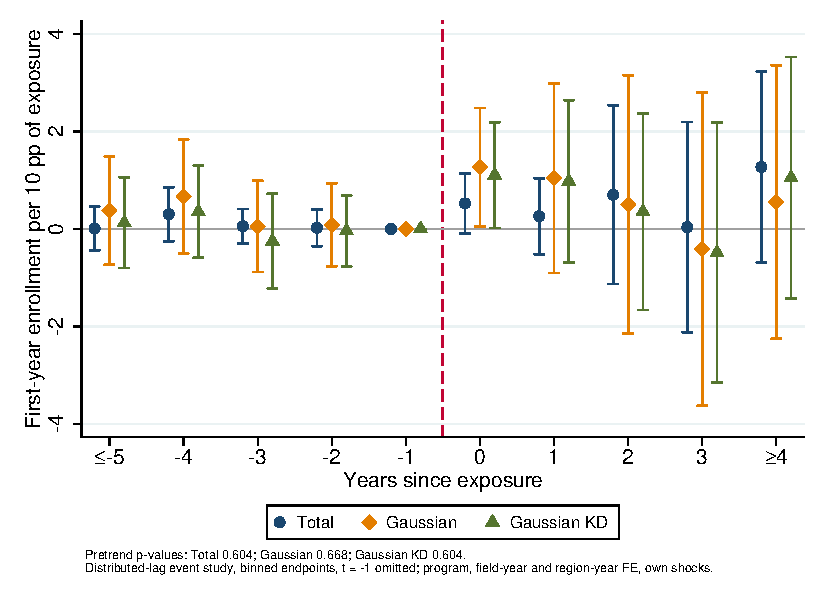
\includegraphics[width=\linewidth]{../../output/vacancy_shocks/figures/vs_esd_N_first_fr.pdf}
\end{column}
\begin{column}{0.49\textwidth}
\centering \tiny Log first-year enrollment

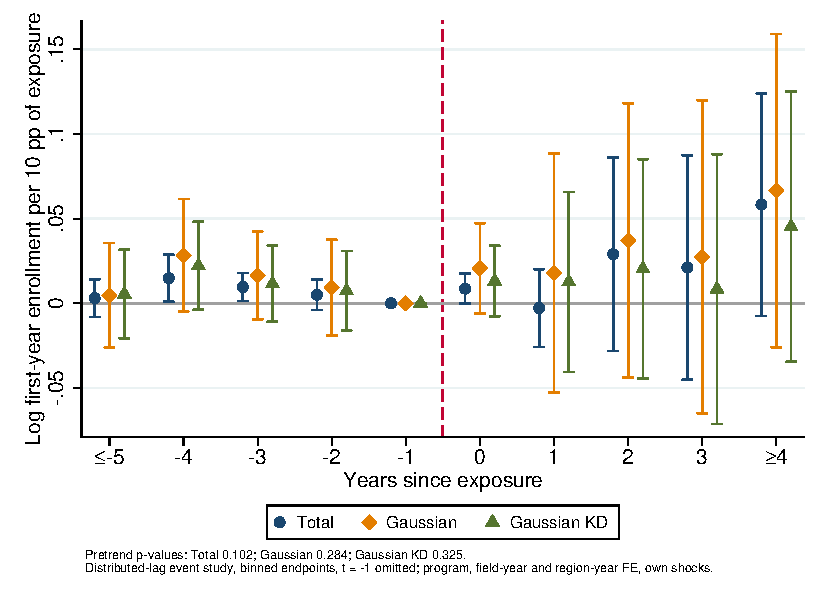
\includegraphics[width=\linewidth]{../../output/vacancy_shocks/figures/vs_esd_lnN_fr.pdf}
\end{column}
\end{columns}

\vspace{0.05cm}
\parbox{0.96\textwidth}{\tiny
\textit{Notes:} Broad field $\times$ region market; program, field $\times$ year and region $\times$ year FE, own shocks; SE clustered by market.
Leads beyond 2016 set to zero, as in the binary event studies.}
\end{frame}

%--------------------------------------------------------
\begin{frame}{Design IV: dose event studies, average post-exposure effect}
\begin{columns}[T,onlytextwidth]
\begin{column}{0.4\textwidth}
\centering
\resizebox{\linewidth}{!}{\begin{tabular}{lcccc}
\toprule
 & \multicolumn{2}{c}{Enrollment} & \multicolumn{2}{c}{Log enrollment} \\
\cmidrule(lr){2-3}\cmidrule(lr){4-5}
 & (1) & (2) & (3) & (4) \\
\midrule
\multicolumn{5}{l}{\textit{A. All years (2007--2016)}} \\
Total &  0.890 &  0.383 & 0.0286 & 0.0140 \\
 & ( 0.665) & ( 0.547) & (0.0228) & (0.0162) \\
 & [0.524] & [0.604] & [0.083] & [0.102] \\
Gaussian &  0.928 &  0.600 & 0.0318 & 0.0258 \\
 & ( 0.979) & ( 0.940) & (0.0337) & (0.0274) \\
 & [0.824] & [0.668] & [0.618] & [0.284] \\
Gaussian KD &  0.978 &  0.490 & 0.0258 & 0.0136 \\
 & ( 0.763) & ( 0.762) & (0.0268) & (0.0218) \\
 & [0.733] & [0.604] & [0.610] & [0.325] \\
Triangular KD &  0.786 &  0.376 & 0.0078 & 0.0002 \\
 & ( 1.142) & ( 1.183) & (0.0315) & (0.0290) \\
 & [0.352] & [0.608] & [0.145] & [0.881] \\
Observations &     8,915 &     8,915 &     8,865 &     8,865 \\
\midrule
\multicolumn{5}{l}{\textit{B. Years 2007--2012 (all leads observed)}} \\
Total &  1.170 &  1.795 & 0.0537 & 0.0251 \\
 & ( 1.506) & ( 1.404) & (0.0439) & (0.0403) \\
 & [0.382] & [0.091] & [0.310] & [0.055] \\
Gaussian &  0.767 &  2.308 & 0.0312 & 0.0255 \\
 & ( 1.837) & ( 1.995) & (0.0608) & (0.0622) \\
 & [0.381] & [0.200] & [0.203] & [0.162] \\
Gaussian KD &  0.838 &  1.773 & 0.0263 & 0.0072 \\
 & ( 1.457) & ( 1.654) & (0.0445) & (0.0466) \\
 & [0.371] & [0.450] & [0.174] & [0.291] \\
Triangular KD &  0.046 &  0.653 & -0.0070 & -0.0173 \\
 & ( 1.306) & ( 1.424) & (0.0422) & (0.0453) \\
 & [0.821] & [0.018] & [0.198] & [0.933] \\
Observations &     5,555 &     5,555 &     5,532 &     5,532 \\
\midrule
Field-year FE & Yes & Yes & Yes & Yes \\
Region-year FE & No & Yes & No & Yes \\
\bottomrule
\end{tabular}
}
\end{column}
\begin{column}{0.57\textwidth}
\tiny
\textit{Notes:} Coefficient: average of $\beta_0,\dots,\beta_3$ per 10 pp of exposure (SE in parentheses);
$p$-value of the joint test $\beta_{\le -5}=\beta_{-4}=\beta_{-3}=\beta_{-2}=0$ in brackets.
Panel B keeps years up to 2012, where every interior lead is observed. Program FE, field $\times$ year FE, own shocks;
SE clustered by market.

\vspace{0.2cm}
\begin{itemize}\scriptsize
    \item Keeping the dose, pre-trends are not rejected at 5\% for any measure in the full sample, unlike the binary CS event studies (which also lack field- and region-year FE). In panel B, one of 16 tests rejects (Triangular KD, $p=0.018$).
    \item Post-exposure effects are positive and insignificant (0.4--1 students per 10 pp; below 3\% in logs), consistent with the static first stages. No sign of business stealing.
\end{itemize}
\end{column}
\end{columns}
\end{frame}

%--------------------------------------------------------
% DESIGN IV: SELECTIVE VS SELECTIVE (issue #3)
%--------------------------------------------------------
\begin{frame}{Design IV, selective vs selective: question and construction}
\scriptsize
\setlength{\abovedisplayskip}{2pt}
\setlength{\belowdisplayskip}{2pt}
\textbf{Research question}

When a \emph{selective} program suddenly expands its seats, what happens to its \emph{selective} competitors?

\vspace{0.08cm}
\textbf{Construction}: Design IV objects, restricted on both sides
\begin{itemize}
    \item Incumbents $k$: the 169 selective incumbents (top 20\% of 2007--2009 entrant PSU, as in Design II).
    \item Sources $j$: selective programs only (same cutoff on $S_j$). There are 35 main shocks at selective programs.
    \item Denominator: pre-period enrollment of the \emph{selective} programs in $k$'s market,
\end{itemize}
\[
E^{w,sel}_{kt}=100\times\frac{\sum_{j\in m(k),\,j\neq k,\,j\ \text{sel.}} w(k,j)\,\text{seats}_{jt}}{\sum_{\ell\in m(k),\,\ell\ \text{sel.}}\overline{N}^{\mathrm{first}}_{\ell,2007\text{--}2009}},
\qquad \text{cum}E^{w,sel}_{kt}=\sum_{s=2010}^{t}E^{w,sel}_{ks}.
\]
\textbf{Model}: Design IV model (1) and event study around the first selective-competitor shock in $k$'s broad market.

\vspace{0.05cm}
\centering
\tiny
\resizebox{0.62\textwidth}{!}{\begin{tabular}{llccccc}
\toprule
Field & Kernel & Exposed (\%) & Mean & P50 exposed & P90 exposed & Max \\
\midrule
Broad & Total & 52.7 &  4.76 &  6.06 & 18.67 & 38.64 \\
 & Triangular & 49.1 &  2.24 &  3.02 & 10.27 & 23.98 \\
 & Gaussian & 52.7 &  3.70 &  4.67 & 15.56 & 35.96 \\
ISCED-97 & Total & 45.6 &  4.85 &  6.11 & 21.03 & 42.74 \\
 & Triangular & 41.4 &  2.33 &  2.73 & 14.97 & 23.98 \\
 & Gaussian & 45.6 &  3.84 &  4.80 & 18.81 & 36.84 \\
Generic & Total & 10.7 &  2.24 & 20.12 & 38.64 & 46.63 \\
 & Triangular &  8.3 &  0.91 &  9.06 & 23.98 & 24.00 \\
 & Gaussian & 10.7 &  1.66 & 16.07 & 30.30 & 35.96 \\
\bottomrule
\end{tabular}
}

\vspace{0.03cm}
\parbox{0.9\textwidth}{\tiny Cumulative exposure in 2016, selective incumbents, pp of selective-market enrollment. 89 of 169 selective incumbents are exposed by 2016 (broad market).}
\end{frame}

%--------------------------------------------------------
\begin{frame}{Design IV, selective vs selective: results}
\centering
\resizebox{0.62\textwidth}{!}{$N^{\mathrm{first}}_{kt}=\pi_w\,\text{cum}E^{w,sel}_{kt}+\delta\,\text{Own}_{kt}+\mu_k+\alpha_{f(k),t}+\gamma_{r(k),t}+\nu_{kt}$}

\vspace{0.05cm}
\tiny
\textit{Panel A: First-year enrollment}

\resizebox{0.66\textwidth}{!}{\begin{tabular}{lcccccc}
\toprule
 & \multicolumn{3}{c}{Field \(\times\) year FE} & \multicolumn{3}{c}{\(+\) Region \(\times\) year FE} \\
\cmidrule(lr){2-4}\cmidrule(lr){5-7}
Exposure measure & Broad & ISCED-97 & Generic & Broad & ISCED-97 & Generic \\
\midrule
\textit{Total} &  -1.740 &  -2.928\sym{**} &  -1.260 &  -1.871 &  -2.879\sym{*} &  -0.938 \\
 & ( 1.744) & ( 1.313) & ( 1.823) & ( 1.792) & ( 1.583) & ( 1.464) \\
\textit{Triangular} & -12.038\sym{**} & -12.874\sym{**} &  -9.999\sym{**} & -13.742\sym{**} & -13.542\sym{**} &  -7.526\sym{**} \\
 & ( 5.034) & ( 4.810) & ( 4.075) & ( 6.242) & ( 5.384) & ( 3.102) \\
\textit{Gaussian} &  -6.697\sym{**} &  -6.428\sym{**} &  -5.229\sym{*} &  -8.529\sym{**} &  -6.953\sym{**} &  -3.946\sym{*} \\
 & ( 2.817) & ( 2.493) & ( 2.783) & ( 3.752) & ( 2.896) & ( 2.171) \\
\midrule
Observations &  1,883 &  1,853 &  1,561 &  1,873 &  1,843 &  1,551 \\
Markets (clusters) &     31 &     45 &     98 &     30 &     44 &     97 \\
\bottomrule
\end{tabular}
}

\vspace{0.04cm}
\textit{Panel B: Log first-year enrollment}

\resizebox{0.66\textwidth}{!}{\begin{tabular}{lcccccc}
\toprule
 & \multicolumn{3}{c}{Field \(\times\) year FE} & \multicolumn{3}{c}{\(+\) Region \(\times\) year FE} \\
\cmidrule(lr){2-4}\cmidrule(lr){5-7}
Exposure measure & Broad & ISCED-97 & Generic & Broad & ISCED-97 & Generic \\
\midrule
\textit{Total} &   0.013 &   0.012 &  -0.013 &  -0.002 &   0.007 &  -0.010 \\
 & ( 0.013) & ( 0.010) & ( 0.025) & ( 0.013) & ( 0.010) & ( 0.028) \\
\textit{Triangular} &  -0.019 &  -0.012 &  -0.035 &  -0.040 &  -0.020 &  -0.024 \\
 & ( 0.035) & ( 0.030) & ( 0.028) & ( 0.043) & ( 0.034) & ( 0.029) \\
\textit{Gaussian} &   0.001 &   0.005 &  -0.022 &  -0.018 &  -0.001 &  -0.016 \\
 & ( 0.017) & ( 0.014) & ( 0.022) & ( 0.019) & ( 0.015) & ( 0.022) \\
\midrule
Observations &  1,882 &  1,853 &  1,560 &  1,872 &  1,843 &  1,550 \\
Markets (clusters) &     31 &     45 &     98 &     30 &     44 &     97 \\
\bottomrule
\end{tabular}
}

\vspace{0.04cm}
\parbox{0.97\textwidth}{\tiny
\textit{Notes:} Exposure in 10 pp units. All regressions control for own shocks. SE clustered by market.
\sym{***}~$p<0.01$, \sym{**}~$p<0.05$, \sym{*}~$p<0.10$.
In levels, the kernel measures are negative and significant: closer selective competitors expanding lowers $k$'s enrollment by about
12 entrants per 10 pp (triangular). The log specification is null, and there are only about 30 broad markets.}
\end{frame}

%--------------------------------------------------------
\begin{frame}{Design IV, selective vs selective: event study and composition}
\begin{columns}[T,onlytextwidth]
\begin{column}{0.50\textwidth}
\centering
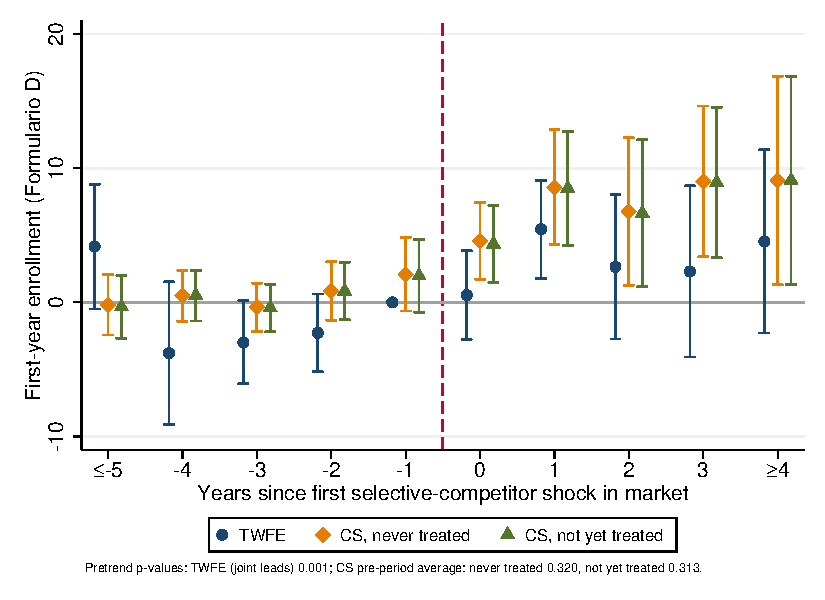
\includegraphics[width=\linewidth]{../../output/own_expansion/figures/oe_sel_es_N_first.pdf}
\end{column}
\begin{column}{0.48\textwidth}
\centering
\tiny
\resizebox{\linewidth}{!}{\begin{tabular}{lcccc}
\toprule
 & \multicolumn{2}{c}{Total} & \multicolumn{2}{c}{Gaussian} \\
\cmidrule(lr){2-3}\cmidrule(lr){4-5}
Outcome & Field-year & \(+\) Region-year & Field-year & \(+\) Region-year \\
\midrule
Mean LM PSU, entrants &   3.299\sym{**} &   1.001 &   2.945\sym{*} &  -0.447 \\
 & ( 1.361) & ( 1.588) & ( 1.706) & ( 2.081) \\
LM PSU of the last admitted &   4.976 &   5.177 &   5.047 &   4.602 \\
 & ( 3.094) & ( 4.597) & ( 3.772) & ( 5.552) \\
SD of LM PSU, entrants &  -2.751\sym{**} &  -1.706 &  -3.036\sym{*} &  -1.563 \\
 & ( 1.233) & ( 1.159) & ( 1.492) & ( 1.255) \\
Mean NEM, entrants &  -5.283 &  -1.470 &  -7.406\sym{*} &  -2.969 \\
 & ( 3.156) & ( 2.436) & ( 3.988) & ( 3.568) \\
Female, entrants, pct. &   0.347 &  -0.031 &   0.147 &  -0.240 \\
 & ( 0.665) & ( 0.889) & ( 0.833) & ( 1.237) \\
Private-paid school, entrants, pct. &  -0.001 &   0.688 &   0.160 &   0.947 \\
 & ( 0.800) & ( 0.479) & ( 1.054) & ( 0.669) \\
Municipal school, entrants, pct. &   0.420 &   0.479 &  -0.185 &  -0.470 \\
 & ( 0.690) & ( 0.984) & ( 0.867) & ( 1.175) \\
\bottomrule
\end{tabular}
}
\end{column}
\end{columns}

\vspace{0.1cm}
\begin{itemize}\scriptsize
    \setlength{\itemsep}{2pt}
    \item The event study does not support the negative level effect. Callaway--Sant'Anna gives a \emph{positive} ATT
    ($+8.7$, SE 2.5, never treated; pre-period average $p=0.32$), and the TWFE leads reject ($p=0.001$).
    \item Composition (broad market, Total and Gaussian): mean entrant PSU rises by about 3 points with field $\times$ year FE, and the effect disappears with region $\times$ year FE.
    \item Taken together, there is no robust evidence that selective expansions take students away from selective competitors.
\end{itemize}
\end{frame}

%====================================================
\section{Composition Effects}
%====================================================
\begin{frame}{Composition effects: who enters when capacity changes?}
\scriptsize
\begin{itemize}
    \item Designs I--IV ask whether capacity changes move \emph{how many} students enter a program. Here we ask whether they change \emph{who} enters.
    \item The dependent variable is the mean characteristic of the entering cohort (Formulario D entrants, program $\times$ year), not enrollment:
    \begin{itemize}
        \item Mean and SD of LM PSU, mean NEM.
        \item LM PSU of the \textbf{last admitted} (lowest application score among regular admits, status 24).
        \item Share female; shares from private-paid and municipal schools (SES proxy).
    \end{itemize}
    \item \textbf{Income is not available}: Formulario A has no income and the DEMRE socioeconomic questionnaire is not in the data.
    Income of the last admitted is replaced by the school type of the last admitted.
    \item Each design keeps its own specification, with only the outcome replaced.
    Design II and the selective-vs-selective variant of Design IV are reported in their own sections.
\end{itemize}
\end{frame}

%--------------------------------------------------------
\begin{frame}{Composition effects: Design I (FD-IV with $\Delta$ cupos)}
\centering
\resizebox{0.55\textwidth}{!}{$\Delta y^{comp}_{pt}=\beta\,\widehat{\Delta N}_{pt}+\alpha_t+\varepsilon_{pt},\qquad \Delta N_{pt}=\pi\,\Delta Z_{pt}+\alpha_t+\nu_{pt}$}

\vspace{0.08cm}
\tiny
\resizebox{0.78\textwidth}{!}{\begin{tabular}{lcccc}
\toprule
 & \multicolumn{2}{c}{2007--2012} & \multicolumn{2}{c}{2013--2016} \\
\cmidrule(lr){2-3}\cmidrule(lr){4-5}
Outcome (\(\Delta\)) & Reduced form & 2SLS & Reduced form & 2SLS \\
\midrule
First stage: \(\Delta N\) on \(\Delta Z\) &  0.695\sym{***} &  &  0.624\sym{***} &  \\
 & (0.044) &  & (0.039) &  \\
\addlinespace
Mean LM PSU, entrants &  -1.742\sym{***} &  -2.505\sym{***} &  -0.829\sym{***} &  -1.328\sym{***} \\
 & ( 0.159) & ( 0.330) & ( 0.162) & ( 0.278) \\
LM PSU of the last admitted &  -3.264\sym{***} &  -4.696\sym{***} &  -1.570\sym{***} &  -2.515\sym{***} \\
 & ( 0.550) & ( 0.919) & ( 0.501) & ( 0.807) \\
SD of LM PSU, entrants &   0.191\sym{**} &   0.275\sym{**} &  -0.143\sym{*} &  -0.229\sym{*} \\
 & ( 0.087) & ( 0.134) & ( 0.084) & ( 0.138) \\
Mean NEM, entrants &  -2.150\sym{***} &  -3.092\sym{***} &  -1.889\sym{***} &  -3.026\sym{***} \\
 & ( 0.274) & ( 0.517) & ( 0.268) & ( 0.508) \\
Female, entrants, pct. &   0.045 &   0.064 &  -0.074 &  -0.118 \\
 & ( 0.109) & ( 0.157) & ( 0.098) & ( 0.157) \\
Private-paid school, entrants, pct. &  -0.087 &  -0.125 &  -0.266\sym{***} &  -0.427\sym{***} \\
 & ( 0.089) & ( 0.124) & ( 0.086) & ( 0.139) \\
Municipal school, entrants, pct. &  -0.039 &  -0.055 &   0.006 &   0.010 \\
 & ( 0.117) & ( 0.168) & ( 0.081) & ( 0.129) \\
\midrule
Observations (FD) & \multicolumn{2}{c}{ 3,510} & \multicolumn{2}{c}{ 3,014} \\
\bottomrule
\end{tabular}
}

\vspace{0.06cm}
\parbox{0.95\textwidth}{\tiny
\textit{Notes:} $N$: enrollees with \texttt{enrolls\_target}$=1$; $Z$: total cupos. Both are in tens, so 2SLS is the effect of 10 more entrants.
Year FE, SE clustered by program. The first stage differs from the Design I frame (0.82 / 0.54) because the
sample is not restricted to cohorts with graduation outcomes.
Ten more entrants lower mean entrant PSU by 1.3--2.5 points and the last admitted's PSU by 2.5--4.7 points:
programs that expand reach further down the score distribution.}
\end{frame}

%--------------------------------------------------------
\begin{frame}{Composition effects: Design III (SUA entry)}
\begin{columns}[T,onlytextwidth]
\begin{column}{0.56\textwidth}
\centering
\tiny
\resizebox{\linewidth}{!}{\begin{tabular}{lcccccc}
\toprule
 & \multicolumn{3}{c}{Field \(\times\) year FE} & \multicolumn{3}{c}{\(+\) Region \(\times\) year FE} \\
\cmidrule(lr){2-4}\cmidrule(lr){5-7}
Outcome & Total & Triangular & Gaussian & Total & Triangular & Gaussian \\
\midrule
First-year enrollment &   1.967\sym{***} &   0.935 &   1.775\sym{***} &   0.798 &  -5.252\sym{**} &  -2.767\sym{*} \\
 & ( 0.336) & ( 0.972) & ( 0.439) & ( 0.662) & ( 2.115) & ( 1.401) \\
\addlinespace
Mean LM PSU, entrants &  -2.160\sym{***} &  -5.454\sym{***} &  -3.794\sym{***} &   0.590 &   0.162 &  -0.475 \\
 & ( 0.390) & ( 1.435) & ( 0.573) & ( 0.662) & ( 1.496) & ( 0.769) \\
LM PSU of the last admitted &  -3.063\sym{***} & -10.221\sym{***} &  -5.990\sym{***} &   0.991 &  -2.931 &  -1.749 \\
 & ( 0.513) & ( 2.356) & ( 0.918) & ( 0.964) & ( 2.627) & ( 1.281) \\
SD of LM PSU, entrants &   0.670\sym{***} &   2.180\sym{***} &   1.343\sym{***} &  -0.579\sym{**} &   0.362 &   0.267 \\
 & ( 0.152) & ( 0.402) & ( 0.236) & ( 0.245) & ( 0.483) & ( 0.307) \\
Mean NEM, entrants &   0.376 &  -5.254\sym{*} &  -2.090 &   1.925 &  -8.043\sym{**} &  -5.279\sym{**} \\
 & ( 0.659) & ( 2.868) & ( 1.396) & ( 1.324) & ( 3.815) & ( 2.142) \\
Female, entrants, pct. &   0.025 &  -0.498 &  -0.166 &   0.131 &  -0.682 &  -0.369 \\
 & ( 0.107) & ( 0.773) & ( 0.336) & ( 0.257) & ( 0.930) & ( 0.517) \\
Private-paid school, entrants, pct. &  -0.203\sym{**} &  -0.065 &  -0.151 &  -0.120 &   0.657 &   0.401\sym{*} \\
 & ( 0.094) & ( 0.281) & ( 0.136) & ( 0.163) & ( 0.414) & ( 0.205) \\
Municipal school, entrants, pct. &   0.500\sym{***} &   0.763 &   0.636\sym{**} &   0.323 &  -0.767 &  -0.345 \\
 & ( 0.163) & ( 0.594) & ( 0.322) & ( 0.317) & ( 0.470) & ( 0.345) \\
\midrule
Observations &  8,041 &  8,041 &  8,041 &  8,038 &  8,038 &  8,038 \\
\bottomrule
\end{tabular}
}

\vspace{0.05cm}
\parbox{\linewidth}{\tiny
\textit{Notes:} Levels first stage of Design III ($10\times E_p\times\text{Post}_t$), broad area $\times$ region markets, SE clustered by market.
The enrollment row reproduces the Design III estimate ($\pi=1.97$).}
\end{column}
\begin{column}{0.42\textwidth}
\centering
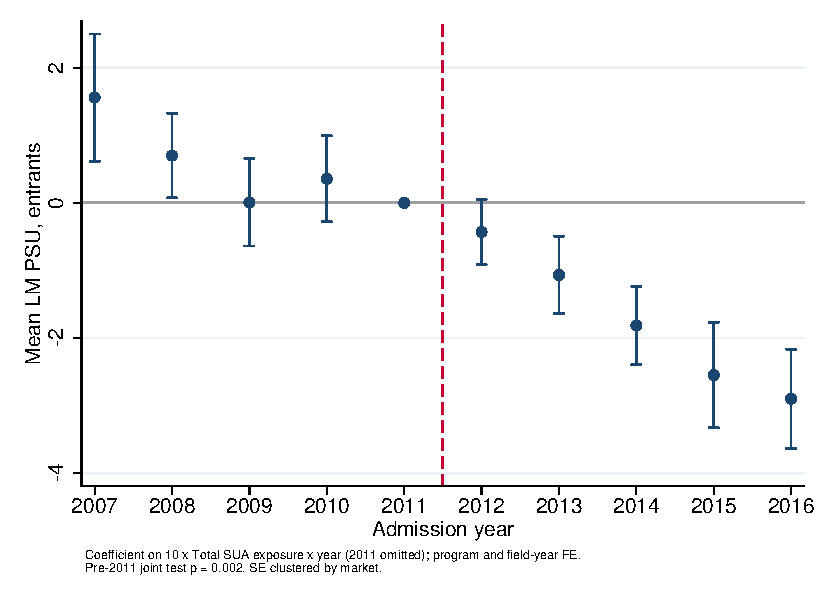
\includegraphics[width=\linewidth]{../../output/own_expansion/figures/oe_comp_sua_es_c_psu_mean.pdf}

\begin{itemize}\tiny
    \item With field $\times$ year FE, mean and last-admitted PSU fall in exposed incumbents.
    \item The decline starts \textbf{before} 2012 (pre-2011 joint test $p=0.002$), and it disappears with region $\times$ year FE.
    \item This mirrors the pre-trend problem of the SUA first stage: the result is not identified off 2012 entry.
\end{itemize}
\end{column}
\end{columns}
\end{frame}

%--------------------------------------------------------
\begin{frame}{Composition effects: Design IV (competitor vacancy shocks)}
\begin{columns}[T,onlytextwidth]
\begin{column}{0.56\textwidth}
\centering
\tiny
\resizebox{\linewidth}{!}{\begin{tabular}{lcccccc}
\toprule
 & \multicolumn{3}{c}{Field \(\times\) year FE} & \multicolumn{3}{c}{\(+\) Region \(\times\) year FE} \\
\cmidrule(lr){2-4}\cmidrule(lr){5-7}
Outcome & Total & Triangular & Gaussian & Total & Triangular & Gaussian \\
\midrule
First-year enrollment &   0.588 &   1.572 &   1.105 &   0.368 &   0.544 &   0.673 \\
 & ( 0.677) & ( 1.814) & ( 1.031) & ( 0.362) & ( 1.551) & ( 0.654) \\
\addlinespace
Mean LM PSU, entrants &  -0.535 &  -4.997\sym{*} &  -1.808 &  -0.008 &  -3.762\sym{**} &  -0.908 \\
 & ( 1.106) & ( 2.658) & ( 2.012) & ( 0.632) & ( 1.663) & ( 1.458) \\
LM PSU of the last admitted &  -1.787 &  -8.369\sym{**} &  -4.217\sym{*} &  -0.870 &  -5.664 &  -2.468 \\
 & ( 1.405) & ( 3.325) & ( 2.331) & ( 0.726) & ( 3.568) & ( 1.700) \\
SD of LM PSU, entrants &   0.395\sym{*} &   0.634 &   0.770\sym{*} &   0.168\sym{*} &  -0.034 &   0.380 \\
 & ( 0.213) & ( 1.128) & ( 0.434) & ( 0.101) & ( 0.743) & ( 0.259) \\
Mean NEM, entrants &  -0.726 &  -4.908 &  -2.017 &  -0.617 &  -5.784 &  -2.028 \\
 & ( 1.211) & ( 3.446) & ( 2.160) & ( 1.226) & ( 3.675) & ( 2.368) \\
Female, entrants, pct. &   0.146 &  -0.839 &   0.070 &   0.173 &  -0.508 &   0.198 \\
 & ( 0.227) & ( 0.719) & ( 0.500) & ( 0.186) & ( 0.752) & ( 0.445) \\
Private-paid school, entrants, pct. &   0.039 &   0.189 &   0.123 &   0.158\sym{*} &   0.585 &   0.370 \\
 & ( 0.153) & ( 0.556) & ( 0.292) & ( 0.090) & ( 0.588) & ( 0.248) \\
Municipal school, entrants, pct. &   0.688\sym{***} &  -0.313 &   0.835 &   0.622\sym{***} &  -0.099 &   0.831 \\
 & ( 0.246) & ( 1.717) & ( 0.773) & ( 0.173) & ( 1.282) & ( 0.596) \\
\midrule
Observations &  8,865 &  8,865 &  8,865 &  8,865 &  8,865 &  8,865 \\
\bottomrule
\end{tabular}
}

\vspace{0.05cm}
\parbox{\linewidth}{\tiny
\textit{Notes:} Design IV model (1), broad markets, exposure in 10 pp units, own-shock control, SE clustered by market.}
\end{column}
\begin{column}{0.42\textwidth}
\centering
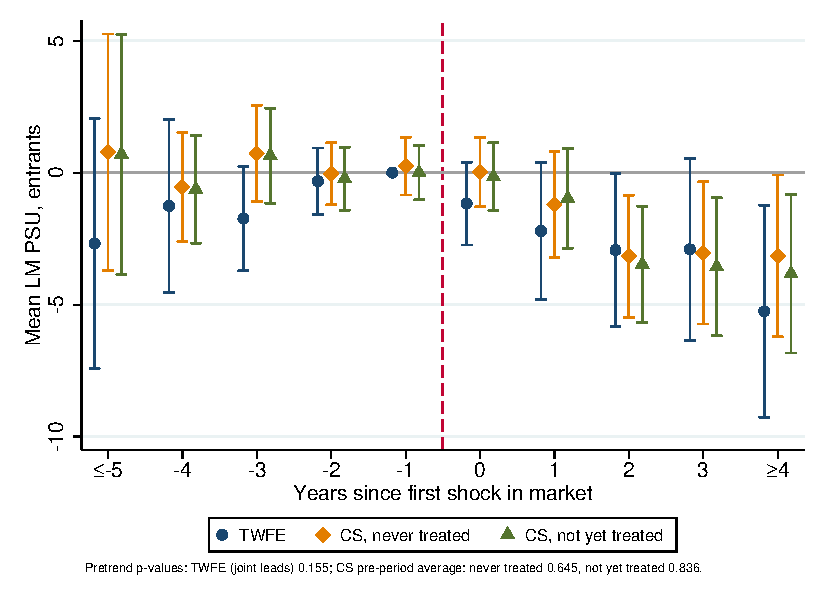
\includegraphics[width=\linewidth]{../../output/own_expansion/figures/oe_comp_vs_es_c_psu_mean.pdf}

\begin{itemize}\tiny
    \item Enrollment does not respond (as in Design IV). Under triangular weighting, mean entrant PSU falls by about 4--5 points per 10 pp.
    This is consistent with close-competitor expansions drawing away stronger applicants without changing the number of entrants.
    \item Total and Gaussian measures are mostly insignificant. The share from municipal schools rises by about 0.6--0.7 pp (Total).
\end{itemize}
\end{column}
\end{columns}
\end{frame}




\appendix
\section{Appendix}

\begin{frame}[label=nonharmonizedfields]{Non-harmonized field observations}

\begin{table}
\centering
\scriptsize
\begin{tabularx}{\textwidth}{lXccc}
\toprule
Institution & Program & Years & Code & Obs. \\
\midrule
UV & Bachillerato ingreso común & 2007--2008 & 1900 & 558 \\
USACH & Tecnólogo en alimentos (vesp) & 2007--2010 & 1690 & 208 \\
UV & Administración pública -- diurno & 2007 & 1997 & 26 \\
UV & Actuación teatral & 2008 & 1928 & 9 \\
\midrule
Total &  & 2007--2010 &  & 801 \\
\bottomrule
\end{tabularx}
\end{table}

\vskip 0.15cm

\footnotesize
These observations are excluded from the field-enriched sample because their program field could not be reliably harmonized. They represent 0.095\% of the baseline RDD sample within the main bandwidth.

\vskip 0.25cm

\hyperlink{descriptivestats}{\textcolor{blue}{\textsuperscript{$\leftarrow$ Back}}}

\end{frame}


%----------------------------------------------------
\begin{frame}[label=appendixretakesfield]{Appendix note 2: PSU retakes by field}

\centering
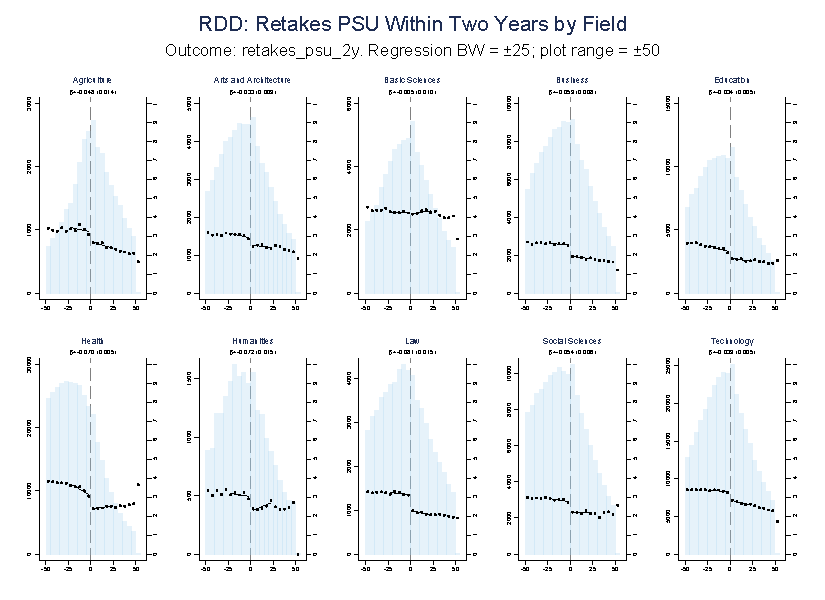
\includegraphics[width=0.92\textwidth]{../../output/figures/retakes_psu/rdd_retakes_psu_2y_by_field_combined.pdf}


\tiny
The reduction in PSU retaking is generally negative across fields, although magnitudes vary by academic area.\hyperlink{retakespsu}{\textcolor{blue}{\textsuperscript{$\leftarrow$ Back}}}

\end{frame}


%---------------------------------------------------------

%---------------------------------------------------------
\begin{frame}[label=sua-exposure-appendix]

\frametitle{
    SUA exposure: alternative field definitions
    \hfill
    \hyperlink{sua-exposure-main}{
        \scriptsize\color{blue}
        $\leftarrow$ Broad field
    }
}

\begin{columns}[T,onlytextwidth]

\begin{column}{0.495\textwidth}

\centering

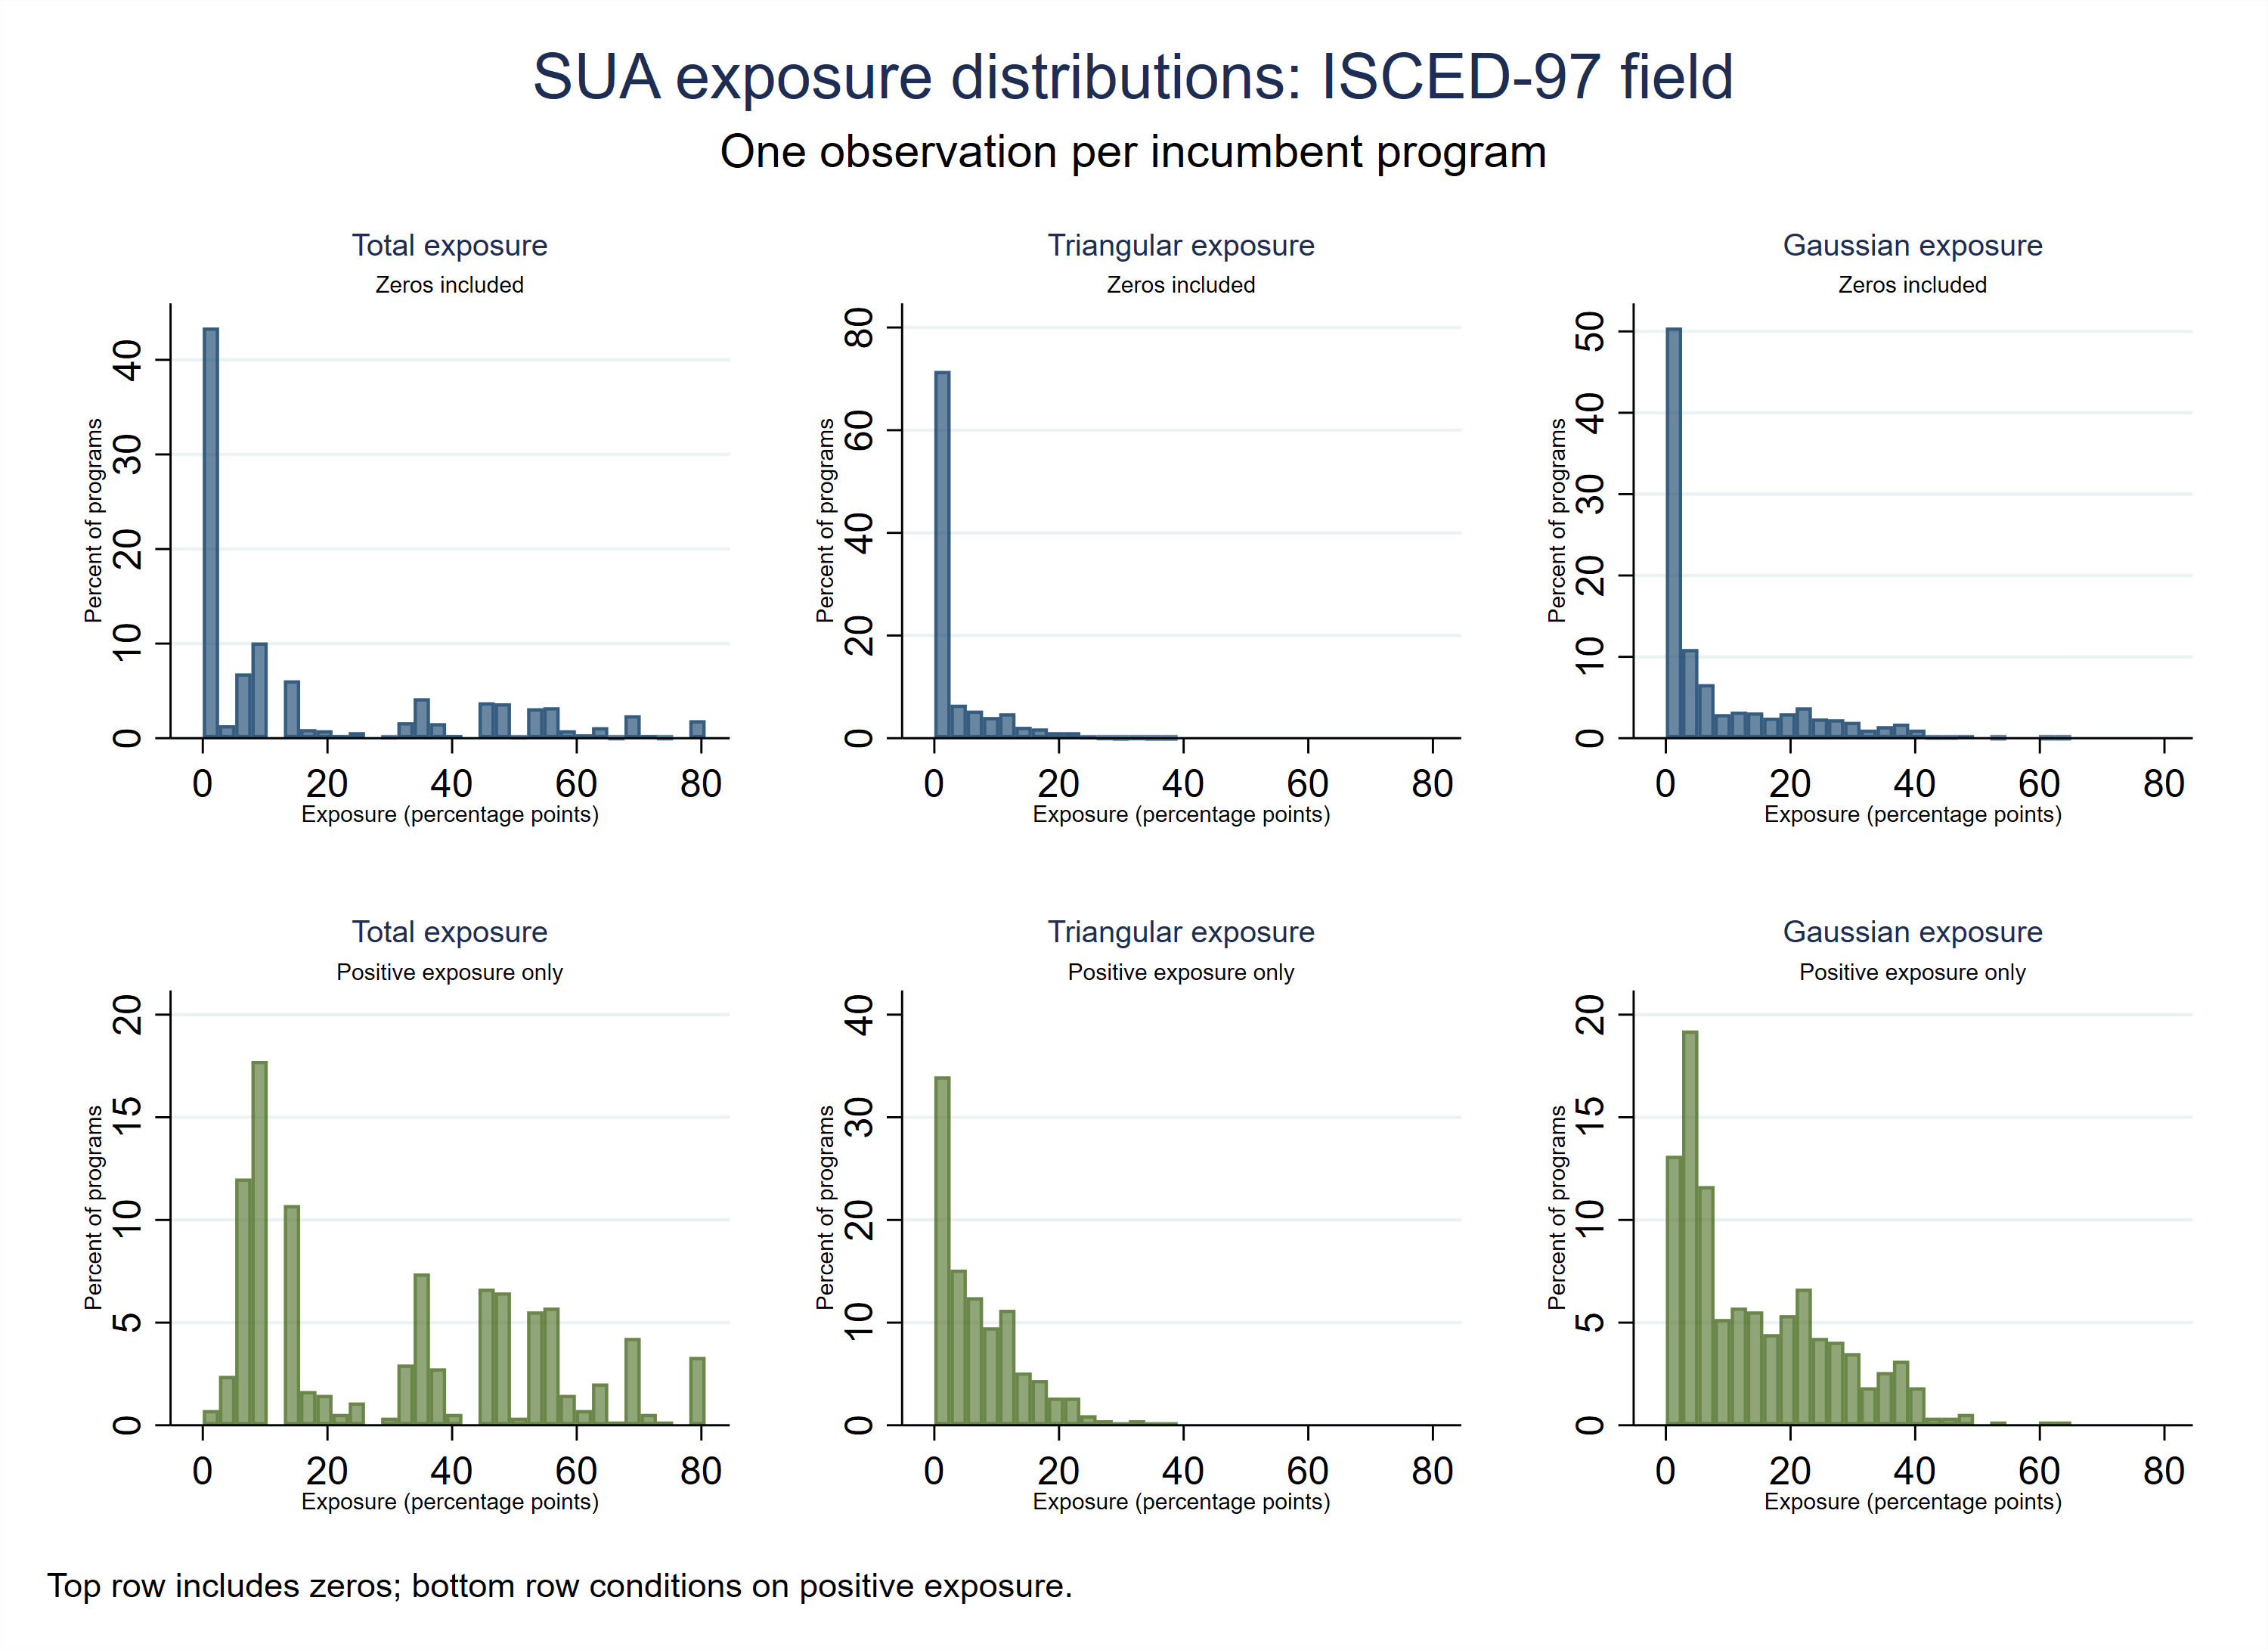
\includegraphics[ width=\linewidth, height=0.70\textheight, keepaspectratio ]{../../output/sua_exposure_distributions_isced.png}

\end{column}

\begin{column}{0.495\textwidth}

\centering

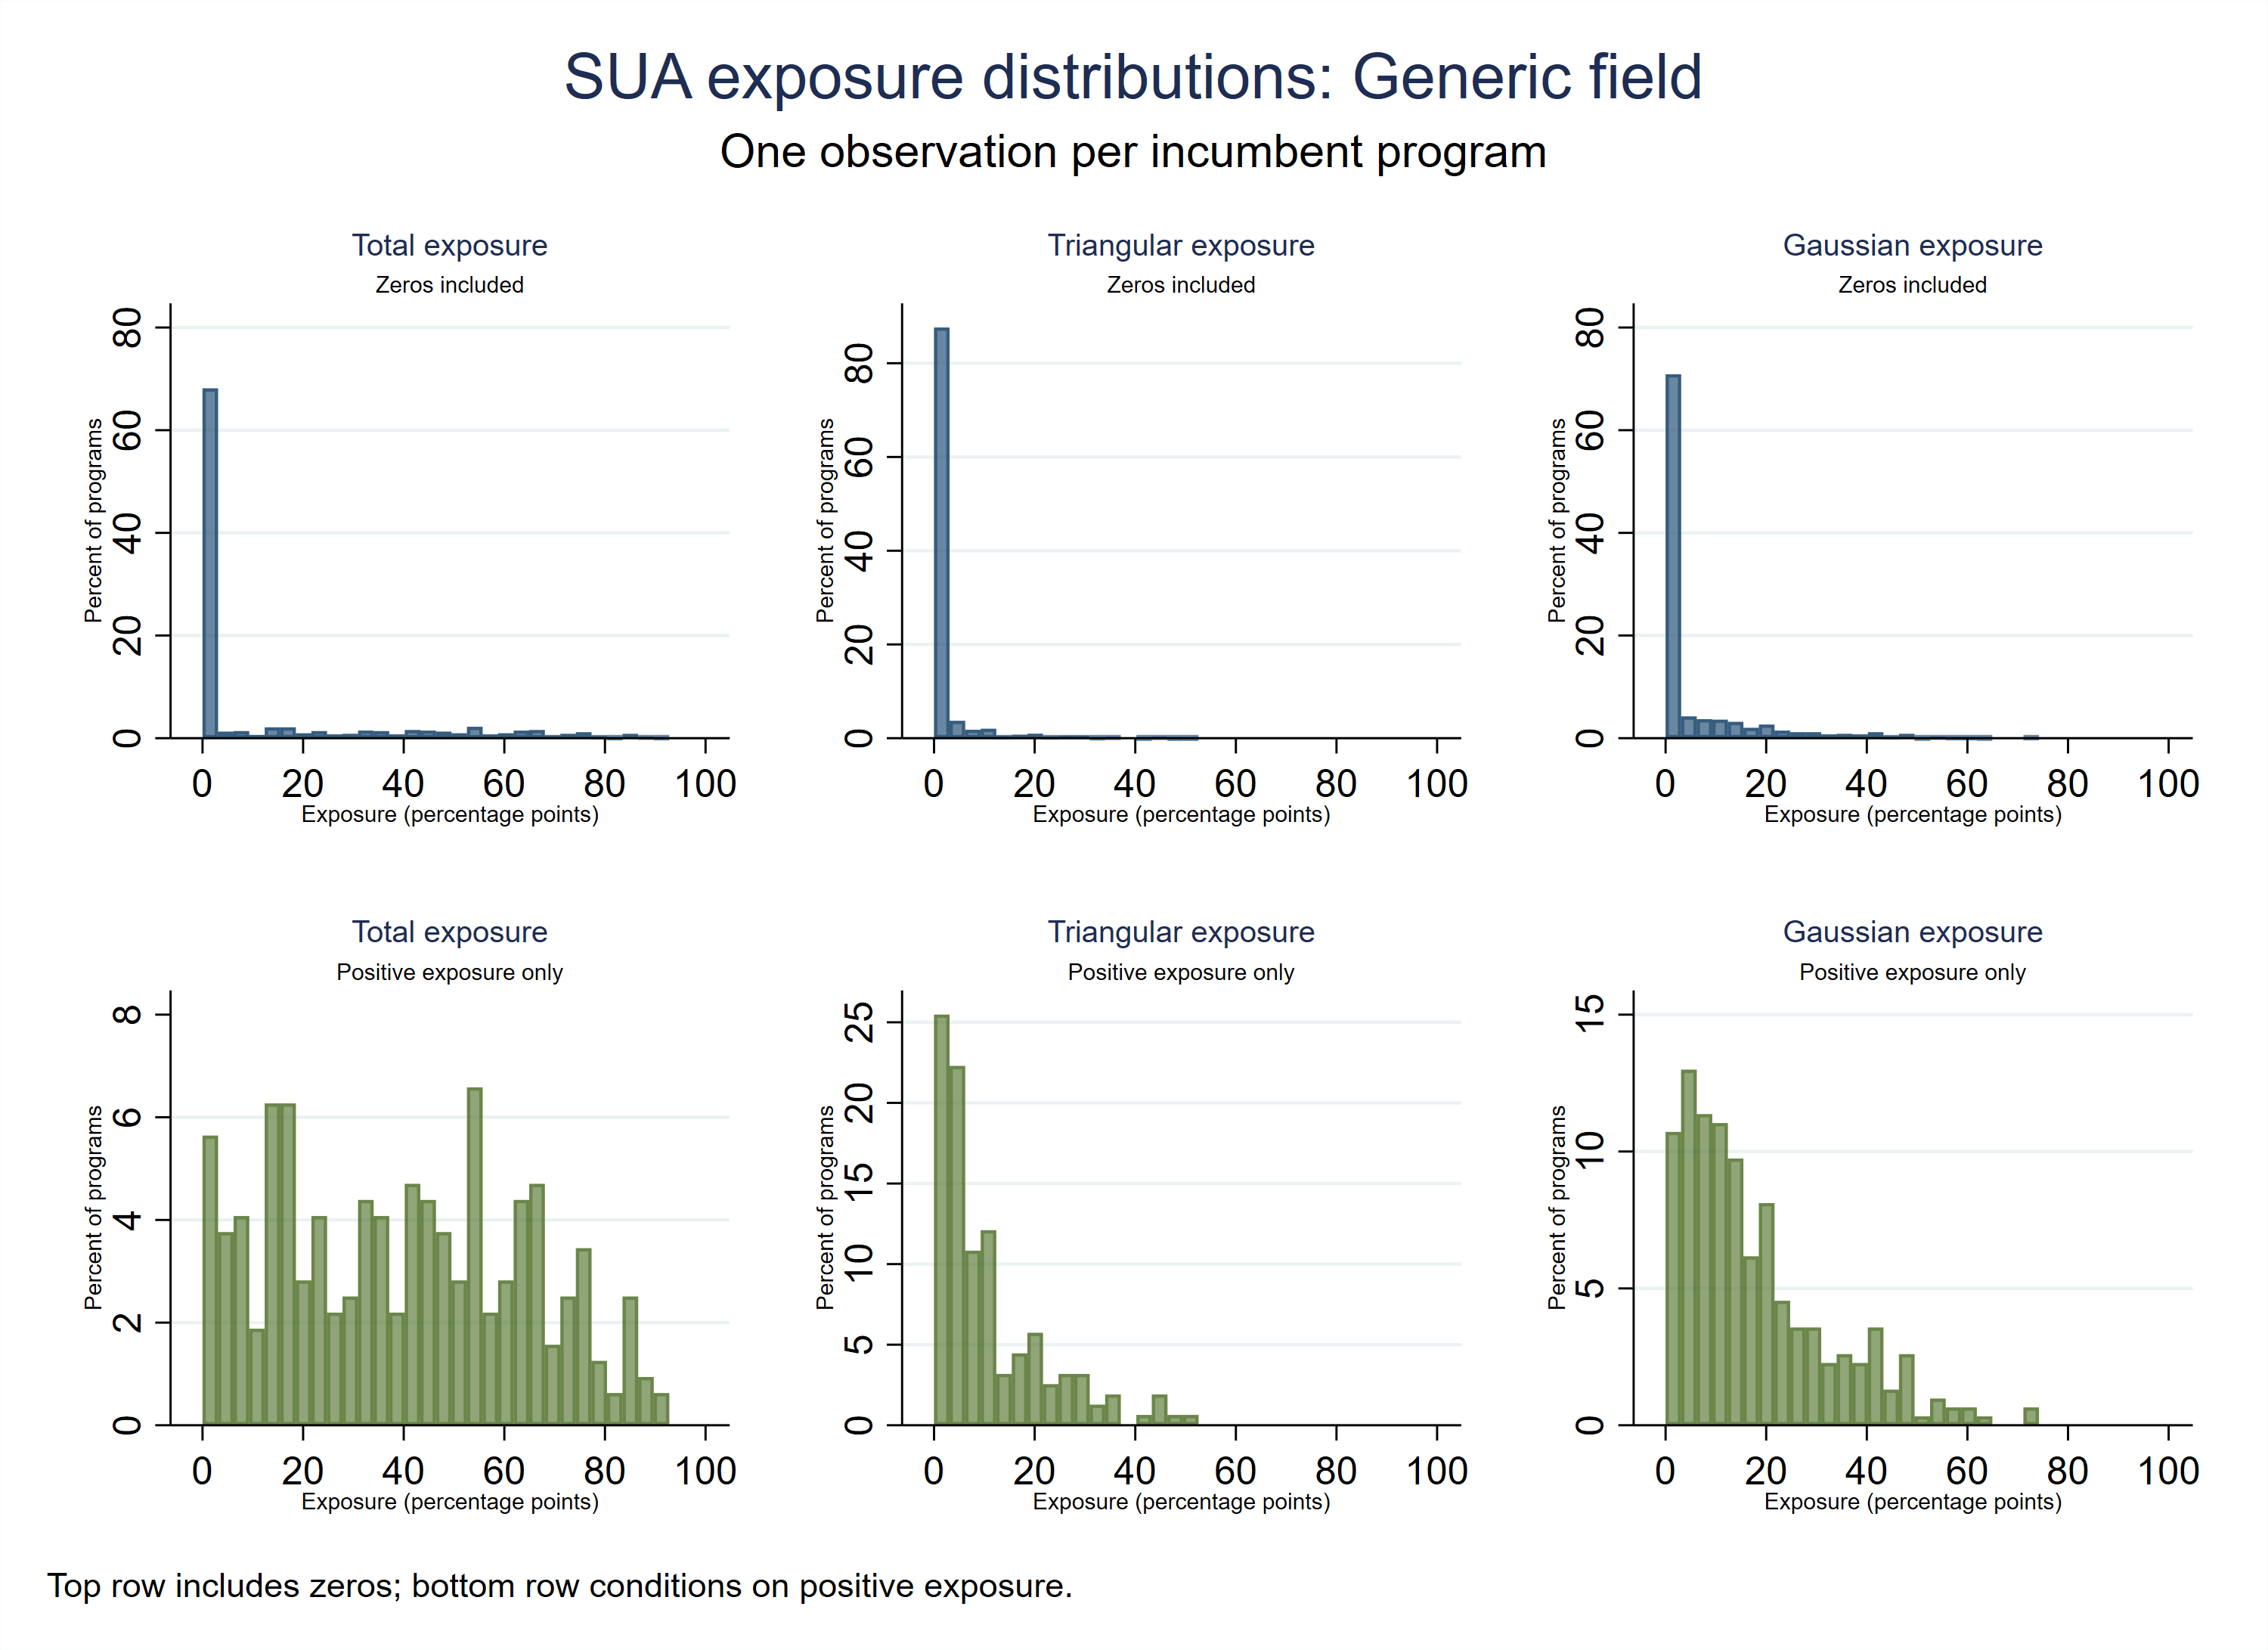
\includegraphics[ width=\linewidth, height=0.70\textheight, keepaspectratio ]{../../output/sua_exposure_distributions_generic.png}

\end{column}

\end{columns}

\vspace{0.02cm}

\centering
\tiny
Narrower field definitions generate more markets and a larger share of
zero-exposure programs, particularly under the Generic-field definition.

\end{frame}

%---------------------------------------------------------
\begin{frame}[label=sua-fs-lvl-entrant]

\frametitle{
    First stage: regions with entrant universities only
    \hfill
    \hyperlink{sua-first-stage}{\scriptsize\color{blue}$\leftarrow$ Main}
    \hyperlink{sua-es-lvl-entrant}{\scriptsize\color{blue}ES $\rightarrow$}
}

\centering

\vspace{-0.2cm}

{\small
\begin{equation*}
N^{\mathrm{first}}_{pt}
=
\pi
\left(
E^{k,m}_{p}\times Post_t
\right)
+\mu_p
+\alpha_{f_m(p),t}
+\gamma_{r(p),t}
+\nu_{pt}.
\end{equation*}
}

\vspace{-0.3cm}

\resizebox{0.62\textwidth}{!}{\begin{tabular}{lcccccc}
\toprule
 & \multicolumn{3}{c}{Field \(\times\) year FE} & \multicolumn{3}{c}{\(+\) Region \(\times\) year FE} \\
\cmidrule(lr){2-4}\cmidrule(lr){5-7}
Exposure measure & Broad & ISCED-97 & Generic & Broad & ISCED-97 & Generic \\
\midrule
\textit{Total} &  2.807\sym{***} &  2.609\sym{***} &  2.378\sym{***} & -0.492 &  0.652 &  0.151 \\
 & (0.457) & (0.415) & (0.381) & (0.940) & (0.573) & (0.504) \\
\quad Wald \(F\) & 37.81 & 39.49 & 38.90 &  0.27 &  1.30 &  0.09 \\
\quad Programs with zero exposure &        10 &        60 &       256 &        10 &        60 &       256 \\
\addlinespace
\textit{Triangular} & -2.133 & -0.830 &  0.711 & -6.390\sym{**} & -4.179\sym{***} & -1.575 \\
 & (1.482) & (1.253) & (1.071) & (2.434) & (1.581) & (1.033) \\
\quad Wald \(F\) &  2.07 &  0.44 &  0.44 &  6.89 &  6.99 &  2.33 \\
\quad Programs with zero exposure &        96 &       192 &       416 &        96 &       192 &       416 \\
\addlinespace
\textit{Gaussian} &  0.545 &  1.118 &  1.652\sym{**} & -4.168\sym{**} & -2.416\sym{**} & -1.240 \\
 & (0.892) & (0.764) & (0.725) & (1.863) & (1.177) & (0.773) \\
\quad Wald \(F\) &  0.37 &  2.14 &  5.19 &  5.01 &  4.21 &  2.58 \\
\quad Programs with zero exposure &        10 &        60 &       267 &        10 &        60 &       267 \\
\midrule
Observations &     5,090 &     5,080 &     4,781 &     5,090 &     5,080 &     4,781 \\
Programs &       601 &       601 &       571 &       601 &       601 &       571 \\
Markets &        40 &        80 &       303 &        40 &        80 &       303 \\
Regions &         4 &         4 &         4 &         4 &         4 &         4 \\
Program FE & Yes & Yes & Yes & Yes & Yes & Yes \\
Field \(\times\) year FE & Yes & Yes & Yes & Yes & Yes & Yes \\
Region \(\times\) year FE & No & No & No & Yes & Yes & Yes \\
\bottomrule
\end{tabular}
}

\vspace{0.05cm}

\parbox{0.97\textwidth}{%
\tiny
\textit{Notes:}
Sample restricted to incumbent programs in the four pre-treatment regions with entrant programs in 2009--2011 (Valpara\'iso, Biob\'io, La Araucan\'ia, Metropolitana); outside them exposure is zero by construction.
Same specification as the main first stage. Exposure in 10 percentage-point units; SE clustered by pre-treatment market.
$^{***}p<0.01$, $^{**}p<0.05$, $^{*}p<0.10$.
}

\end{frame}

%---------------------------------------------------------
\begin{frame}[label=sua-es-lvl-entrant]

\frametitle{
    Event studies: regions with entrant universities only
    \hfill
    \hyperlink{sua-fs-lvl-entrant}{\scriptsize\color{blue}$\leftarrow$ First stage}
}

\vspace{-0.12cm}

\begin{columns}[T,onlytextwidth]
    \begin{column}{0.495\textwidth}
        \centering
        \textbf{\scriptsize Field $\times$ year FE}

        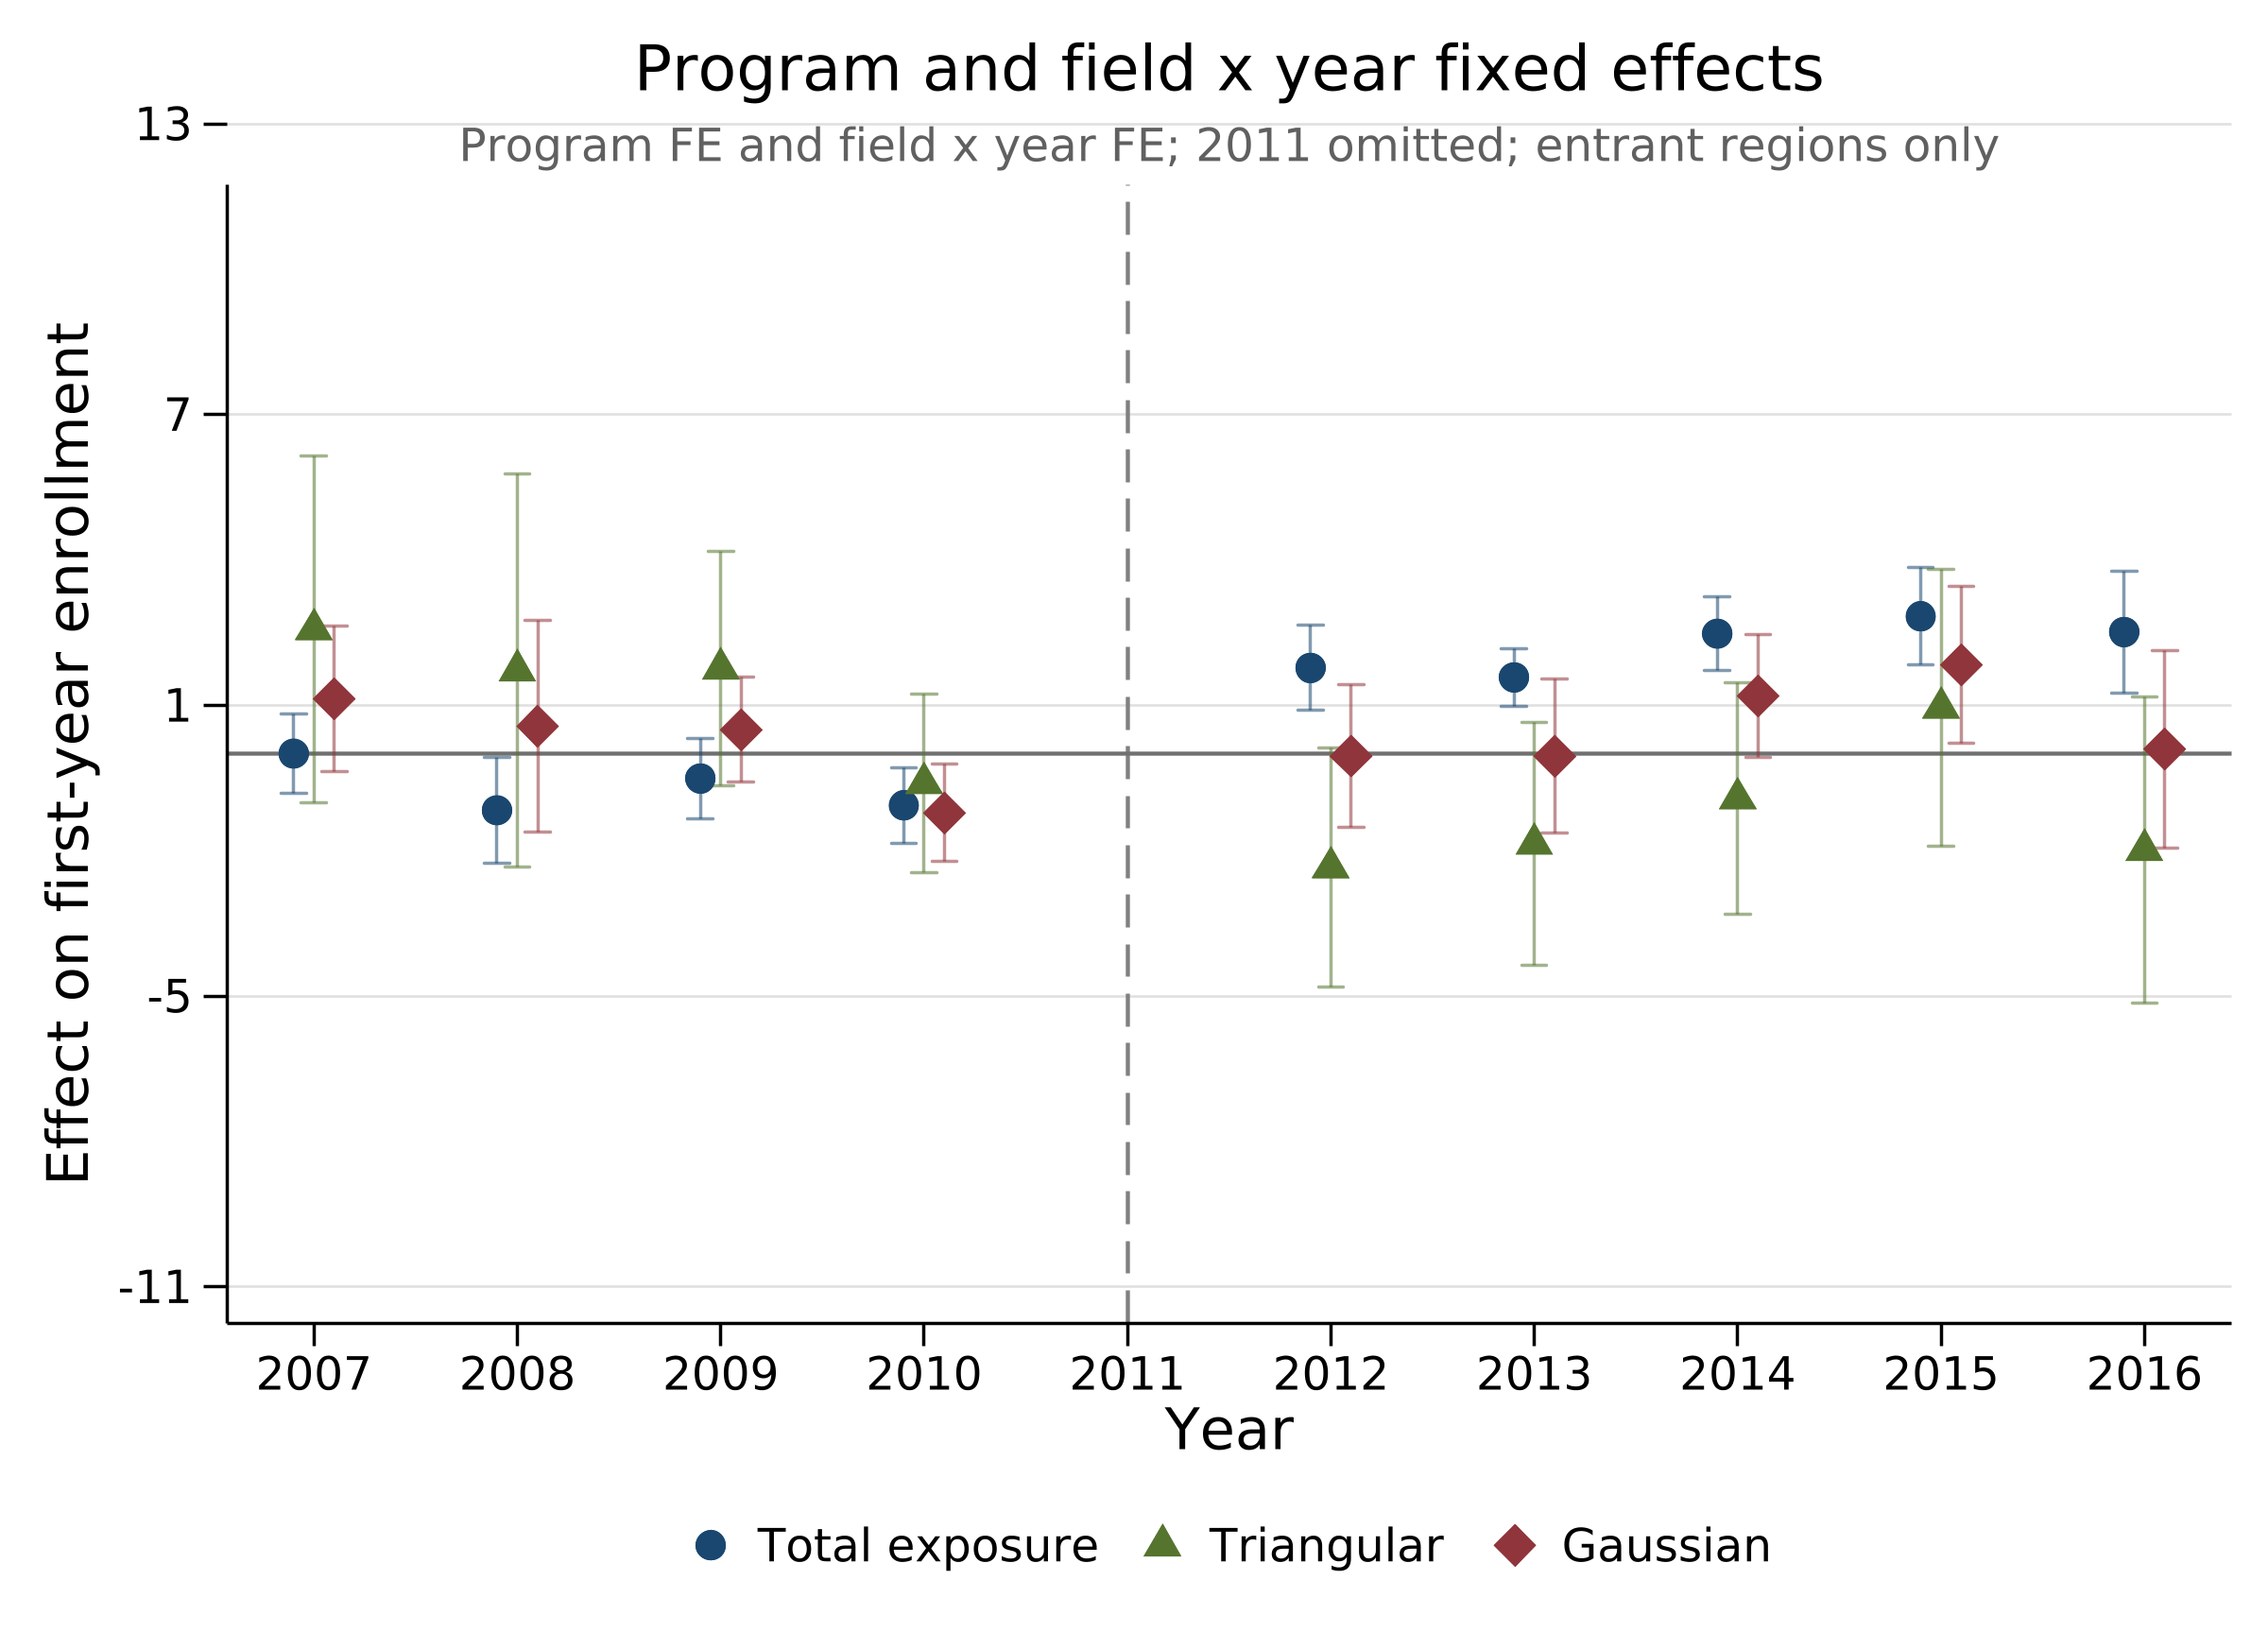
\includegraphics[width=\linewidth, height=0.66\textheight, keepaspectratio]{../../output/sua_event_study_exposure_comparison_baseline_entrant.png}
    \end{column}
    \begin{column}{0.495\textwidth}
        \centering
        \textbf{\scriptsize $+$ Region $\times$ year FE}

        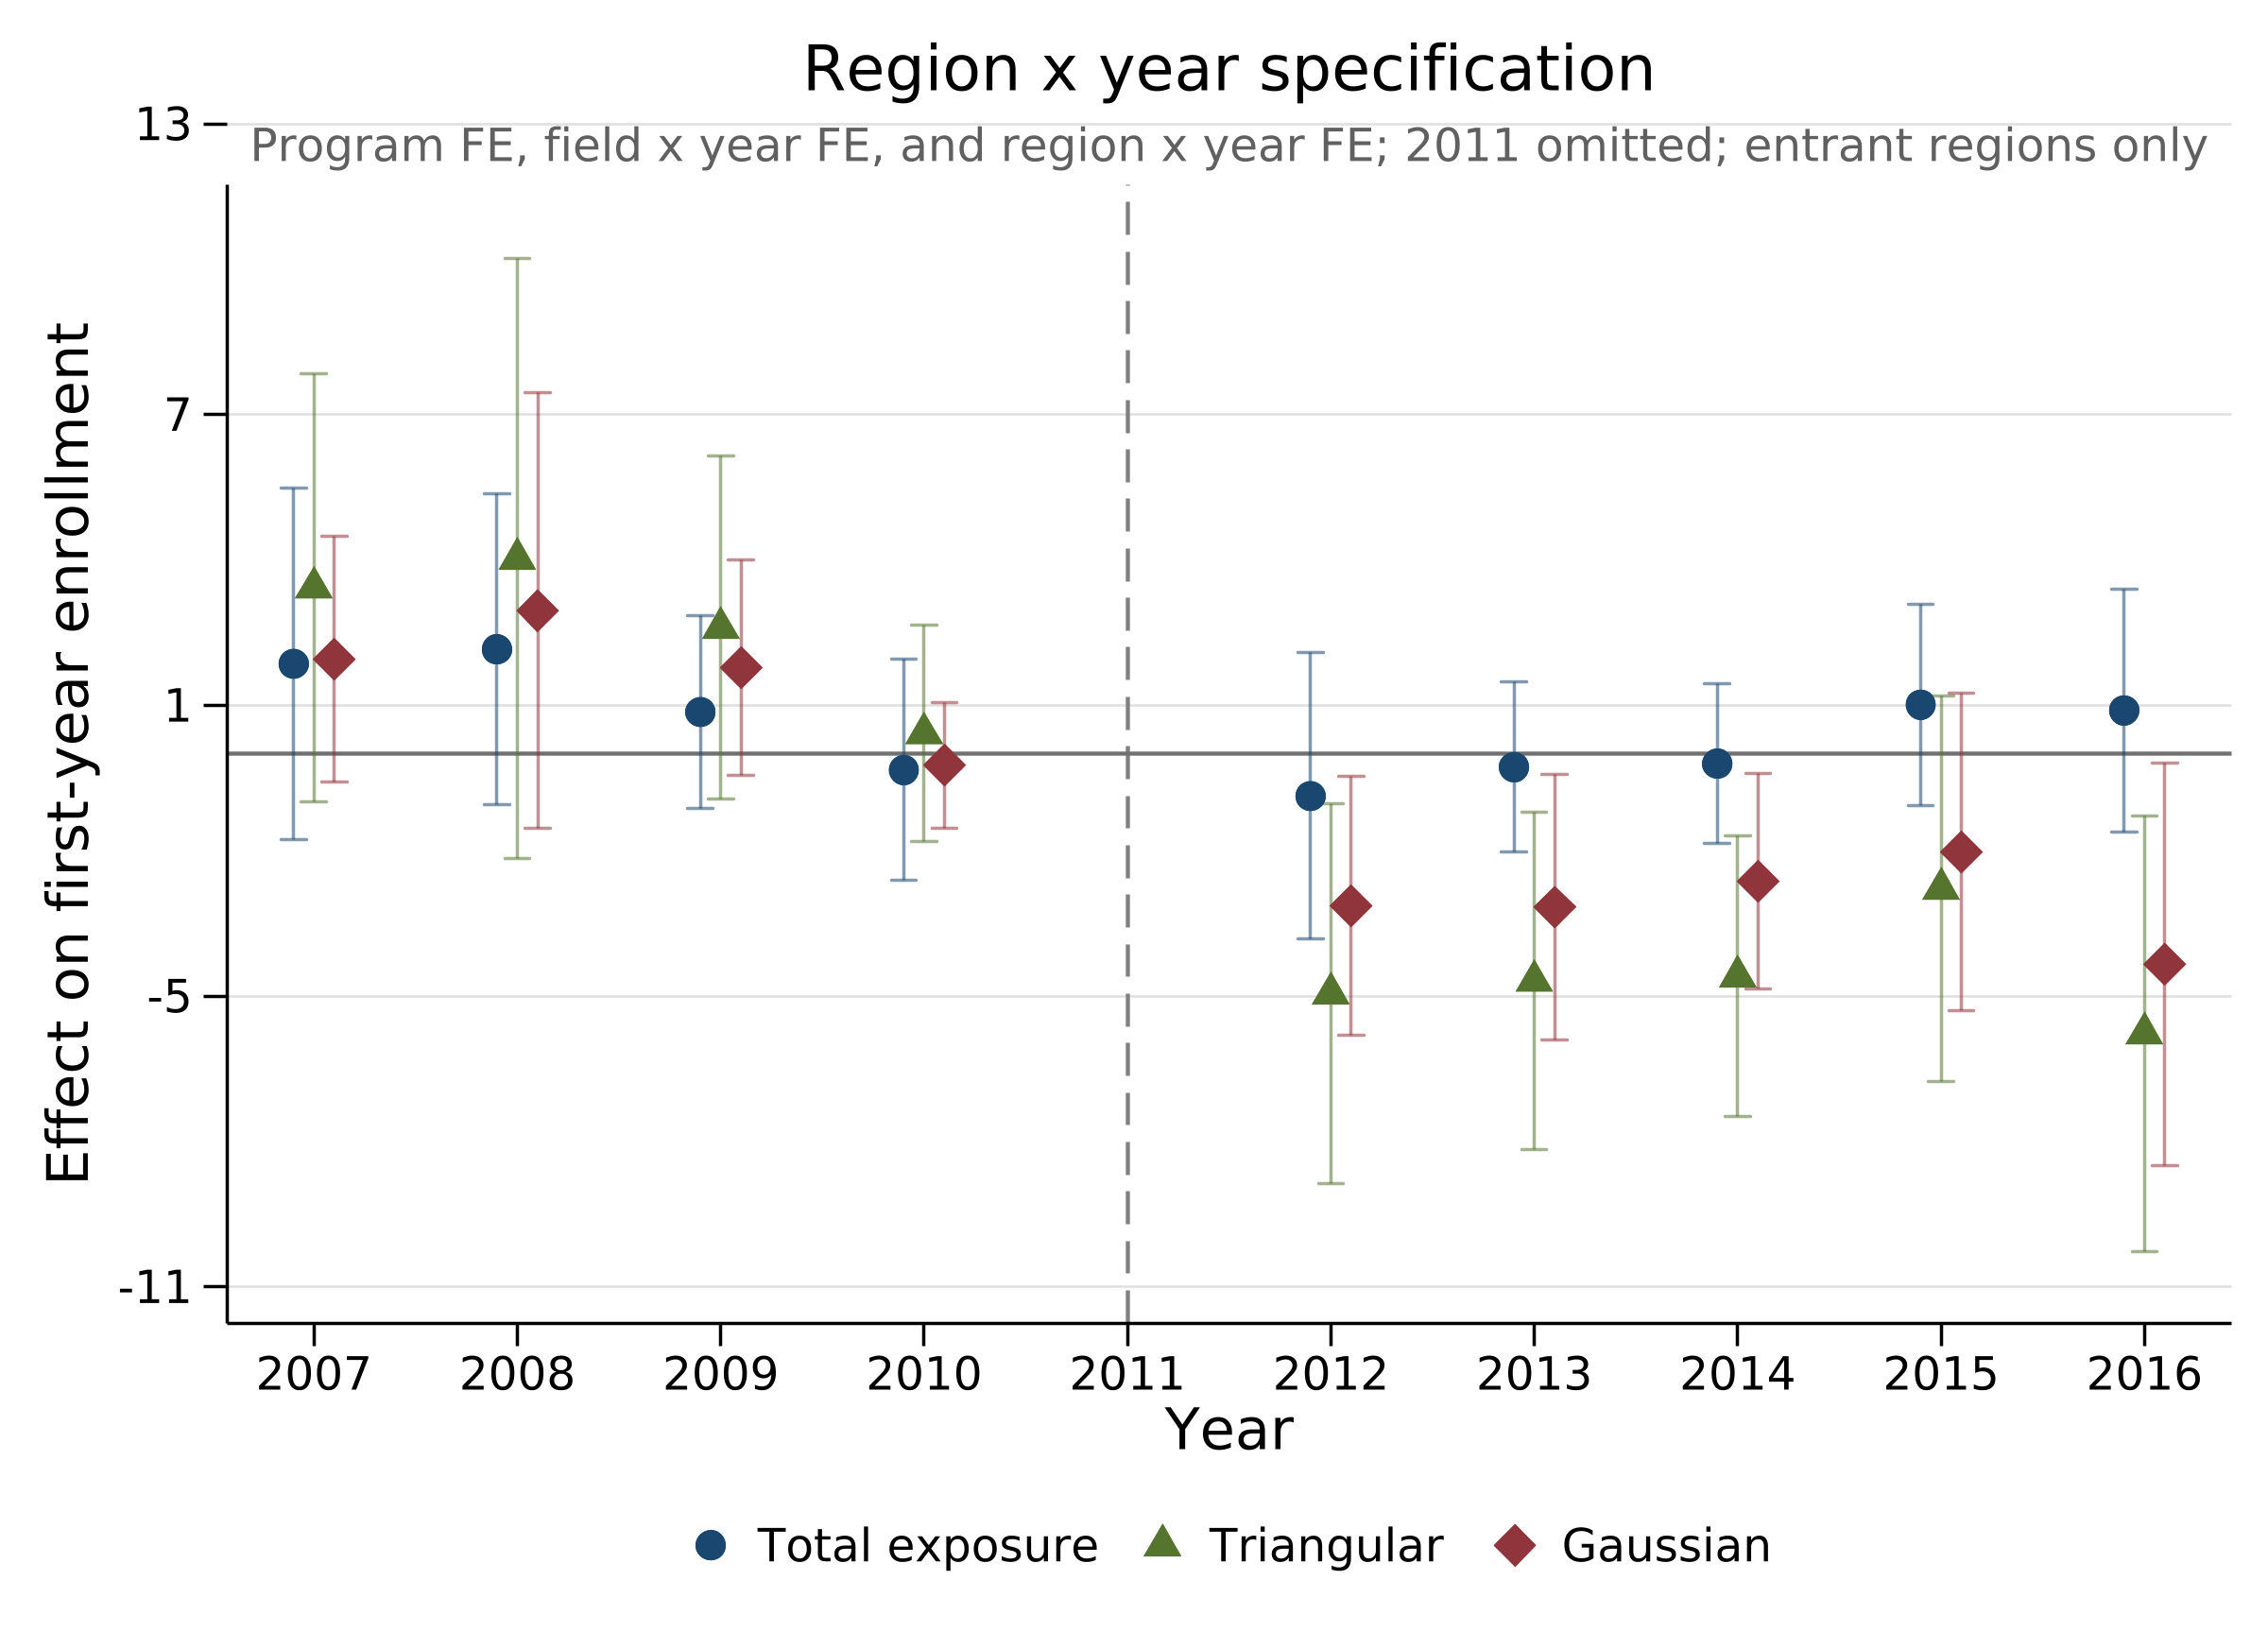
\includegraphics[width=\linewidth, height=0.66\textheight, keepaspectratio]{../../output/sua_event_study_exposure_comparison_regionyear_entrant.png}
    \end{column}
\end{columns}

\vspace{0.04cm}

\begin{center}
\begin{minipage}{0.96\textwidth}
\tiny
\textit{Notes:}
Sample restricted to incumbent programs in the four pre-treatment regions with entrant programs in 2009--2011 (Valpara\'iso, Biob\'io, La Araucan\'ia, Metropolitana); outside them exposure is zero by construction.
Broad-field markets; separate event studies for Total, Triangular and Gaussian
exposure. Coefficients measure the enrollment difference associated with a 10 percentage-point increase in exposure in each year relative to 2011. 95\% confidence intervals; SE clustered by pre-treatment market.
Joint pretrend $p$-values (2007--2010) for Total, Triangular and Gaussian are
0.046, 0.068 and 0.010 in the left panel, and 0.151, 0.302 and 0.209 in the right panel.
\end{minipage}
\end{center}

\end{frame}

%---------------------------------------------------------
\begin{frame}[label=sua-fs-lvl-positive]

\frametitle{
    First stage: positive exposure only
    \hfill
    \hyperlink{sua-first-stage}{\scriptsize\color{blue}$\leftarrow$ Main}
    \hyperlink{sua-es-lvl-positive}{\scriptsize\color{blue}ES $\rightarrow$}
}

\centering

\vspace{-0.2cm}

{\small
\begin{equation*}
N^{\mathrm{first}}_{pt}
=
\pi
\left(
E^{k,m}_{p}\times Post_t
\right)
+\mu_p
+\alpha_{f_m(p),t}
+\gamma_{r(p),t}
+\nu_{pt}.
\end{equation*}
}

\vspace{-0.3cm}

\resizebox{0.62\textwidth}{!}{\begin{tabular}{lcccccc}
\toprule
 & \multicolumn{3}{c}{Field \(\times\) year FE} & \multicolumn{3}{c}{\(+\) Region \(\times\) year FE} \\
\cmidrule(lr){2-4}\cmidrule(lr){5-7}
Exposure measure & Broad & ISCED-97 & Generic & Broad & ISCED-97 & Generic \\
\midrule
\textit{Total} &  2.753\sym{***} &  2.423\sym{***} &  2.579\sym{***} & -0.863 &  1.086 & -1.266 \\
 & (0.474) & (0.443) & (0.575) & (0.952) & (0.911) & (1.144) \\
\quad Wald \(F\) & 33.68 & 29.84 & 20.11 &  0.82 &  1.42 &  1.23 \\
\quad Programs &       591 &       540 &       304 &       591 &       540 &       304 \\
\addlinespace
\textit{Triangular} & -0.668 &  0.555 &  0.385 & -4.698\sym{**} & -2.671 & -1.705 \\
 & (1.454) & (1.264) & (1.496) & (2.119) & (1.678) & (1.624) \\
\quad Wald \(F\) &  0.21 &  0.19 &  0.07 &  4.91 &  2.54 &  1.10 \\
\quad Programs &       505 &       407 &       142 &       505 &       407 &       142 \\
\addlinespace
\textit{Gaussian} &  0.378 &  0.805 &  0.489 & -4.196\sym{**} & -2.576\sym{*} & -2.133\sym{**} \\
 & (0.908) & (0.798) & (0.874) & (1.865) & (1.289) & (0.897) \\
\quad Wald \(F\) &  0.17 &  1.02 &  0.31 &  5.06 &  4.00 &  5.65 \\
\quad Programs &       591 &       540 &       292 &       591 &       540 &       292 \\
\midrule
Observations (Total) &     5,009 &     4,571 &     2,516 &     5,009 &     4,571 &     2,516 \\
Programs (Total) &       591 &       540 &       304 &       591 &       540 &       304 \\
Markets (Total) &        36 &        59 &       131 &        36 &        59 &       131 \\
Regions &         4 &         4 &         4 &         4 &         4 &         4 \\
Program FE & Yes & Yes & Yes & Yes & Yes & Yes \\
Field \(\times\) year FE & Yes & Yes & Yes & Yes & Yes & Yes \\
Region \(\times\) year FE & No & No & No & Yes & Yes & Yes \\
\bottomrule
\end{tabular}
}

\vspace{0.05cm}

\parbox{0.97\textwidth}{%
\tiny
\textit{Notes:}
Sample restricted to programs with positive exposure, defined separately for each measure (Triangular exposure can be zero where Total and Gaussian are positive). All such programs lie in the four regions with entrant programs, so the only difference with the entrant-region sample is that zero-exposure programs within those regions are dropped.
Same specification as the main first stage. Exposure in 10 percentage-point units; SE clustered by pre-treatment market.
$^{***}p<0.01$, $^{**}p<0.05$, $^{*}p<0.10$.
}

\end{frame}

%---------------------------------------------------------
\begin{frame}[label=sua-es-lvl-positive]

\frametitle{
    Event studies: positive exposure only
    \hfill
    \hyperlink{sua-fs-lvl-positive}{\scriptsize\color{blue}$\leftarrow$ First stage}
}

\vspace{-0.12cm}

\begin{columns}[T,onlytextwidth]
    \begin{column}{0.495\textwidth}
        \centering
        \textbf{\scriptsize Field $\times$ year FE}

        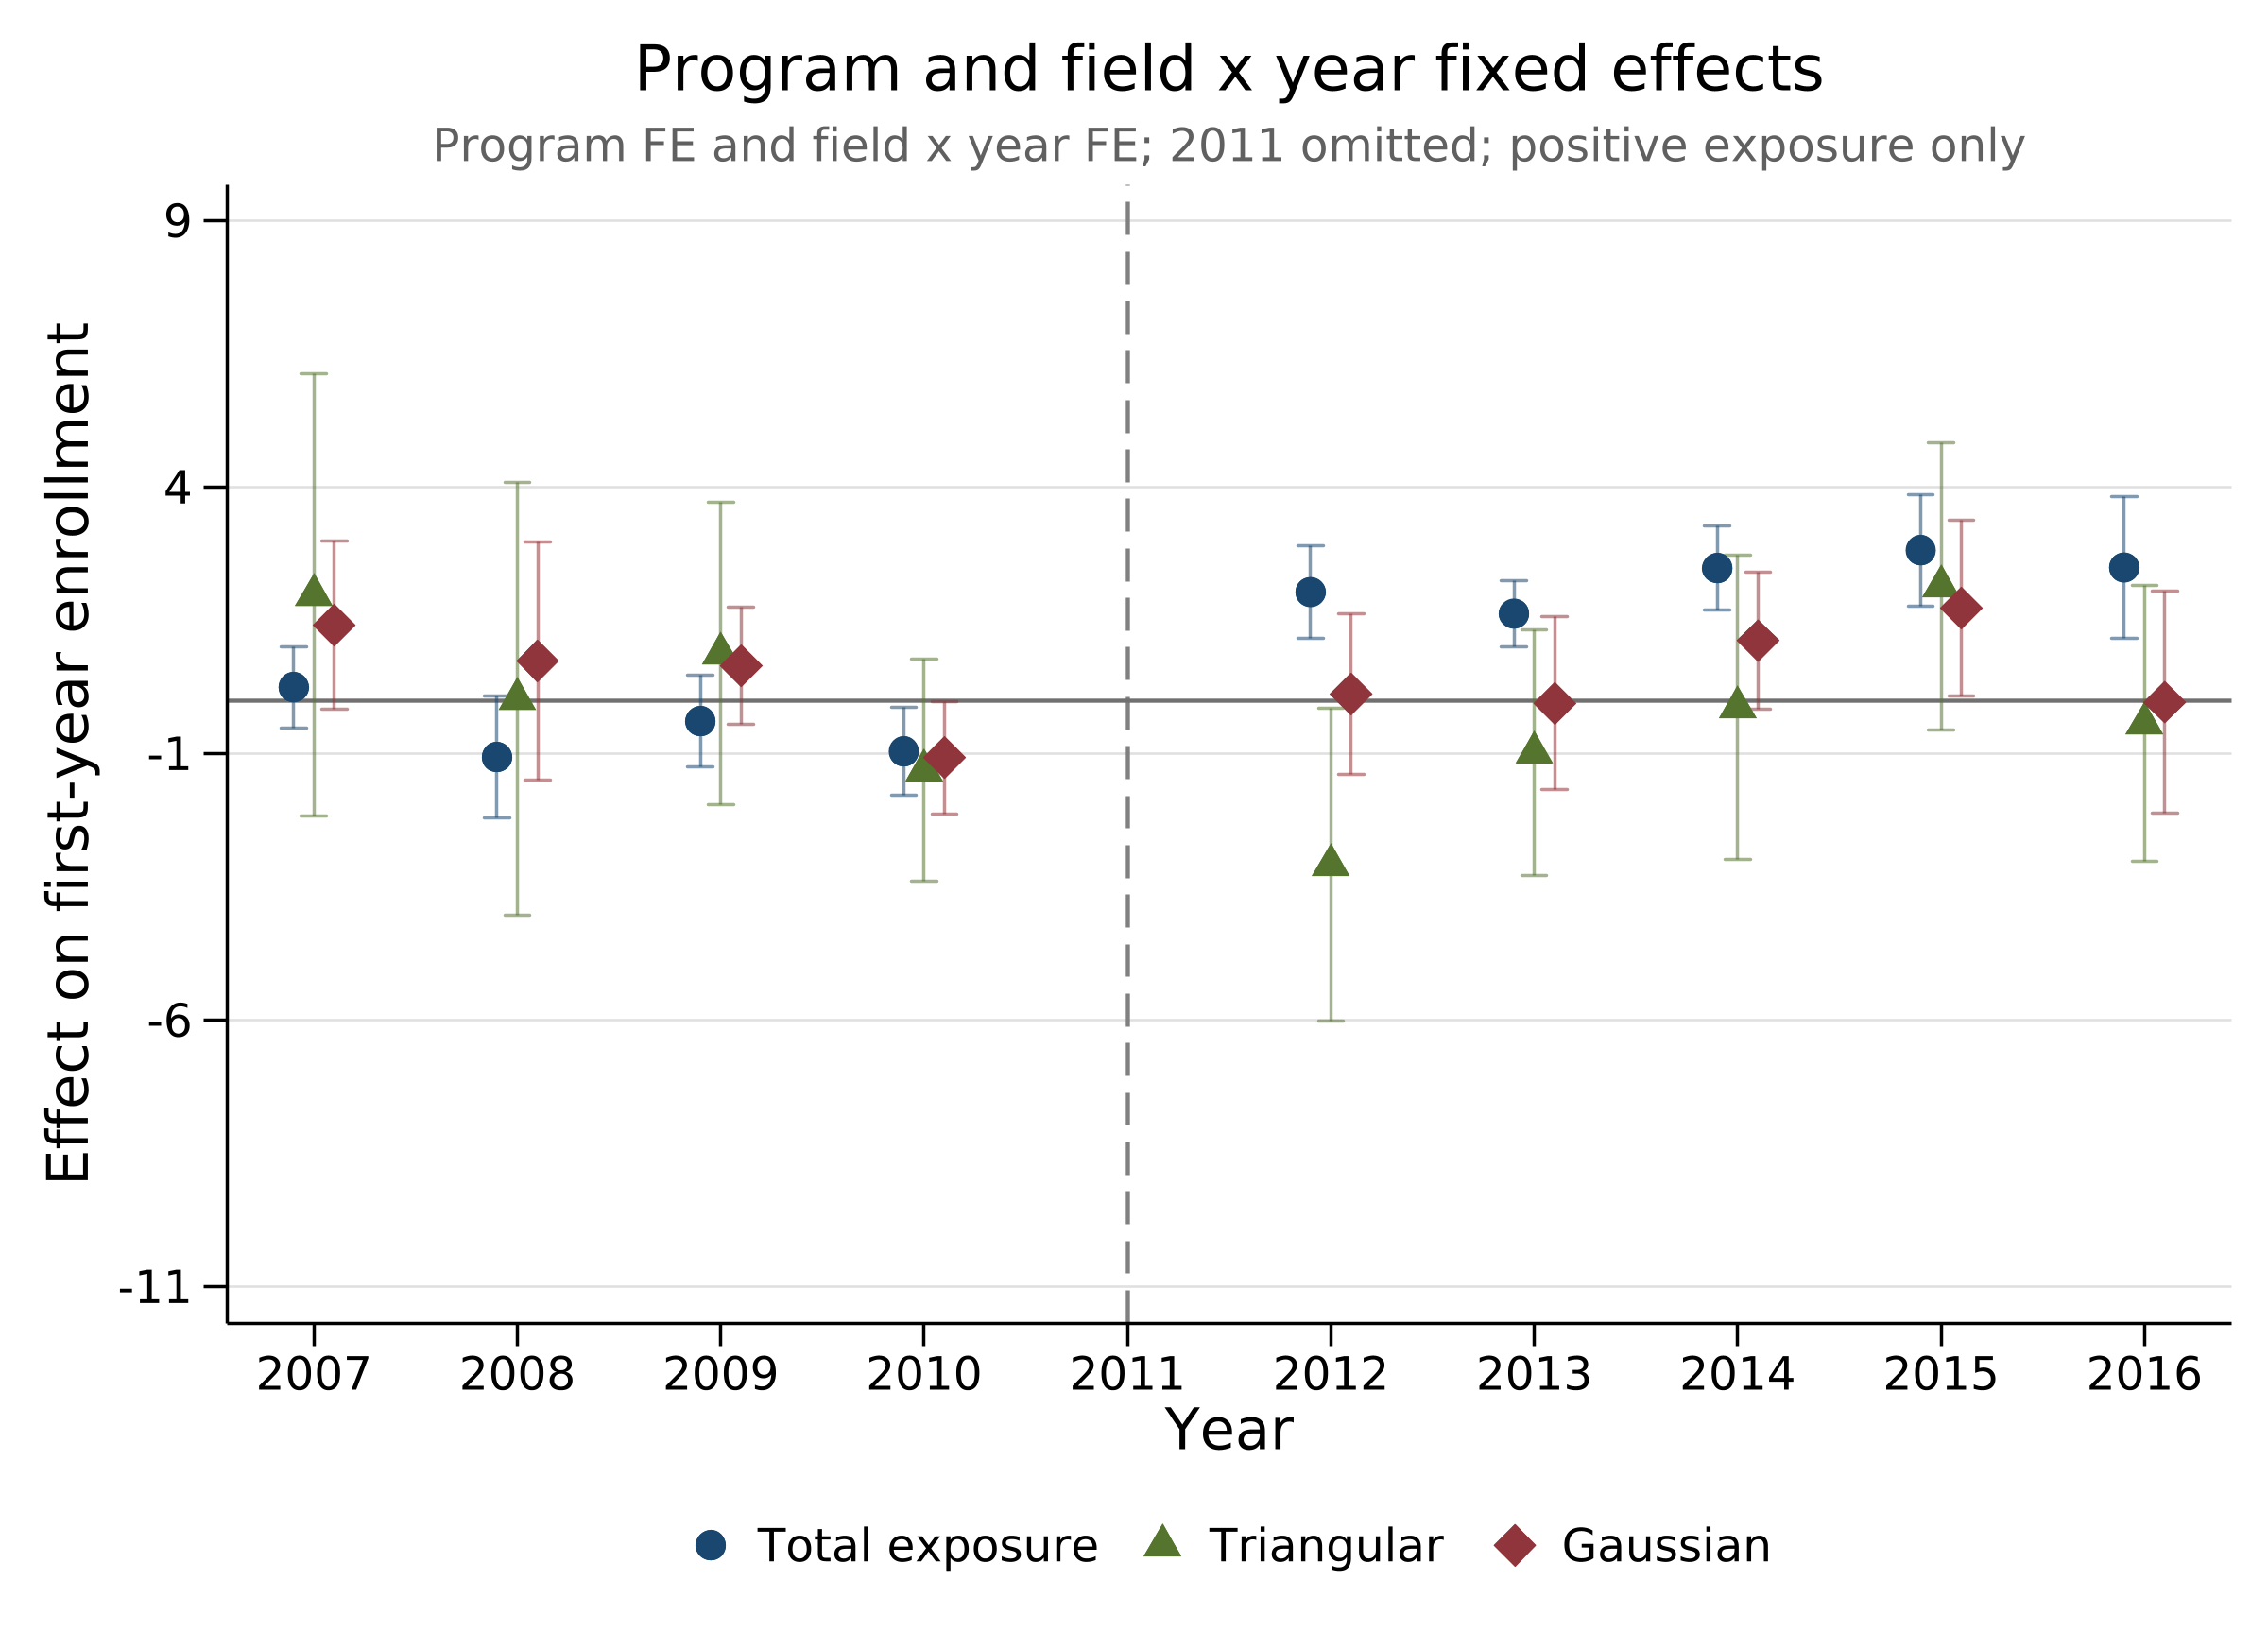
\includegraphics[width=\linewidth, height=0.66\textheight, keepaspectratio]{../../output/sua_event_study_exposure_comparison_baseline_positive.png}
    \end{column}
    \begin{column}{0.495\textwidth}
        \centering
        \textbf{\scriptsize $+$ Region $\times$ year FE}

        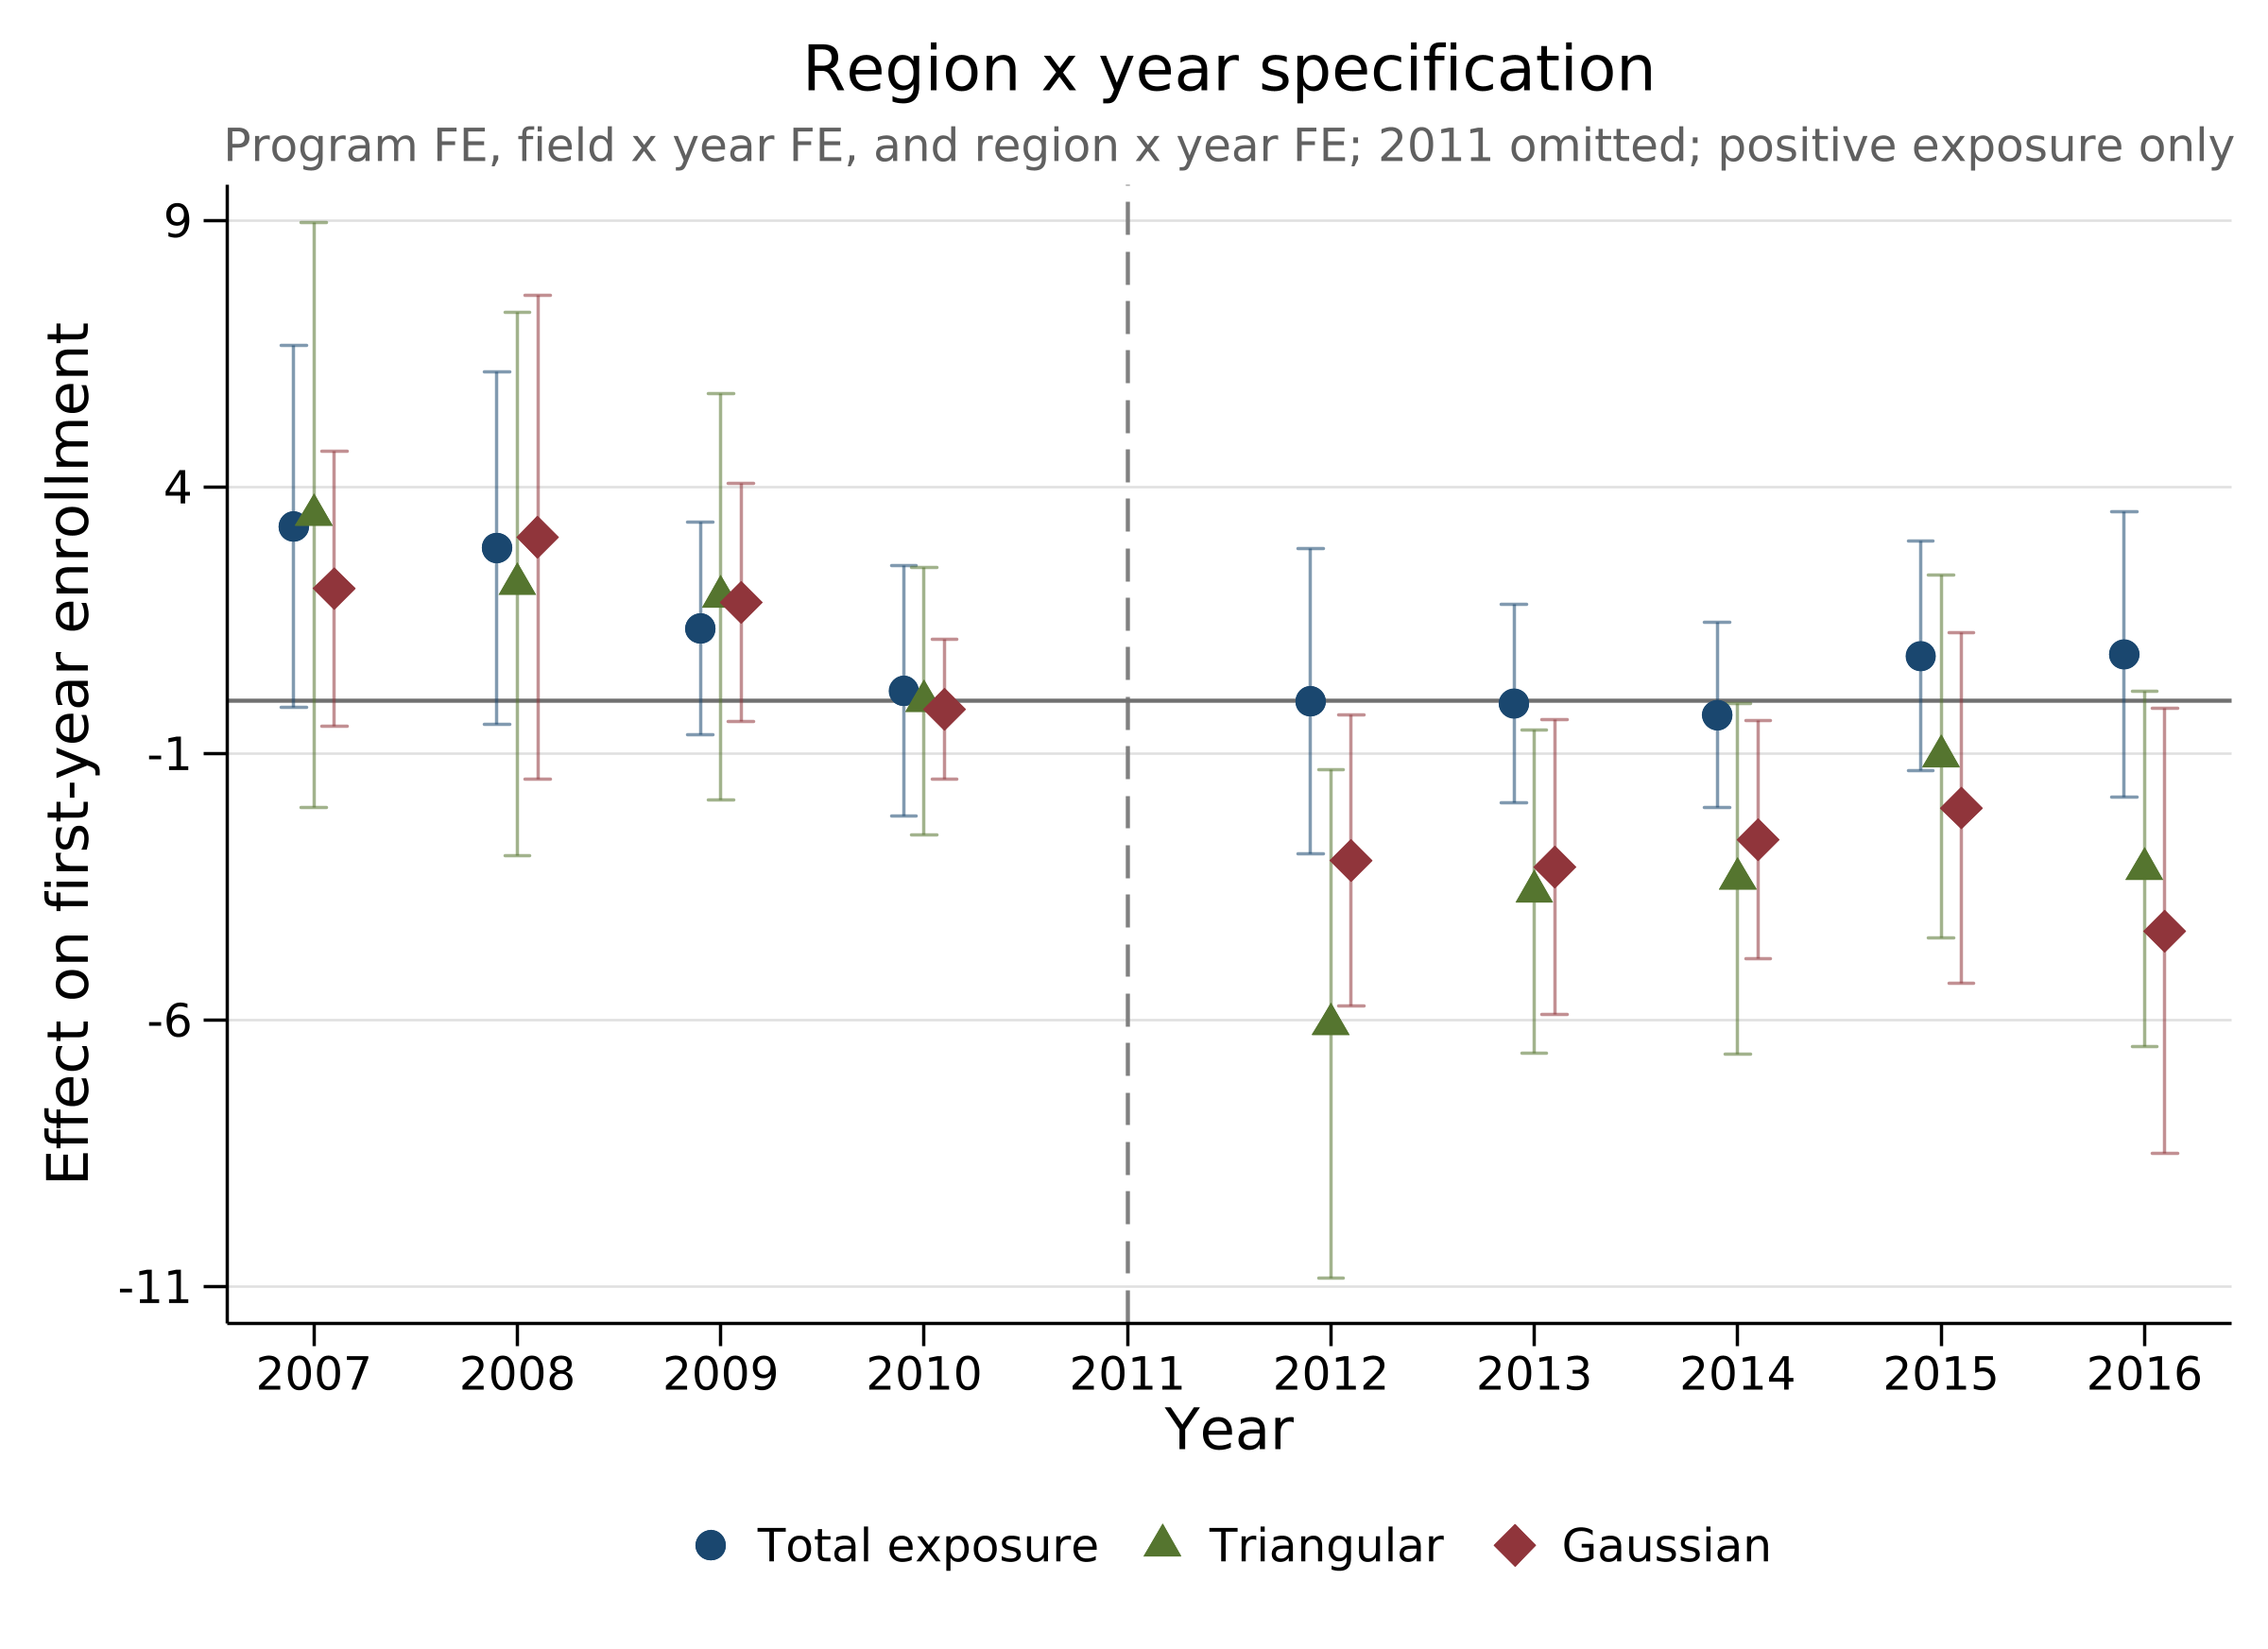
\includegraphics[width=\linewidth, height=0.66\textheight, keepaspectratio]{../../output/sua_event_study_exposure_comparison_regionyear_positive.png}
    \end{column}
\end{columns}

\vspace{0.04cm}

\begin{center}
\begin{minipage}{0.96\textwidth}
\tiny
\textit{Notes:}
Sample restricted to programs with positive exposure, defined separately for each measure (Triangular exposure can be zero where Total and Gaussian are positive). All such programs lie in the four regions with entrant programs, so the only difference with the entrant-region sample is that zero-exposure programs within those regions are dropped.
Broad-field markets; separate event studies for Total, Triangular and Gaussian
exposure. Coefficients measure the enrollment difference associated with a 10 percentage-point increase in exposure in each year relative to 2011. 95\% confidence intervals; SE clustered by pre-treatment market.
Joint pretrend $p$-values (2007--2010) for Total, Triangular and Gaussian are
0.072, 0.055 and 0.012 in the left panel, and 0.132, 0.348 and 0.207 in the right panel.
\end{minipage}
\end{center}

\end{frame}

%---------------------------------------------------------
\begin{frame}[label=sua-fs-log-entrant]

\frametitle{
    Log first stage: regions with entrant universities only
    \hfill
    \hyperlink{sua-log-first-stage}{\scriptsize\color{blue}$\leftarrow$ Main}
    \hyperlink{sua-es-log-entrant}{\scriptsize\color{blue}ES $\rightarrow$}
}

\centering

\vspace{-0.2cm}

{\small
\begin{equation*}
\log N^{\mathrm{first}}_{pt}
=
\beta_k\left[\widetilde{\log E_p^k}\times Post_t\right]
+\theta_k\left[D_p^k\times Post_t\right]
+\mu_p+\alpha_{f(p),t}+\gamma_{r(p),t}+\varepsilon_{pt}.
\end{equation*}
}

\vspace{-0.3cm}

\resizebox{0.62\textwidth}{!}{\begin{tabular}{lcccccc}
\toprule
 & \multicolumn{3}{c}{Field \(\times\) year FE} & \multicolumn{3}{c}{\(+\) Region \(\times\) year FE} \\
\cmidrule(lr){2-4}\cmidrule(lr){5-7}
Exposure measure & Broad & ISCED-97 & Generic & Broad & ISCED-97 & Generic \\
\midrule
\textit{Total} &  0.133\sym{***} &  0.109\sym{***} &  0.059\sym{*} &  0.025 &  0.012 &  0.006 \\
 & (0.039) & (0.035) & (0.031) & (0.086) & (0.041) & (0.031) \\
\quad Wald \(F\) & 11.66 &  9.63 &  3.51 &  0.09 &  0.09 &  0.04 \\
\quad Programs with zero exposure &        10 &        60 &       256 &        10 &        60 &       256 \\
\addlinespace
\textit{Triangular} & -0.015 &  0.006 &  0.029 & -0.052\sym{***} & -0.023 &  0.005 \\
 & (0.017) & (0.018) & (0.022) & (0.018) & (0.017) & (0.018) \\
\quad Wald \(F\) &  0.77 &  0.10 &  1.70 &  8.22 &  1.84 &  0.09 \\
\quad Programs with zero exposure &        96 &       192 &       416 &        96 &       192 &       416 \\
\addlinespace
\textit{Gaussian} & -0.024 & -0.009 &  0.019 & -0.117\sym{***} & -0.075\sym{**} & -0.021 \\
 & (0.036) & (0.034) & (0.019) & (0.034) & (0.031) & (0.017) \\
\quad Wald \(F\) &  0.44 &  0.06 &  0.96 & 11.57 &  5.83 &  1.46 \\
\quad Programs with zero exposure &        10 &        60 &       267 &        10 &        60 &       267 \\
\midrule
Observations &     5,090 &     5,080 &     4,781 &     5,090 &     5,080 &     4,781 \\
Programs &       601 &       601 &       571 &       601 &       601 &       571 \\
Markets &        40 &        80 &       303 &        40 &        80 &       303 \\
Regions &         4 &         4 &         4 &         4 &         4 &         4 \\
Program FE & Yes & Yes & Yes & Yes & Yes & Yes \\
Field \(\times\) year FE & Yes & Yes & Yes & Yes & Yes & Yes \\
Region \(\times\) year FE & No & No & No & Yes & Yes & Yes \\
\bottomrule
\end{tabular}
}

\vspace{0.05cm}

\parbox{0.97\textwidth}{%
\tiny
\textit{Notes:}
Sample restricted to incumbent programs in the four pre-treatment regions with entrant programs in 2009--2011 (Valpara\'iso, Biob\'io, La Araucan\'ia, Metropolitana); outside them exposure is zero by construction.
Same specification as the main log first stage: $\widetilde{\log E_p^k}=\log E_p^k$ if $E_p^k>0$ and 0 otherwise, $D_p^k=\mathbf{1}\{E_p^k>0\}$. Observations with zero first-year enrollment are excluded. SE clustered by pre-treatment market.
$^{***}p<0.01$, $^{**}p<0.05$, $^{*}p<0.10$.
}

\end{frame}

%---------------------------------------------------------
\begin{frame}[label=sua-es-log-entrant]

\frametitle{
    Log event studies: regions with entrant universities only
    \hfill
    \hyperlink{sua-fs-log-entrant}{\scriptsize\color{blue}$\leftarrow$ First stage}
}

\vspace{-0.12cm}

\begin{columns}[T,onlytextwidth]
    \begin{column}{0.495\textwidth}
        \centering
        \textbf{\scriptsize Field $\times$ year FE}

        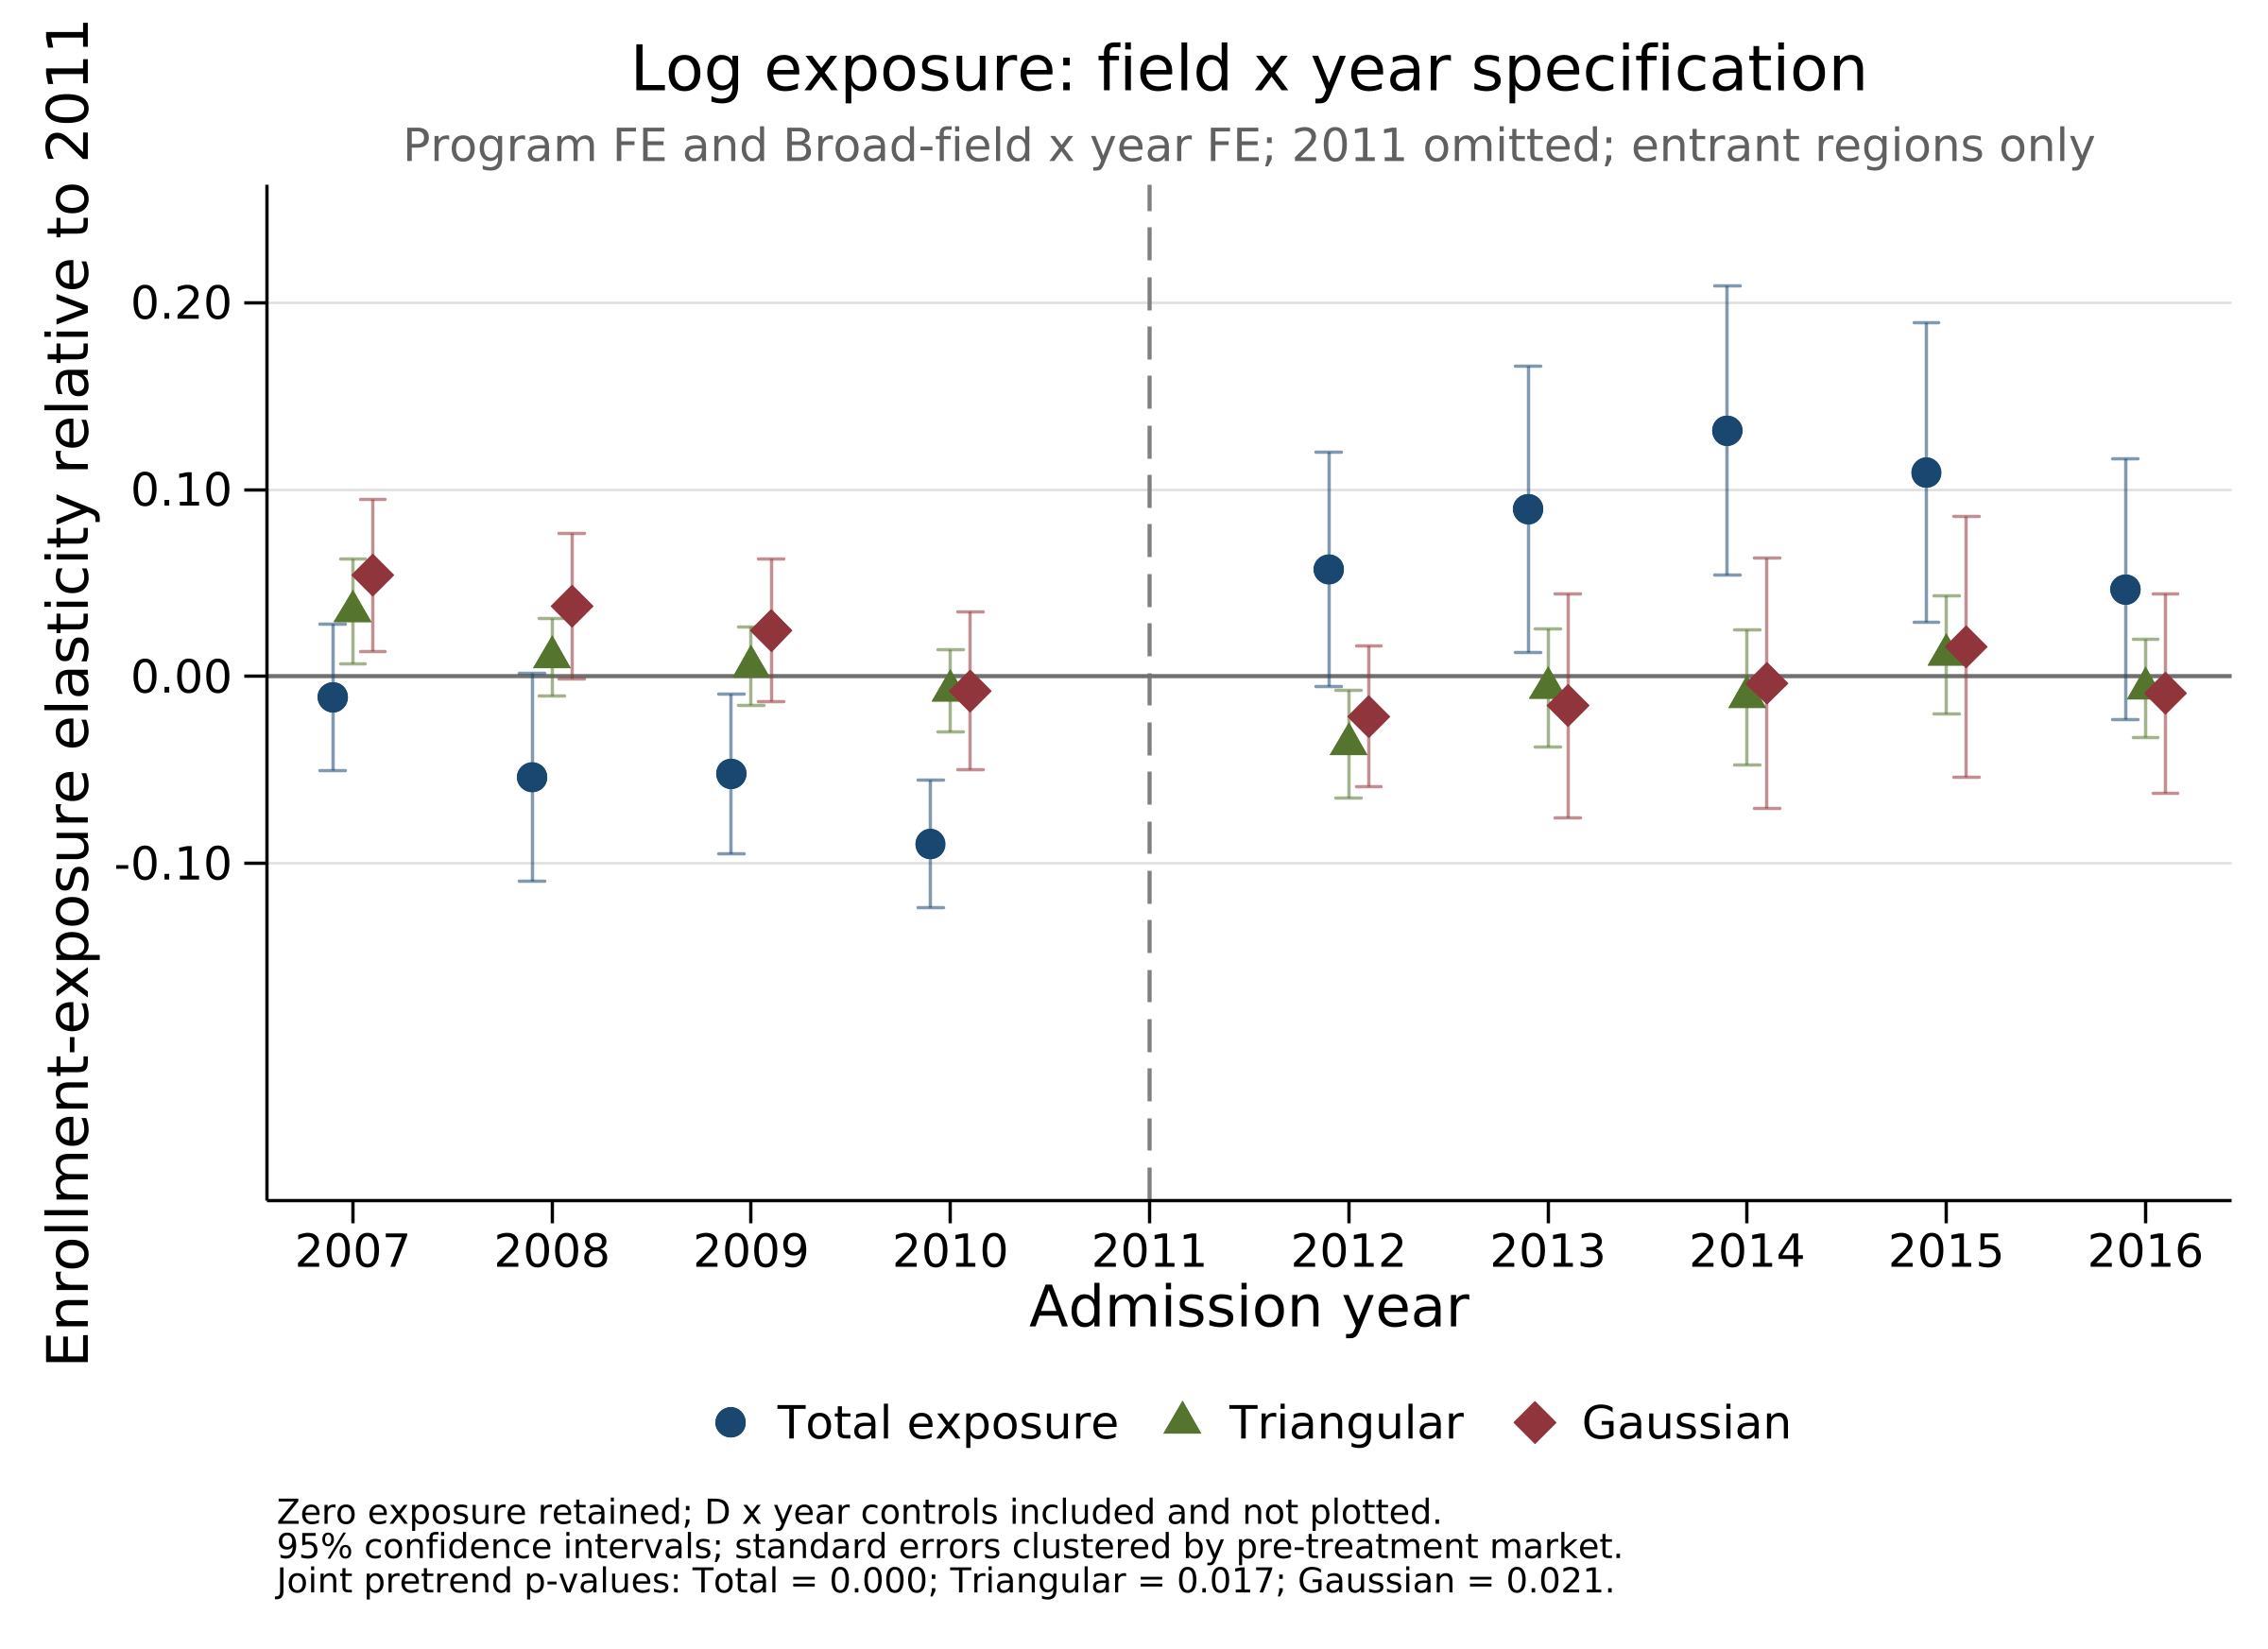
\includegraphics[width=\linewidth, height=0.66\textheight, keepaspectratio]{../../output/sua_log_event_study_baseline_entrant.png}
    \end{column}
    \begin{column}{0.495\textwidth}
        \centering
        \textbf{\scriptsize $+$ Region $\times$ year FE}

        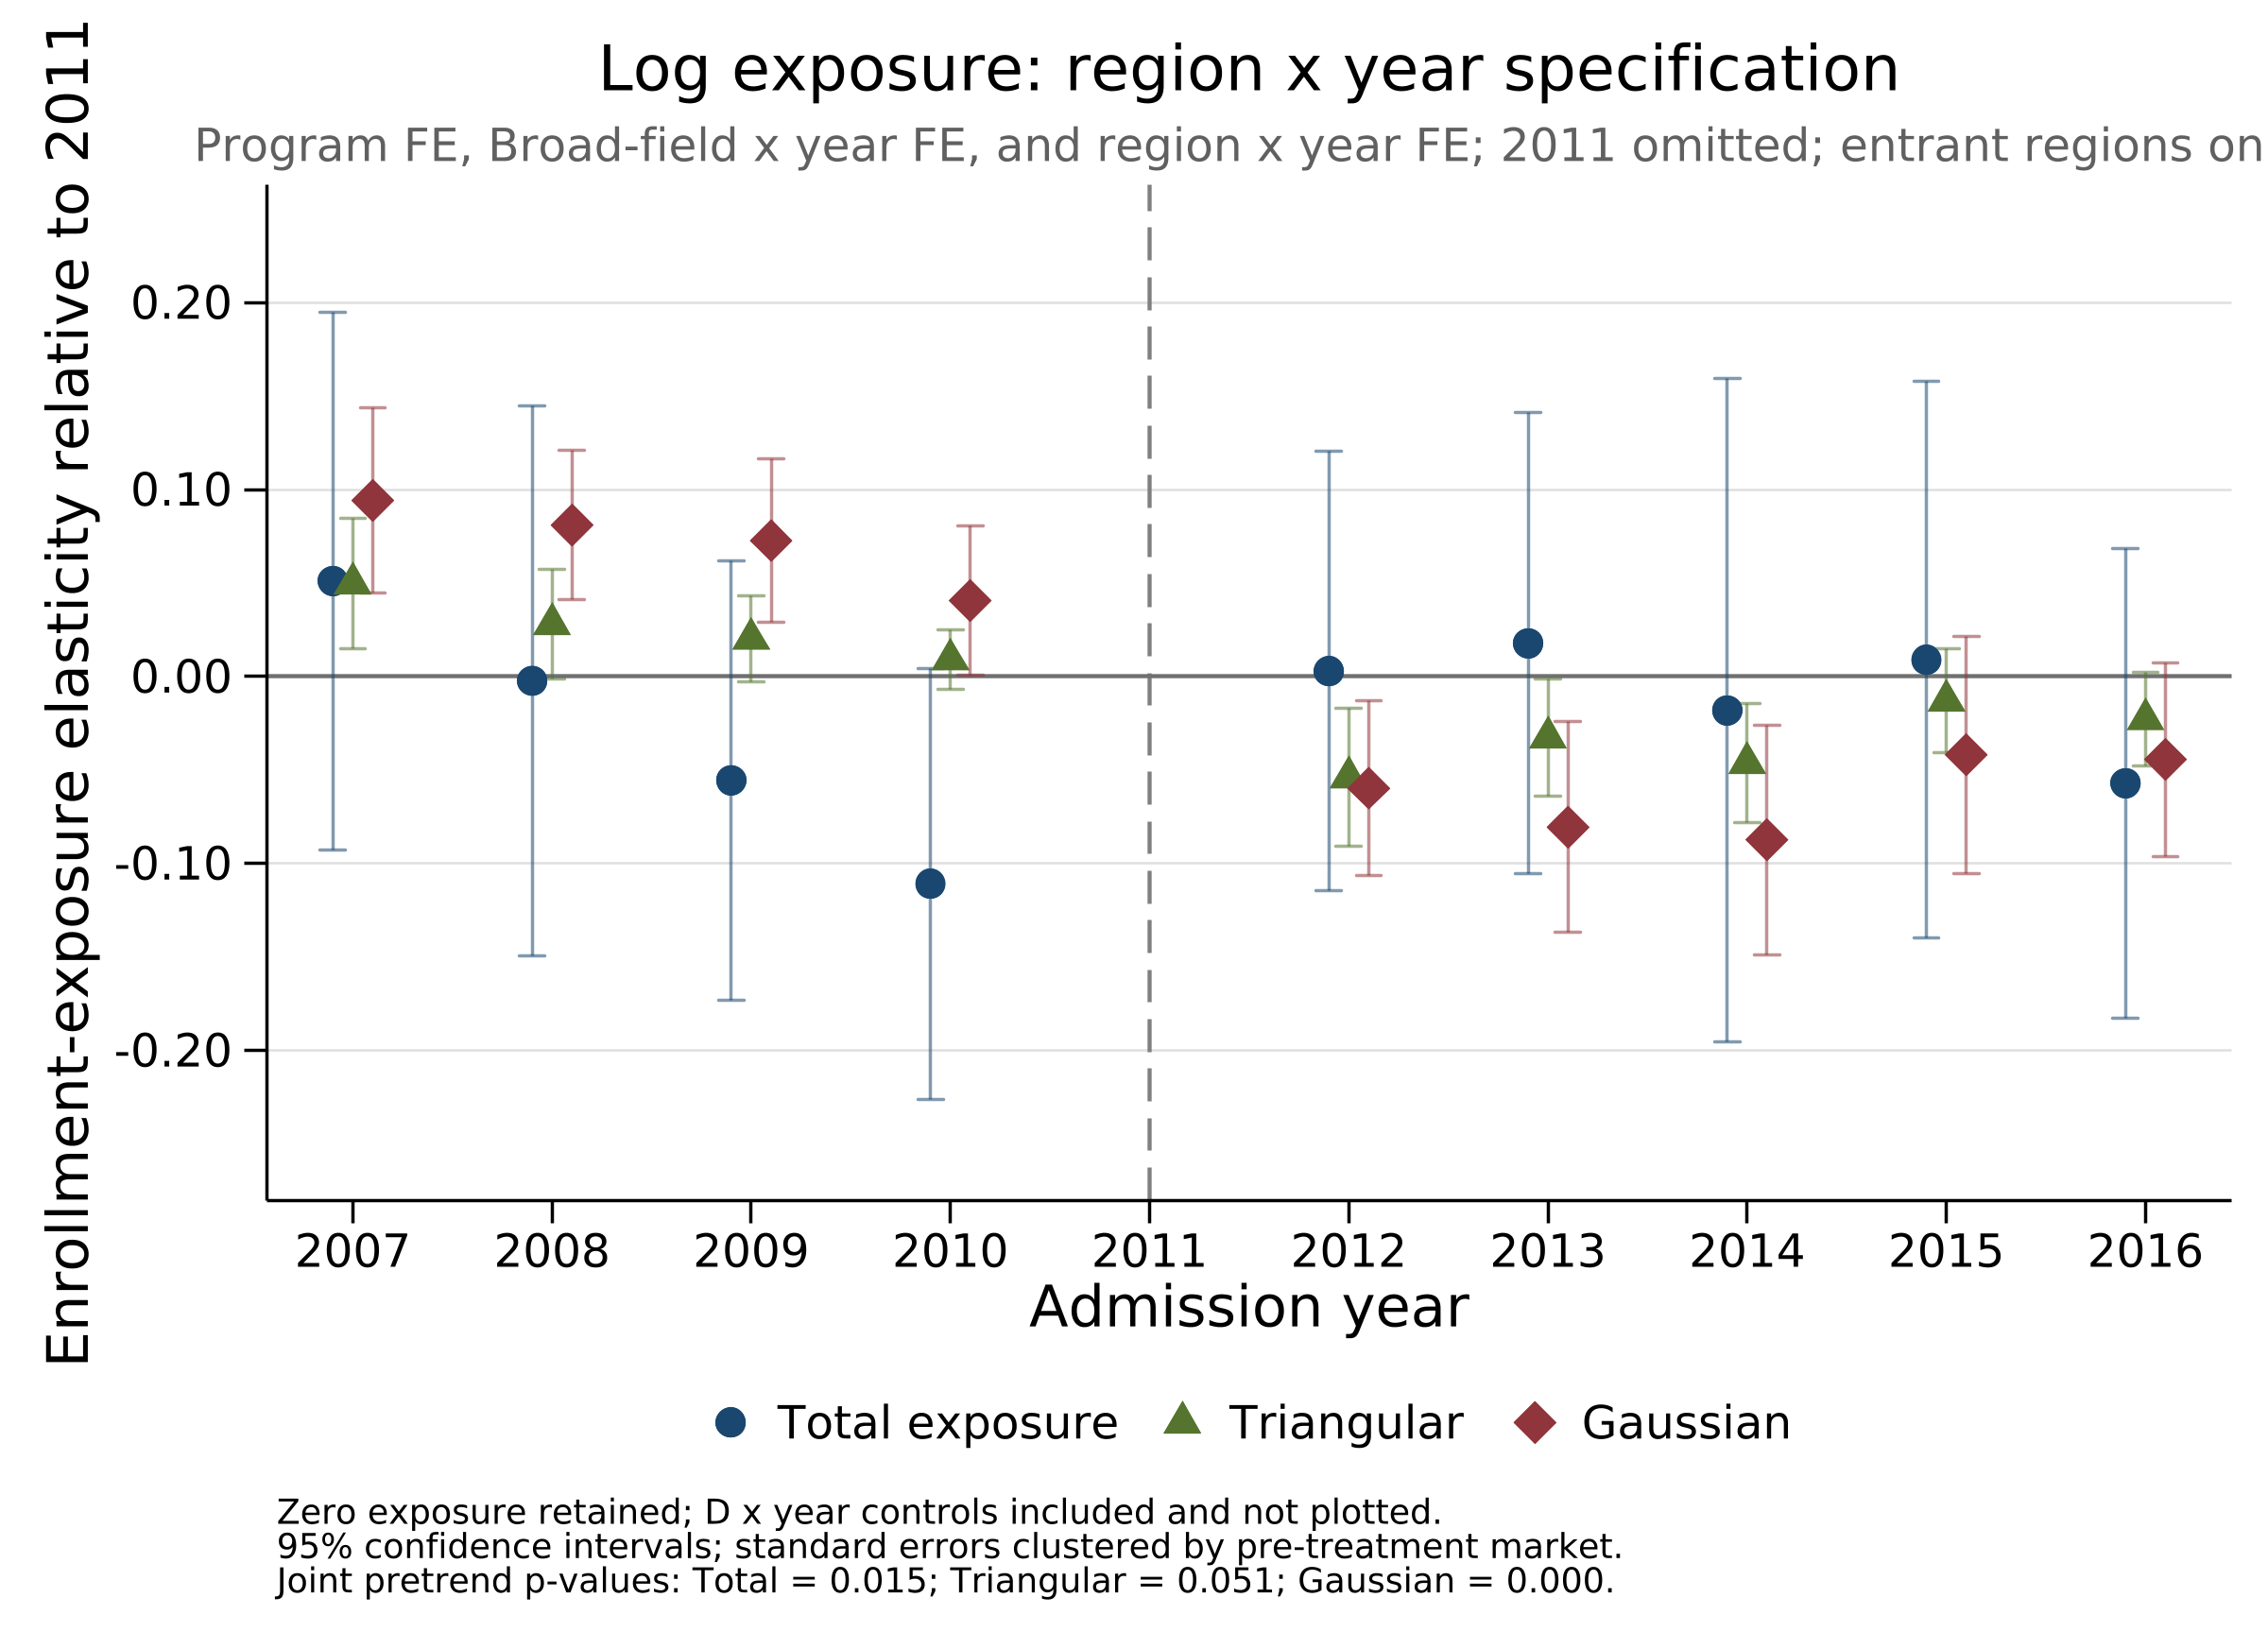
\includegraphics[width=\linewidth, height=0.66\textheight, keepaspectratio]{../../output/sua_log_event_study_regionyear_entrant.png}
    \end{column}
\end{columns}

\vspace{0.04cm}

\begin{center}
\begin{minipage}{0.96\textwidth}
\tiny
\textit{Notes:}
Sample restricted to incumbent programs in the four pre-treatment regions with entrant programs in 2009--2011 (Valpara\'iso, Biob\'io, La Araucan\'ia, Metropolitana); outside them exposure is zero by construction.
Broad-field markets; separate event studies for Total, Triangular and Gaussian
exposure. Plotted coefficients are those on the log-exposure $\times$ year terms, relative to 2011. 95\% confidence intervals; SE clustered by pre-treatment market.
Joint pretrend $p$-values (2007--2010) for Total, Triangular and Gaussian are
0.000, 0.018 and 0.021 in the left panel, and 0.015, 0.051 and 0.000 in the right panel.
\end{minipage}
\end{center}

\end{frame}

%---------------------------------------------------------
\begin{frame}[label=sua-fs-log-positive]

\frametitle{
    Log first stage: positive exposure only
    \hfill
    \hyperlink{sua-log-first-stage}{\scriptsize\color{blue}$\leftarrow$ Main}
    \hyperlink{sua-es-log-positive}{\scriptsize\color{blue}ES $\rightarrow$}
}

\centering

\vspace{-0.2cm}

{\small
\begin{equation*}
\log N^{\mathrm{first}}_{pt}
=
\beta_k\left[\log E_p^k\times Post_t\right]
+\mu_p+\alpha_{f(p),t}+\gamma_{r(p),t}+\varepsilon_{pt},
\qquad E_p^k>0.
\end{equation*}
}

\vspace{-0.3cm}

\resizebox{0.62\textwidth}{!}{\begin{tabular}{lcccccc}
\toprule
 & \multicolumn{3}{c}{Field \(\times\) year FE} & \multicolumn{3}{c}{\(+\) Region \(\times\) year FE} \\
\cmidrule(lr){2-4}\cmidrule(lr){5-7}
Exposure measure & Broad & ISCED-97 & Generic & Broad & ISCED-97 & Generic \\
\midrule
\textit{Total} &  0.132\sym{***} &  0.126\sym{***} &  0.134\sym{***} &  0.019 &  0.046 &  0.100\sym{***} \\
 & (0.039) & (0.036) & (0.021) & (0.086) & (0.061) & (0.024) \\
\quad Wald \(F\) & 11.39 & 12.01 & 41.28 &  0.05 &  0.58 & 17.13 \\
\quad Programs &       591 &       540 &       304 &       591 &       540 &       304 \\
\addlinespace
\textit{Triangular} & -0.015 &  0.004 &  0.021 & -0.056\sym{***} & -0.028 &  0.004 \\
 & (0.019) & (0.022) & (0.027) & (0.020) & (0.021) & (0.023) \\
\quad Wald \(F\) &  0.61 &  0.03 &  0.56 &  8.06 &  1.84 &  0.03 \\
\quad Programs &       505 &       407 &       142 &       505 &       407 &       142 \\
\addlinespace
\textit{Gaussian} & -0.025 & -0.004 &  0.018 & -0.117\sym{***} & -0.078\sym{**} & -0.026 \\
 & (0.037) & (0.036) & (0.022) & (0.034) & (0.035) & (0.020) \\
\quad Wald \(F\) &  0.46 &  0.01 &  0.64 & 11.55 &  4.97 &  1.79 \\
\quad Programs &       591 &       540 &       292 &       591 &       540 &       292 \\
\midrule
Observations (Total) &     5,009 &     4,571 &     2,516 &     5,009 &     4,571 &     2,516 \\
Programs (Total) &       591 &       540 &       304 &       591 &       540 &       304 \\
Markets (Total) &        36 &        59 &       131 &        36 &        59 &       131 \\
Regions &         4 &         4 &         4 &         4 &         4 &         4 \\
Program FE & Yes & Yes & Yes & Yes & Yes & Yes \\
Field \(\times\) year FE & Yes & Yes & Yes & Yes & Yes & Yes \\
Region \(\times\) year FE & No & No & No & Yes & Yes & Yes \\
\bottomrule
\end{tabular}
}

\vspace{0.05cm}

\parbox{0.97\textwidth}{%
\tiny
\textit{Notes:}
Sample restricted to programs with positive exposure, defined separately for each measure (Triangular exposure can be zero where Total and Gaussian are positive). All such programs lie in the four regions with entrant programs, so the only difference with the entrant-region sample is that zero-exposure programs within those regions are dropped.
Log first stage without zero-exposure programs, so $D_p^k\times Post_t$ equals $Post_t$ and is absorbed by the fixed effects. Observations with zero first-year enrollment are excluded. SE clustered by pre-treatment market.
$^{***}p<0.01$, $^{**}p<0.05$, $^{*}p<0.10$.
}

\end{frame}

%---------------------------------------------------------
\begin{frame}[label=sua-es-log-positive]

\frametitle{
    Log event studies: positive exposure only
    \hfill
    \hyperlink{sua-fs-log-positive}{\scriptsize\color{blue}$\leftarrow$ First stage}
}

\vspace{-0.12cm}

\begin{columns}[T,onlytextwidth]
    \begin{column}{0.495\textwidth}
        \centering
        \textbf{\scriptsize Field $\times$ year FE}

        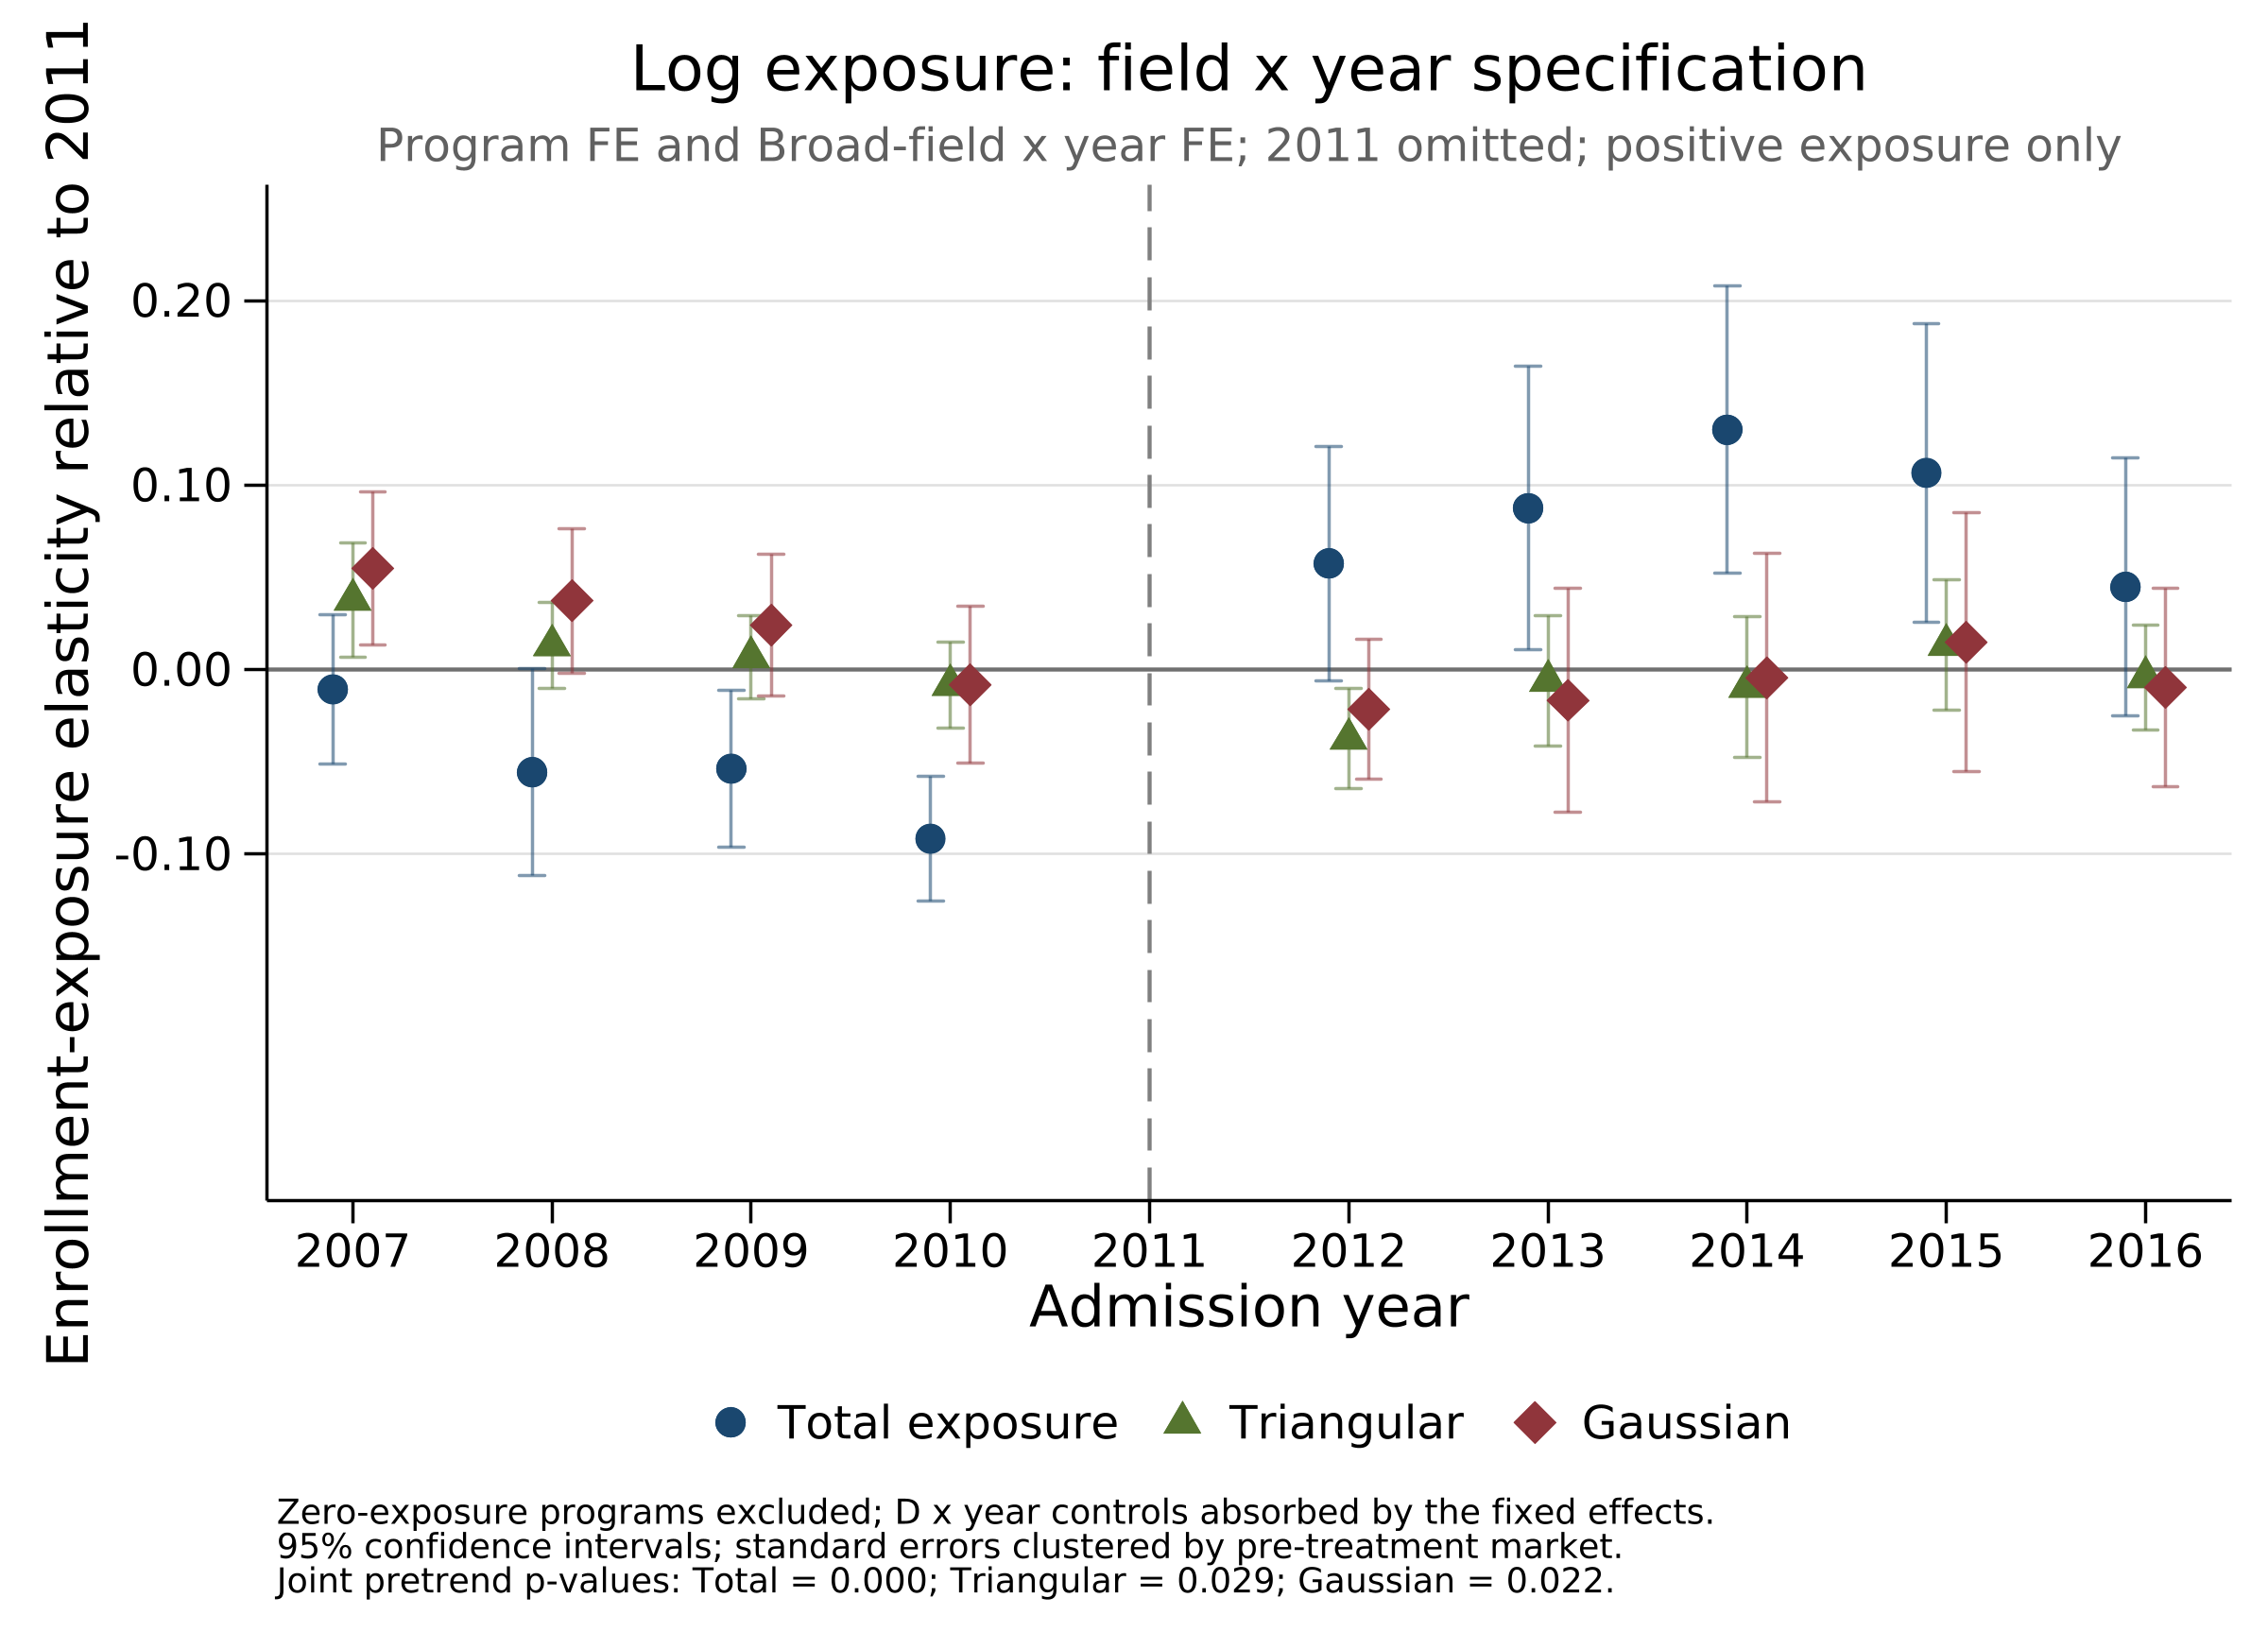
\includegraphics[width=\linewidth, height=0.66\textheight, keepaspectratio]{../../output/sua_log_event_study_baseline_positive.png}
    \end{column}
    \begin{column}{0.495\textwidth}
        \centering
        \textbf{\scriptsize $+$ Region $\times$ year FE}

        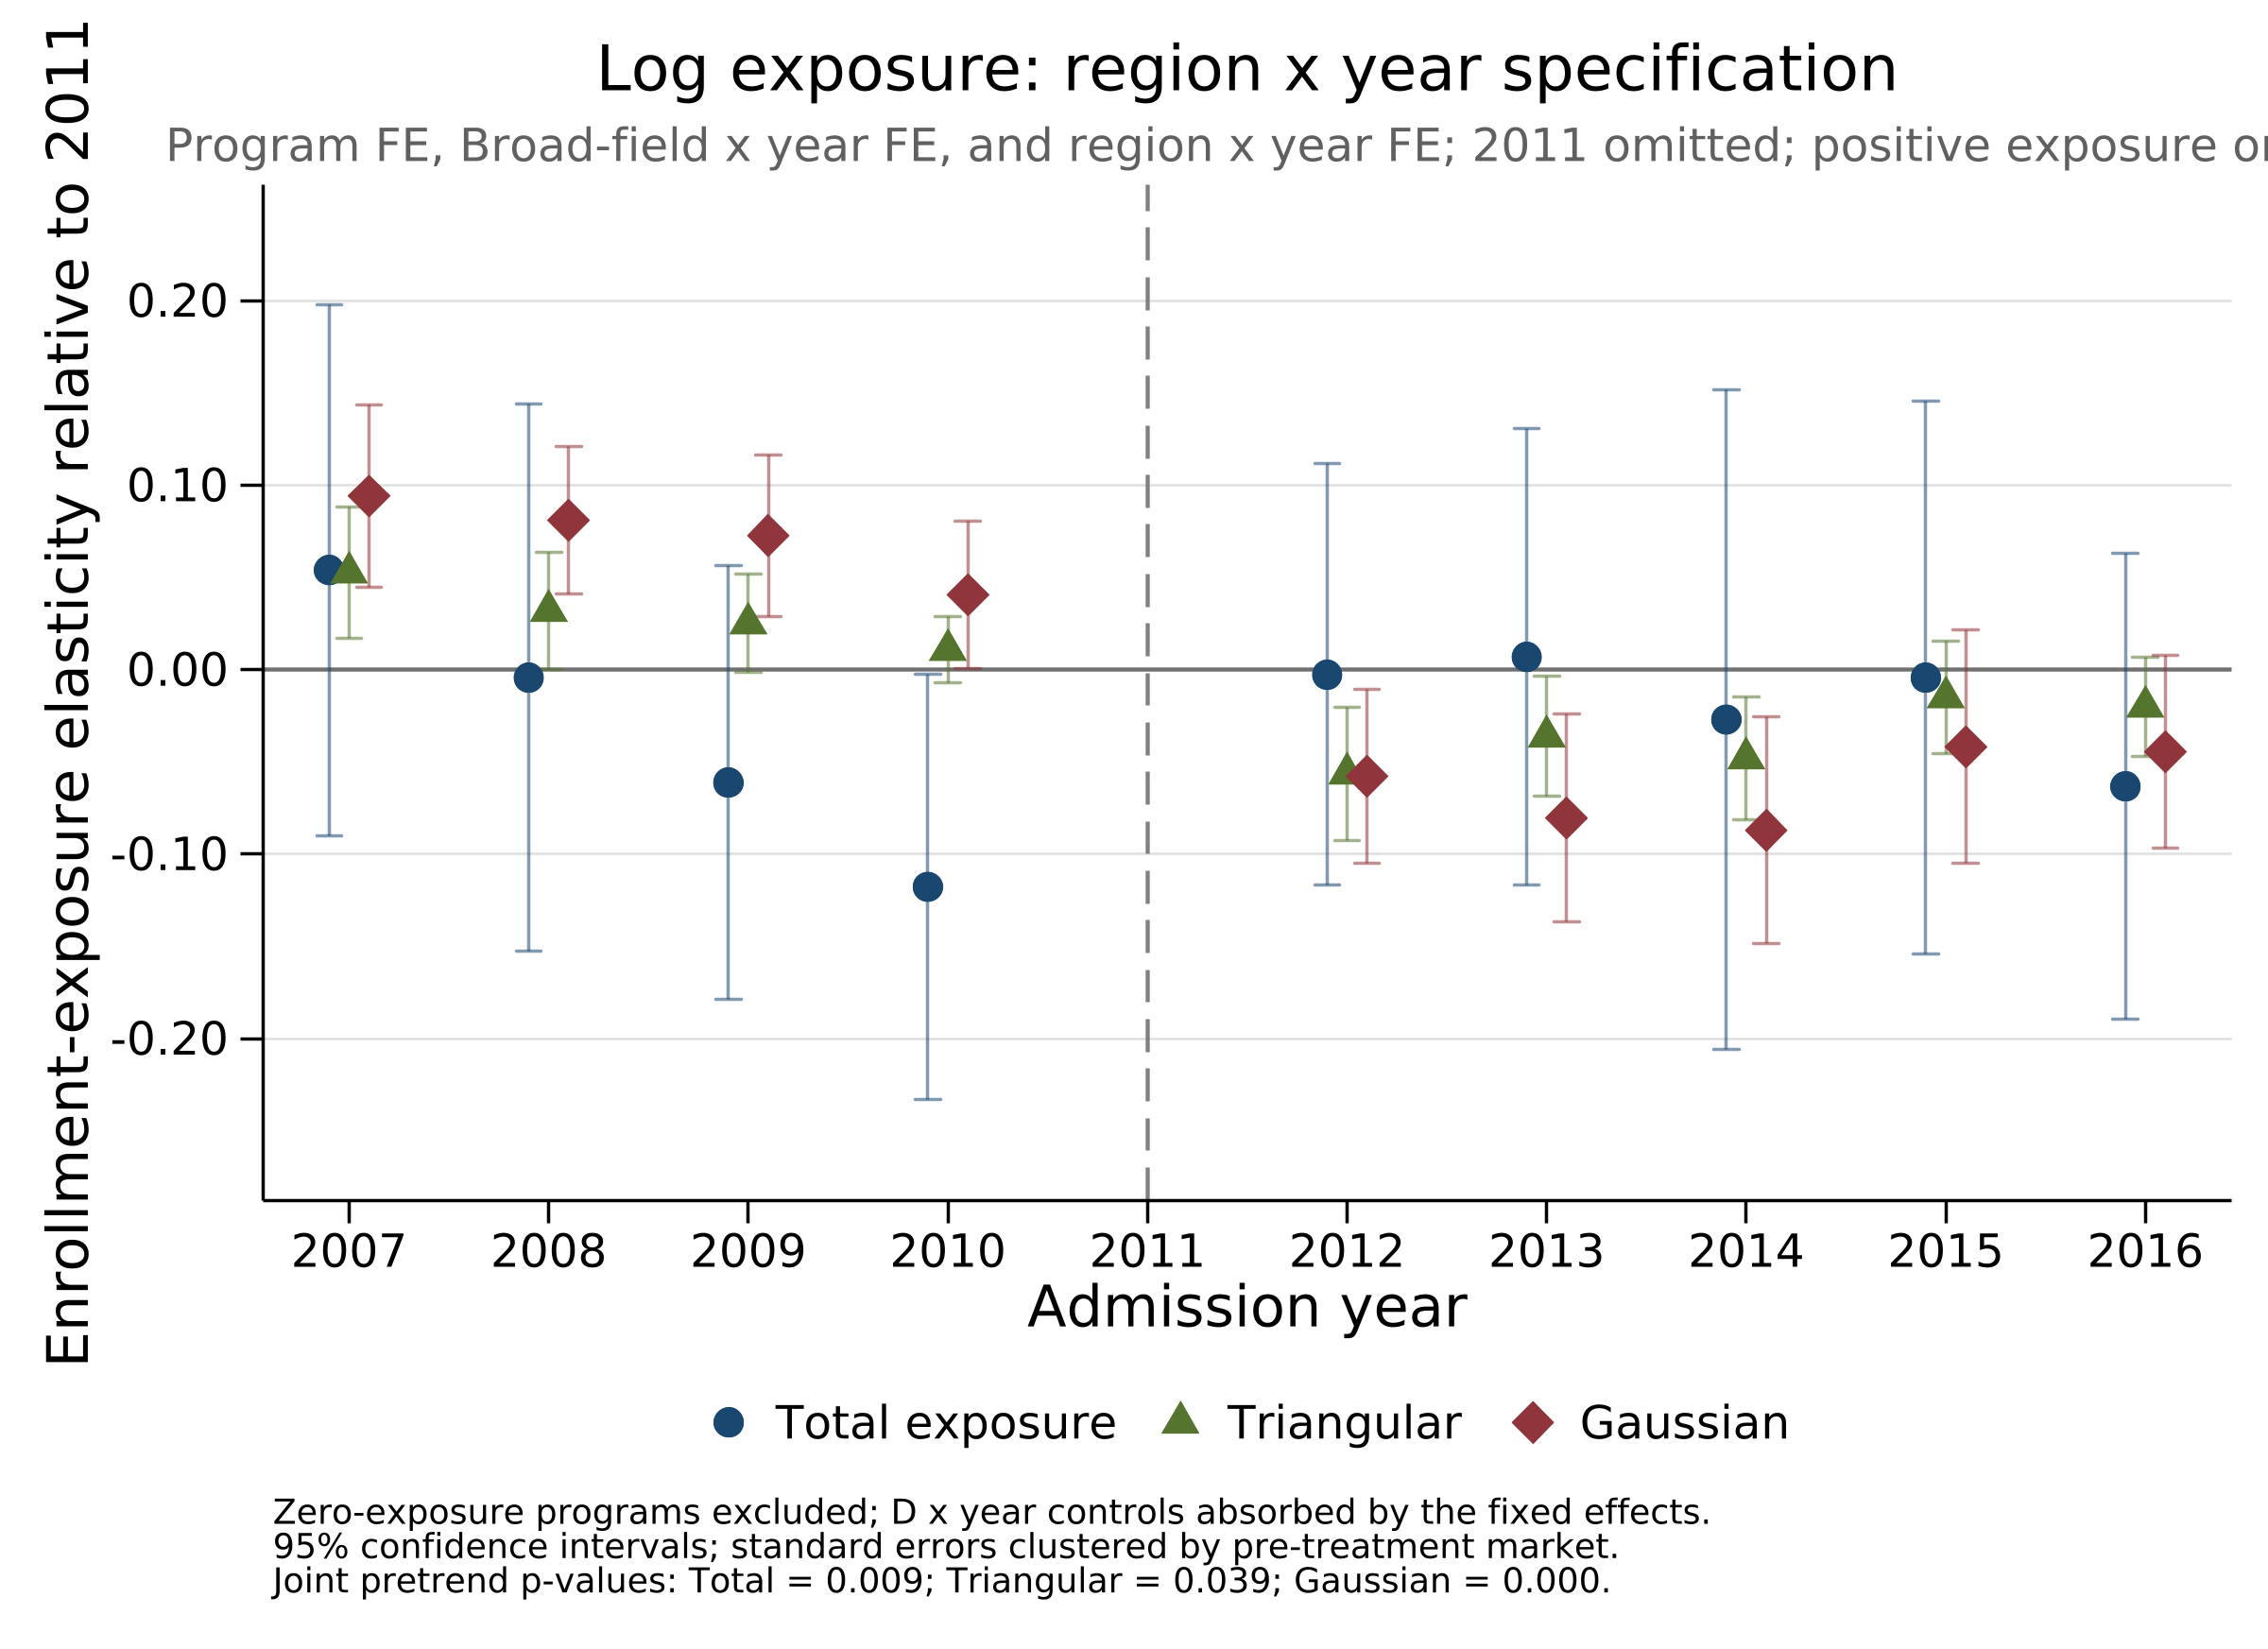
\includegraphics[width=\linewidth, height=0.66\textheight, keepaspectratio]{../../output/sua_log_event_study_regionyear_positive.png}
    \end{column}
\end{columns}

\vspace{0.04cm}

\begin{center}
\begin{minipage}{0.96\textwidth}
\tiny
\textit{Notes:}
Sample restricted to programs with positive exposure, defined separately for each measure (Triangular exposure can be zero where Total and Gaussian are positive). All such programs lie in the four regions with entrant programs, so the only difference with the entrant-region sample is that zero-exposure programs within those regions are dropped.
Broad-field markets; separate event studies for Total, Triangular and Gaussian
exposure. Plotted coefficients are those on the log-exposure $\times$ year terms, relative to 2011. 95\% confidence intervals; SE clustered by pre-treatment market.
Joint pretrend $p$-values (2007--2010) for Total, Triangular and Gaussian are
0.000, 0.029 and 0.022 in the left panel, and 0.009, 0.039 and 0.000 in the right panel.
\end{minipage}
\end{center}

\end{frame}

%---------------------------------------------------------
\begin{frame}[label=sua-event-studies]

\frametitle{
    SUA exposure: event-study estimates
    \hfill
    \hyperlink{sua-first-stage}{
        \scriptsize\color{blue}
        $\leftarrow$ First stage
    }
}

\vspace{-0.12cm}

\begin{columns}[T,onlytextwidth]

    \begin{column}{0.495\textwidth}
        \centering

                \textbf{\scriptsize Field $\times$ year FE}

        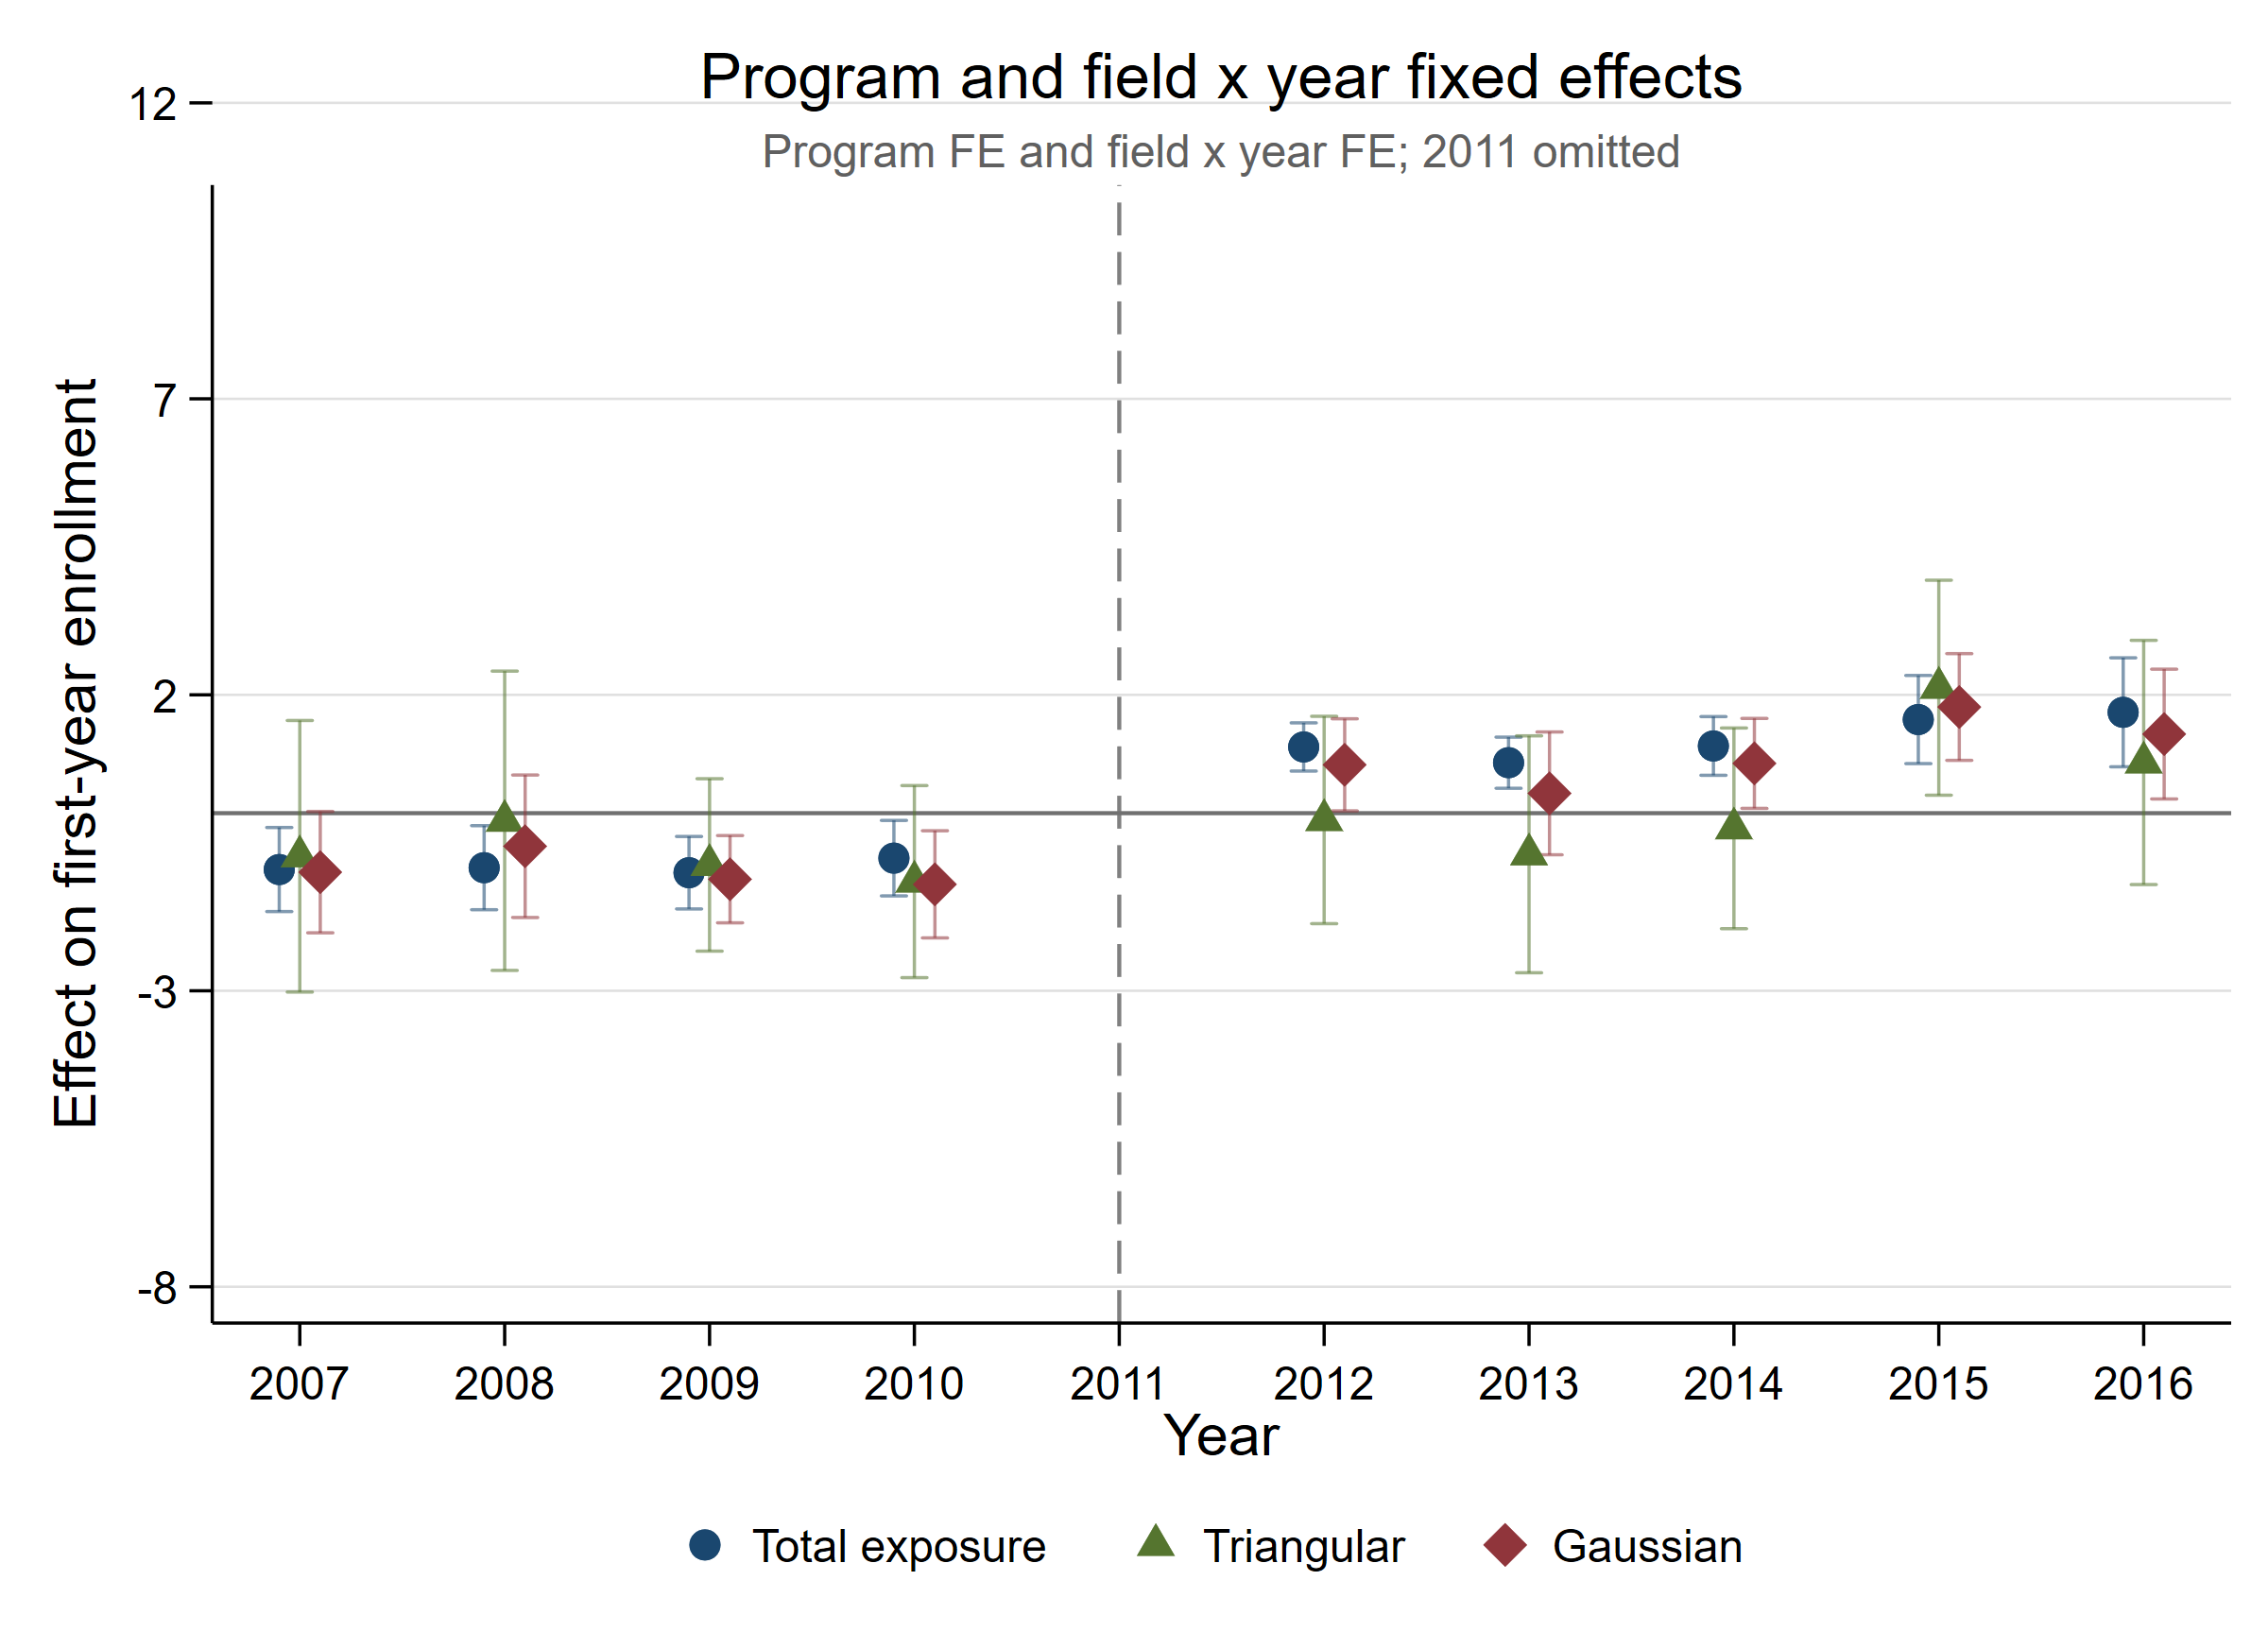
\includegraphics[ width=\linewidth, height=0.68\textheight, keepaspectratio ]{../../output/sua_event_study_exposure_comparison_baseline.png}

        \vspace{-0.08cm}

    \end{column}

    \begin{column}{0.495\textwidth}
        \centering
                \textbf{\scriptsize $+$ Region $\times$ year FE}


        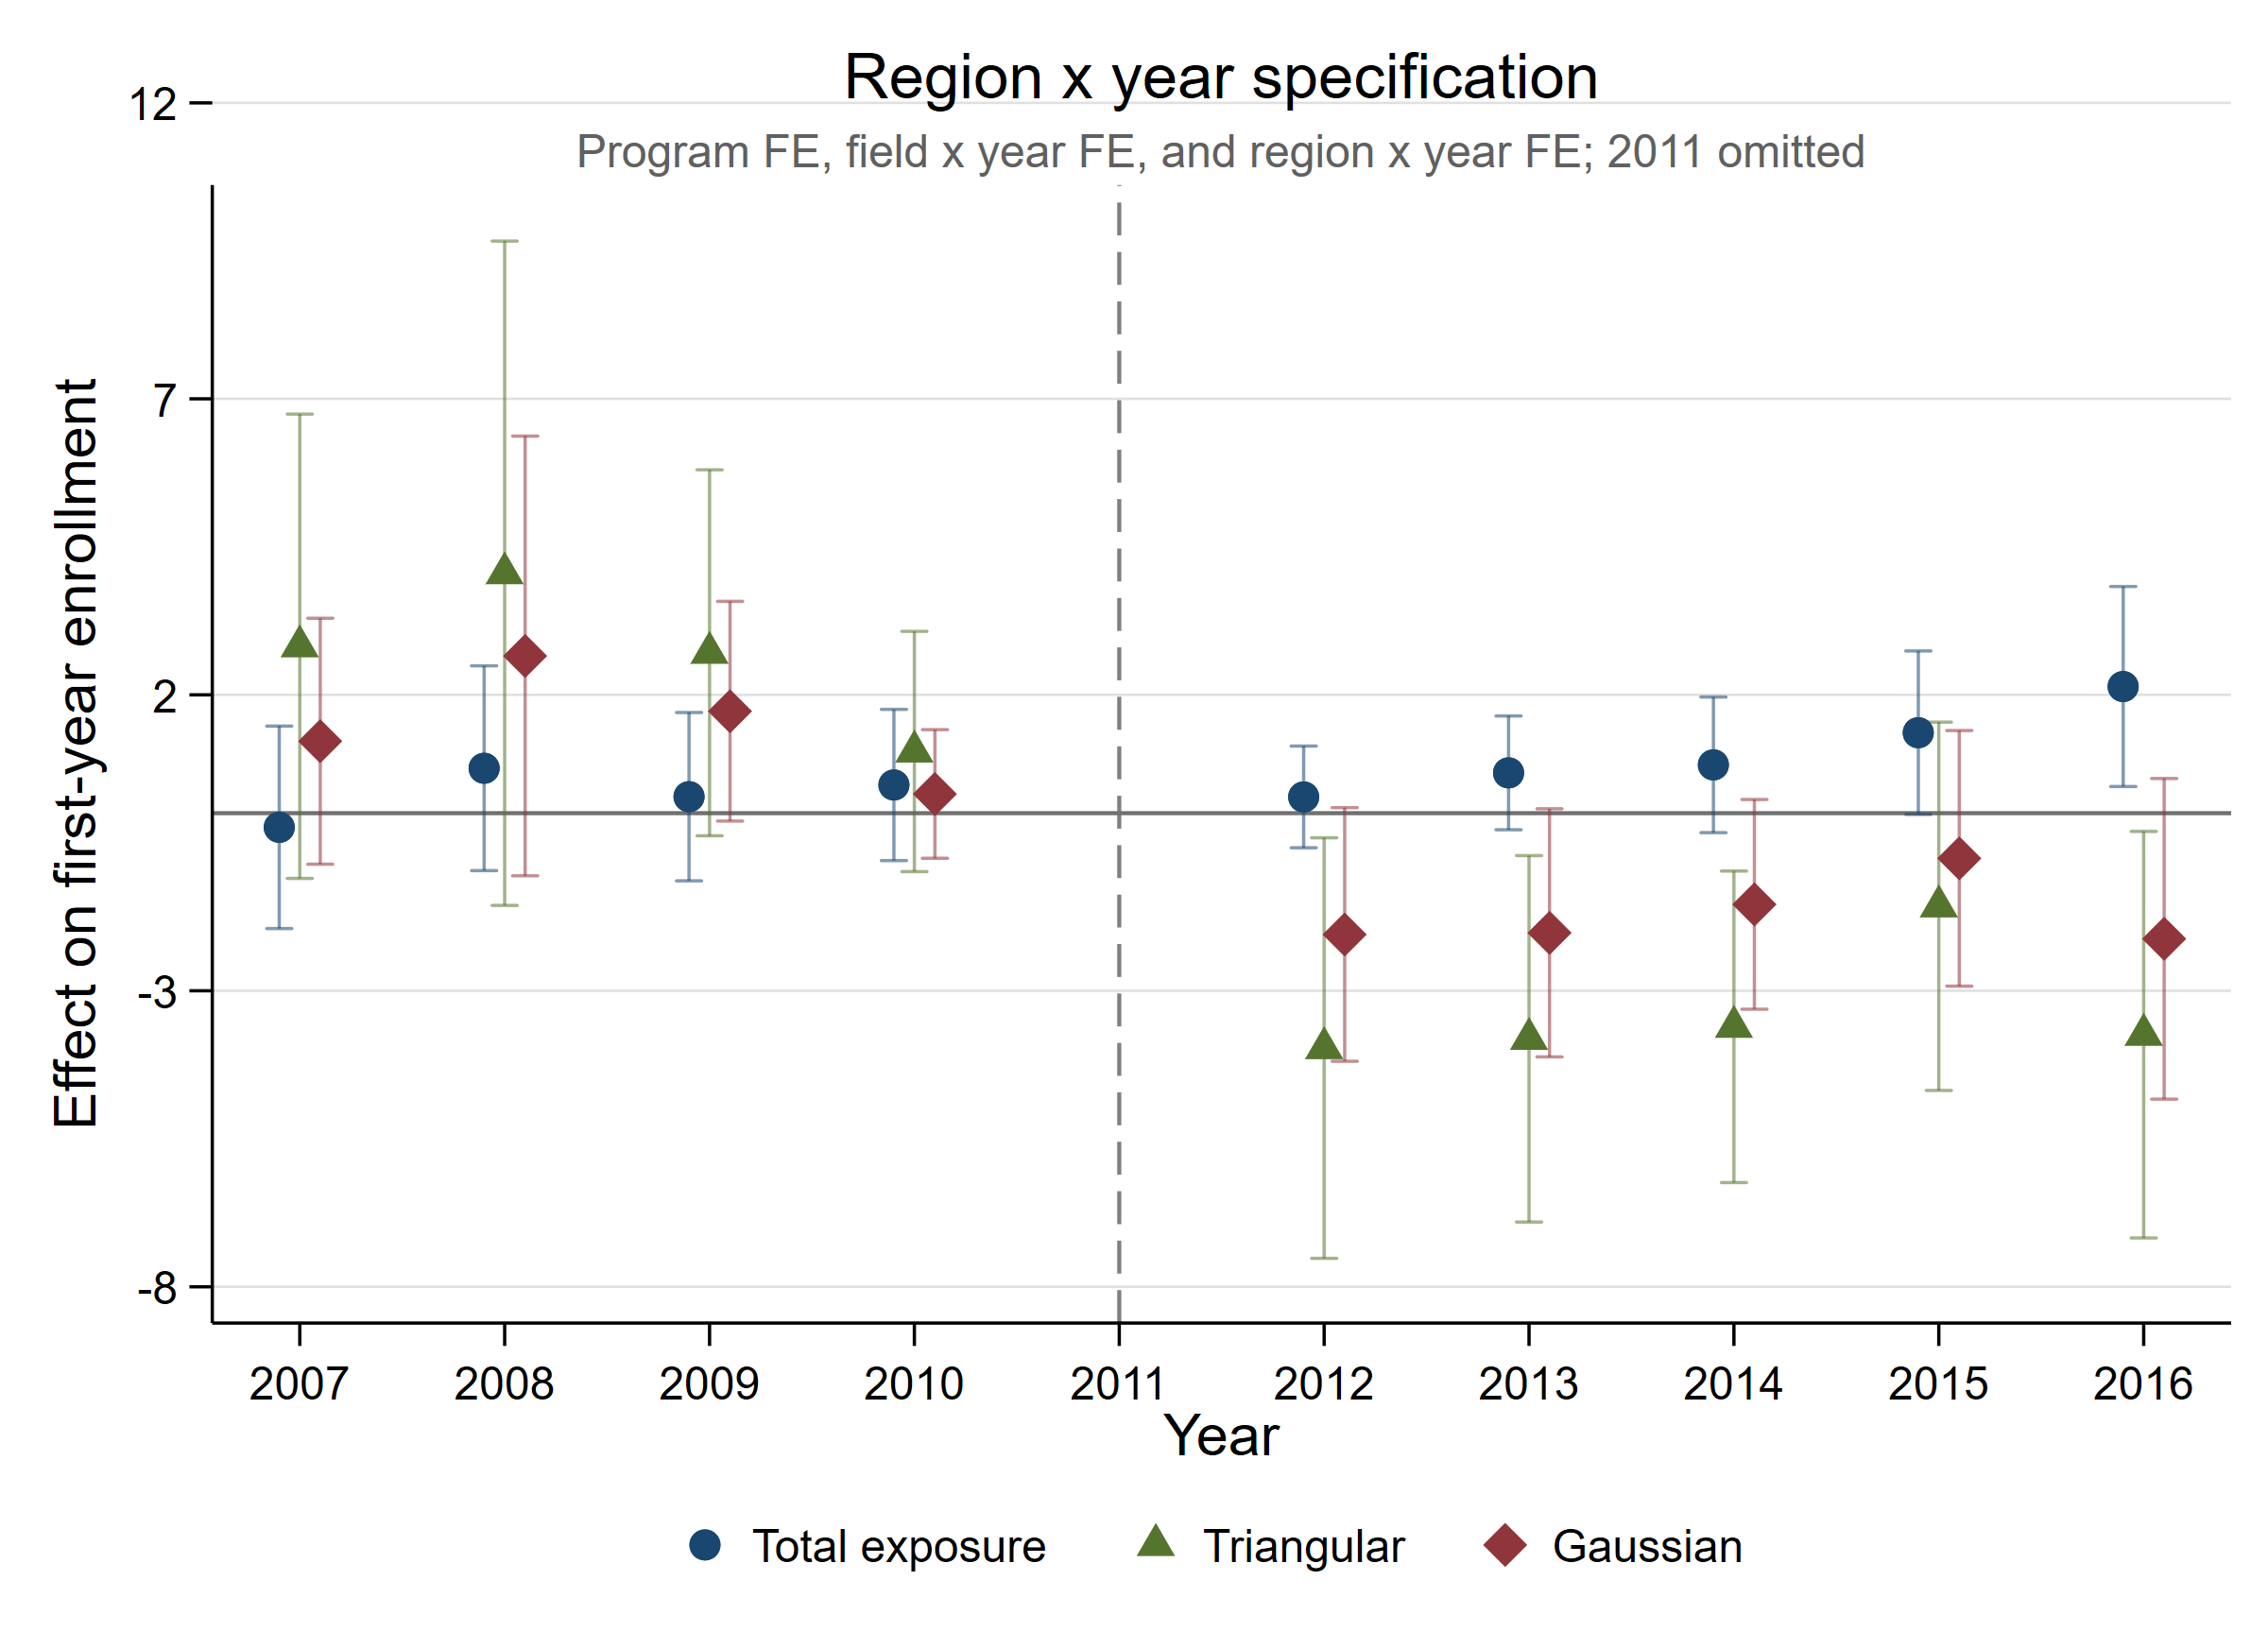
\includegraphics[ width=\linewidth, height=0.68\textheight, keepaspectratio ]{../../output/sua_event_study_exposure_comparison_regionyear.png}

        \vspace{-0.08cm}

    \end{column}

\end{columns}

\vspace{0.04cm}

\begin{center}
\begin{minipage}{0.96\textwidth}
\tiny
\textit{Notes:}
The figures use the Broad-field market definition and report separate event
studies for Total, Triangular and Gaussian exposure. The left panel absorbs
program and Broad-field $\times$ year fixed effects. The right panel
additionally absorbs pre-treatment region $\times$ year fixed effects.
Coefficients measure the enrollment difference associated with a
10 percentage-point increase in exposure in each year relative to 2011,
the omitted year. Vertical bars report 95\% confidence intervals and
standard errors are clustered by the pre-treatment market. Joint pretrend
$p$-values for Total, Triangular and Gaussian exposure are 0.024, 0.568 and
0.020 in the left panel, and 0.285, 0.385 and 0.368 in the right panel.
\end{minipage}
\end{center}

\end{frame}
%---------------------------------------------------------
\begin{frame}[label=sua-log-event-studies]

\frametitle{
SUA exposure: log event-study estimates
\hfill
\hyperlink{sua-log-first-stage}{
\scriptsize\color{blue}
$\leftarrow$ Log first stage
}
}

\vspace{-0.10cm}

\begin{columns}[T,onlytextwidth]

\begin{column}{0.495\textwidth}
    \centering

    \textbf{\scriptsize Field $\times$ year FE}

    \vspace{0.03cm}

    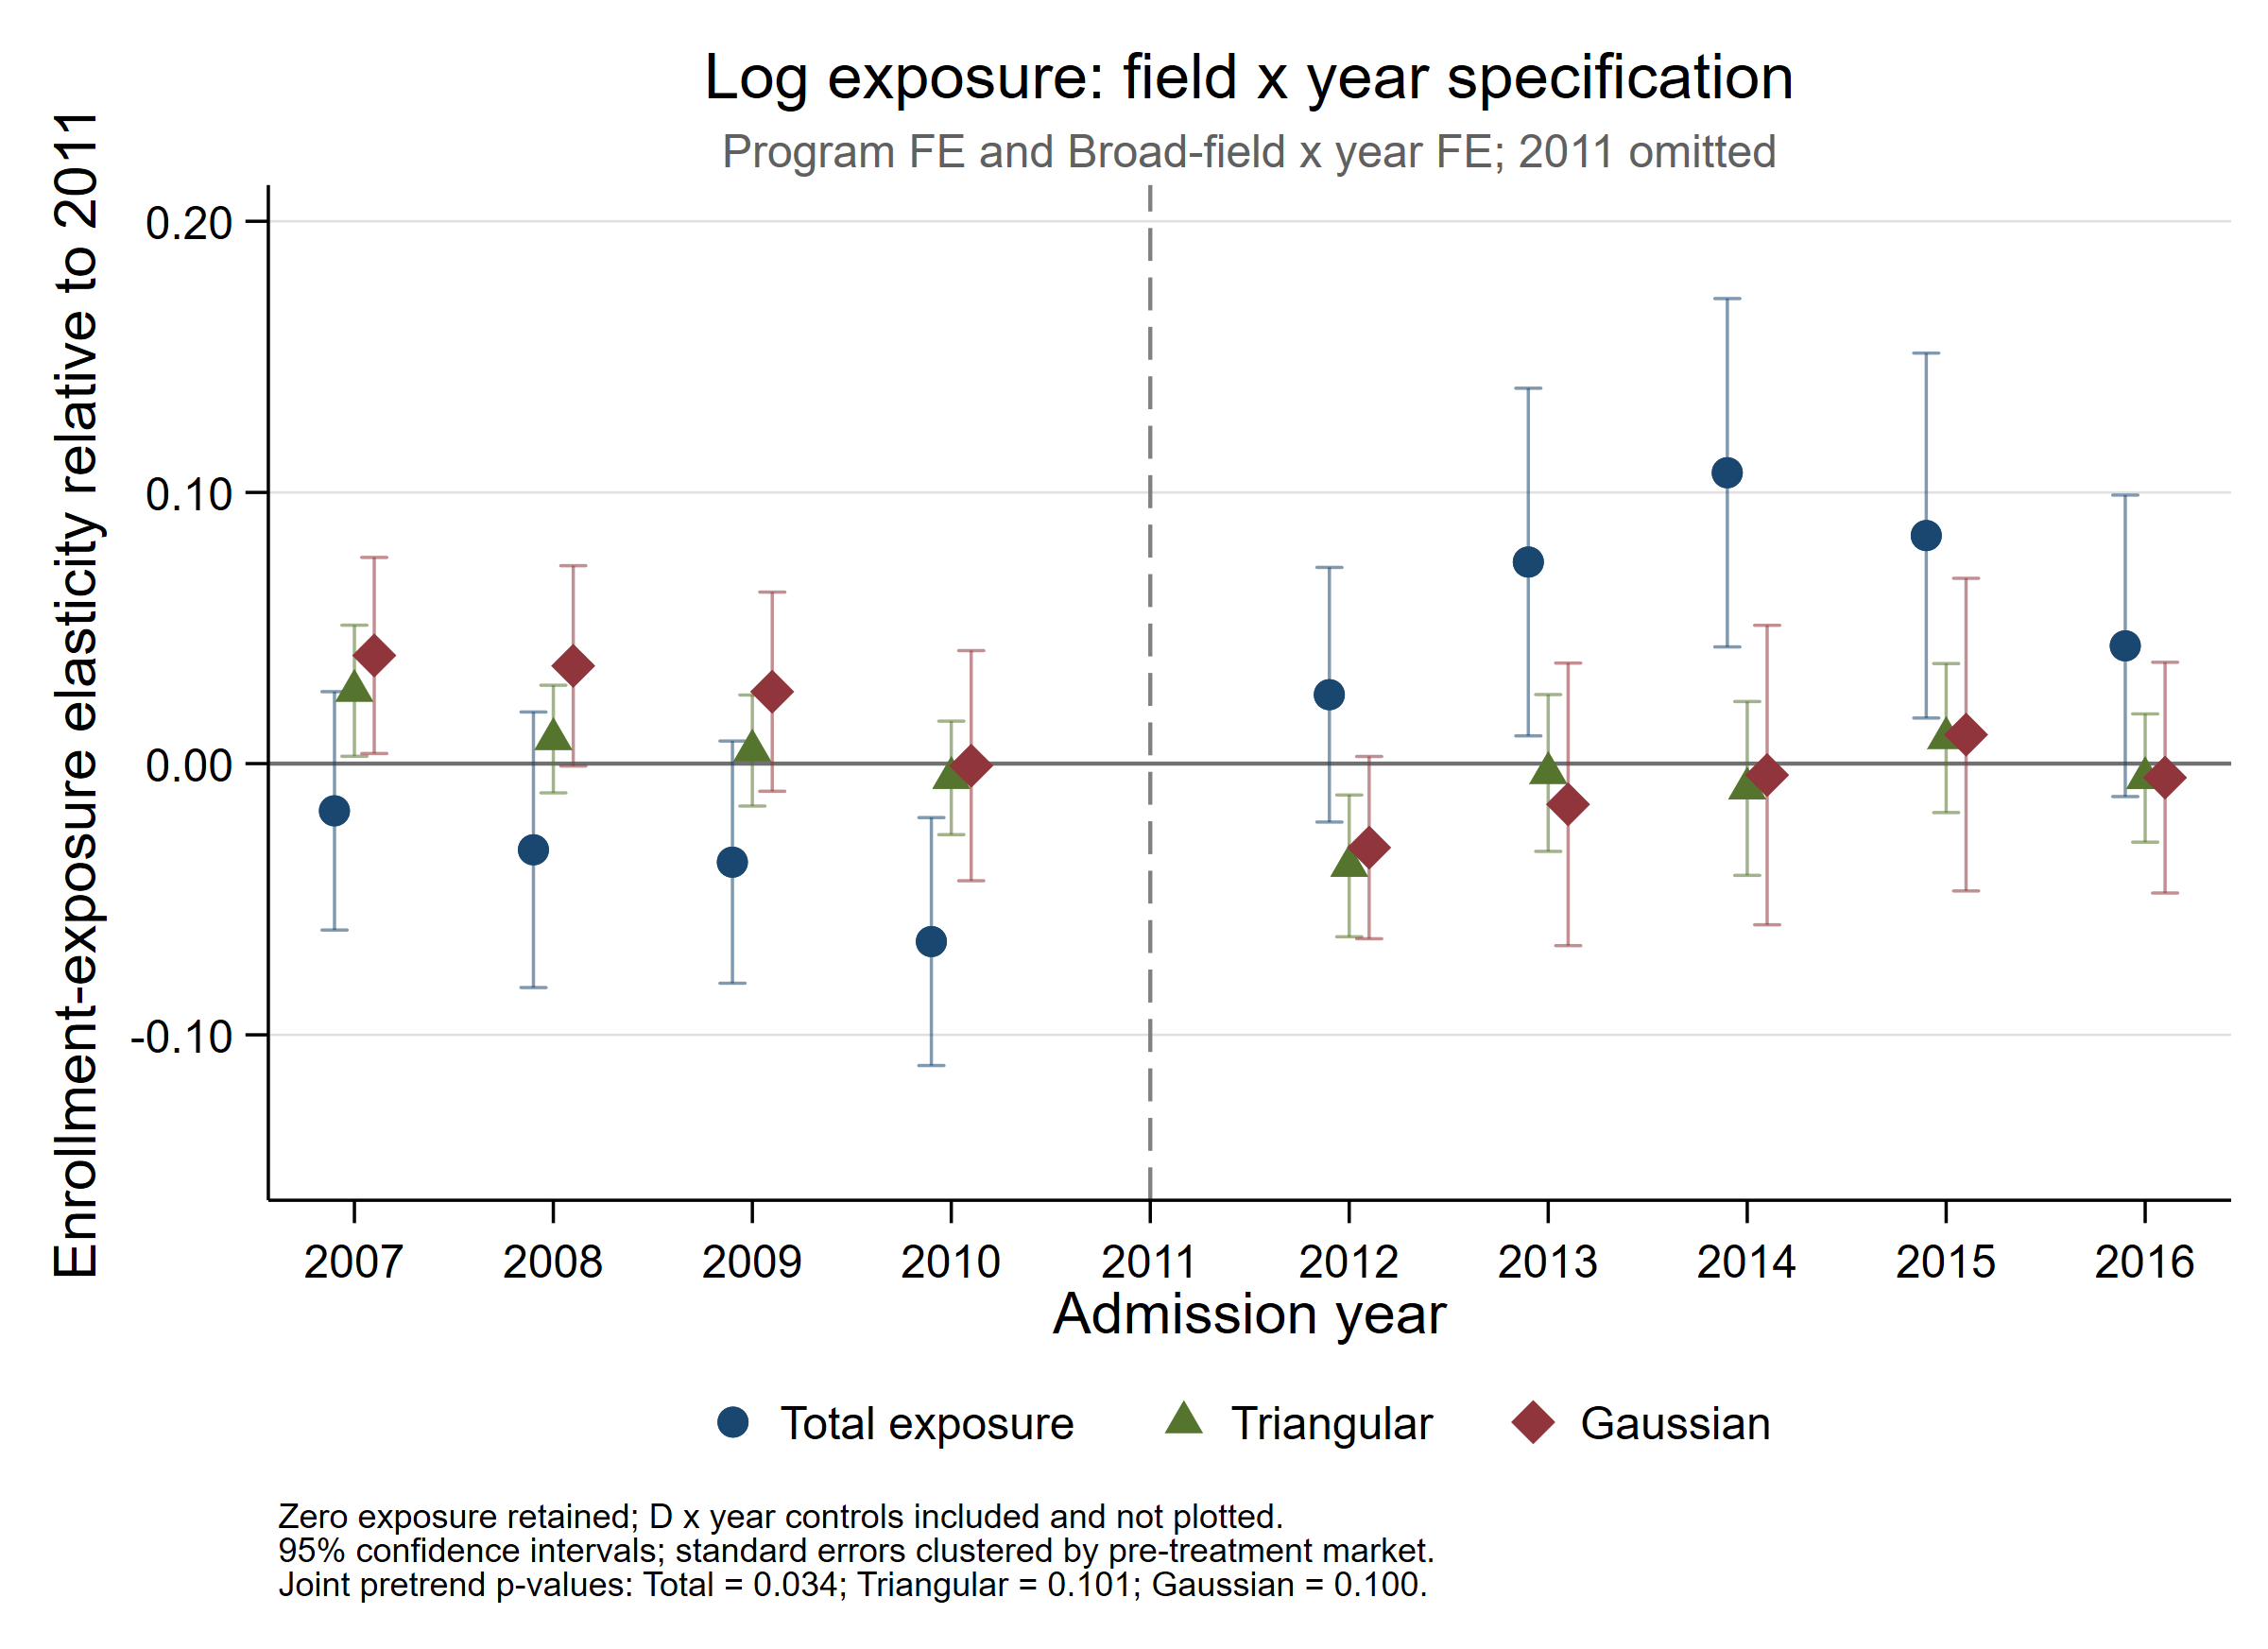
\includegraphics[ width=\linewidth ]{../../output/sua_log_event_study_baseline.png}
\end{column}

\begin{column}{0.495\textwidth}
    \centering

    \textbf{\scriptsize $+$ Region $\times$ year FE}

    \vspace{0.03cm}

    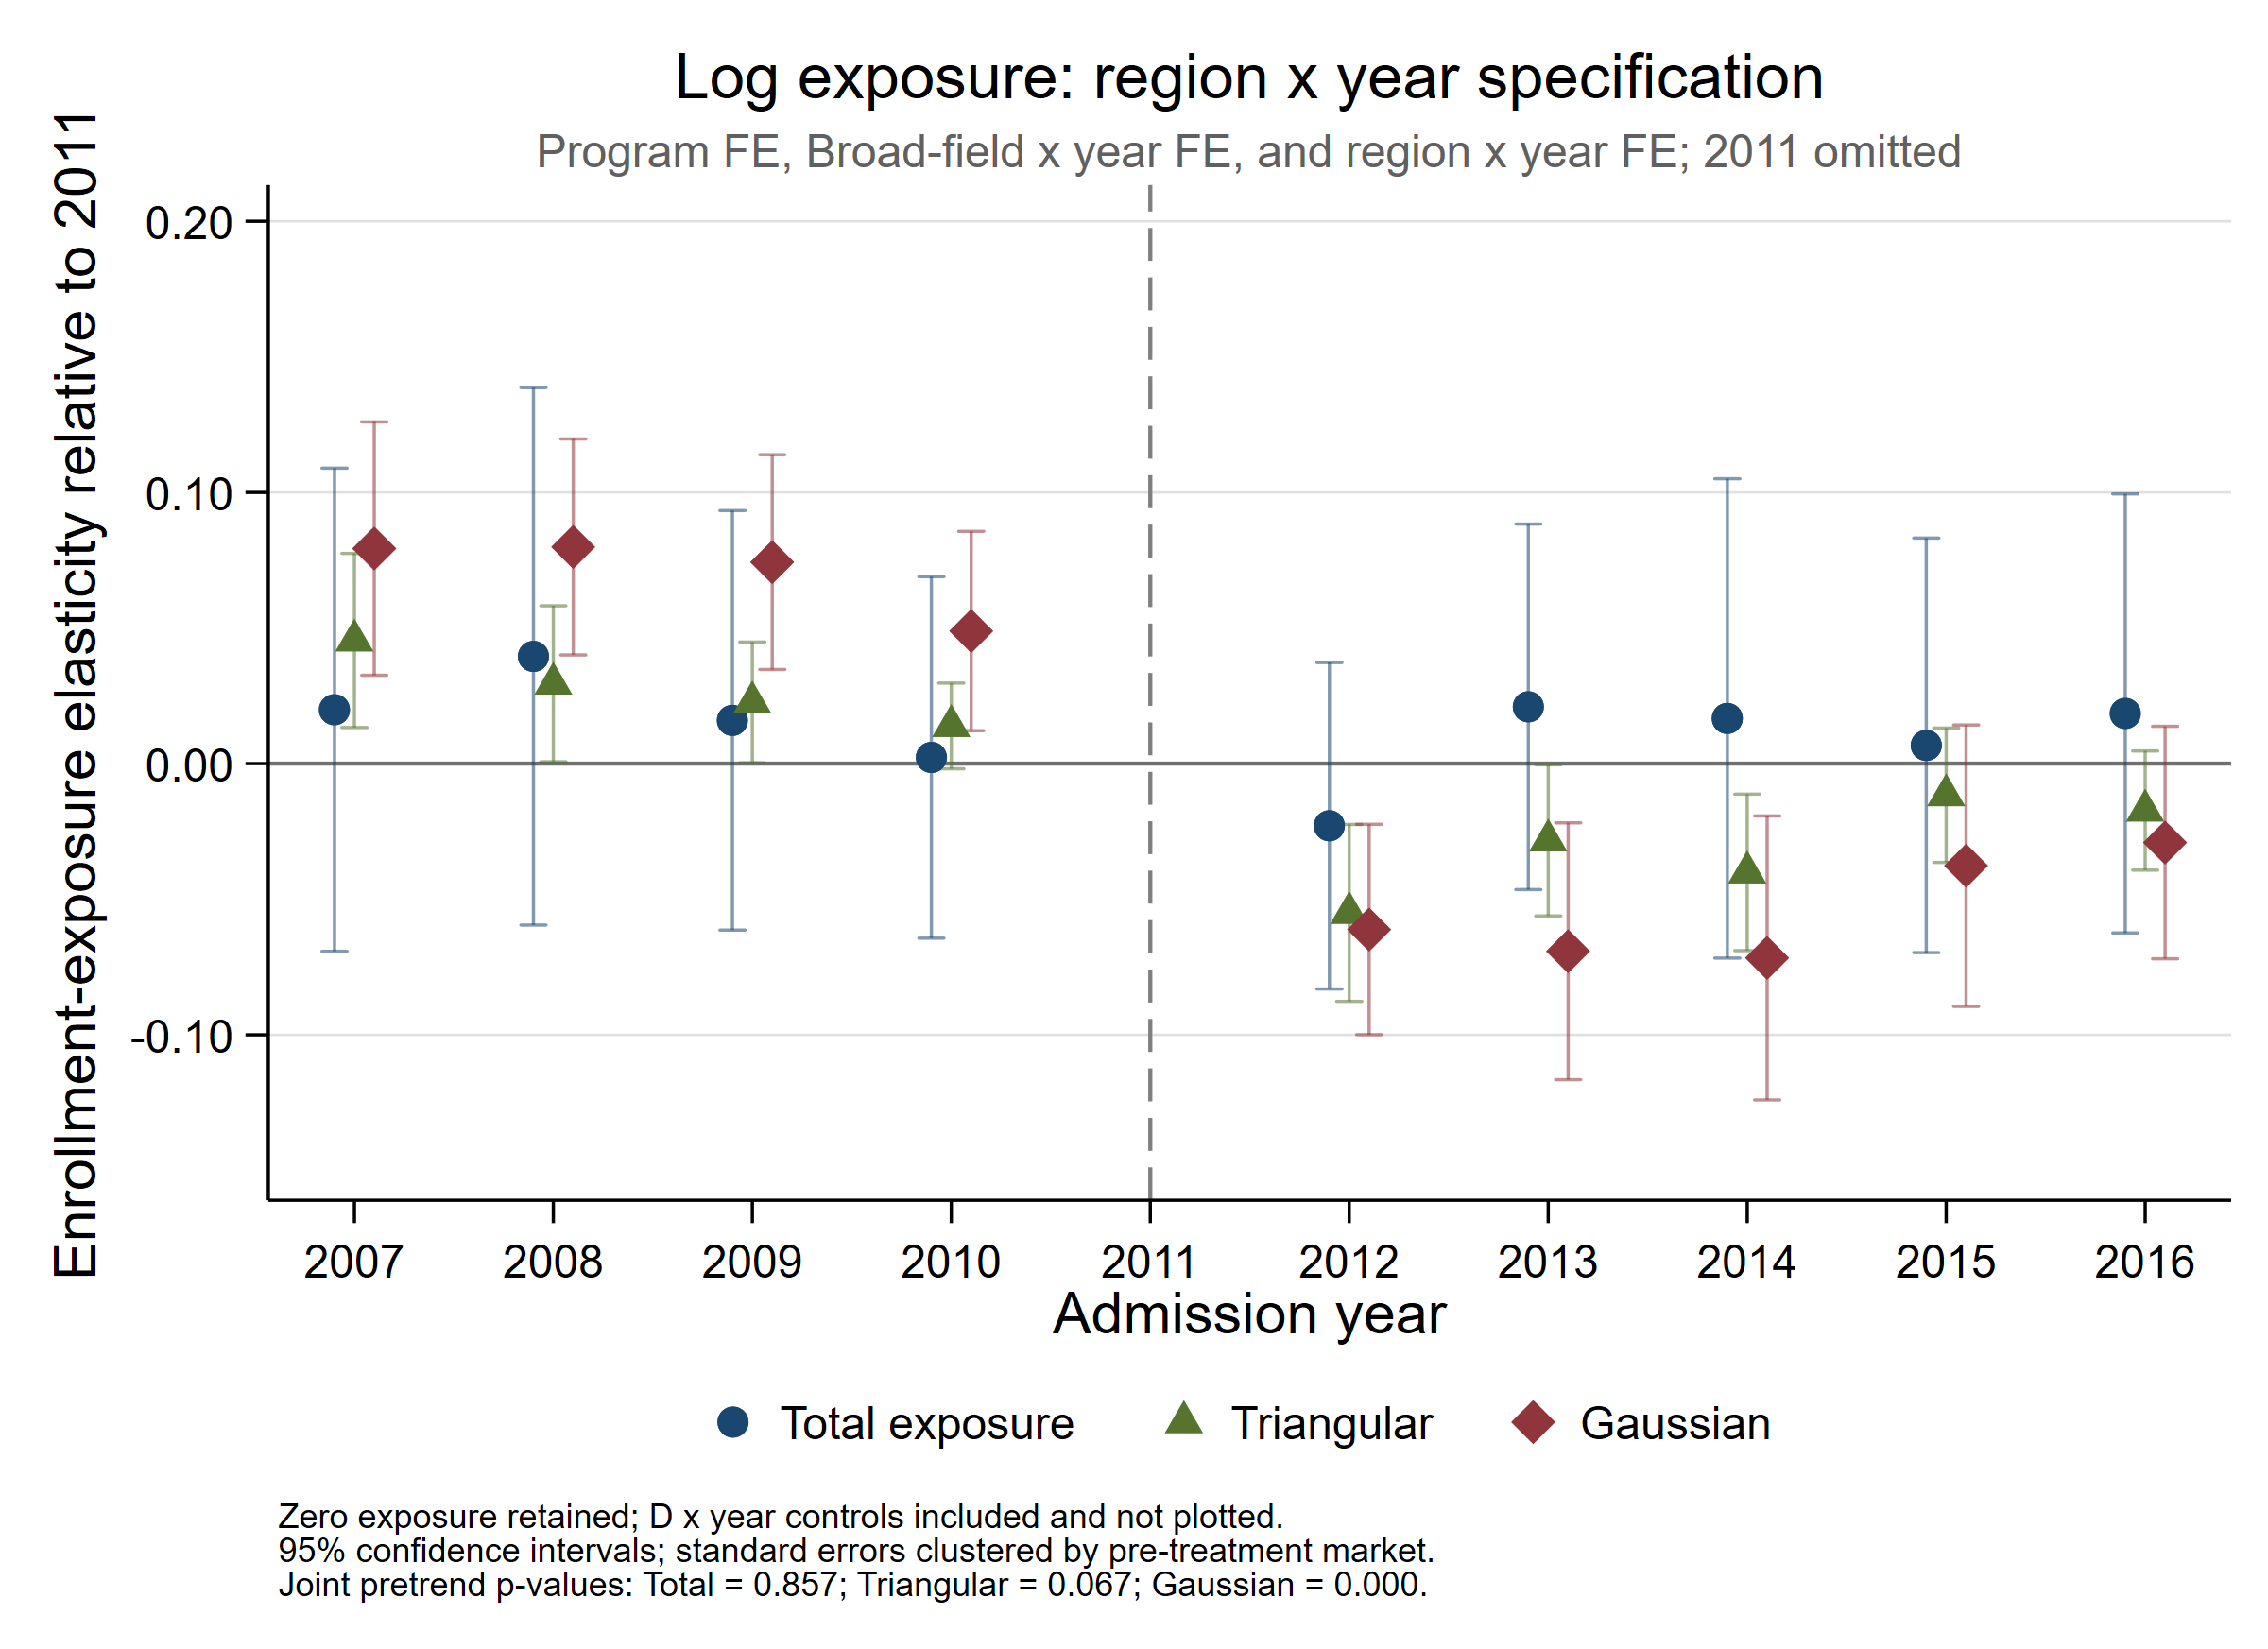
\includegraphics[ width=\linewidth ]{../../output/sua_log_event_study_regionyear.png}
\end{column}

\end{columns}

\vspace{-0.06cm}

\begin{center}
\begin{minipage}{0.97\textwidth}
\tiny
\textit{Notes:}
The figures use the Broad-field definition and report separate event studies
for Total, Triangular, and Gaussian exposure. The left panel absorbs program
and Broad-field $\times$ year fixed effects; the right panel additionally
absorbs pre-treatment region $\times$ year fixed effects. For each exposure
measure, zero-exposure programs are retained by setting
$\widetilde{\log E_p^k}=0$ when $E_p^k=0$ and including
$\mathbf{1}\{E_p^k>0\}\times\mathbf{1}\{t=s\}$ separately for every event year.
The plotted coefficients correspond to
$\widetilde{\log E_p^k}\times\mathbf{1}\{t=s\}$ and are interpreted relative
to 2011, the omitted year. Observations with zero first-year enrollment are
excluded because the dependent variable is in logs. Vertical bars report
95\% confidence intervals; standard errors are clustered by the
pre-treatment market. Joint tests of the 2007--2010 log-exposure coefficients
yield pretrend $p$-values of 0.034, 0.101, and 0.100 for Total, Triangular,
and Gaussian exposure in the left panel, and 0.857, 0.067, and 0.0001,
respectively, in the right panel.
\end{minipage}
\end{center}

\end{frame}

%---------------------------------------------------------
\begin{frame}[label=sua-kd-event-studies]

\frametitle{
    Event studies: kernel-weighted denominator
    \hfill
    \hyperlink{sua-kd-first-stage}{\scriptsize\color{blue}$\leftarrow$ First stage}
}

\vspace{-0.12cm}

\begin{columns}[T,onlytextwidth]
    \begin{column}{0.495\textwidth}
        \centering
        \textbf{\scriptsize Field $\times$ year FE}

        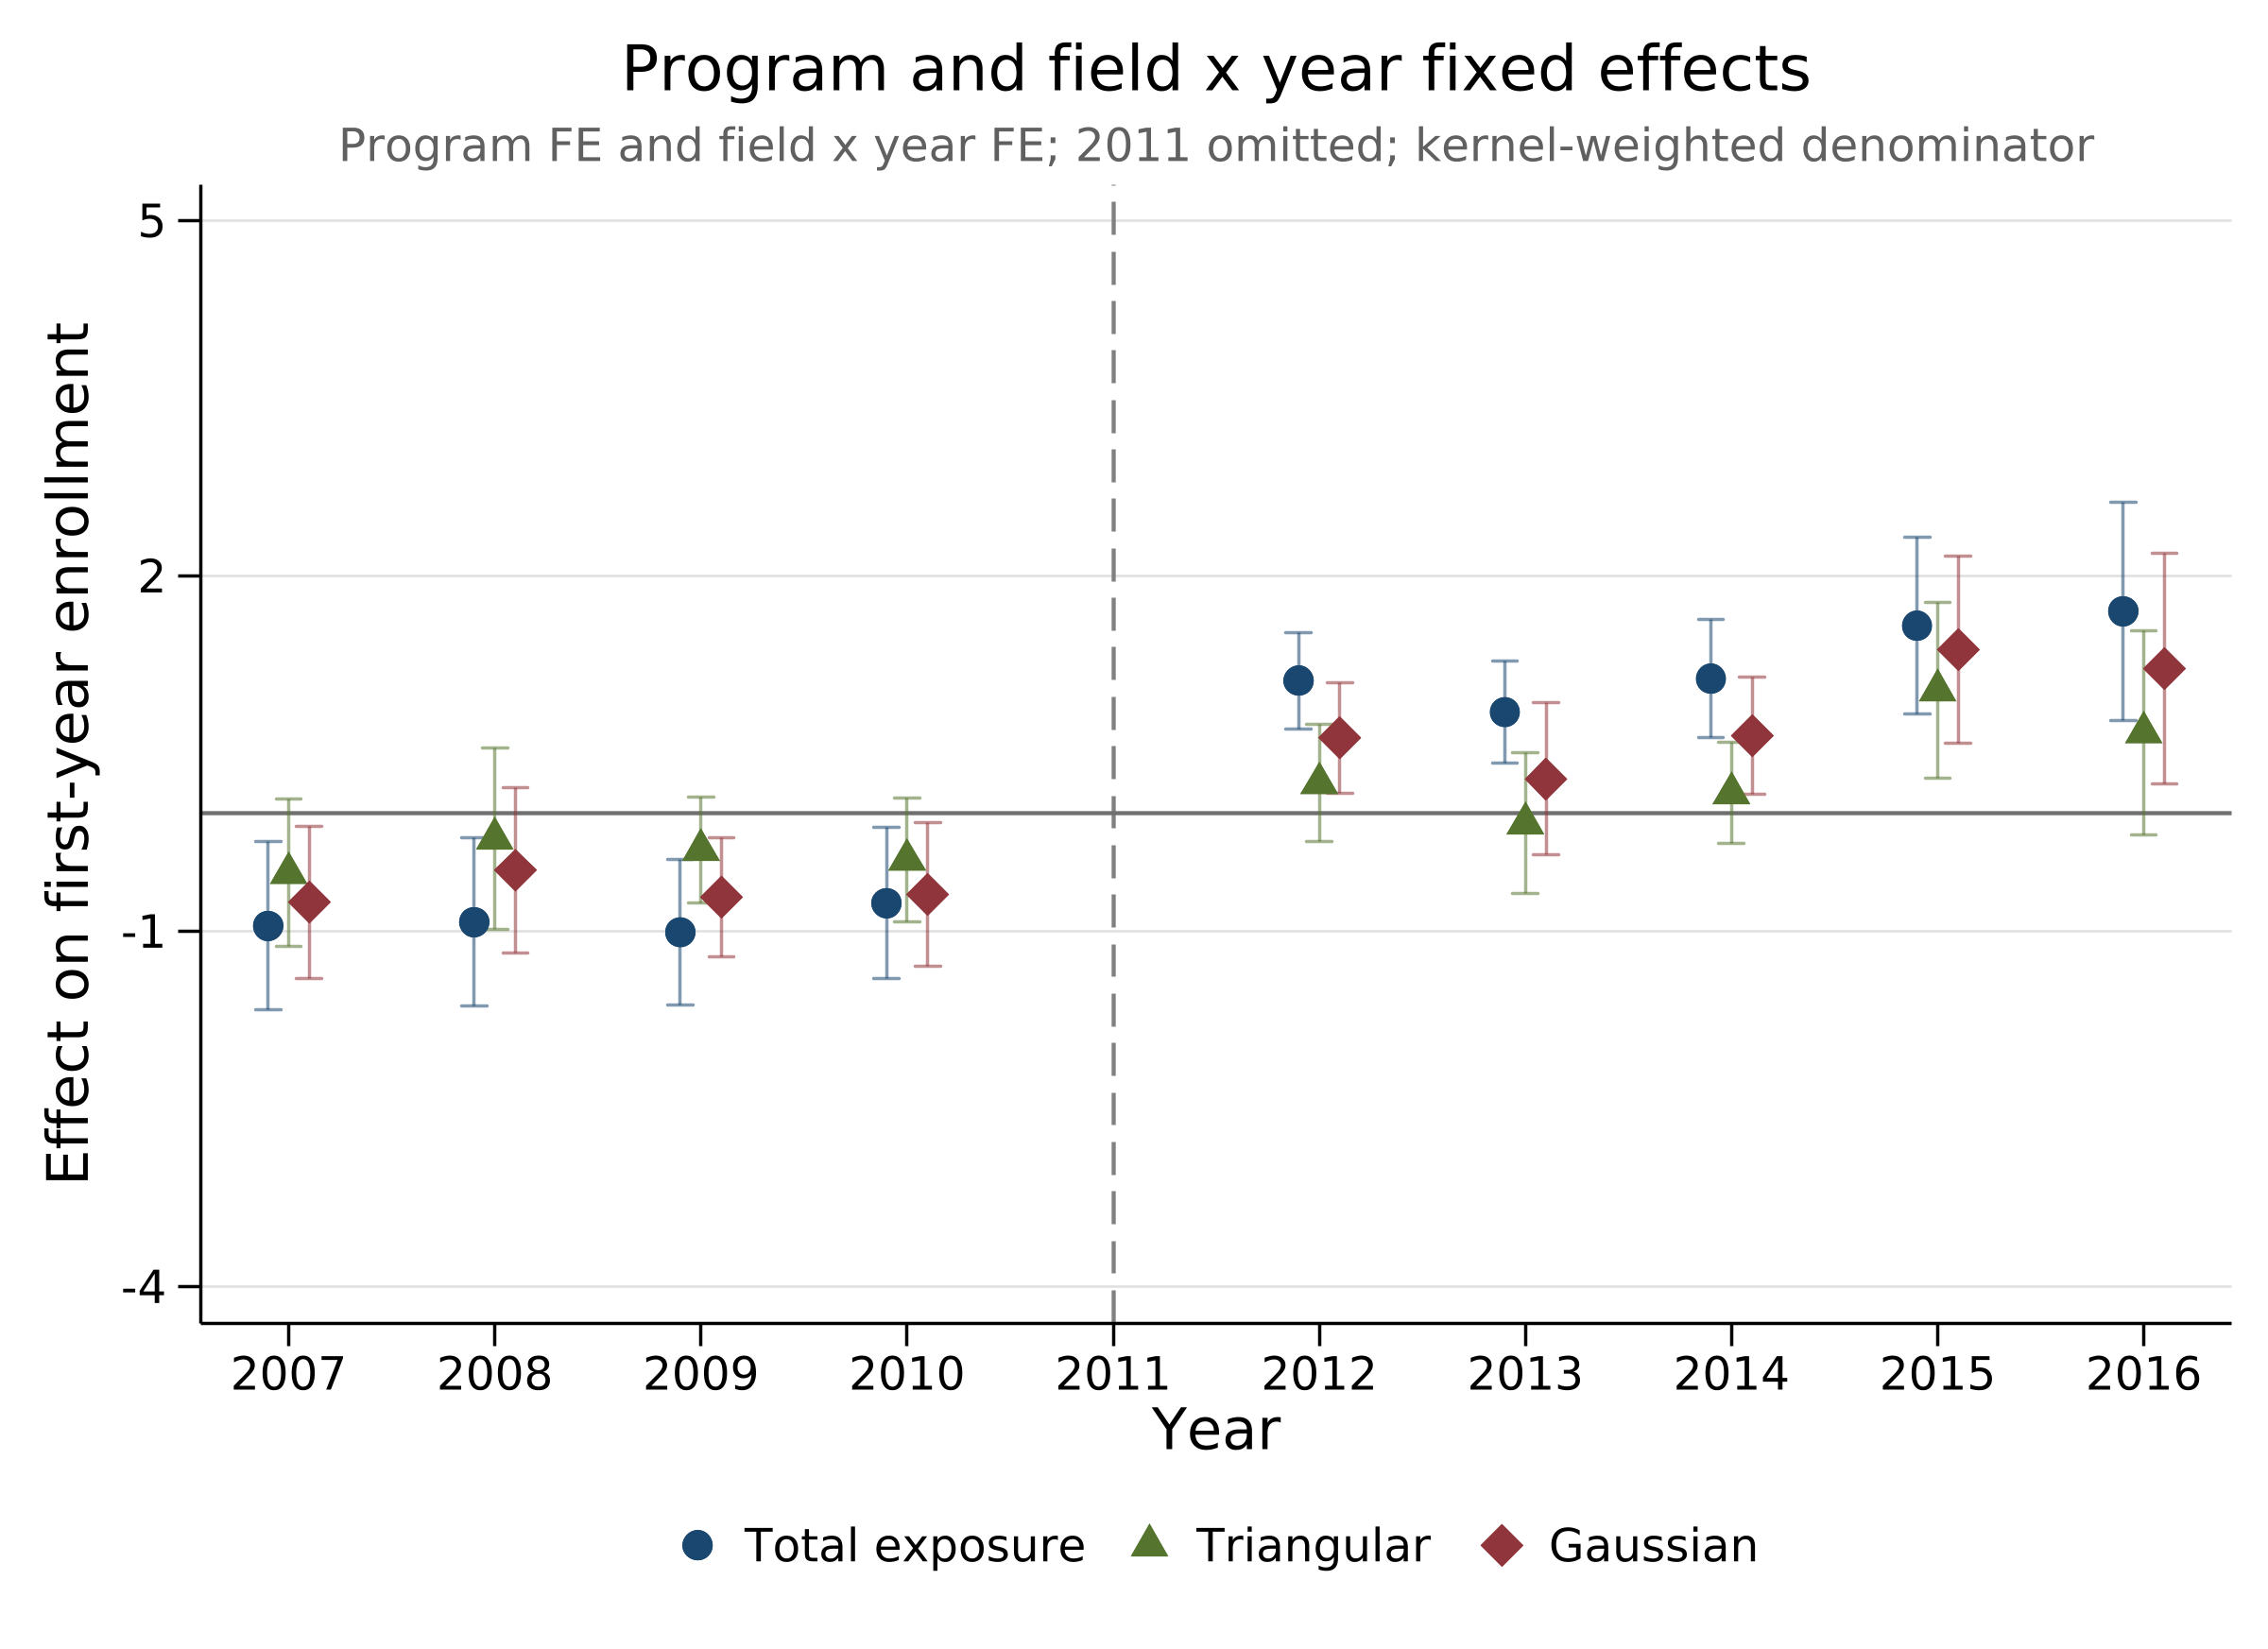
\includegraphics[width=\linewidth, height=0.66\textheight, keepaspectratio]{../../output/sua_event_study_exposure_comparison_baseline_kd.png}
    \end{column}
    \begin{column}{0.495\textwidth}
        \centering
        \textbf{\scriptsize $+$ Region $\times$ year FE}

        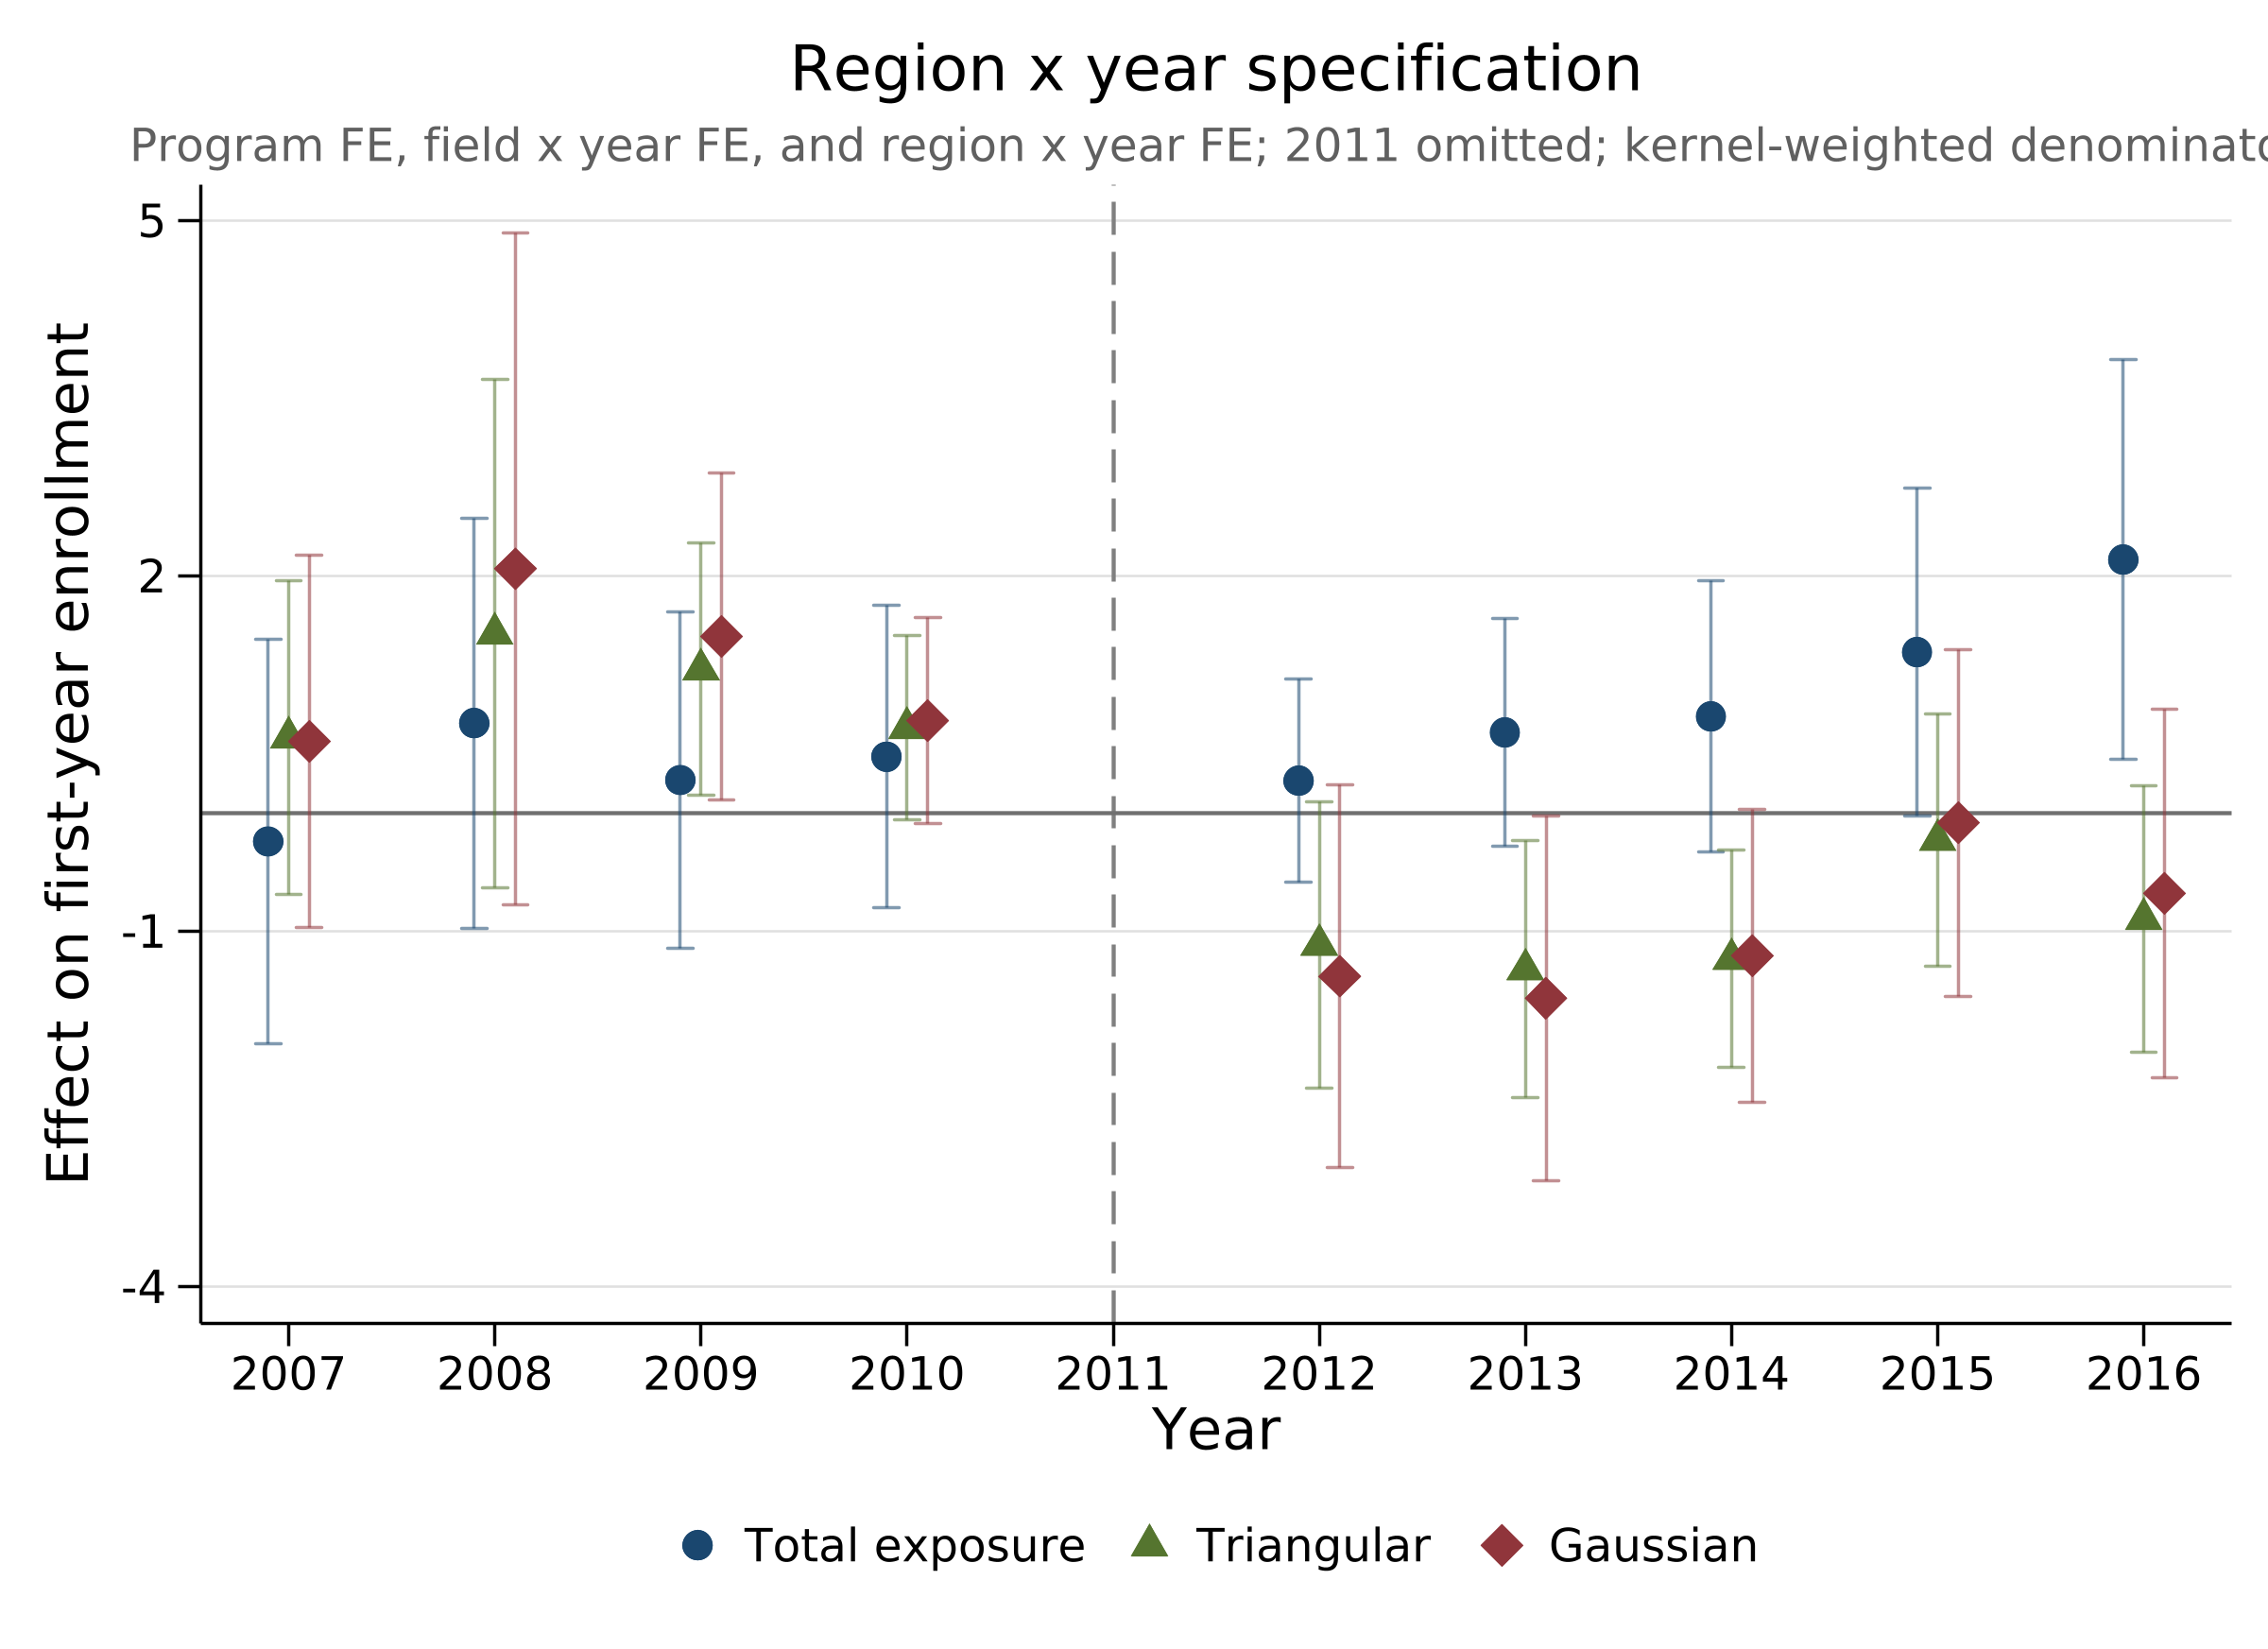
\includegraphics[width=\linewidth, height=0.66\textheight, keepaspectratio]{../../output/sua_event_study_exposure_comparison_regionyear_kd.png}
    \end{column}
\end{columns}

\vspace{0.04cm}

\begin{center}
\begin{minipage}{0.96\textwidth}
\tiny
\textit{Notes:}
Triangular and Gaussian exposure use the kernel-weighted denominator; Total
exposure is unchanged and shown for reference. Broad-field markets; separate
event studies for each measure. Coefficients measure the enrollment difference associated with a 10 percentage-point increase in exposure in each year relative to 2011. 95\% confidence intervals; SE clustered
by pre-treatment market. Joint pretrend $p$-values (2007--2010) for Total,
Triangular KD and Gaussian KD are 0.024, 0.170 and 0.022 in the left panel, and
0.285, 0.146 and 0.177 in the right panel.
\end{minipage}
\end{center}

\end{frame}

%---------------------------------------------------------
\begin{frame}[label=sua-kd-log-event-studies]

\frametitle{
    Log event studies: kernel-weighted denominator
    \hfill
    \hyperlink{sua-kd-log-first-stage}{\scriptsize\color{blue}$\leftarrow$ Log first stage}
}

\vspace{-0.12cm}

\begin{columns}[T,onlytextwidth]
    \begin{column}{0.495\textwidth}
        \centering
        \textbf{\scriptsize Field $\times$ year FE}

        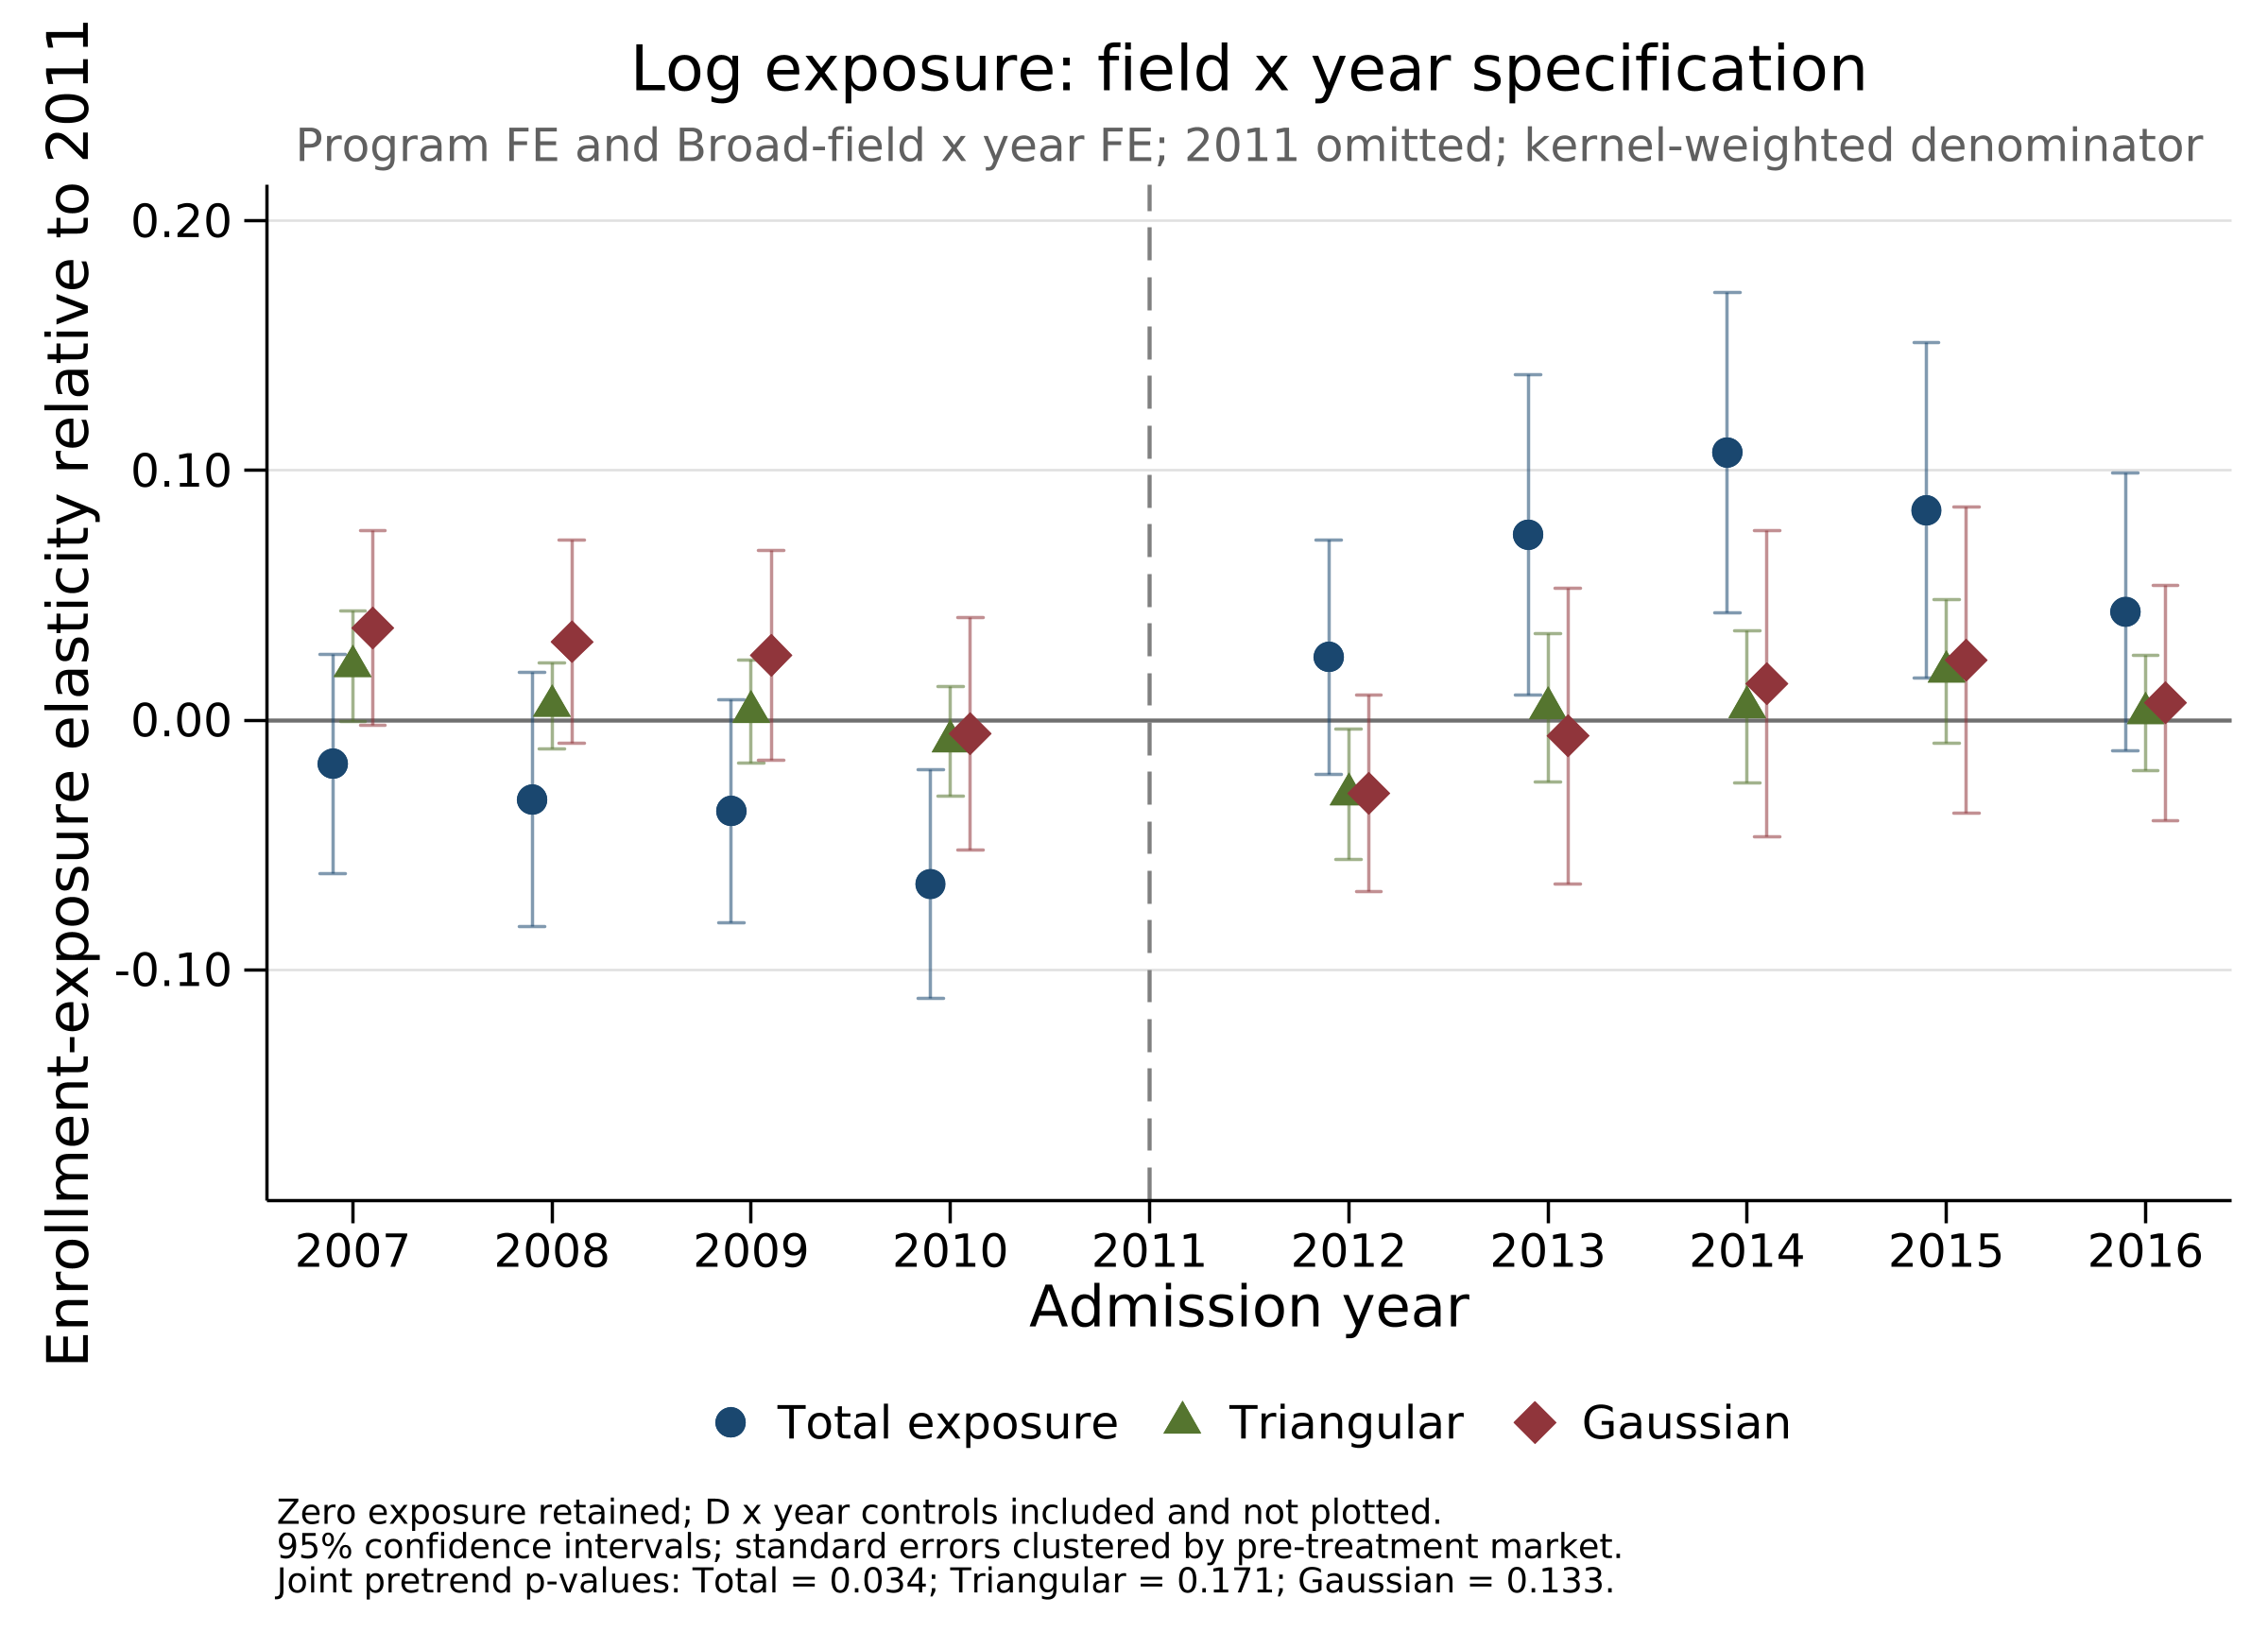
\includegraphics[width=\linewidth, height=0.66\textheight, keepaspectratio]{../../output/sua_log_event_study_baseline_kd.png}
    \end{column}
    \begin{column}{0.495\textwidth}
        \centering
        \textbf{\scriptsize $+$ Region $\times$ year FE}

        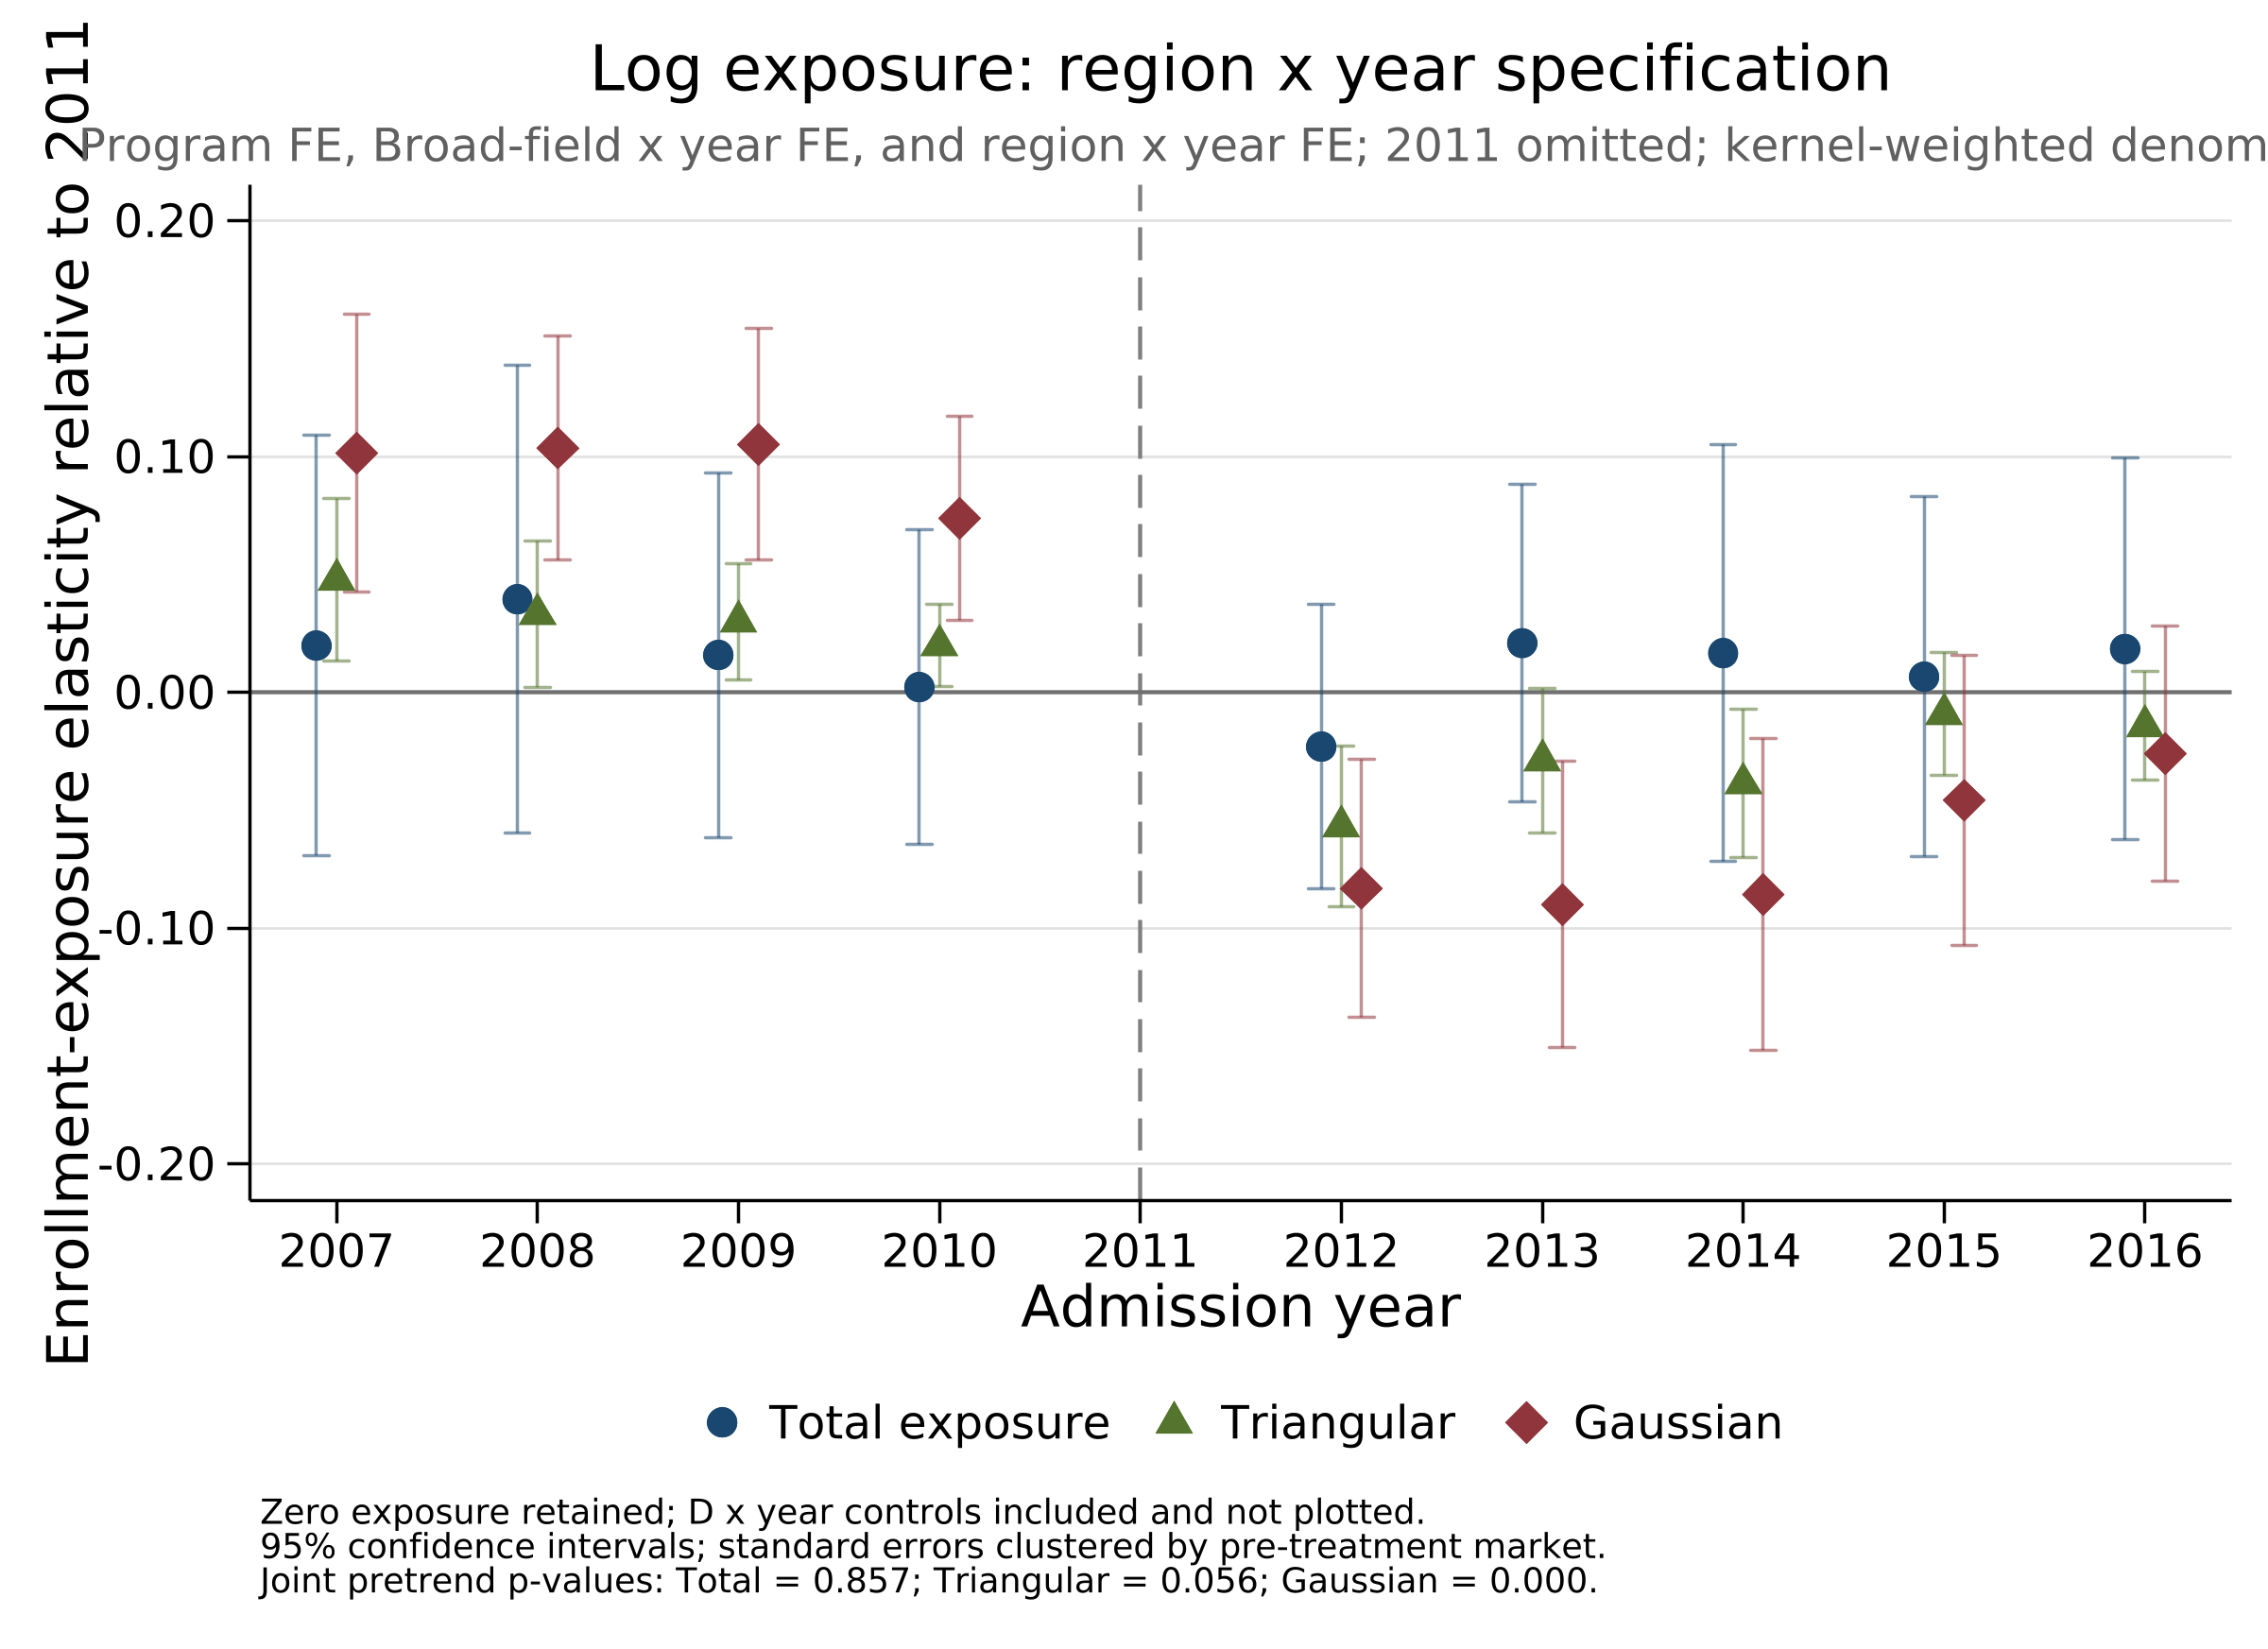
\includegraphics[width=\linewidth, height=0.66\textheight, keepaspectratio]{../../output/sua_log_event_study_regionyear_kd.png}
    \end{column}
\end{columns}

\vspace{0.04cm}

\begin{center}
\begin{minipage}{0.96\textwidth}
\tiny
\textit{Notes:}
Triangular and Gaussian exposure use the kernel-weighted denominator; Total
exposure is unchanged and shown for reference. Broad-field markets; separate
event studies for each measure. Plotted coefficients are those on the log-exposure $\times$ year terms, relative to 2011; $\mathbf{1}\{E>0\}\times$ year controls included. 95\% confidence intervals; SE clustered
by pre-treatment market. Joint pretrend $p$-values (2007--2010) for Total,
Triangular KD and Gaussian KD are 0.034, 0.171 and 0.133 in the left panel, and
0.857, 0.056 and 0.0001 in the right panel.
\end{minipage}
\end{center}

\end{frame}

%---------------------------------------------------------
\begin{frame}{Decomposing weighted exposure}

\scriptsize
\setlength{\abovedisplayskip}{3pt}
\setlength{\belowdisplayskip}{3pt}

%---------------------------------------------------------
% ORIGINAL EXPOSURE AND EXACT DECOMPOSITION
%---------------------------------------------------------
\begin{center}
\resizebox{0.75\textwidth}{!}{
$
\displaystyle
\underbrace{
E_p^k
=
\frac{
\sum_{q\in\mathcal E_{m(p)}}
k\!\left(|S_p-S_q|\right)N_q
}{
\sum_{\ell\in m(p)}N_\ell
}
}_{\substack{
\text{Direct construction}\\
\text{of weighted exposure}
}}
\quad\equiv\quad
\begin{gathered}
E_p^k
=
\left[
\frac{
\sum_{q\in\mathcal E_{m(p)}}N_q
}{
\sum_{\ell\in m(p)}N_\ell
}
\right]
\left[
\frac{
\sum_{q\in\mathcal E_{m(p)}}
k\!\left(|S_p-S_q|\right)N_q
}{
\sum_{q\in\mathcal E_{m(p)}}N_q
}
\right]
\\[0.18cm]
E_p^k
=
\underbrace{
M_{m(p)}
}_{\substack{
\text{entrant}\\
\text{market share}
}}
\;\times\;
\underbrace{
Q_p^k
}_{\substack{
\text{similarity}\\
\text{with entrants}
}}
\end{gathered}
$
}
\end{center}

\vspace{0.05cm}

%---------------------------------------------------------
% COMPONENTS OF THE DECOMPOSITION
%---------------------------------------------------------

\begin{columns}[T,onlytextwidth]

\begin{column}{0.47\textwidth}

\textbf{Entrant presence}

\tiny
\[
M_m
=
\frac{
\sum_{q\in\mathcal E_m}N_q
}{
\sum_{\ell\in m}N_\ell
}.
\]

\tiny
\(M_m\) is the entrant share of total market enrollment. It captures the
\textbf{size of entrant presence} and is common to all incumbent programs
in market \(m\).

\end{column}

\begin{column}{0.50\textwidth}

\textbf{Conditional similarity}

\tiny
\[
Q_p^k
=
\frac{
\sum_{q\in\mathcal E_m}
k\!\left(|S_p-S_q|\right)N_q
}{
\sum_{q\in\mathcal E_m}N_q
}.
\]

\tiny
\(Q_p^k\) is the entrant-enrollment-weighted PSU similarity between incumbent
\(p\) and the entrant programs in its market. It is higher when larger
entrants have PSU profiles closer to that of \(p\).
Conditional on entrant presence, it captures \textbf{competitive proximity}
rather than the overall size of entry.

\end{column}

\end{columns}

\vspace{0.06cm}

%---------------------------------------------------------
% FIRST STAGE USING Q
%---------------------------------------------------------

\textbf{Using similarity as the independent variable}

\tiny
\[
N^{\mathrm{first}}_{pt}
=
\beta_k
\left[
Q_p^k\times Post_t
\right]
+\mu_p+\alpha_{f(p),t}+\gamma_{r(p),t}
+\varepsilon_{pt},
\qquad M_{m(p)}>0.
\]

\tiny
The sample is restricted to markets with positive entrant presence.
Program fixed effects absorb time-invariant differences across incumbents,
while Broad-field \(\times\) year and pre-treatment region \(\times\) year
fixed effects absorb common field-specific and regional shocks over time.
The model therefore asks whether, among incumbents in exposed markets,
programs whose pre-treatment PSU profiles are more similar to the entrants
experience different post-2012 enrollment changes.
Unlike \(E_p^k\), which combines entrant market share and similarity,
\(Q_p^k\) isolates the \textbf{similarity component} of exposure.
The coefficient \(\beta_k\) measures the differential post-2012 enrollment
change associated with a 0.10 increase in entrant-enrollment-weighted PSU
similarity.

\end{frame}

%---------------------------------------------------------
\begin{frame}[label=sua-q-main]

\frametitle{Distribution of conditional similarity measures}

\centering

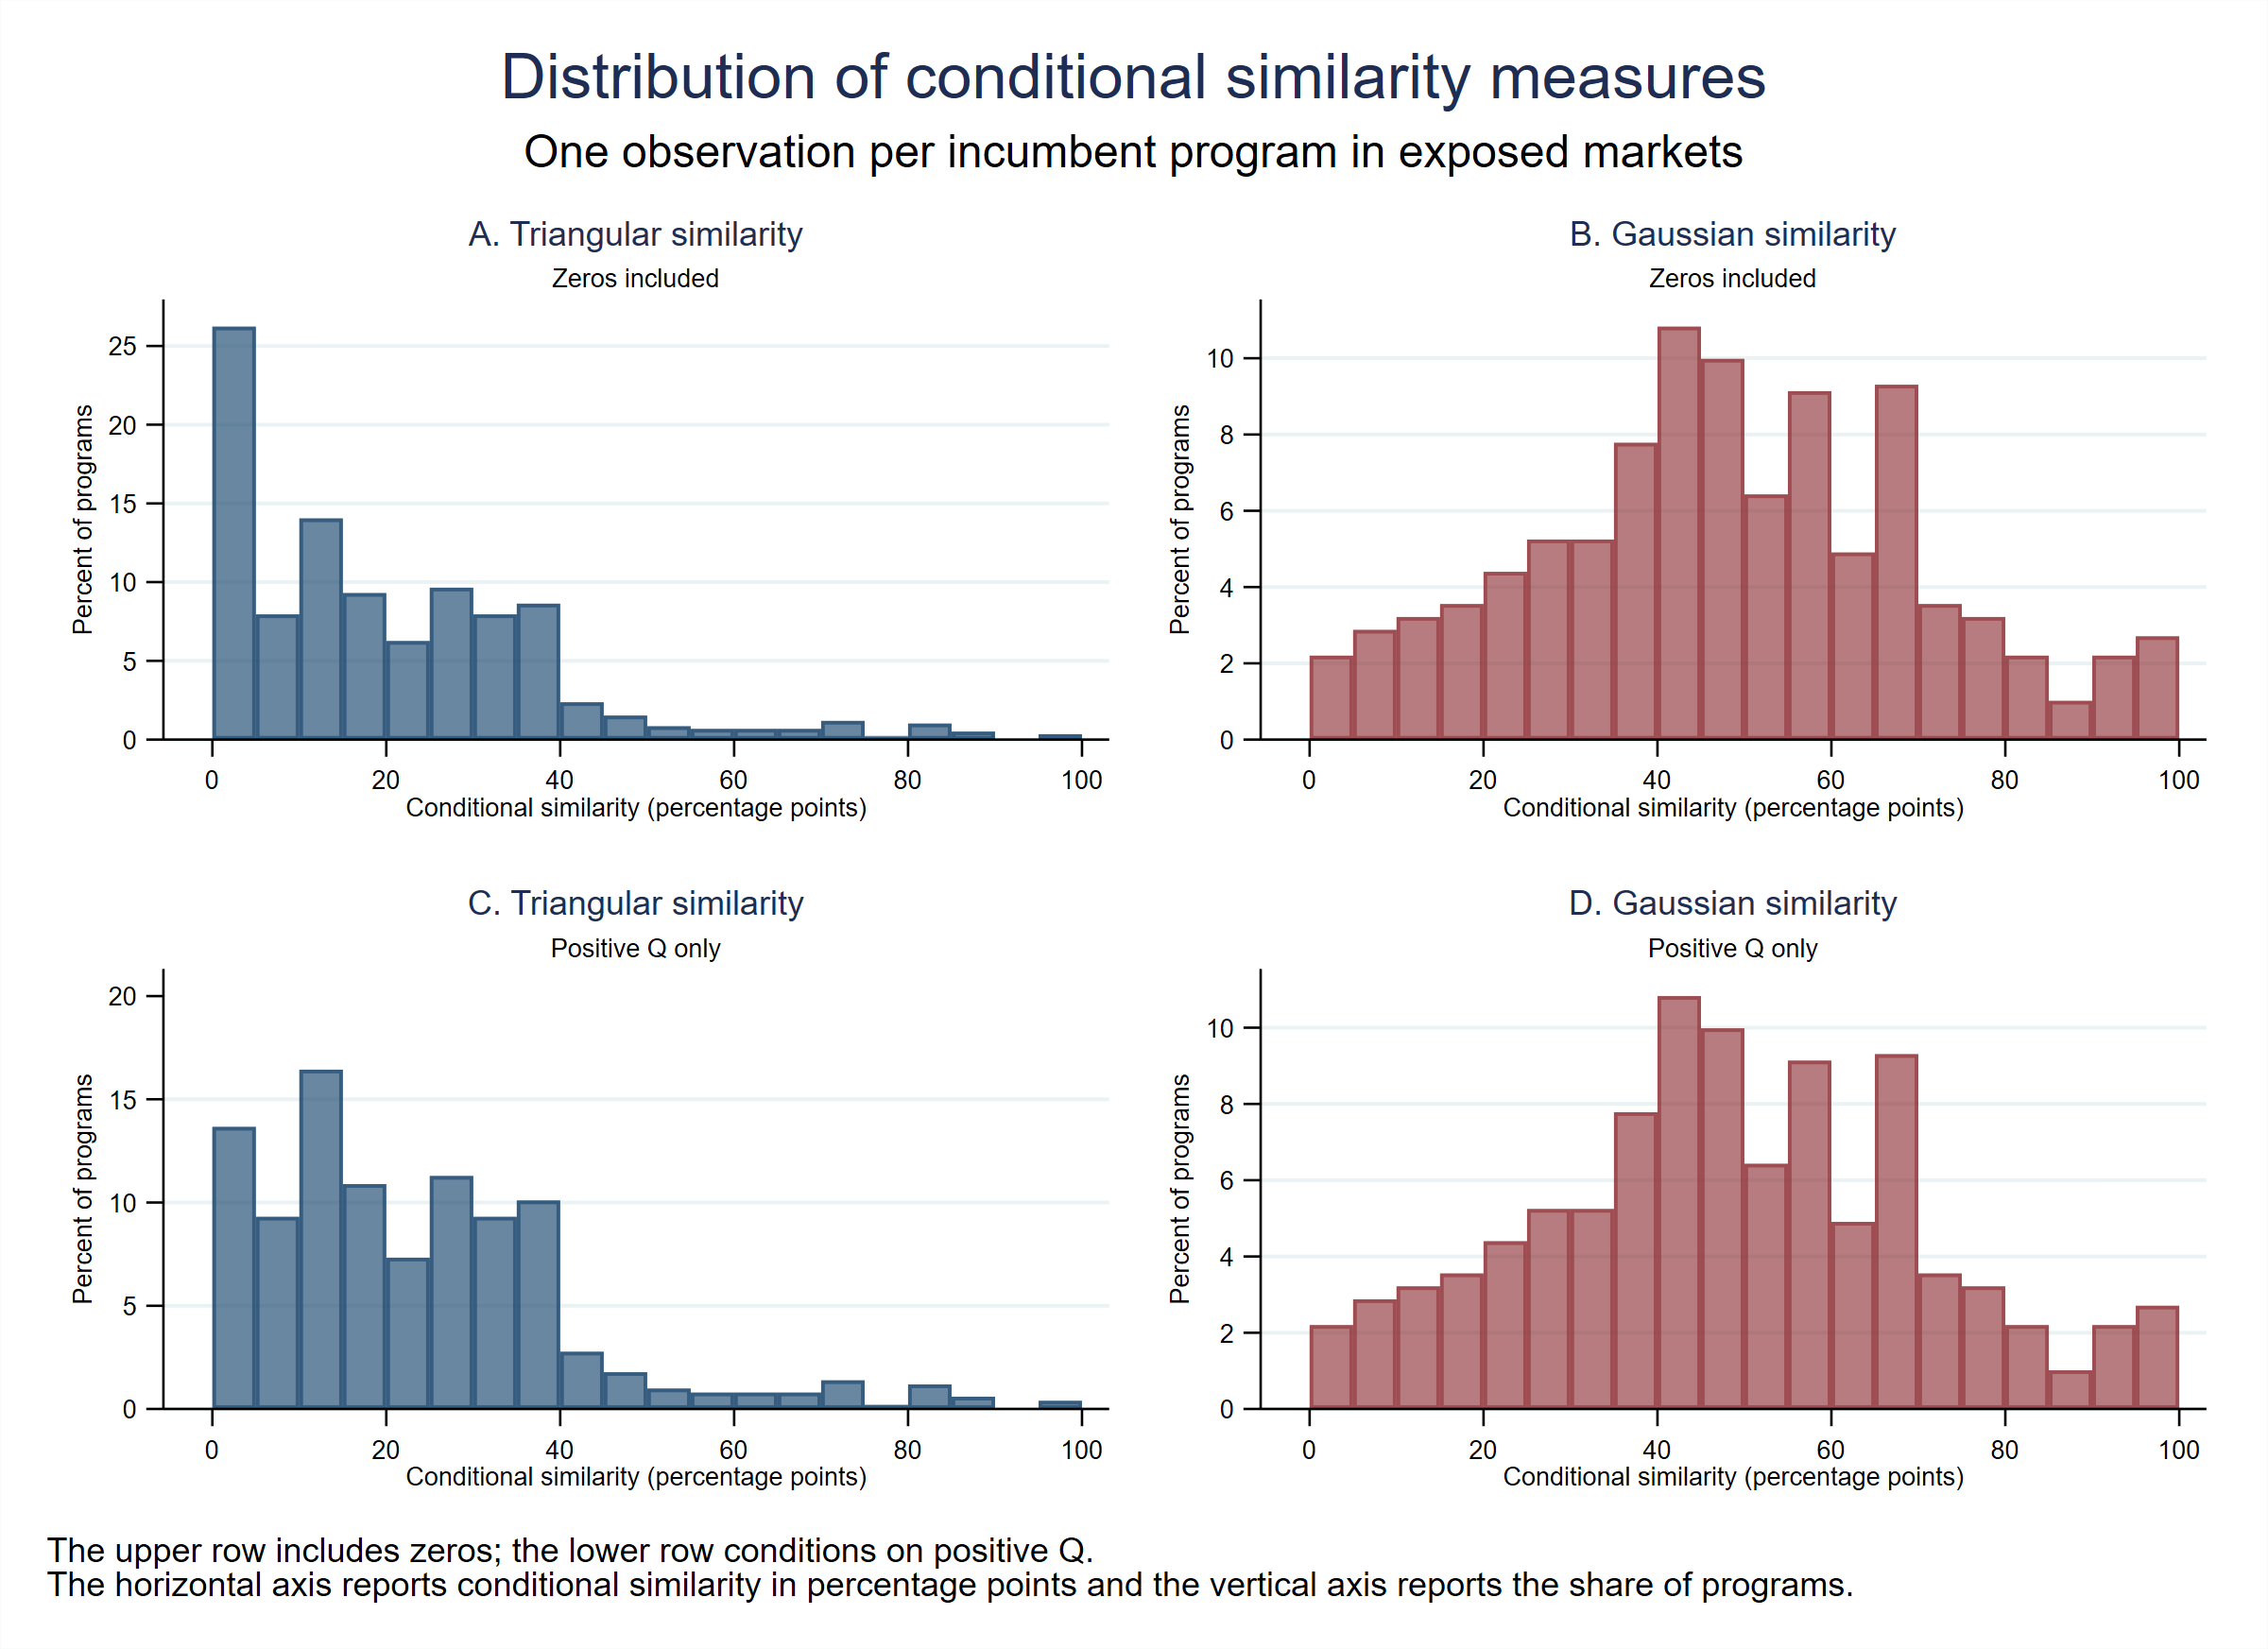
\includegraphics[ width=0.84\textwidth, height=0.64\textheight, keepaspectratio ]{../../output/sua_q_distributions_combined.png}

\vspace{-0.10cm}


\begin{itemize}
\tiny  
\setlength{\itemsep}{2pt}

\item Each incumbent program appears once. The horizontal axis reports
conditional similarity $Q$ in percentage points and the vertical axis
the share of programs.

\item The upper row includes all exposed programs, while the lower row
excludes zeros and shows the distribution conditional on positive $Q$.

\item Triangular similarity is concentrated at relatively low values and
contains a relevant mass near zero. Gaussian similarity is more
dispersed and shifted toward higher values, indicating a less restrictive
measure of similarity across exposed markets.

\end{itemize}

\end{frame}

%---------------------------------------------------------
\begin{frame}[label=sua-similarity-first-stage]

\frametitle{
Similarity within exposed markets
\hfill
\hyperlink{sua-similarity-event-studies}{
\scriptsize\color{blue}
Event studies $\rightarrow$
}
}

\scriptsize
\setlength{\abovedisplayskip}{3pt}
\setlength{\belowdisplayskip}{3pt}

\textbf{Common fixed-effects specification}


\begin{center}
\resizebox{1\textwidth}{!}{
$
\begin{gathered}
\begin{aligned}
N^{\mathrm{first}}_{pt}
&=
\beta_k
\left[
Q_p^k\times Post_t
\right]
+\mu_p+\alpha_{f(p),t}
+\gamma_{r(p),t}
+\varepsilon_{pt},
\end{aligned}
\qquad
\begin{aligned}
\log N^{\mathrm{first}}_{pt}
&=
\delta_k
\left[
\widetilde{\log Q_p^k}\times Post_t
\right]
+
\theta_k
\left[
D_p^k\times Post_t
\right]
+\mu_p+\alpha_{f(p),t}
+\gamma_{r(p),t}
+\varepsilon_{pt},
\end{aligned}
\\[-0.02cm]
\widetilde{\log Q_p^k}
=
\begin{cases}
\log(Q_p^k), & Q_p^k>0,\\
0, & Q_p^k=0,
\end{cases}
\qquad
D_p^k=\mathbf{1}\{Q_p^k>0\},
\qquad
M_m>0.
\end{gathered}
$
}
\end{center}

\vspace{0.06cm}

\begin{table}
\centering
\tiny
\setlength{\tabcolsep}{5pt}
\renewcommand{\arraystretch}{1.05}

\resizebox{0.70\textwidth}{!}{
\begin{tabular}{lcccc}
\toprule
&
\multicolumn{2}{c}{Levels}
&
\multicolumn{2}{c}{Logs}
\\
\cmidrule(lr){2-3}
\cmidrule(lr){4-5}

&
Triangular
&
Gaussian
&
Triangular
&
Gaussian
\\
\midrule

Similarity term $\times$ Post
& $-2.381^{***}$
& $-2.241^{***}$
& $-0.067^{***}$
& $-0.142^{***}$
\\

&
$(0.491)$
&
$(0.487)$
&
$(0.020)$
&
$(0.035)$
\\

Wald $F$
& 23.50
& 21.18
& 11.37
& 16.29
\\

Observations
& 5,009
& 5,009
& 5,009
& 5,009
\\

Programs
& 591
& 591
& 591
& 591
\\

Markets
& 36
& 36
& 36
& 36
\\

\bottomrule
\end{tabular}
}

\vspace{0.08cm}

\parbox{0.94\textwidth}{
\tiny
\textit{Notes:}
In levels, a 0.10 increase in conditional similarity is associated with
approximately 2.2--2.4 fewer first-year students after 2012.
In logs, a 10\% increase in similarity is associated with approximately
0.67\% lower enrollment under the triangular measure and 1.42\% lower
enrollment under the Gaussian measure.
The sample is restricted to markets with positive entrant presence,
$M_m>0$. Levels retain economically meaningful observations with $Q_p^k=0$.
In logs, zero-similarity observations are also retained by setting
$\widetilde{\log Q_p^k}=0$ when $Q_p^k=0$ and including
$D_p^k\times Post_t$ separately. The coefficient on this indicator is not
reported. Gaussian similarity is strictly positive in the exposed-market
sample, so the corresponding indicator is absorbed by the fixed effects.
All regressions absorb program, Broad-field $\times$ year, and
pre-treatment region $\times$ year fixed effects.
Standard errors clustered by pre-treatment market are in parentheses.
Event studies reject the absence of differential pre-treatment trends,
so estimates are interpreted as descriptive rather than causal.
$^{***}p<0.01$.
}

\end{table}

\end{frame}

%---------------------------------------------------------
\begin{frame}[label=sua-q-heterogeneity]

\frametitle{Conditional similarity: heterogeneity by incumbent selectivity}

\centering

\begin{table}
\centering
\tiny
\setlength{\tabcolsep}{4.5pt}
\renewcommand{\arraystretch}{0.95}

\begin{tabular}{lcccccc}
\toprule
& \multicolumn{2}{c}{PSU $<550$}
& \multicolumn{2}{c}{PSU $550$--$649$}
& \multicolumn{2}{c}{PSU $\geq650$} \\
\cmidrule(lr){2-3}
\cmidrule(lr){4-5}
\cmidrule(lr){6-7}
& Tri.
& Gau.
& Tri.
& Gau.
& Tri.
& Gau. \\
\midrule

\multicolumn{7}{l}{\textit{Conditional similarity $Q$}} \\[2pt]

Coefficient
& $-1.95^{*}$
& $-3.26$
& $-2.20^{***}$
& $-2.17^{***}$
& $-5.70$
& $-3.48$ \\

& $(0.93)$
& $(1.96)$
& $(0.48)$
& $(0.37)$
& $(4.24)$
& $(3.15)$ \\

$F$-statistic
& 4.40
& 2.77
& 21.27
& 34.14
& 1.80
& 1.22 \\


Observations
& \multicolumn{2}{c}{836}
& \multicolumn{2}{c}{2,932}
& \multicolumn{2}{c}{1,038} \\

Programs
& \multicolumn{2}{c}{104}
& \multicolumn{2}{c}{339}
& \multicolumn{2}{c}{128} \\

Clusters
& \multicolumn{2}{c}{15}
& \multicolumn{2}{c}{28}
& \multicolumn{2}{c}{16} \\

\bottomrule
\end{tabular}
\end{table}

\vspace{-0.05cm}

\parbox{0.95\textwidth}{
\tiny
\textit{Notes:}
Standard errors clustered by pre-treatment market in parentheses.
All regressions include program and market$\times$year FE and are restricted
to exposed markets. Coefficients correspond to a 0.10 increase in conditional
similarity. The same split for SUA exposure is in the
\hyperlink{sua-selectivity-heterogeneity}{\color{blue}main text}.
$^{*}p<0.10$, $^{**}p<0.05$, $^{***}p<0.01$.
}

\end{frame}

%---------------------------------------------------------
\begin{frame}[label=sua-similarity-event-studies]

\frametitle{
Similarity within exposed markets: event studies
\hfill
\hyperlink{sua-similarity-first-stage}{
\scriptsize\color{blue}
$\leftarrow$ Back to table
}
}

\centering

\begin{columns}[T,onlytextwidth]

\begin{column}{0.495\textwidth}
\centering
\textbf{\scriptsize Levels}

\vspace{0.03cm}

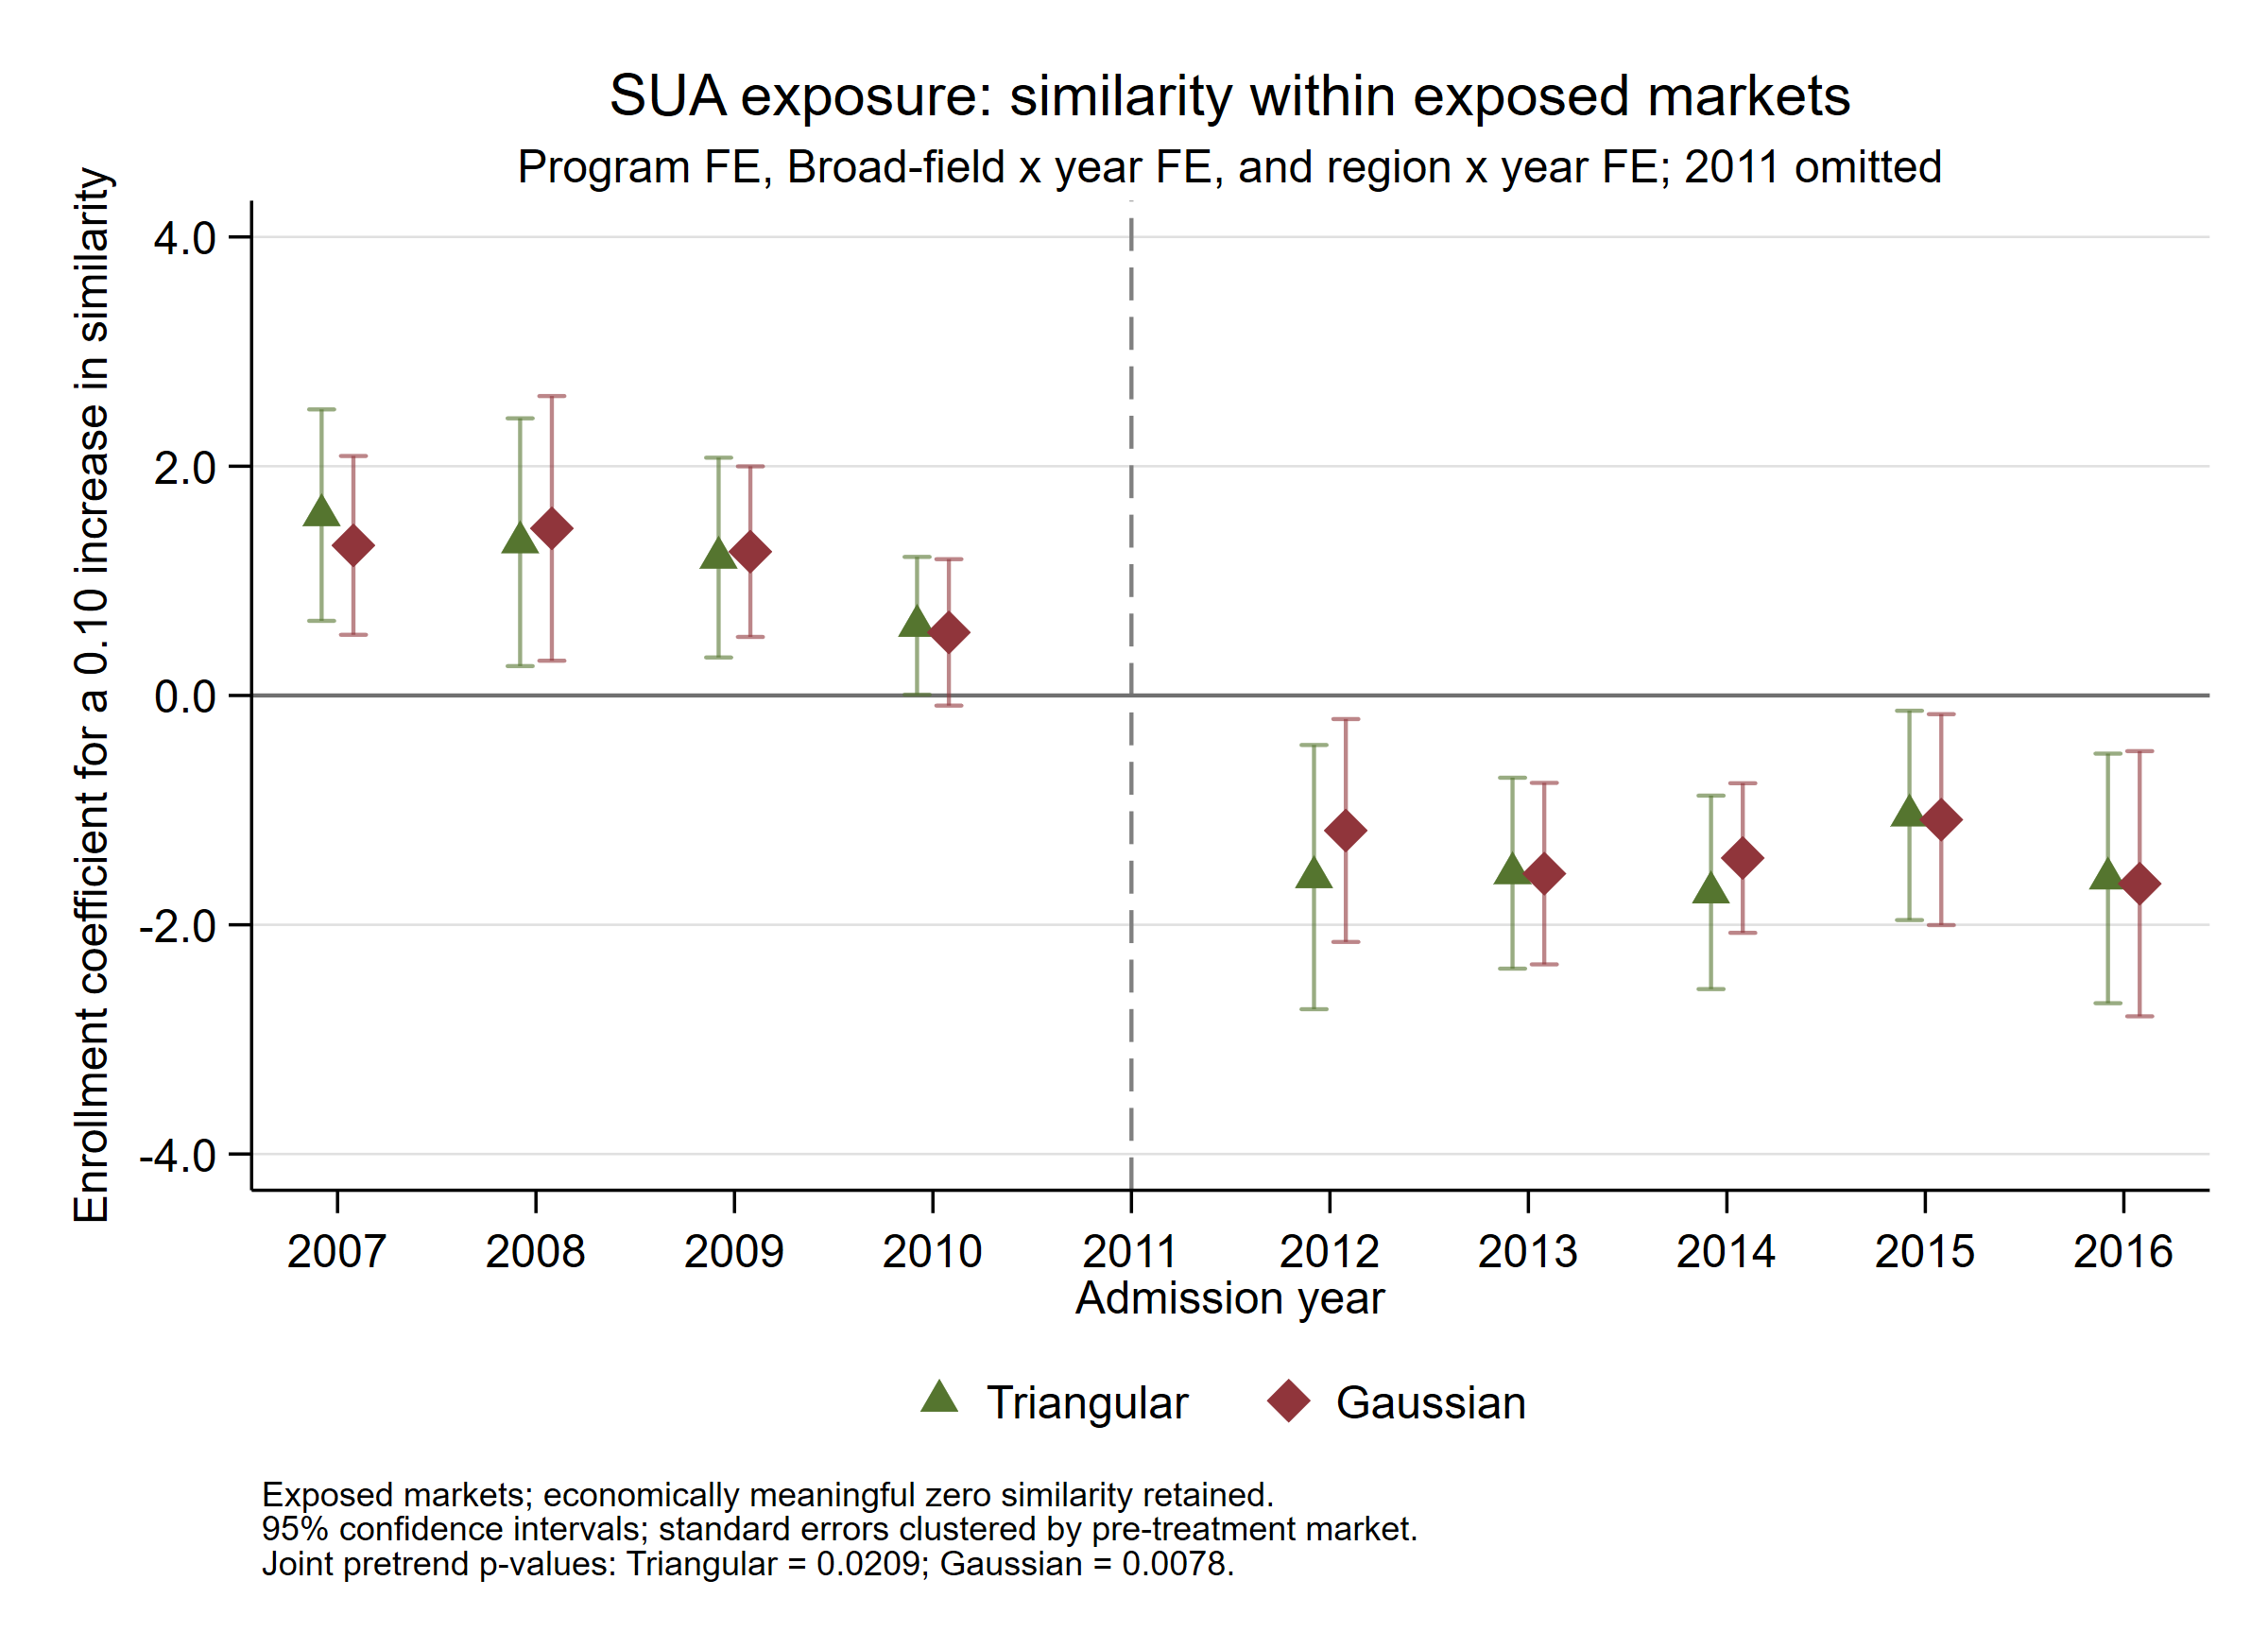
\includegraphics[ width=\linewidth ]{../../output/sua_similarity_event_study_altfe.png}

\end{column}

\begin{column}{0.495\textwidth}
\centering
\textbf{\scriptsize Logs}

\vspace{0.03cm}

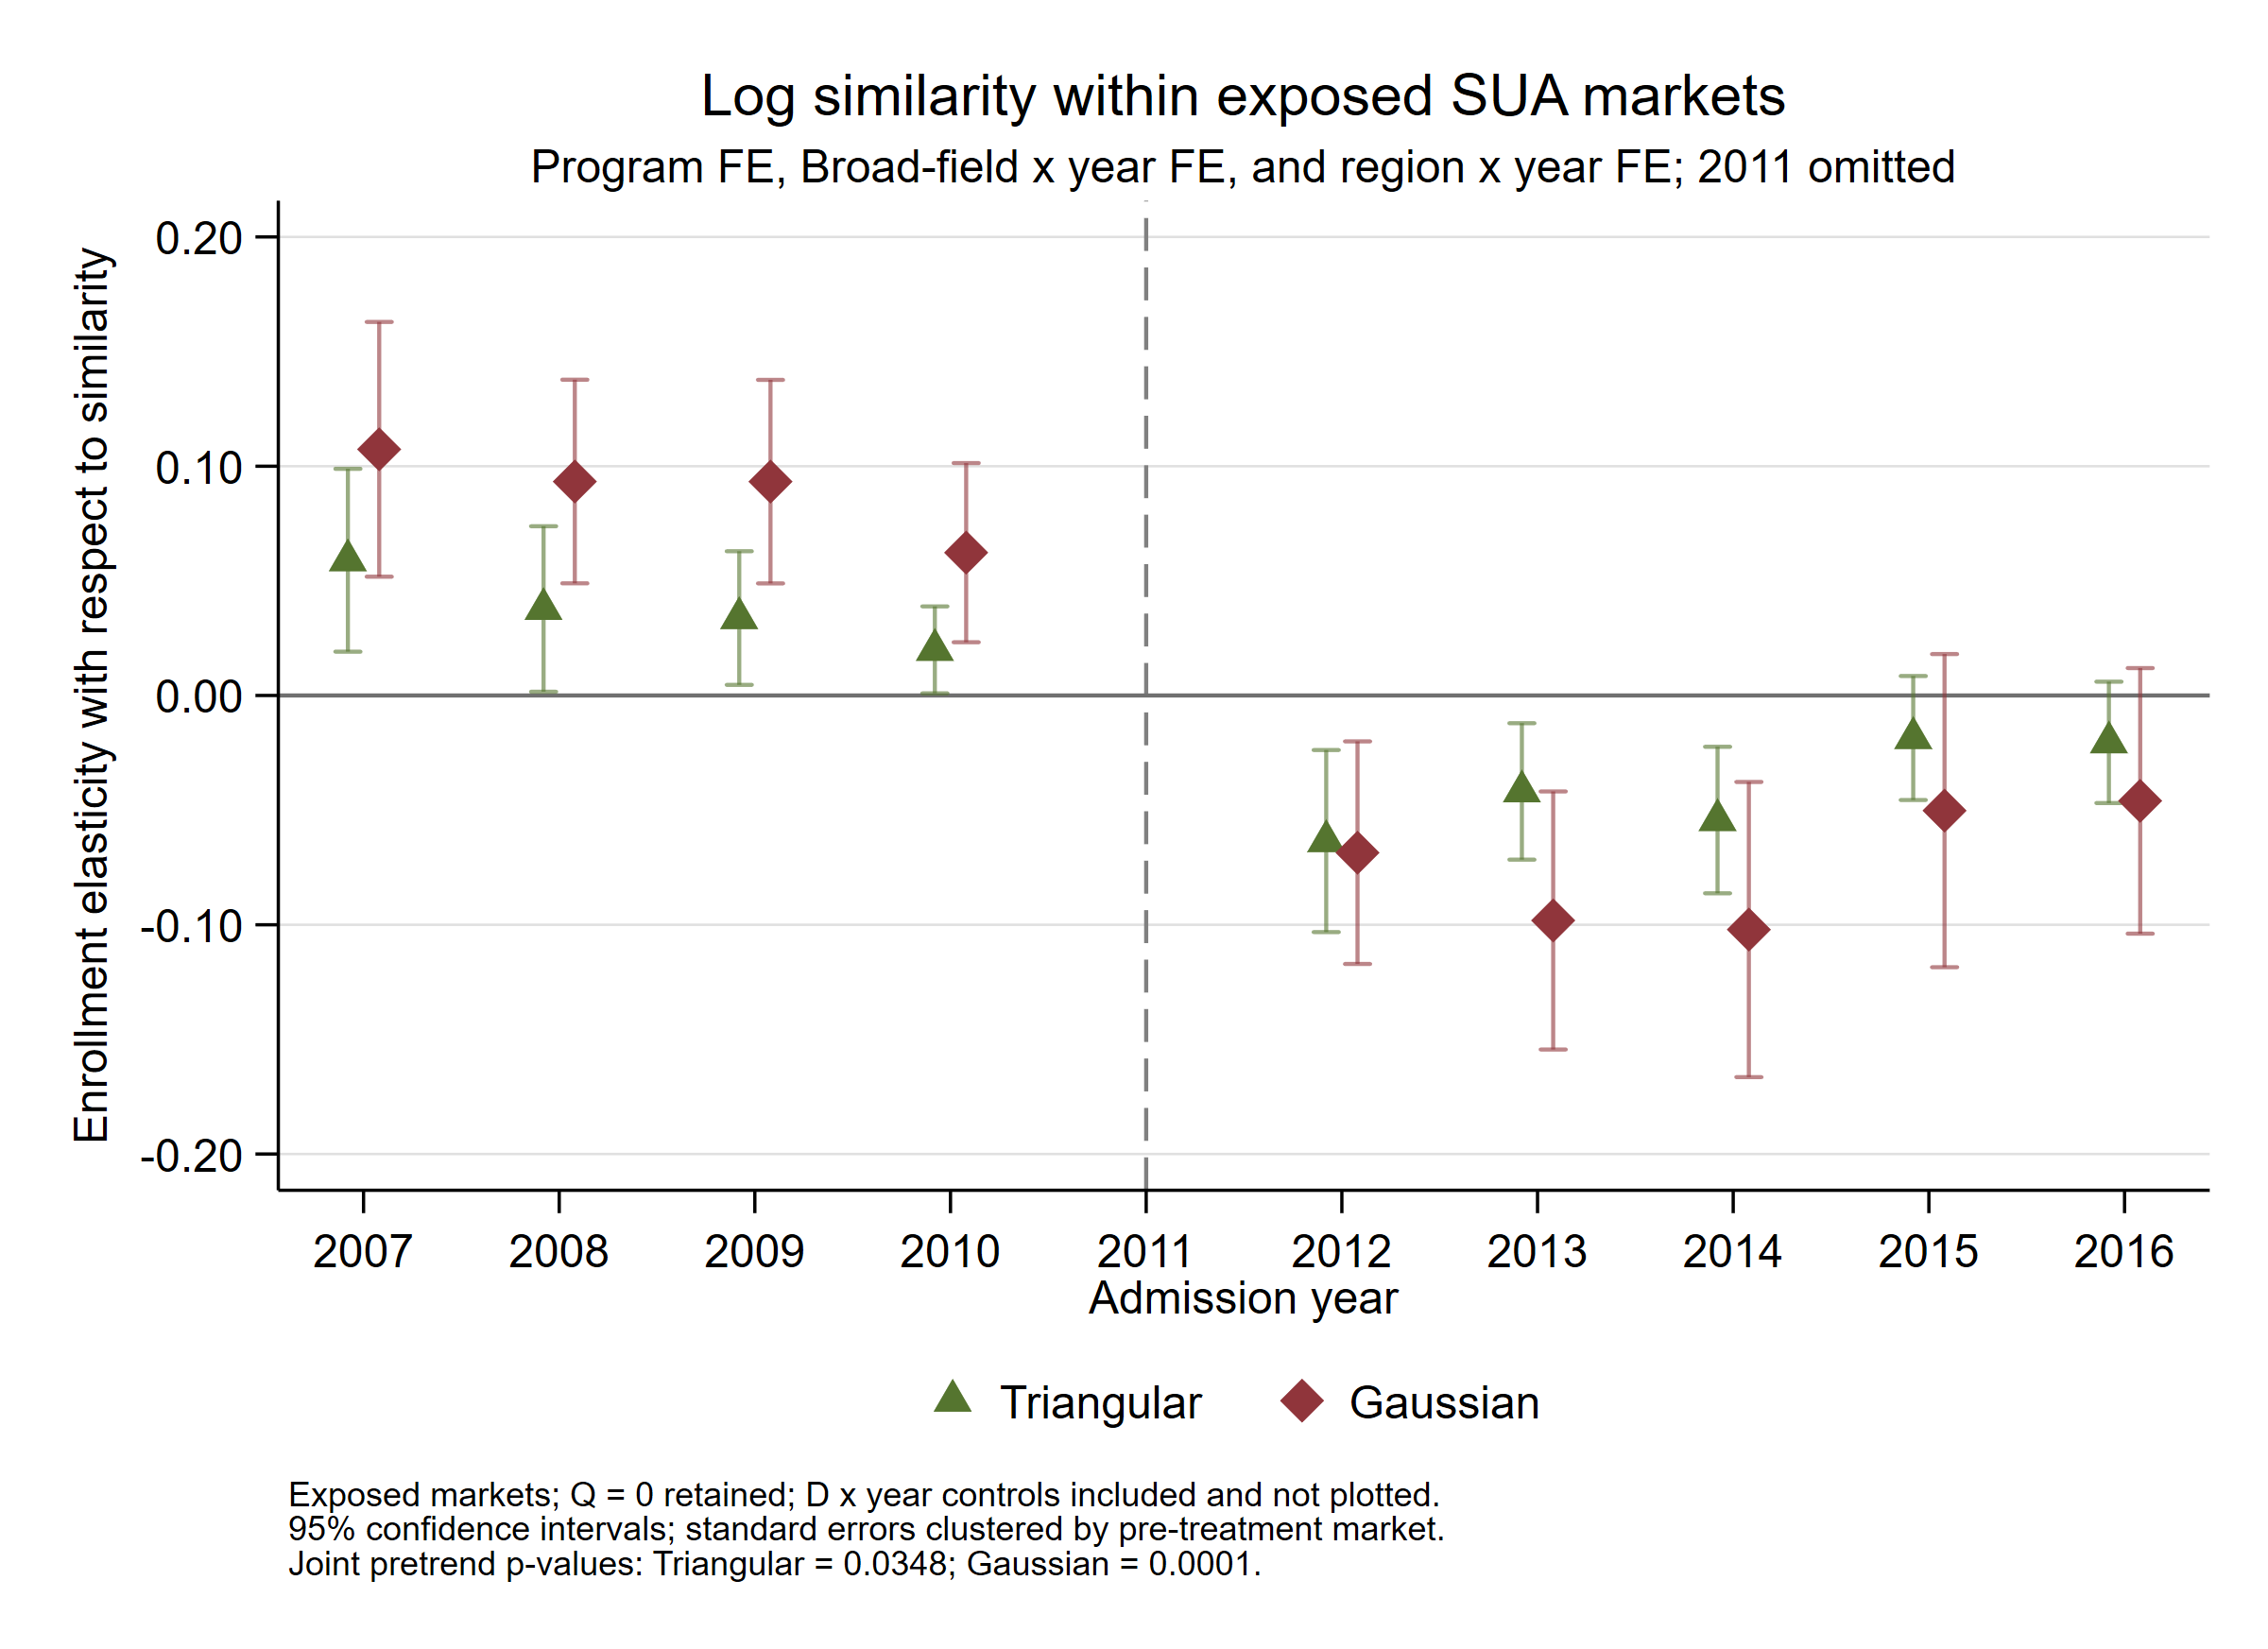
\includegraphics[ width=\linewidth ]{../../output/sua_similarity_log_event_study_altfe.png}

\end{column}

\end{columns}

\vspace{0.06cm}

\parbox{0.96\textwidth}{
\tiny
\textit{Notes:}
Coefficients are relative to 2011.
All models absorb program, Broad-field $\times$ year, and
pre-treatment region $\times$ year fixed effects; standard errors are
clustered by pre-treatment market.
The sample is restricted to markets with positive entrant presence,
$M_m>0$.
Levels retain economically meaningful observations with $Q_p^k=0$.
In logs, zero-similarity observations are also retained by setting
$\widetilde{\log Q_p^k}=0$ when $Q_p^k=0$ and including
$\mathbf{1}\{Q_p^k>0\}\times\mathbf{1}\{t=s\}$ separately in each event year;
these indicator coefficients are not plotted.
Observations with zero first-year enrollment are excluded from the log
specification.
Joint pretrend $p$-values are 0.0209 and 0.0078 for the triangular and
Gaussian measures in levels, and 0.0348 and 0.0001 in logs.
All four tests reject the absence of differential pre-treatment trends at
the 5\% level; estimates are therefore interpreted as descriptive
associations rather than causal effects.
}

\end{frame}

%---------------------------------------------------------


%---------------------------------------------------------
% COSINE EXPOSURE DISTRIBUTIONS: POSITIVE ONLY
%---------------------------------------------------------
\begin{frame}[label=cosine-exposure-positive]

\frametitle{
Cosine exposure distributions conditional on positive exposure
\hfill
\hyperlink{cosine-exposure-main}{
\scriptsize\color{blue}$\leftarrow$ Back
}
}

\centering

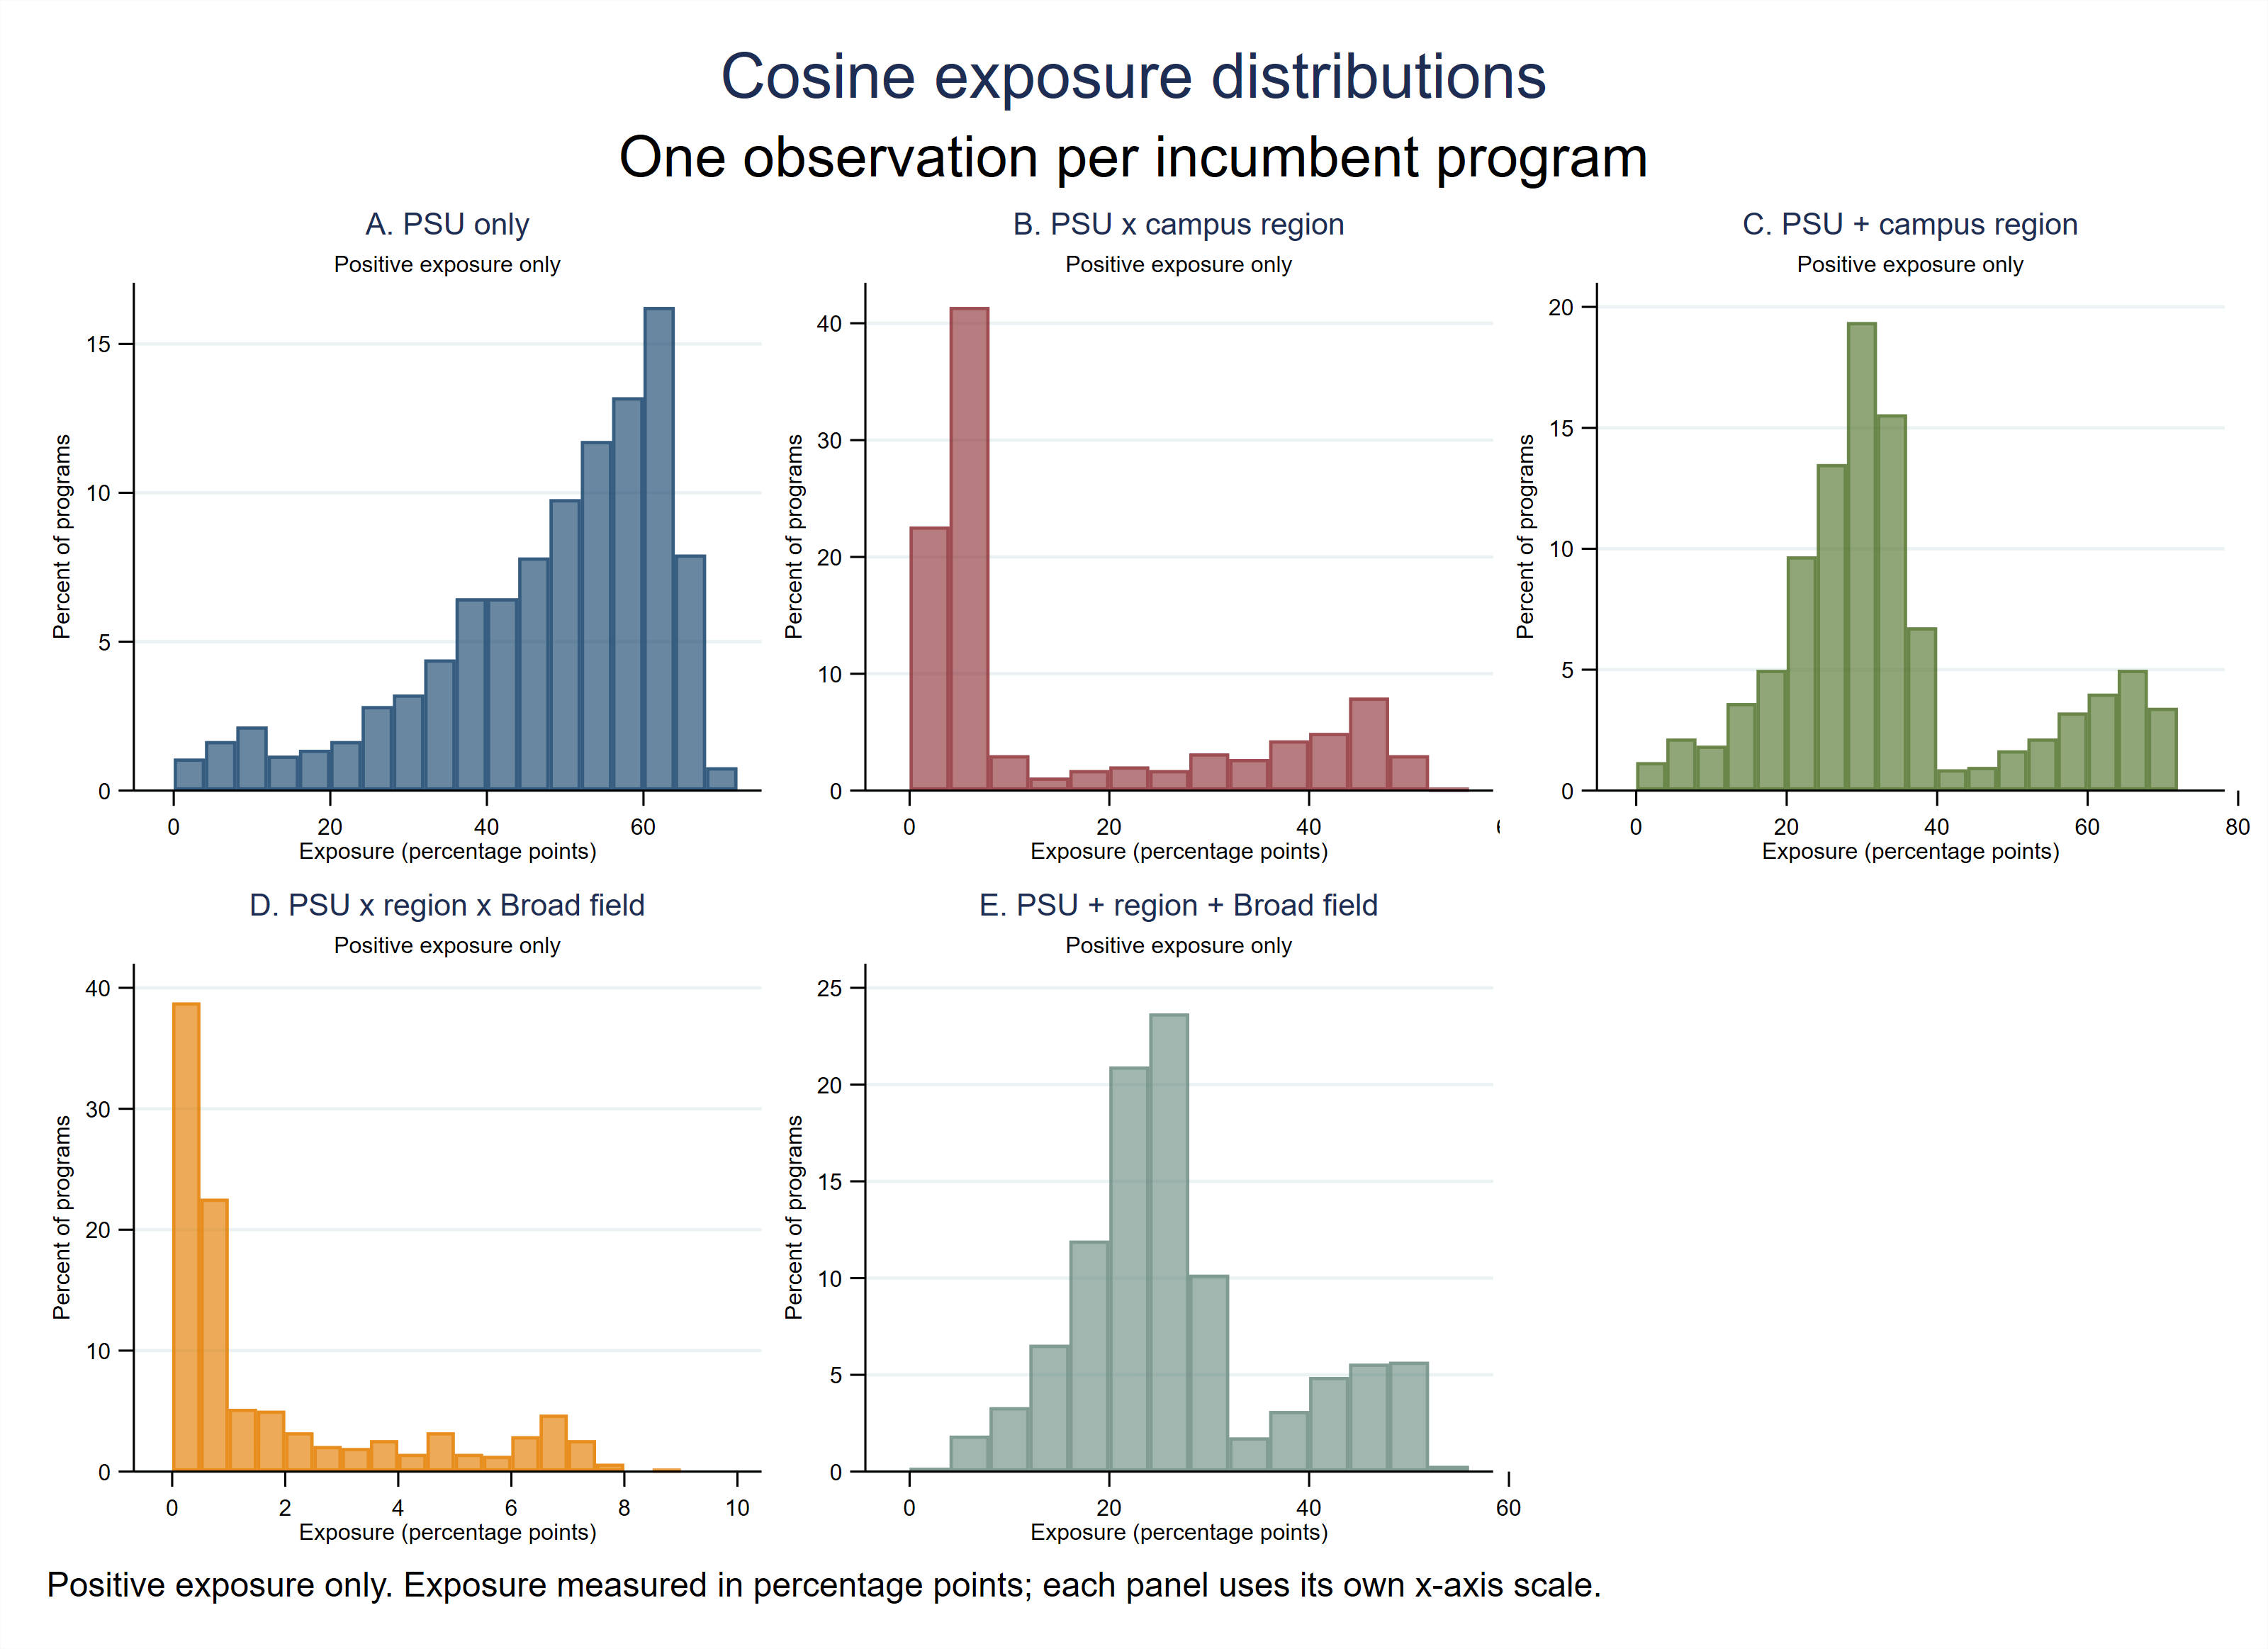
\includegraphics[ width=0.84\textwidth, height=0.68\textheight, keepaspectratio ]{../../output/cosine_exposure_distributions_positive_only.png}

\vspace{-0.10cm}

\begin{itemize}
\scriptsize
\setlength{\itemsep}{2pt}

\item Programs with zero exposure are excluded, allowing the shape of the
positive part of each distribution to be seen more clearly.

\item The multiplicative PSU $\times$ campus region $\times$ Broad field
measure remains concentrated at relatively low exposure values even after
conditioning on positive exposure.

\end{itemize}

\end{frame}

%---------------------------------------------------------
\begin{frame}
\hypertarget{cosine-event-studies}{}
\frametitle{
    Cosine exposure event studies
    \hfill
    \hyperlink{cosine-first-stage}{
        \scriptsize\color{blue}
        $\leftarrow$ First-stage results
    }
}

\begin{figure}
\centering
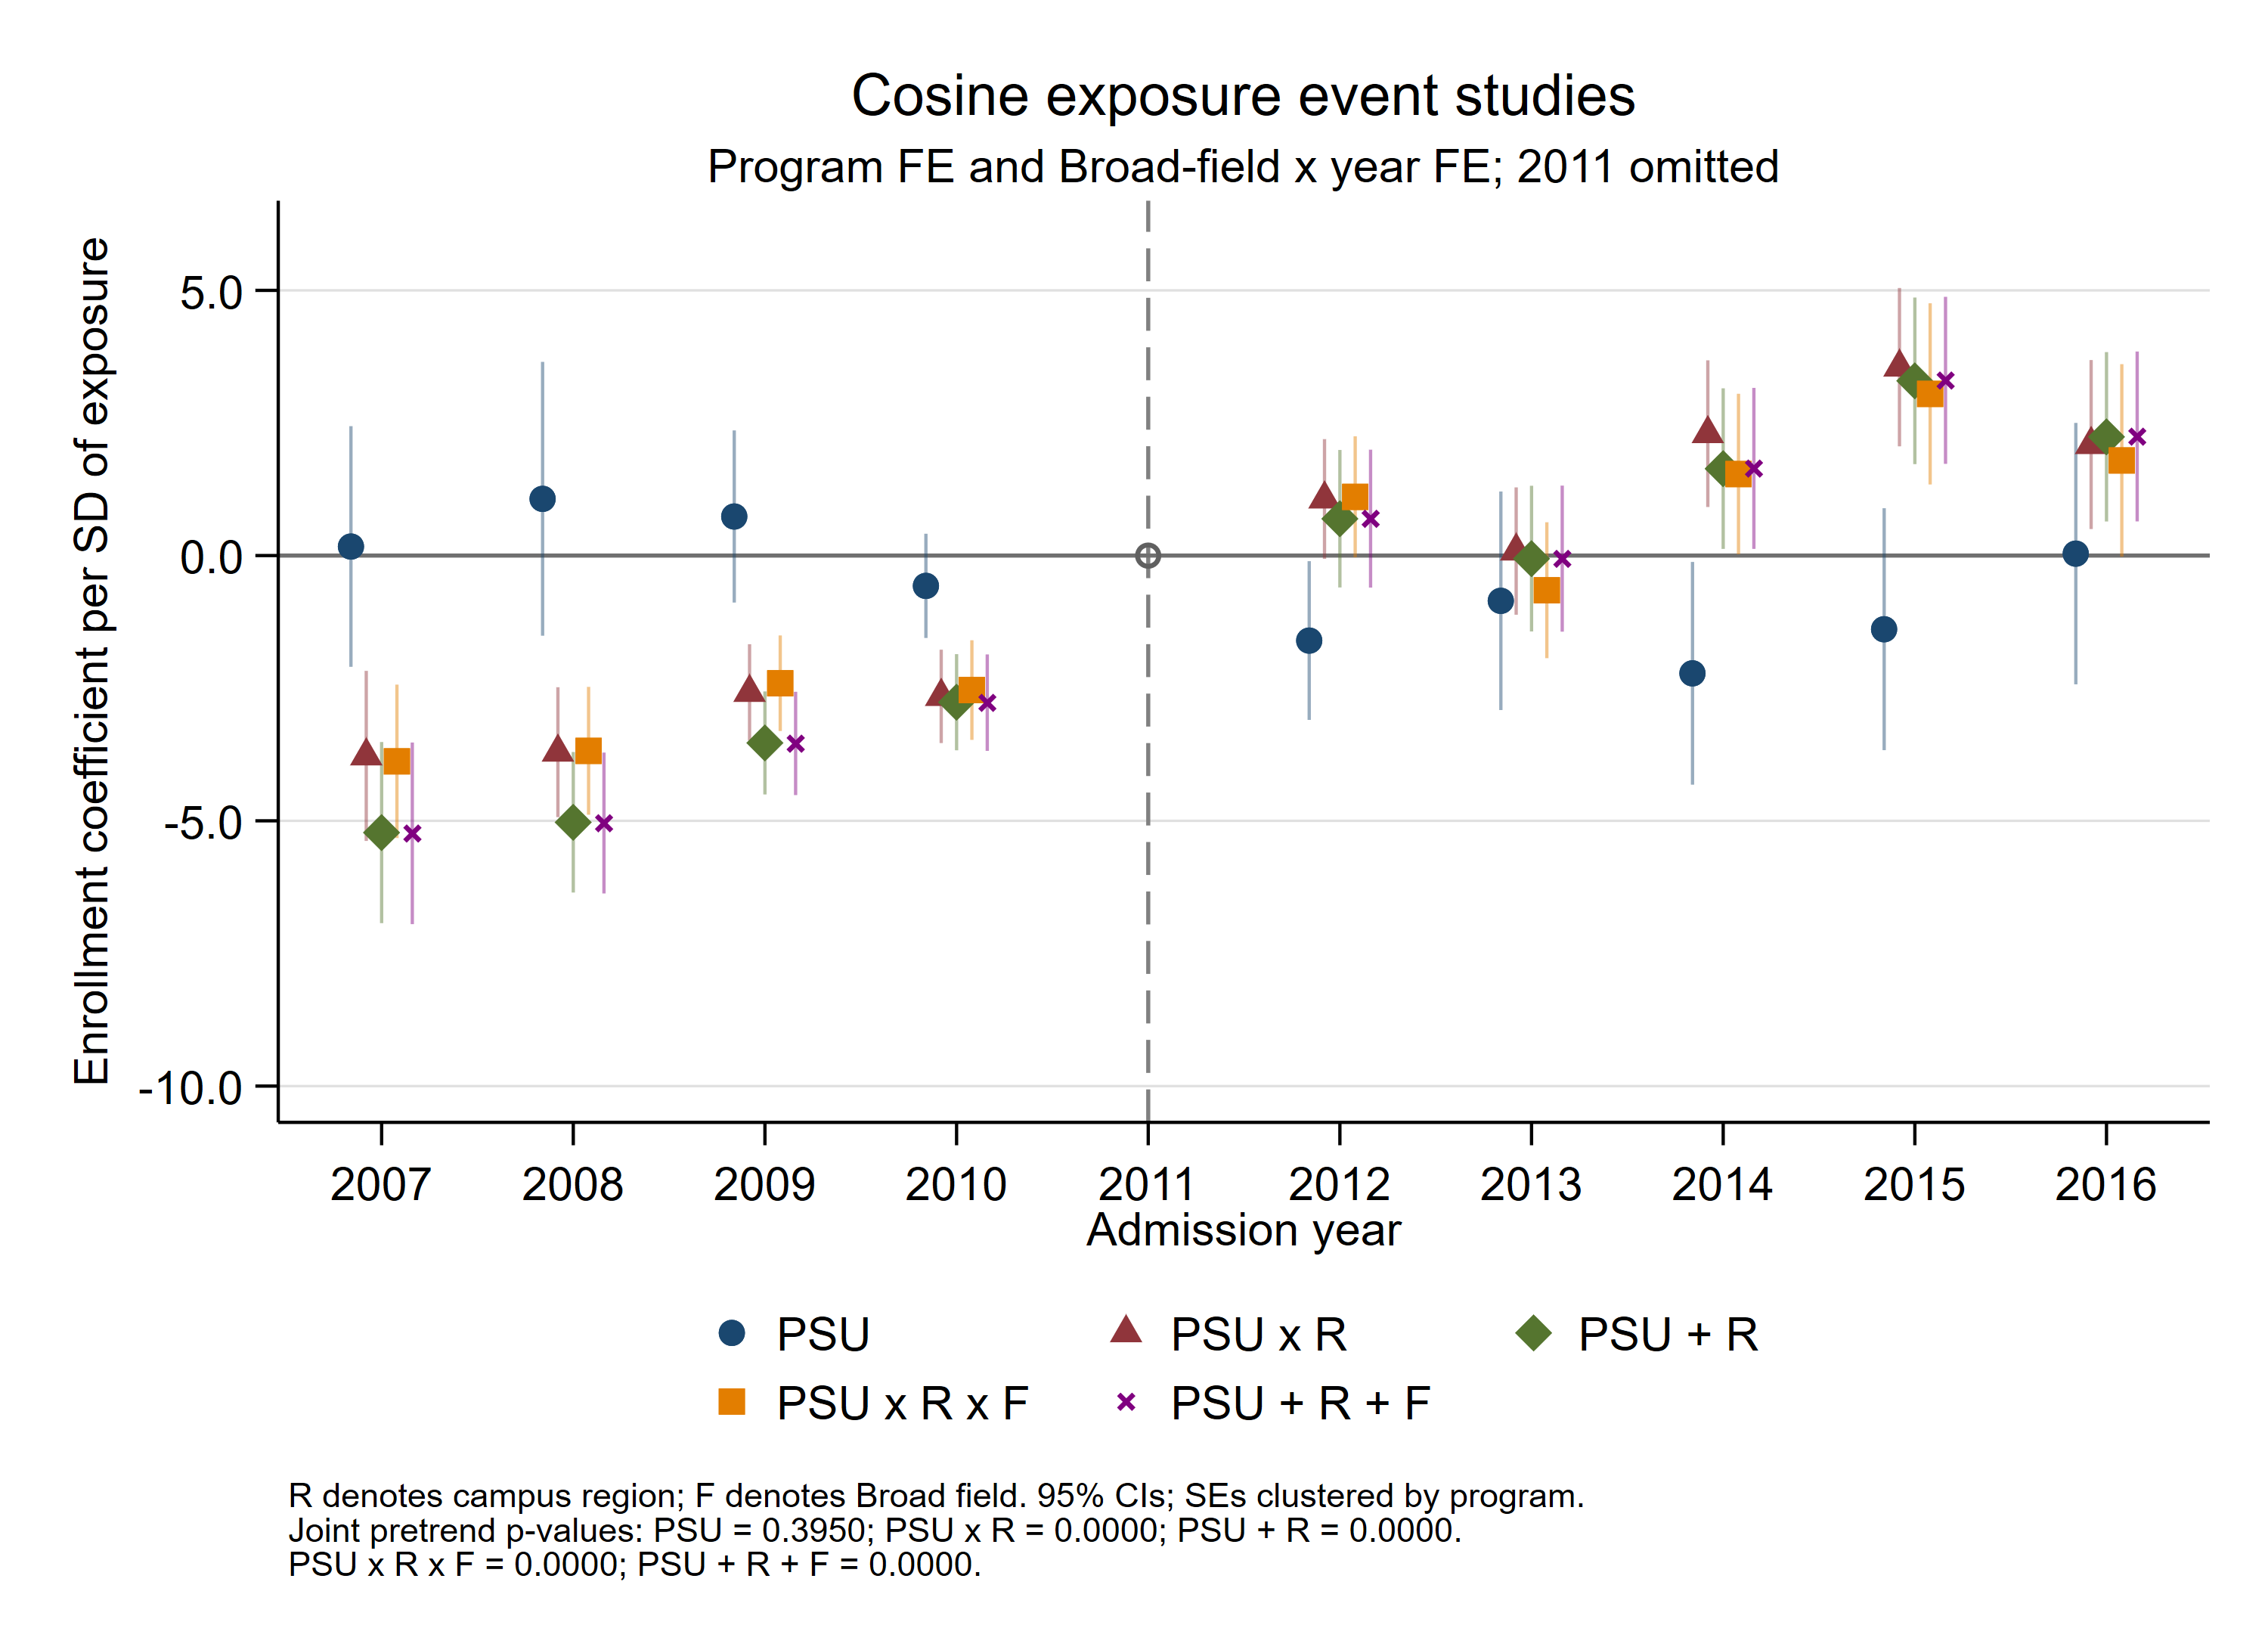
\includegraphics[width=0.49\textwidth]{../../output/cosine_event_studies_baseline.png}
\hfill
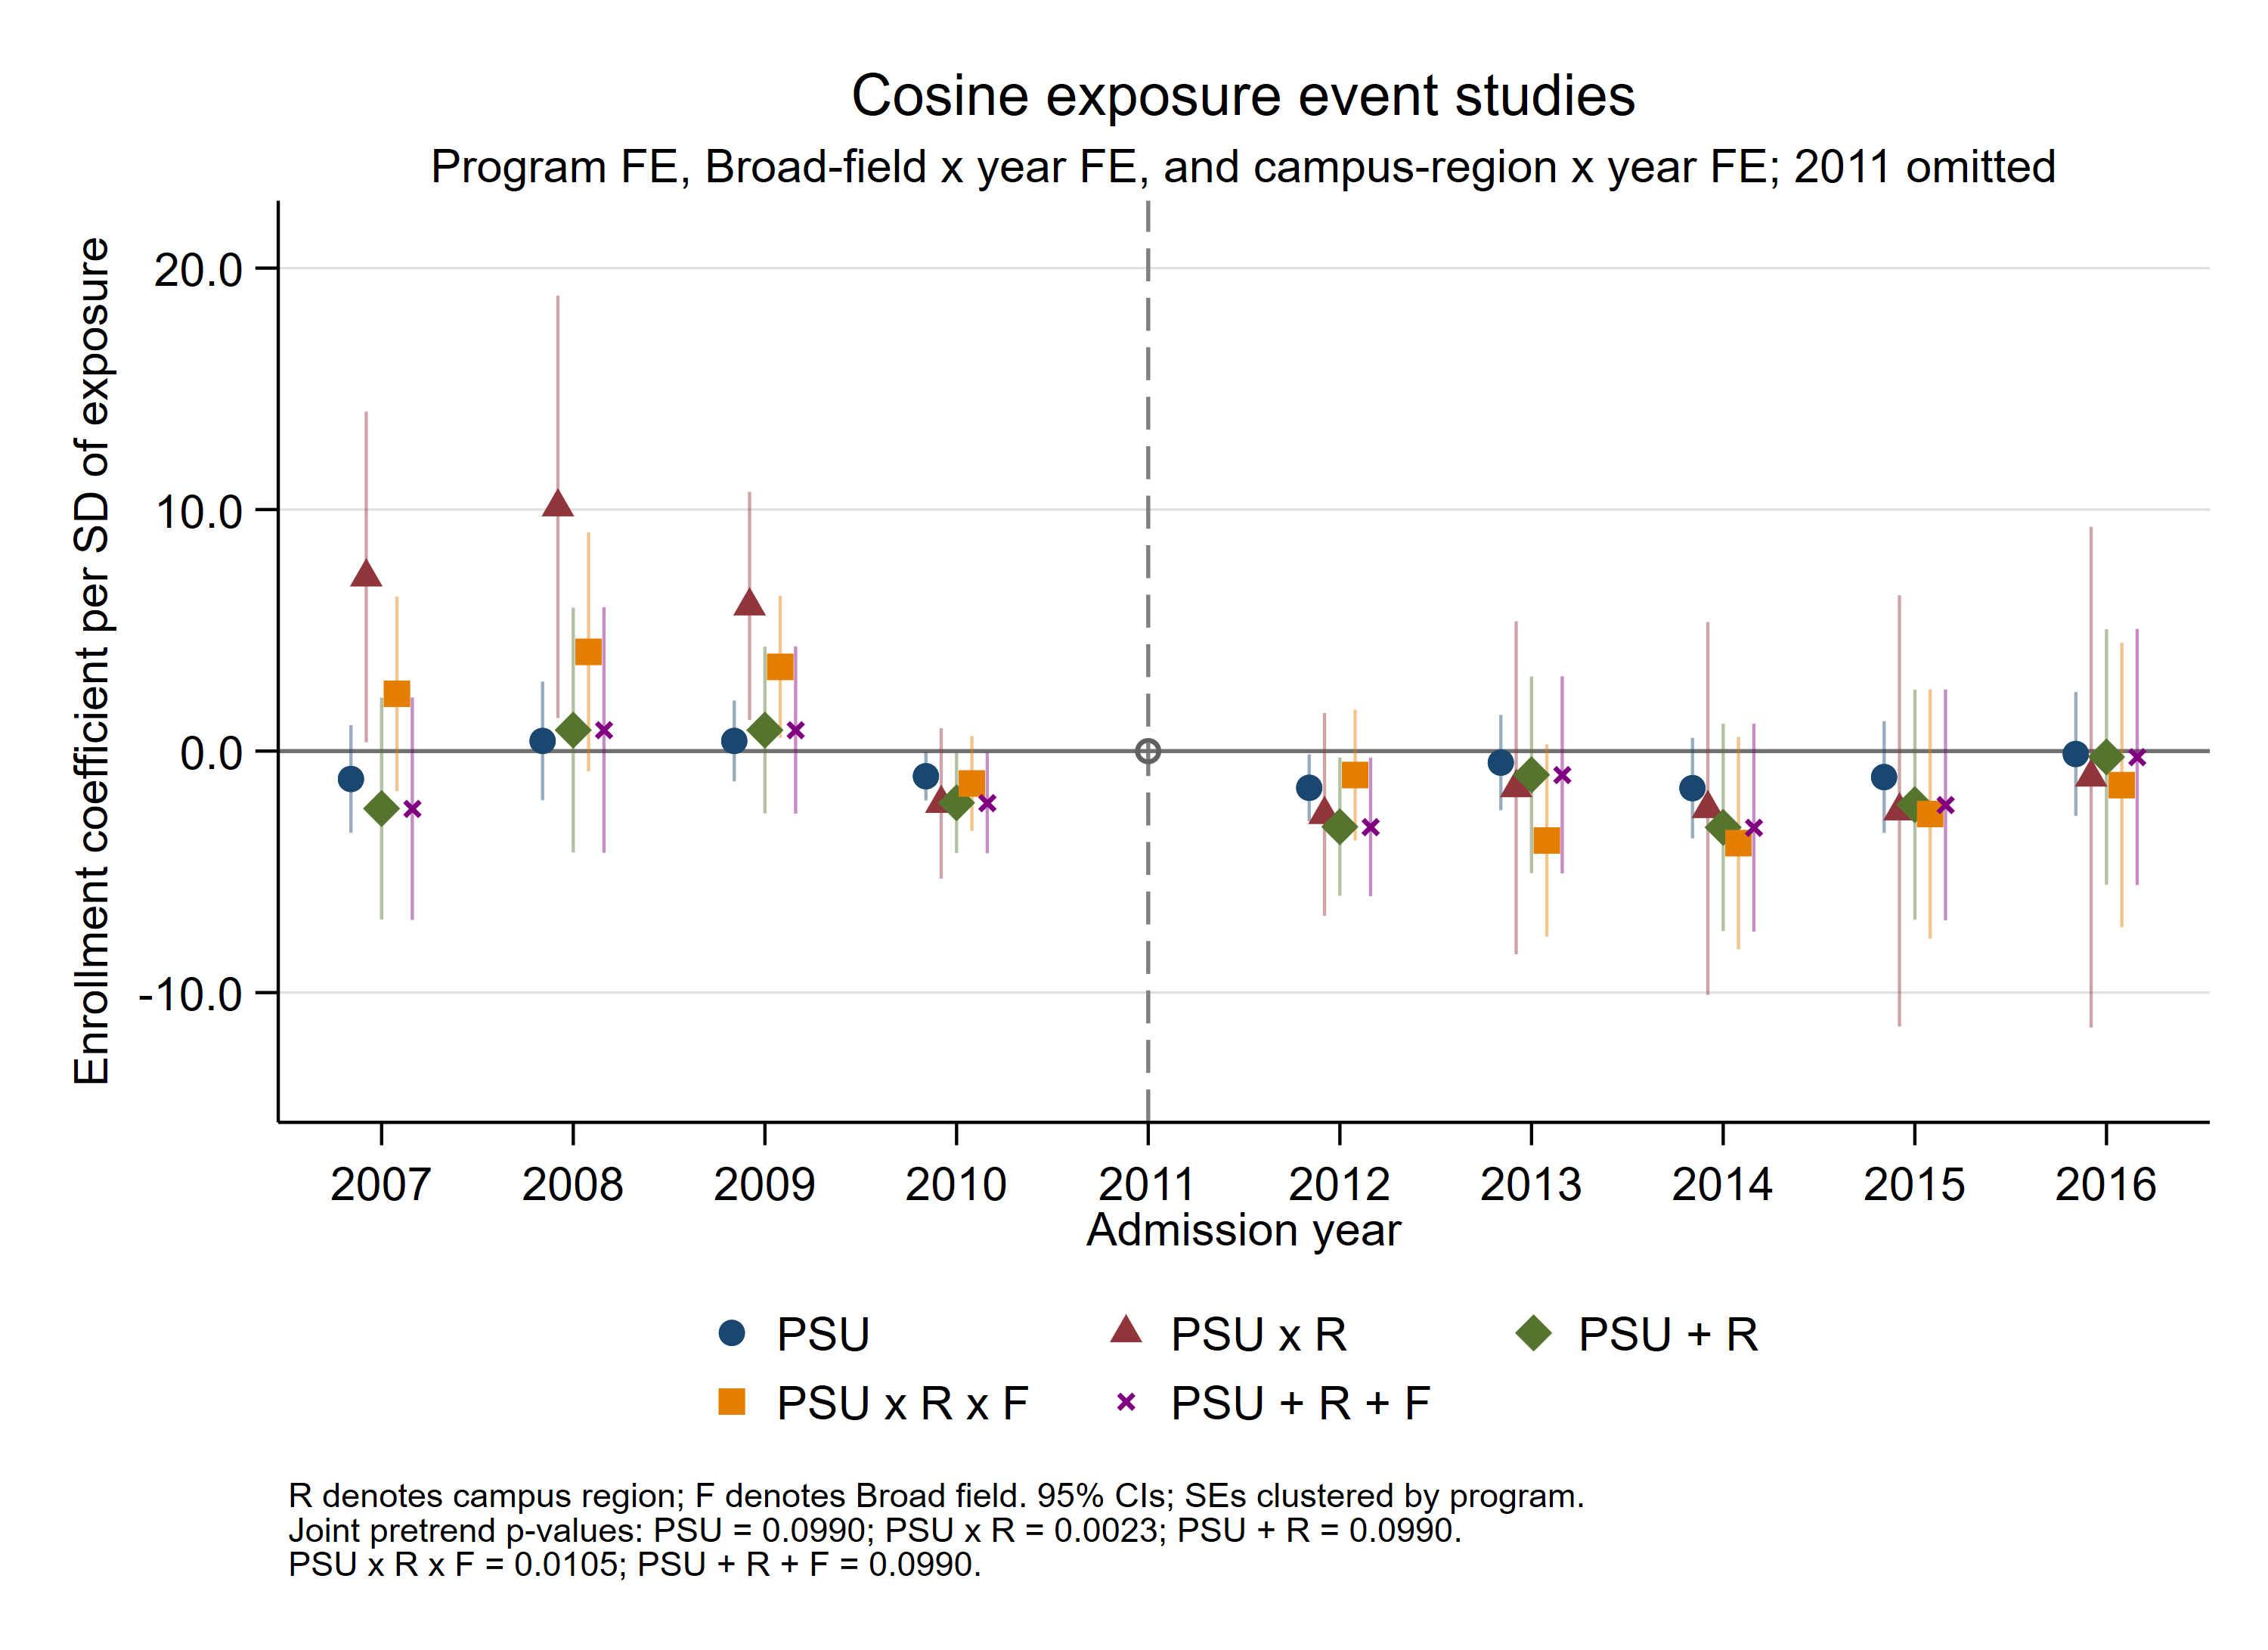
\includegraphics[width=0.49\textwidth]{../../output/cosine_event_studies_regionyear.png}
\end{figure}

\vspace{-0.15cm}

{\tiny
\begin{itemize}

    \item Without campus-region $\times$ year FE, PSU only does not reject joint pretrends ($p=0.395$), but all four measures that incorporate campus region do ($p<0.001$).
    
    \item Adding campus-region $\times$ year FE improves the diagnostic for PSU and the additive measures (all $p=0.099$), but the multiplicative measures still reject: PSU $\times$ region ($p=0.0023$) and PSU $\times$ region $\times$ field ($p=0.0105$).
    
    \item Post-2012 estimates become mostly negative and imprecise once campus-region $\times$ year FE are included. The min-10 sample is not shown and delivers virtually the same conclusions.
    
    \item Overall, the cosine results are best interpreted as descriptive rather than causal.
\end{itemize}
}
\end{frame}


%---------------------------------------------------------
\begin{frame}[label=vs-exposure-appendix]
\frametitle{Design IV exposure: alternative field definitions
\hfill
\hyperlink{vs-exposure-main}{\scriptsize\color{blue}$\leftarrow$ Broad field}}
\begin{columns}[T,onlytextwidth]
\begin{column}{0.495\textwidth}
\centering
\textbf{\scriptsize ISCED-97}

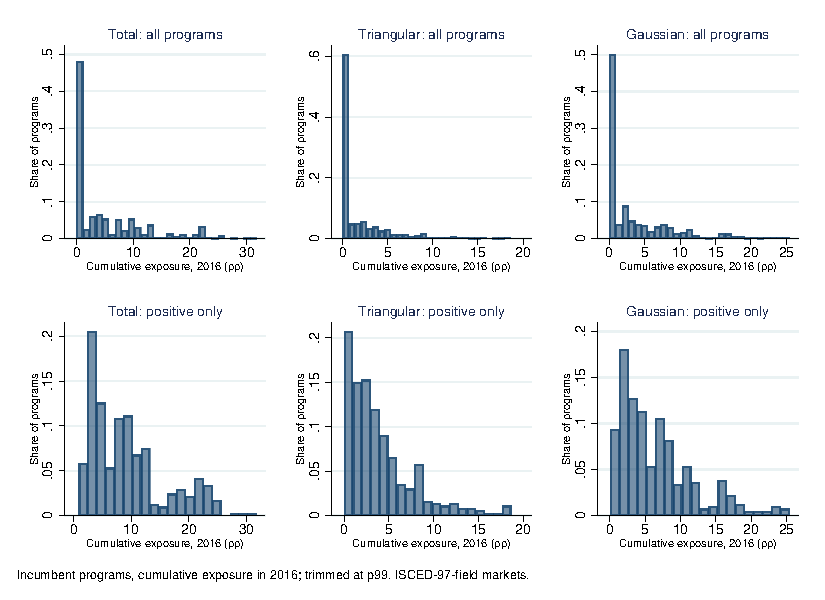
\includegraphics[width=\linewidth, height=0.66\textheight, keepaspectratio]{../../output/vacancy_shocks/figures/vs_exposure_dist_isced.pdf}
\end{column}
\begin{column}{0.495\textwidth}
\centering
\textbf{\scriptsize Generic}

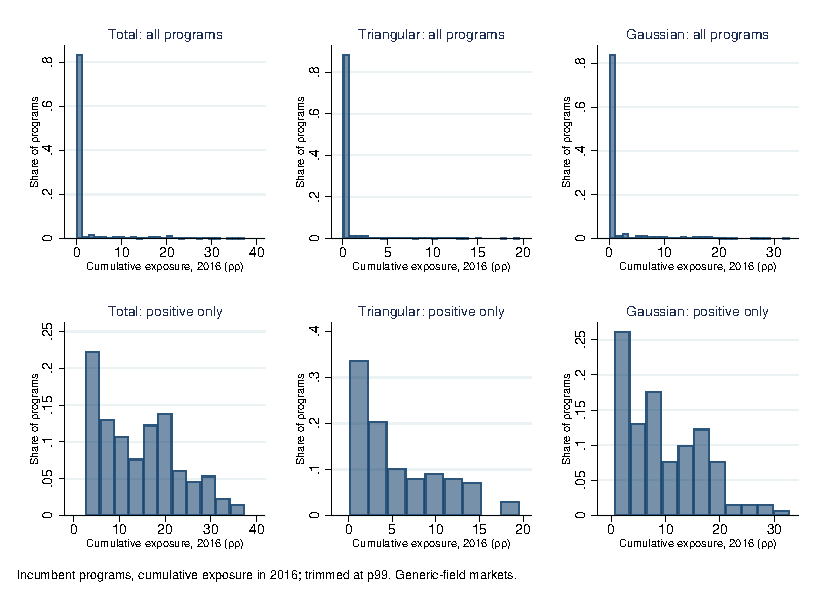
\includegraphics[width=\linewidth, height=0.66\textheight, keepaspectratio]{../../output/vacancy_shocks/figures/vs_exposure_dist_generic.pdf}
\end{column}
\end{columns}
\vspace{0.02cm}
\centering
\tiny
Narrower field definitions generate more markets and more zero-exposure programs: 83\% under the Generic definition.
\end{frame}

%---------------------------------------------------------
\begin{frame}[label=vs-event-studies-mkt]
\frametitle{Design IV event studies: first shock in the market
\hfill
\hyperlink{vs-first-stage}{\scriptsize\color{blue}$\leftarrow$ Levels}\;
\hyperlink{vs-log-first-stage}{\scriptsize\color{blue}$\leftarrow$ Logs}}
\begin{columns}[T,onlytextwidth]
\begin{column}{0.495\textwidth}
\centering
\textbf{\scriptsize First-year enrollment}

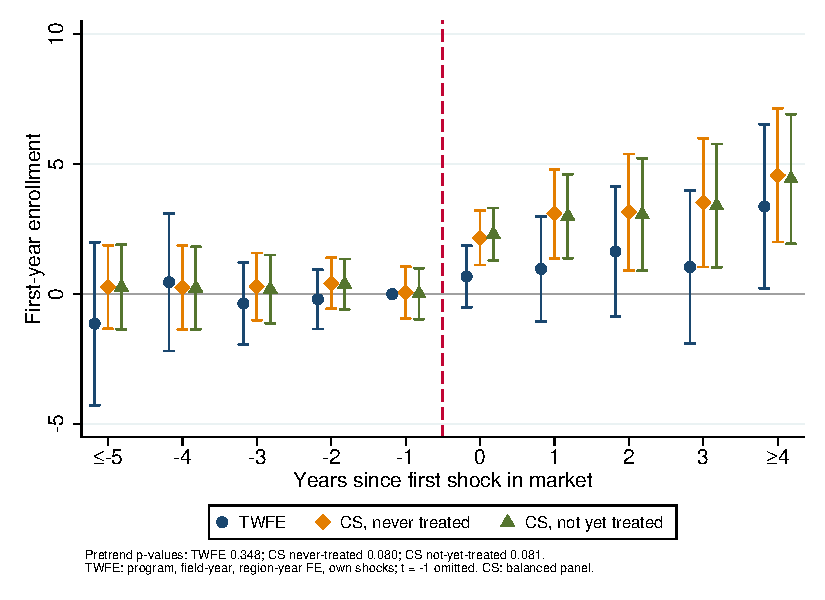
\includegraphics[width=\linewidth]{../../output/vacancy_shocks/figures/vs_es_N_first_mkt.pdf}
\end{column}
\begin{column}{0.495\textwidth}
\centering
\textbf{\scriptsize Log first-year enrollment}

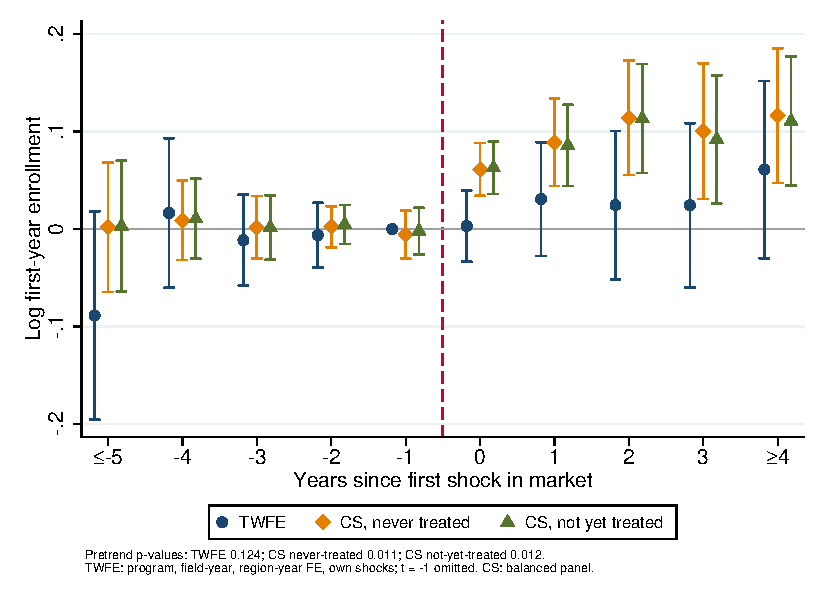
\includegraphics[width=\linewidth]{../../output/vacancy_shocks/figures/vs_es_lnN_mkt.pdf}
\end{column}
\end{columns}
\vspace{0.04cm}
\parbox{0.96\textwidth}{\tiny
\textit{Notes:} $g_k$ is the first year with a shock at another program in $k$'s Broad-field $\times$ region market.
TWFE absorbs program, field $\times$ year and region $\times$ year FE, controls for own shocks, omits $t=-1$ and clusters by
market. Callaway \& Sant'Anna (csdid) uses the balanced panel with never-treated controls (orange) or not-yet-treated plus
never-treated controls (green). 95\% confidence intervals.}
\end{frame}

%---------------------------------------------------------
\begin{frame}[label=vs-event-studies-close]
\frametitle{Design IV event studies: first close-competitor shock
\hfill
\hyperlink{vs-similarity-first-stage}{\scriptsize\color{blue}$\leftarrow$ Back to table}}
\begin{columns}[T,onlytextwidth]
\begin{column}{0.495\textwidth}
\centering
\textbf{\scriptsize First-year enrollment}

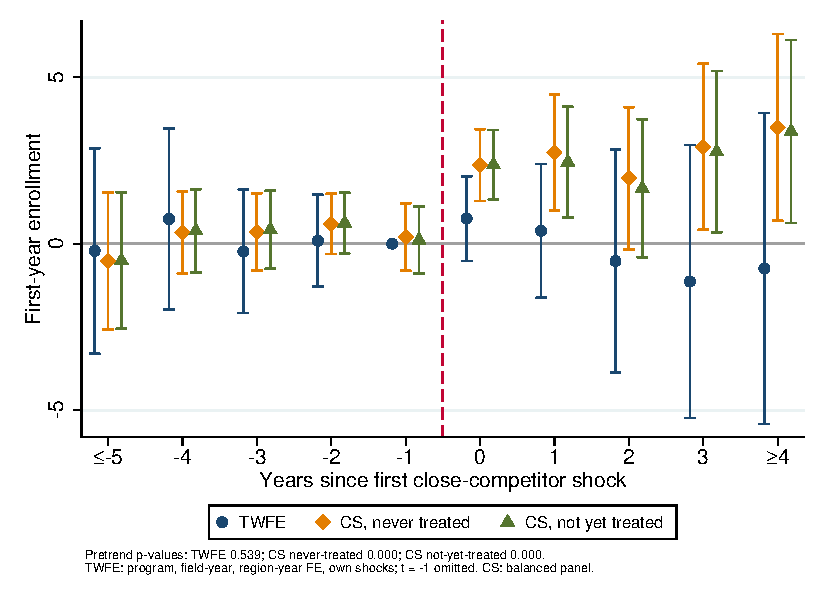
\includegraphics[width=\linewidth]{../../output/vacancy_shocks/figures/vs_es_N_first_close.pdf}
\end{column}
\begin{column}{0.495\textwidth}
\centering
\textbf{\scriptsize Log first-year enrollment}

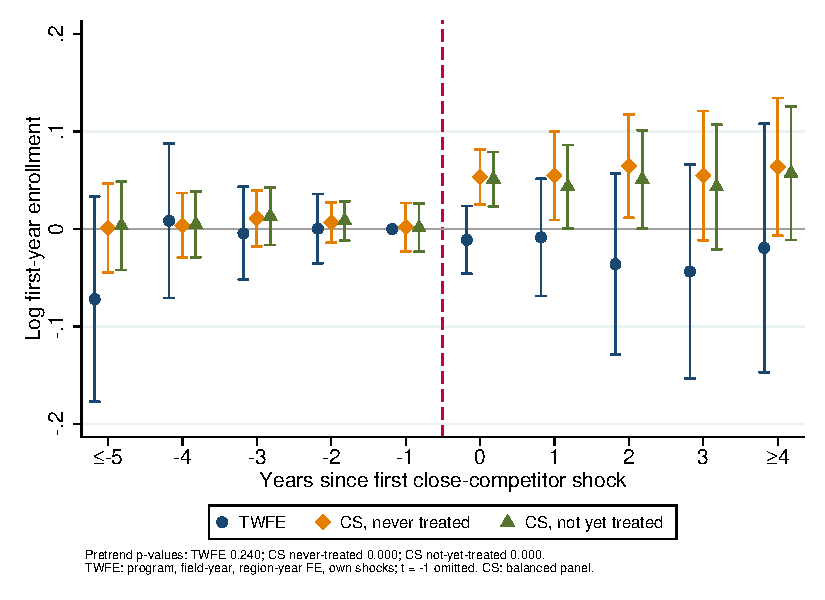
\includegraphics[width=\linewidth]{../../output/vacancy_shocks/figures/vs_es_lnN_close.pdf}
\end{column}
\end{columns}
\vspace{0.04cm}
\parbox{0.96\textwidth}{\tiny
\textit{Notes:} $g_k$ is the first year with a shock at a program in $k$'s Broad-field market whose entrant PSU is within
50 points of $k$'s (the support of the triangular kernel). Estimators as in the previous slide.}
\end{frame}

%---------------------------------------------------------
\begin{frame}[label=vs-cosine-positive]
\frametitle{Design IV cosine exposure, positive exposure only
\hfill
\hyperlink{vs-cosine-main}{\scriptsize\color{blue}$\leftarrow$ Back}}
\centering
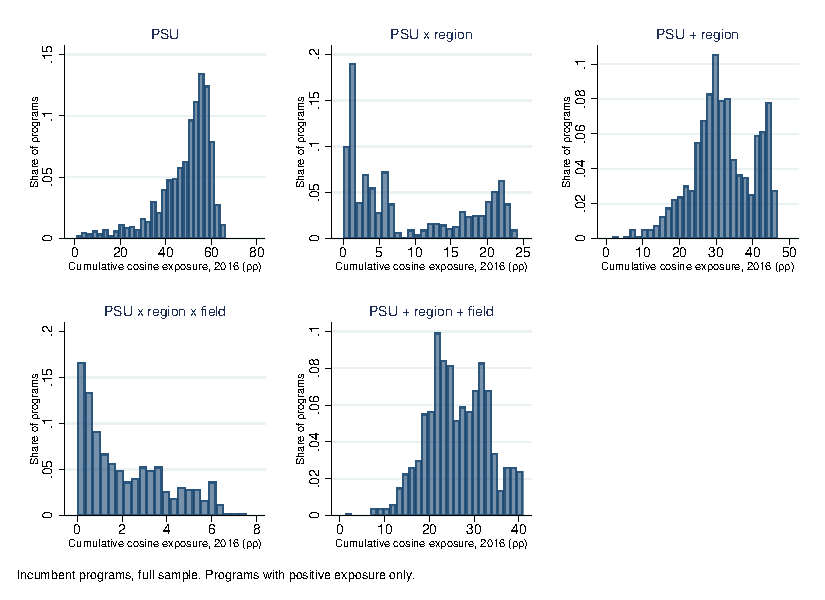
\includegraphics[width=0.82\textwidth, height=0.68\textheight, keepaspectratio]{../../output/vacancy_shocks/figures/vs_cos_dist_pos.pdf}
\end{frame}

%---------------------------------------------------------
\begin{frame}[label=vs-event-studies-cos]
\frametitle{Design IV event studies: top-5 cosine shock
\hfill
\hyperlink{vs-cosine-first-stage}{\scriptsize\color{blue}$\leftarrow$ Cosine results}}
\begin{columns}[T,onlytextwidth]
\begin{column}{0.495\textwidth}
\centering
\textbf{\scriptsize First-year enrollment}

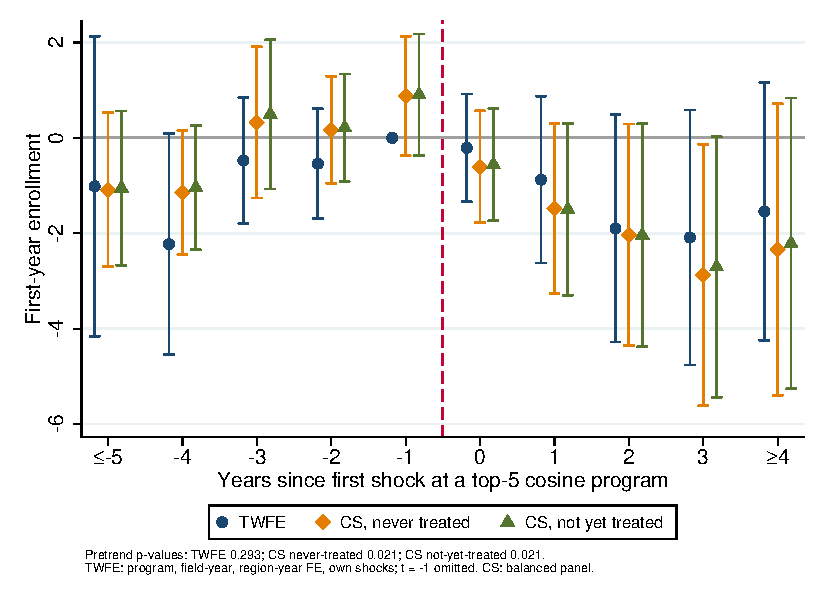
\includegraphics[width=\linewidth]{../../output/vacancy_shocks/figures/vs_es_N_first_cos.pdf}
\end{column}
\begin{column}{0.495\textwidth}
\centering
\textbf{\scriptsize Log first-year enrollment}

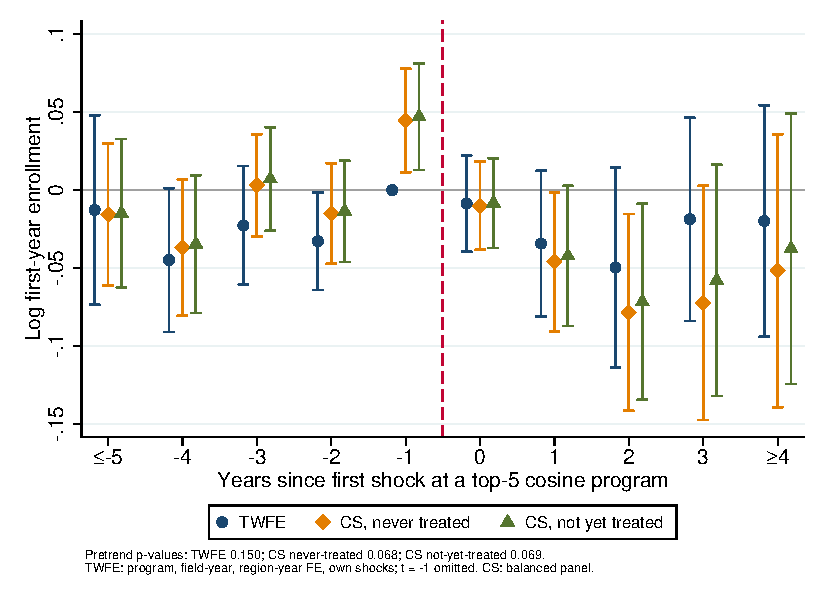
\includegraphics[width=\linewidth]{../../output/vacancy_shocks/figures/vs_es_lnN_cos.pdf}
\end{column}
\end{columns}
\vspace{0.04cm}
\parbox{0.96\textwidth}{\tiny
\textit{Notes:} $g_k$ is the first year with a shock at one of the five programs with the highest PSU-bin cosine
similarity to $k$, anywhere in the country. TWFE clusters by program. Estimators as in the market-shock slide.}
\end{frame}


\end{document}
